\documentclass[pdflatex,sn-nature]{sn-jnl}

% Standard packages for Nature journals
\geometry{margin=0.75in}
\usepackage{graphicx}
\usepackage{amsmath,amssymb,amsfonts}
\usepackage{booktabs}
\usepackage{multirow}
\usepackage{textcomp}
\usepackage{longtable}
\usepackage{array}
\usepackage{calc}
\usepackage{tabularx}
\usepackage{fp}  % For \real command in table calculations
\usepackage{caption}
\usepackage[nameinlink,capitalize]{cleveref}
\usepackage{float}
\usepackage{placeins}
\usepackage{tikz}
\usetikzlibrary{arrows.meta,calc,positioning,shapes.geometric}


% Define pandocbounded macro for pandoc compatibility
\makeatletter
\def\pandocbounded#1{%
  \begingroup
  % Override any existing includegraphics settings to ensure proper sizing
  \setkeys{Gin}{width=1.0\linewidth,height=1.0\textheight,keepaspectratio}%
  #1%
  \endgroup
}
\makeatother

% Define \real command for table calculations (used by pandoc)
\makeatletter
\def\real#1{#1}
\makeatother

% Define pandoc-generated list commands
\providecommand{\tightlist}{%
  \setlength{\itemsep}{0pt}\setlength{\parskip}{0pt}}

% Define other common pandoc commands that might be missing
\providecommand{\passthrough}[1]{#1}
\providecommand{\BeginKnitrBlock}[1]{}
\providecommand{\EndKnitrBlock}[1]{}

% Handle pandoc's CSL citations if they appear
\newcommand{\cslhangindent}[1]{}
\newcommand{\cslentryspacingunit}[1]{}
\newcommand{\cslreferences}[2]{}

\captionsetup[figure]{name=Supplementary Figure}
\renewcommand{\thefigure}{S\arabic{figure}}
\renewcommand{\thetable}{S\arabic{table}}
\captionsetup[table]{name=Supplementary Table}

% Customize List of Figures and List of Tables to include "Supplementary"
\renewcommand{\listfigurename}{List of Supplementary Figures}
\renewcommand{\listtablename}{List of Supplementary Tables}

% Add "Supplementary Figure/Table" prefix to entries with proper hyperlinks
\makeatletter
\let\oldnumberline\numberline
\def\numberline#1{\oldnumberline{#1}}

\let\oldcontentsline\contentsline
\def\contentsline#1#2#3#4{%
  \def\tempa{figure}%
  \def\tempb{table}%
  \def\tempc{#1}%
  \ifx\tempc\tempa
    \oldcontentsline{#1}{Supplementary Figure #2}{#3}{#4}%
  \else
    \ifx\tempc\tempb
      \oldcontentsline{#1}{Supplementary Table #2}{#3}{#4}%
    \else
      \oldcontentsline{#1}{#2}{#3}{#4}%
    \fi
  \fi
}
\makeatother


\begin{document}
\title{Somatic haplotype reconstruction and variant recalibration from tumor-only long-read sequencing (Supplementary Information)}

\author{\fnm{Zhen-Yu} \sur{Chen}\textsuperscript{1}}
\author{\fnm{Zhenxian} \sur{Zheng}\textsuperscript{2}}
\author{\fnm{Ruibang} \sur{Luo}\textsuperscript{2}}
\author{\fnm{Hsu-Fen} \sur{Fu}\textsuperscript{1}}
\author{\fnm{Yung-Jen} \sur{Yang}\textsuperscript{1}}
\author*{\fnm{Yao-Ting} \sur{Huang}\textsuperscript{1}*}\email{ythuang@cs.ccu.edu.tw}

\affil[1]{\orgdiv{Department of Computer Science and Information Engineering}, \orgname{National Chung Cheng University}, \country{Taiwan}}
\affil[2]{\orgdiv{School of Computing and Data Science}, \orgname{The University of Hong Kong}, \city{Hong Kong}, \country{China}}

\maketitle

% Table of Contents
\tableofcontents

% List of Figures
\listoffigures

% List of Tables
\listoftables
\clearpage

\section{Supplementary Results}

\subsection{Robustness of somatic recalibration to the ClairS-TO model}\label{characterization-of-the-precision-recall-trade-off-using-simulation-trained-models}

To test whether the recalibration depends on the particular ClairS-TO model, we repeated the SNV benchmark with a ClairS-TO model trained on simulated data (ClairS-TO-ss), with and without LongPhase-TO, across the same eight datasets and DNA fraction levels (Supplementary Figure~\ref{fig:met-page-32-cropped-jpg}).

The fraction-dependent profile observed for the default model was reproduced. Recalibration raised precision across 20 to 80\% DNA fraction in nearly every dataset, at a modest cost to recall, and the F1 gain was largest at low DNA fraction and in the two datasets where the standalone precision of ClairS-TO-ss was lowest (HCC1937\_UCSC and HCC1954\_UCSC). At 100\% DNA fraction, where ClairS-TO-ss was already most precise, recalibration lowered F1 in several datasets. The recalibration therefore acts as a conservative precision filter whose benefit concentrates where the standalone caller is least reliable, regardless of the ClairS-TO model used.

\subsection{Cross-platform generalization of somatic recalibration to PacBio HiFi}\label{supp:pacbio-recalibration}

Every model used by the triplet-graph recalibration was fitted once on nanopore data and then held fixed: the linear (indel) and third-order polynomial (SNV) predictors were trained on the HCC1395\_HKU mixture at 0.6 tumor DNA fraction, and the site-level decision thresholds ($S_H>0.8$ and $L/(L+N)\ge0.2$) were calibrated on the same sample. To test whether this haplotype-based recalibration depends on the sequencing platform, we applied the identical models and thresholds to six PacBio HiFi datasets (Supplementary Table~\ref{tab:pacbio-datasets}), using the same \emph{in silico} dilution design spanning 20--100\% tumor DNA fraction. Five of these cell lines (HCC1395, HCC1937, HCC1954, H1437 and H2009) belong to the PacBio Revio tumor-normal cohort assembled for DeepSomatic, four of them obtained here from the CASTLE release and HCC1395 from the public PacBio Revio 2023Q2 release. COLO829 is an independent PacBio Revio benchmark from the same public release. The panel is therefore not the complete DeepSomatic cohort, which also includes Hs578T.

Every LongPhase-TO model was held off-platform. Both somatic callers were run with their PacBio HiFi models, so that the baselines against which recalibration is measured are platform-matched, whereas LongPhase-TO was run in its nanopore mode so that the nanopore-fitted triplet-graph coefficients were applied under exactly the settings in which they were trained. No coefficient was refitted and no threshold was retuned for PacBio. The estimation of tumor DNA fraction and ploidy has no trained coefficients and is assessed in the following subsection. The experiment therefore measures transfer of the trained models alone, against callers that carry no comparable platform handicap.

Recalibration improved PacBio HiFi somatic calls to a degree comparable with nanopore. DeepSomatic-TO values are from the configuration with the ClairS-TO normal panels. Averaged over the six datasets and five DNA-fraction levels, mean SNV F1 rose from 0.58 to 0.67 for ClairS-TO and from 0.60 to 0.72 for DeepSomatic-TO, improving 28 and 26 of 30 individual points, respectively (Supplementary Figure~\ref{fig:pacbio-snv-recalibration}). Mean indel F1 rose from 0.24 to 0.27 for ClairS-TO and from 0.28 to 0.37 for DeepSomatic-TO, improving 27 and 28 of 30 points (Supplementary Figure~\ref{fig:pacbio-indel-recalibration}). The gain was precision-driven, as on nanopore. For SNVs, mean precision rose by 0.18 for ClairS-TO at unchanged recall and by 0.23 for DeepSomatic-TO at a recall cost of 0.10. Indels followed the same pattern, with precision gains of 0.11 and 0.35 and recall costs of 0.01 and 0.06. DeepSomatic-TO recall decreased at all 30 points in both variant classes, whereas its precision increased at all 30. Per-mixture precision, recall and F1 for every caller and configuration are given in Supplementary Tables~\ref{tab:pacbio_somatic_snv} and~\ref{tab:pacbio_somatic_indel}.

The dependence on tumor DNA fraction also reproduced the nanopore pattern. Mean SNV F1 gains were largest at low-to-intermediate fraction, reaching $+0.12$, $+0.13$ and $+0.13$ for ClairS-TO and $+0.13$, $+0.15$ and $+0.16$ for DeepSomatic-TO at fractions of 0.2, 0.4 and 0.6, and were smallest at 1.0 ($+0.01$ and $+0.03$). Restricted to mixtures below 1.0, mean SNV F1 increased by 0.12 for ClairS-TO and 0.14 for DeepSomatic-TO, with 23 and 21 of 24 points improved. HCC1954, the most difficult genome in the nanopore panel, again showed the largest gains. At 0.8 DNA fraction its SNV F1 rose from 0.36 to 0.66 for ClairS-TO and from 0.35 to 0.73 for DeepSomatic-TO, close to the nanopore values of 0.33 to 0.61 and 0.32 to 0.69.

Recalibration lowered F1 by more than 0.01 only in H1437 and H2009 at 0.8 or 1.0 DNA fraction. The largest decrease was for DeepSomatic-TO in H2009 at 0.8, where SNV F1 fell from 0.87 to 0.81 and indel F1 from 0.50 to 0.44. In near-pure samples the variant allele frequencies of heterozygous somatic and germline variants converge (Supplementary Figure~\ref{fig:app-page-41-cropped-jpg}). In the pure samples, most true variants that recalibration removed were homozygous calls outside the LOH segments of LongPhase-TO (Supplementary Results, Section~\ref{supp:qual-threshold}). The coefficients were not refitted on PacBio HiFi data, because this analysis measured transfer without retraining. The haplotype evidence used by the triplet graph transferred across sequencing chemistries.

\subsection{Recalibration outperforms QUAL-threshold filtering except for near-pure DeepSomatic-TO calls}\label{supp:qual-threshold}

A simpler alternative to recalibration is to raise the QUAL threshold of the somatic caller. We compared each LongPhase-TO configuration with the precision--recall curve of its own input caller. Each curve kept the FILTER=PASS calls with QUAL at or above one of 50 thresholds, the 0th to 98th percentiles of the QUAL values of the PASS calls of that mixture and variant class. The comparison covered the eight nanopore and six PacBio HiFi cell-line datasets at five tumor DNA fractions, with the truth sets and exact-allele matching of the main benchmark. For nanopore HCC1937, the mixtures rebuilt from deduplicated reads were used.

With ClairS-TO input, LongPhase-TO lay above the QUAL curve in all 70 mixtures for both SNVs and indels (Supplementary Figure~\ref{fig:qual-threshold-pr}). In 60 SNV and 51 indel mixtures, its precision was higher than the precision of every QUAL threshold. At 0.2 to 0.6 DNA fraction, its F1 also exceeded the best F1 of any QUAL threshold of the same mixture in all 42 SNV and 42 indel comparisons, although this per-mixture threshold was chosen with the truth set.

With DeepSomatic-TO input, QUAL-threshold filtering matched or exceeded LongPhase-TO in near-pure samples. At 0.2 to 0.6 DNA fraction, no LongPhase-TO(DeepSomatic-TO) point lay below the QUAL curve, and its F1 exceeded the best QUAL-threshold F1 in 40 of 42 SNV and 41 of 42 indel comparisons. At 0.8 DNA fraction, 1 of 14 SNV and 5 of 14 indel points lay below the curve. At 1.0, 11 of 14 points lay below the curve for both variant classes, and the best QUAL threshold gave a higher F1 than LongPhase-TO in 13 of 14 datasets, by up to 0.07. In the pure samples, 22,959 of the 22,960 true somatic SNVs that LongPhase-TO removed from the DeepSomatic-TO calls were homozygous. Of these, 19,676 lay outside the LOH regions called by LongPhase-TO, and 13,248 of them lay inside LOH regions called by PURPLE.

The calls that LongPhase-TO removed were not the low-QUAL calls. The Spearman correlation between the QUAL of a PASS call and its retention by LongPhase-TO had medians of $-0.15$ (SNV) and $-0.12$ (indel) for ClairS-TO and $-0.06$ and $-0.03$ for DeepSomatic-TO. Its absolute value exceeded 0.3 in 25 of the 280 mixture, caller and variant-class combinations. The haplotype evidence of the triplet graph ranks somatic candidates differently from the quality score of the caller.

\subsection{The copy-number fit keeps its accuracy on PacBio HiFi data}\label{supp:pacbio-tdf}

The copy-number fit that estimates tumor DNA fraction and ploidy has no trained coefficients. It was run on the six PacBio HiFi datasets with the same settings as on the nanopore panel, including the COBALT segmentation penalty that was selected on the nanopore mixtures (Supplementary Section~\ref{app:tdf-implementation}). The dilution design and the comparators were also the same as on the nanopore panel. These were ASCAT in tumor-normal (T+N) and tumor-only (TO) modes and PURPLE in tumor-only mode.

ASCAT and PURPLE report cellular purity, and LongPhase-TO reports tumor DNA fraction. To place the methods on a common axis, the cellular purity $p$ of each comparator was converted to tumor DNA fraction with its own fitted ploidy $\psi$ as $f = p\psi/(p\psi + 2(1-p))$, which assumes diploid normal cells (Methods in the main text). All ASCAT and PURPLE values reported here are these converted fractions. The unit of analysis is the cell-line dataset rather than the individual mixture, because the five mixtures of a dataset are downsampled from one library and are therefore not independent.

On the PacBio HiFi panel, LongPhase-TO estimated tumor DNA fraction with a mean absolute error of 0.01 for both somatic callers, compared with 0.07 for PURPLE, 0.09 for ASCAT (T+N) and 0.24 for ASCAT (TO) (Supplementary Table~\ref{tab:tdf-accuracy-summary}). The jackknife range was 0.01 to 0.01 when any single cell line was excluded. Lin's concordance correlation coefficient was 1.00, with slopes of 0.98 and 0.99 and an intercept of 0.00. The largest error of LongPhase-TO on this panel was 0.03. The same fit placed tumor ploidy within 0.2 of the published value in 27 of 30 PacBio HiFi runs, compared with 17 of 30 for PURPLE. Per-mixture estimates are given in Supplementary Tables~\ref{tab:pacbio-tumor-purity} and~\ref{tab:ploidy-accuracy} and plotted in Supplementary Figures~\ref{fig:pacbio-tdf} and~\ref{fig:tdf-per-dataset}.

The comparators failed in opposite dilution regimes, as on the nanopore panel (Supplementary Table~\ref{tab:tdf-mae-by-fraction}). ASCAT erred most in the most dilute mixtures, with errors of 0.41 (T+N) and 0.78 (TO) at 0.2 DNA fraction. ASCAT (T+N) then fell to 0.01 at every higher level, whereas ASCAT (TO) still reached 0.26 at 0.4 and 0.12 in the pure samples and returned no estimate for the pure COLO829 sample. PURPLE erred most in the pure samples, with a mean error of 0.16 and estimates of 0.57 for HCC1954 and 0.62 for HCC1937 where the expected fraction was 1.0. LongPhase-TO gave mean errors between 0.00 and 0.02 at every level.

The whole-genome-duplicated HCC1954 genome did not reduce the accuracy of LongPhase-TO. Its mean absolute error on HCC1954 was 0.022 on nanopore and 0.016 on PacBio HiFi data, compared with 0.114 and 0.096 for PURPLE. The least accurate dataset of LongPhase-TO was HCC1937 on nanopore, with a mean error of 0.033 and a largest error of 0.12 in its most dilute mixture.

\section{Supplementary Methods}

\subsection{Somatic variant recalibration and LOH detection}\label{supplementary-methods-for-somatic-variant-analysis}

The following methods provide additional details on empirical threshold calibration, directional-clipping interval definition and regression-calibrated triplet-graph recalibration of somatic variant candidates.

\subsubsection{Empirical calibration of LOH detection thresholds}\label{methodology-for-loss-of-heterozygosity-loh-detection}

The two thresholds used for LOH classification were calibrated against the HCC1395 LOH and non-LOH reference intervals published by SEQC2. Variant allele frequency (VAF) distributions within these intervals showed a heterozygous peak near 0.5 in non-LOH regions that was depleted in LOH regions. Variants with VAF $\geq0.8$, or marked as homozygous in the input, were therefore counted as homozygous, and all remaining variants were counted as heterozygous (Supplementary Figure~\ref{fig:app-page-37-cropped-jpg}a). After variants within short CNV/BFB-associated intervals were excluded, the regional heterozygosity ratio was calculated as \(R_{\mathrm{het}}=N_{\mathrm{het}}/(N_{\mathrm{het}}+N_{\mathrm{hom}})\). The resulting distributions separated the SEQC2 reference LOH and non-LOH regions, supporting classification of a region as LOH when \(R_{\mathrm{het}}<0.09\) (Supplementary Figure~\ref{fig:app-page-37-cropped-jpg}b). Both thresholds were then held fixed and applied unchanged across all sequencing datasets.

\subsubsection{Breakpoint detection and small CNV/BFB interval pairing from read clipping}\label{supp:directional-clipping}

At each ordered clip-bearing position \(i\), LongPhase-TO counts soft- and hard-clipping operations longer than five bases at the left and right alignment ends as \(F_i\) and \(B_i\), respectively, and defines the signed directional signal as \(d_i=F_i-B_i\). Positions with \(F_i\geq5\) or \(B_i\geq5\) are retained as direct clipping signals. To recover boundaries supported by dispersed lower-amplitude clipping, two successive directional rolling means, each spanning 100 clip-bearing positions, are applied to \(d_i\) in each direction, and the reverse profile is sign-inverted so that the two clipping orientations can be processed symmetrically. Local peaks with a transformed value of at least 0.25 are retained, and peaks separated by no more than 100 clip-bearing positions are represented by the larger peak. A forward candidate is discarded when a direct signal \(d_j\geq5\) occurs within the following 200 clip-bearing positions. The reciprocal criterion, \(d_j\leq-5\) within the preceding 200 positions, is applied to reverse candidates. This prevents a strong localized breakpoint from being represented again as a distributed-signal candidate.

Support for each retained distributed-signal candidate is estimated from the cumulative directional signal, \(C_i=\sum_{k=1}^{i}d_k\). After \(C_i\) is smoothed over 100 clip-bearing positions to obtain \(\widetilde{C}_i\), support at candidate position \(p\) is defined as \(A_p=\widetilde{C}_{p+10}-\widetilde{C}_{p-10}\). The sign of \(A_p\) preserves clipping orientation, and its magnitude is assigned as the amplified clipping support (Supplementary Figure~\ref{fig:met-page-14-cropped-jpg}).

Direct and amplified signals are scanned in genomic order. A signal with at least five supporting clips initiates a candidate event. An opposite-orientation signal within 10 kb completes a small-genomic-event (SGE) interval when its support is at least \(\lfloor c/4\rfloor\), where \(c\) is the maximum support observed for the initiating orientation. If no qualifying partner is present, the initiating signal is retained as a large-genomic-event (LGE) boundary. The first and last clip-bearing positions are added as terminal LGE boundaries. SGE intervals are excluded from allele-state counting, whereas LGE boundaries partition the chromosome for LOH evaluation. These labels describe operational interval classes and do not assign a molecular CNV or BFB subtype. Supplementary Table~\ref{tab:loh-clipping-parameters} lists the fixed implementation parameters and their roles.


\subsubsection{Regression-calibrated triplet-graph recalibration}\label{pattern-based-filtering-for-somatic-variant-calling}

LongPhase-TO evaluates each candidate in the context of two neighboring variants. The reference and alternate alleles at the three loci define eight possible paths, whose weights are the numbers of spanning reads. Each candidate-containing triplet contributes at most one of three mutually exclusive evidence categories. \(V_H\) denotes high-confidence three-path evidence comprising two parental germline paths and one somatic-descendant path, \(V_L\) denotes lower-confidence, effectively two-path evidence that remains compatible with a single haplotype-specific somatic origin, and \(V_N\) denotes a sufficiently supported topology accepted as neither \(V_H\) nor \(V_L\). The 12 predefined \(V_H\) patterns represent four evolutionary configurations for each placement of the candidate at the left, middle or right node. Empirically, these patterns are enriched among validated true positive calls, whereas discordant \(V_N\) topologies are more common among false positive calls (Supplementary Figure~\ref{fig:app-page-38-cropped-jpg}).

\paragraph{Regression-based scoring of high-confidence triplets}\label{rationale-for-pattern-based-evidence-selection}

For each triplet, let \(r_1\geq r_2\geq r_3\) denote the read supports of the three highest-ranked paths. LongPhase-TO first evaluates the 12 predefined \(V_H\) configurations. For a candidate \(V_H\) configuration, the read counts of the two parental paths (\(x\) and \(y\)) and the somatic-descendant path (\(z\)) are used as model features. The configuration is eligible only when its constituent paths are the three highest-ranked paths and both parental paths have at least two supporting reads. LongPhase-TO then applies a fixed, mutation-type-specific logistic model whose linear predictor \(\eta\) is mapped to a probability \(\pi=\{1+\exp(-\eta)\}^{-1}\). The triplet contributes a \(V_H\) vote when \(\pi\geq0.5\). For indels, \(\eta\) is linear in the path supports,

\[
\eta_{\mathrm{indel}}=-0.2337+0.7643x+0.7979y-0.7473z,
\]

whereas for SNVs \(\eta\) is a third-order polynomial in \(x\), \(y\) and \(z\),

\[
\begin{aligned}
\eta_{\mathrm{SNV}}={}&0.003754+0.014223x+0.015017y+0.011169z\\
&-0.000769x^2+0.000674xy+0.007199xz\\
&-0.004500y^2+0.041002yz-0.009079z^2\\
&+0.000015x^3+0.000010x^2y-0.000177x^2z\\
&-0.000033xy^2-0.000075xyz-0.000055xz^2\\
&+0.000111y^3-0.000754y^2z-0.000201yz^2+0.000092z^3.
\end{aligned}
\]

The coefficients were fitted on a single training sample, the HCC1395\_HKU mixture at 0.6 tumor DNA fraction, and then held fixed and applied to all other datasets, which were used only for evaluation. Regression therefore calibrates the evidence contributed by each high-confidence triplet. It does not by itself make the final candidate-site call.

\paragraph{Classification of low-confidence triplet patterns}\label{low-confidence-variant-detection-using-vlow-ratio}

If no \(V_H\) configuration is accepted for that triplet, LongPhase-TO considers \(V_L\) evidence only when \(r_3<0.5r_2\), indicating that the graph is effectively supported by two paths. The nine \(V_L\) patterns comprise three candidate positions crossed with three permitted configurations for the weak third path: RRR and two other paths that do not carry the candidate alternate allele. A weak third path carrying the candidate alternate allele is incompatible with a single haplotype-specific somatic origin and therefore cannot contribute a \(V_L\) vote. If neither \(V_H\) nor \(V_L\) is accepted, the triplet contributes a \(V_N\) vote when \(r_2\geq2\), and triplets with less support do not vote. This subdivision prevents all nominal two-path configurations from being treated as equivalent.

\paragraph{Candidate-level integration of triplet evidence}\label{pattern-artifact-filtering-using-a-somatic-path-ratio}

The hierarchical classification described above is applied separately to every candidate-containing triplet. Different triplets for the same candidate may therefore contribute \(V_H\), \(V_L\) or \(V_N\) votes, even though each individual triplet contributes at most one vote. Let \(H\), \(L\) and \(N\) be the numbers of accepted \(V_H\), accepted \(V_L\) and non-somatic triplet votes for a candidate. For each accepted high-confidence triplet \(g\), the somatic-path proportion \(s_g\) is the support for the selected somatic-descendant path divided by the total support for paths carrying the candidate alternate allele, and \(S_H=H^{-1}\sum_g s_g\). Let \(\tau=0.8\) and \(\theta=0.2\) denote the high- and low-confidence aggregation thresholds, respectively. The candidate is retained through either the high-confidence or low-confidence evidence route:

\[
\left(H\geq1\ \text{and}\ S_H>\tau\right)
\quad\text{or}\quad
\left(L>0\ \text{and}\ \frac{L}{L+N}\geq\theta\right).
\]

The OR combines alternative candidate-level evidence routes. It does not replace the hierarchical classification of each individual triplet. The distributions of \(S_H\) and \(L/(L+N)\) among truth-labeled calls support the selected values of \(\tau=0.8\) and \(\theta=0.2\), respectively (Supplementary Figures~\ref{fig:app-page-39-cropped-jpg} and~\ref{fig:app-page-40-cropped-jpg}). Thus, this procedure combines mutation-type-specific regression at the individual-graph level with deterministic evidence aggregation at the candidate-site level.


\subsection{Methylation-aware recalibration of somatic variants}
\label{app:methylation-recalibration}

Long-read platforms report 5-methylcytosine (5mC) status per read, allowing the CpG methylation neighborhood of each candidate to be examined at single-read resolution. When the input alignments carry 5mC tags, LongPhase-TO performs an additional recalibration of the somatic candidates retained by the triplet-graph model, and when methylation calls are absent, the step is skipped and the triplet-graph output is returned unchanged. The rationale is developmental: a somatic variant arises post-zygotically within a tumor subpopulation that carries a characteristic CpG methylation state, whereas admixed normal cells retain the germline state. Consequently, reads carrying the somatic alternate allele tend to share a single methylation state (methylation-``pure''), whereas reads carrying the reference allele are a mixture of tumor- and normal-derived molecules and are therefore methylation-``mixed''. Germline variants, which segregate in both compartments, yield methylation heterogeneity on both alleles, and sequencing or alignment artifacts produce no reproducible allelic asymmetry. This module is applied to both somatic SNV and indel candidates, and the accompanying schematics illustrate the indel case.

For each candidate, reads are partitioned by the allele they carry at the candidate locus, reference-allele reads and alternate-allele reads, and the CpG sites falling within a symmetric window of \(\pm d\) base pairs around the candidate position (\(d=2{,}000\) by default) are analyzed. Ten features are computed and grouped into three complementary views of the local methylation pattern (Supplementary Figure~\ref{fig:met-methylation-overview}).

\paragraph{Allelic methylation coverage.} At each flanking CpG site, the number of methylated reads is counted separately for the reference and alternate alleles. Three features summarize these counts across the window: the mean reference-allele methylated-read count, the mean alternate-allele methylated-read count, and the mean absolute difference between the per-site reference and alternate counts. Because the somatic alternate allele is confined to the uniformly methylated tumor fraction, a somatic candidate exhibits a large allelic count difference, whereas germline variants and artifacts do not (Supplementary Figure~\ref{fig:met-methylation-allelic}).

\paragraph{Joint haplotype methylation proportions.} At each flanking CpG site, the reads of each allele are labeled ``pure'' when they share a single methylation state (all methylated or all unmethylated) and ``mixed'' when both states are present. Pairing the reference- and alternate-allele labels assigns each site to one of four joint states: reference-pure/alternate-pure, reference-pure/alternate-mixed, reference-mixed/alternate-pure and reference-mixed/alternate-mixed. Three features record the fraction of covered CpG sites in the reference-mixed/alternate-mixed, reference-pure/alternate-mixed and reference-mixed/alternate-pure states, and the fourth fraction is omitted as redundant, since the four proportions sum to one. The somatic signature of a methylation-pure alternate allele against a methylation-mixed reference allele is captured by an elevated reference-mixed/alternate-pure fraction (Supplementary Figure~\ref{fig:met-methylation-joint}).

\paragraph{Methylation-cloud geometry.} At each flanking CpG site, an allele methylation ratio is defined as the number of methylated reads divided by the total number of methylated and unmethylated reads, computed separately for the two alleles. Plotting the per-site alternate-allele ratio against the reference-allele ratio yields a cloud of points whose centroid, at coordinates (mean alternate ratio, mean reference ratio), locates the candidate in this methylation-ratio space. Four features are derived: the two centroid coordinates, the perpendicular distance of the centroid from the diagonal \(y=x\), which measures the overall imbalance between reference- and alternate-allele methylation, and the mean absolute per-site difference between the reference and alternate ratios. Balanced, symmetric methylation places the centroid on the diagonal, whereas the allele-specific methylation expected of a somatic variant displaces it (Supplementary Figure~\ref{fig:met-methylation-cloud}).

Together these ten features are supplied to a gradient-boosted decision-tree classifier (XGBoost), which assigns each candidate to the somatic, germline or artifact class, and only candidates classified as somatic are retained. Consistent with the training strategy used elsewhere in LongPhase-TO, the classifier was trained on a single sample, the HCC1395\_NYGC mixture at 0.6 tumor DNA fraction, and then held fixed and applied unchanged to all other cell-line datasets and DNA-fraction levels, which were used only for evaluation.

\paragraph{Classifier and training-set selection.} The choice of a gradient-boosted tree model was made empirically (Supplementary Figure~\ref{fig:met-classifier-selection}). Seven candidate classifiers (XGBoost, histogram-based gradient boosting, random forests, extremely randomized trees, logistic regression, a linear support-vector machine and linear discriminant analysis) were compared by held-out ROC-AUC on the binary somatic-versus-non-somatic indel task under two cross-validation schemes, each applied both across cell lines and across tumor DNA fractions: leave-one-out, in which the model was trained on all groups but one and evaluated on the held-out group, and leave-four-out, in which it was trained on a single group and evaluated on the remaining four. The four tree-ensemble methods consistently outperformed the three linear methods, and XGBoost attained the highest or tied-highest held-out ROC-AUC in every scheme (median approximately 0.93 for leave-one-cell-line-out and approximately 0.96 for leave-one-fraction-out), motivating its selection. Under the more stringent leave-four-out setting, in which a single group supplied the training data, the held-out ROC-AUC of XGBoost remained at approximately 0.90 or above, confirming that the single-sample training strategy generalizes robustly across both cell lines and tumor DNA fractions.


\subsection{LOH-aware joint phasing of germline and somatic variants}
\label{supp:loh-aware-phasing}

LongPhase-TO constructs a local allele-linkage graph from the recalibrated variants and the detected LOH segments (Supplementary Figure~\ref{fig:met-page-24-cropped-jpg}). Reference and alternate alleles are represented as separate nodes. For each read, an allele observation is connected to observations at up to the next 35 informative non-homozygous variants, and traversal is interrupted across a gap of more than 300 kb between consecutive informative variants. At an LOH transition, the graph additionally retains a limited set of connections between heterozygous variants outside the segment and informative homozygous variants within it. Each ordinary read observation contributes an edge weight of 1. An edge involving an allele observation with base quality below 12 is assigned a weight of 0.1, and observations from alignments marked as unreliable contribute a weight of 0.01.

Variants are visited in genomic order. For two non-somatic variants, parallel support is the sum of the reference--reference and alternate--alternate edge weights, whereas crossed support is the sum of the reference--alternate and alternate--reference weights. When either site is somatic, only linkages involving the somatic alternate allele are used to determine its parental haplotype. A pair is not propagated when the ratio of the smaller to the larger of the parallel and crossed supports exceeds 0.7, because the two configurations are insufficiently distinguishable. Accepted pairwise comparisons cast weighted votes for the HP1 or HP2 assignment of downstream variants, strongly concordant comparisons are upweighted, and potentially unreliable indel comparisons are downweighted. If the accumulated HP1 and HP2 support is equal, the current variant starts a new phase block rather than being connected without directional evidence.

The provisional phase is refined through the reads. For each read, allele observations consistent with HP1 and HP2 are counted, with unreliable observations downweighted or omitted. A read is assigned to a haplotype when the larger haplotype count accounts for more than 0.65 of its informative support and the read contributes more than one informative observation. Haplotype-specific allele counts from these assigned reads are then used to retain or revise a variant phase when one configuration accounts for more than 0.75 of the support. At a somatic site, this comparison uses the alternate-allele support in the two read haplotypes and records the supported somatic allele as a descendant of HP1 or HP2.

At each LOH boundary, LongPhase-TO compares read links between variants on opposite sides of the heterozygous-to-homozygous transition. A connection is accepted when one allele configuration accounts for at least 0.8 of the cross-boundary support. Votes from the retained connections identify whether HP1 or HP2 continues through the LOH segment. The other parental haplotype is represented as absent within the segment, whereas somatic alleles remain assigned to descendants of the retained haplotype. Connections at the distal boundary restore the corresponding parental label and phase-set continuity in the following diploid region.

\subsection{Implementation of the phasing-informed copy-number fit}
\label{app:tdf-implementation}

This section gives the constants, edge cases and command-line options of the copy-number fit described in the Methods of the main text, in the order in which the steps run. The values are those of the current LongPhase-TO release. Supplementary Table~\ref{tab:tdf-parameters} lists the parameters, and it marks which parameters are user options and which are fixed in the code.

\subsubsection{Inputs and candidate solutions}

AMBER and COBALT read the alignments in the same pass as the phasing step, and their outputs go to PURPLE in memory. AMBER counts alleles at the sites of the AMBER germline panel with a minimum base quality of 13 and a minimum mapping quality of 50. COBALT counts reads in 1-kb windows with a minimum mapping quality of 10 and segments the GC-normalized depth ratios with a piecewise-constant fit. The segmentation penalty of this fit is 1,000, whereas the COBALT default is 100. In the tumor-only fit, PURPLE scores every combination of a cellular purity from 0.08 to 1.00 in steps of 0.01 and a ploidy from 1 to 8, in steps of 0.02 up to 3, 0.05 up to 5 and 0.1 up to 8, as in PURPLE 4.4. Chromosomes X and Y do not enter the fit, whereas PURPLE 4.4 excludes only chromosome Y.

\subsubsection{Restoring BAF in LOH segments}

A segment can be restored when it is autosomal, has a diploid germline status and has a tumor depth ratio between 0 and 3. These are the conditions of the PURPLE fitting regions, except that the segment needs no BAF observation. LongPhase-TO first estimates the retention rate $\rho$ of the sample. This rate is the number of BAF observations that AMBER kept, divided by the number of panel sites, summed over the segments that LOH covers for less than 10\% of their length and that have at least one BAF observation. A segment with $N$ panel sites is restored when LOH covers at least a fraction $\lambda$ of its length and AMBER kept fewer than $0.3\rho N$ observations in it. The restored segment gets a BAF of 1.0 and $\max(1, \mathrm{round}(\rho N))$ observations. If no segment qualifies for the retention rate, no segment is restored.

\subsubsection{Segment BAF from phased variants}

The phased BAF uses the AMBER sites that are heterozygous SNVs phased in the first phasing round. At each such site, the fraction of reads on HP1 is the tumor BAF when HP1 carries the alternate allele and one minus the tumor BAF otherwise. Sites are grouped into cells by phase set and 100-kb bin. Each cell gives the depth-weighted mean $h_c$ of these fractions and the summed depth $n_c$, and cells with $n_c < 20$ are discarded. The cells of a segment are ordered by position. At the first cell of the segment and at the first cell of each new phase set, both orientations have a prior probability of 0.5. The segment BAF $B$ is chosen from 0.5 to 0.995 in steps of 0.0025. The overdispersion $\kappa$ is chosen from \{1, 2, 4, 8, 12, 16, 24, 32\} and the switch probability $s$ from \{0.001, 0.003, 0.01, 0.03, 0.1\}. The selected pair $(\kappa, s)$ maximizes the sum over segments of the largest log-likelihood over $B$. Only the fitting regions get a phased BAF, and segments without a cell keep the AMBER median. PURPLE treats a folded BAF below a depth-dependent threshold as uninformative about the minor allele. A phased BAF is not folded, and this threshold is therefore set to 0.5 in the segments that the fit uses.

\subsubsection{DNA fraction window from LOH segments}

The window uses the autosomal fitting regions that were restored or that have at least one phased cell. The depth ratio $R_r$ of a segment is its tumor depth ratio divided by the length-weighted mean ratio of the autosomal fitting regions. Values of $f_r$ outside the interval $(0, 1]$ are discarded. The remaining values enter a histogram with bins of 0.005, in which each segment counts with its number of BAF observations. The histogram is smoothed by summing each bin with the three bins on each side. A bin is a peak when its smoothed value is at least that of both neighbors and at least 25\% of the highest smoothed value. The center of the rightmost peak is $f_0$, and the window is $f_0 \pm 0.05$.

\subsubsection{Ploidy scale correction}

The test uses the autosomal copy-number segments of the best fit that are at least 1 Mb long and have at least 20 BAF observations. For each segment $i$ with length $w_i$, the major and minor copy numbers are divided by the fitted ploidy $\psi$. For a scale $\sigma$, the lattice amplitude of the major copy numbers is
\[
A(\sigma) = \frac{\left|\sum_i w_i \exp\left(2\pi \mathrm{i}\, \sigma\, y_i\right)\right|}{\sum_i w_i},
\]
where $y_i$ is the scaled major copy number, and the amplitude of the minor copy numbers is calculated in the same way. The mean of the two amplitudes is computed for $\sigma$ from 1.50 to 10.00 in steps of 0.01, and $\sigma^*$ is the scale with the highest mean. Integer copy numbers give the highest amplitude at $\sigma = \psi$, and copy numbers on a half-integer lattice, as produced by a fit at half the true ploidy, give it at $\sigma = 2\psi$. The sample is refitted when $\sigma^*$ lies within 25\% of $2\psi$, $\psi \ge 2$ and the DNA fraction window exists. The new solution is the candidate with the lowest PURPLE score whose ploidy lies between $1.75\psi$ and $2.25\psi$ and whose DNA fraction lies in the window. If no such candidate exists, the first solution is kept.

\subsubsection{Use of the DNA fraction in phasing}

The thresholds of 0.7 for the methylation-aware recalibration and 0.9 for the refinement pass are fixed in the code. A DNA fraction given with the option \texttt{--purity} replaces the estimate.

\subsubsection{Settings used in this study}

All analyses used the values in Supplementary Table~\ref{tab:tdf-parameters}. The selection of $\lambda$ is described in the Methods of the main text.

\begin{table}[htbp]
  \centering
  \caption[Parameters of the phasing-informed copy-number fit]{Parameters of the phasing-informed copy-number fit. Parameters with an option can be changed by the user. The other values are fixed in the code. Each step can be switched off with the option given in the last column.}
  \label{tab:tdf-parameters}
  \footnotesize
  \begin{tabular}{@{}p{2.6cm}p{4.4cm}p{2.0cm}l@{}}
    \toprule
    Step & Parameter & Value & Option \\
    \midrule
    AMBER & Minimum base quality & 13 & \texttt{--amber-min-base-quality} \\
     & Minimum mapping quality & 50 & \texttt{--amber-min-map-quality} \\
    COBALT & Minimum mapping quality & 10 & \texttt{--cobalt-min-map-quality} \\
     & Segmentation penalty & 1,000 & fixed \\
    Purity fit & Exclude chromosome X & yes & \texttt{--disable-purple-exclude-allosomes} \\
    Restoring BAF & LOH coverage fraction $\lambda$ & 0.8 & \texttt{--purple-loh-fill-min-coverage} \\
     & Maximum LOH coverage of reference segments & 0.1 & fixed \\
     & Maximum retention for restoring & 0.3 & fixed \\
     & Step enabled & yes & \texttt{--disable-purple-loh-fill} \\
    Phased BAF & Cell size & 100 kb & fixed \\
     & Minimum cell depth & 20 & fixed \\
     & Grid of $\kappa$ & 1 to 32 (8 values) & fixed \\
     & Grid of $s$ & 0.001 to 0.1 (5 values) & fixed \\
     & Step enabled & yes & \texttt{--disable-purple-phased-baf} \\
    DNA fraction window & Histogram bin & 0.005 & fixed \\
     & Smoothing half-width & 3 bins & fixed \\
     & Minimum relative peak height & 0.25 & fixed \\
     & Half-width of the window & 0.05 & fixed \\
     & Step enabled & yes & \texttt{--disable-purple-loh-tdf-window} \\
    Ploidy scale correction & Minimum segment length & 1 Mb & fixed \\
     & Minimum BAF observations & 20 & fixed \\
     & Tolerance around $2\psi$ & 25\% & fixed \\
     & Minimum ploidy & 2 & fixed \\
     & Refit range & $1.75\psi$ to $2.25\psi$ & fixed \\
     & Step enabled & yes & \texttt{--disable-purple-scale-correction} \\
    Use in phasing & Methylation-aware recalibration & $f \le 0.7$ & fixed \\
     & Refinement pass & $f > 0.9$ & fixed \\
    \bottomrule
  \end{tabular}
\end{table}

\clearpage
\section{Supplementary Figures}
\FloatBarrier

% \begin{figure}
%   \centering
%   \pandocbounded{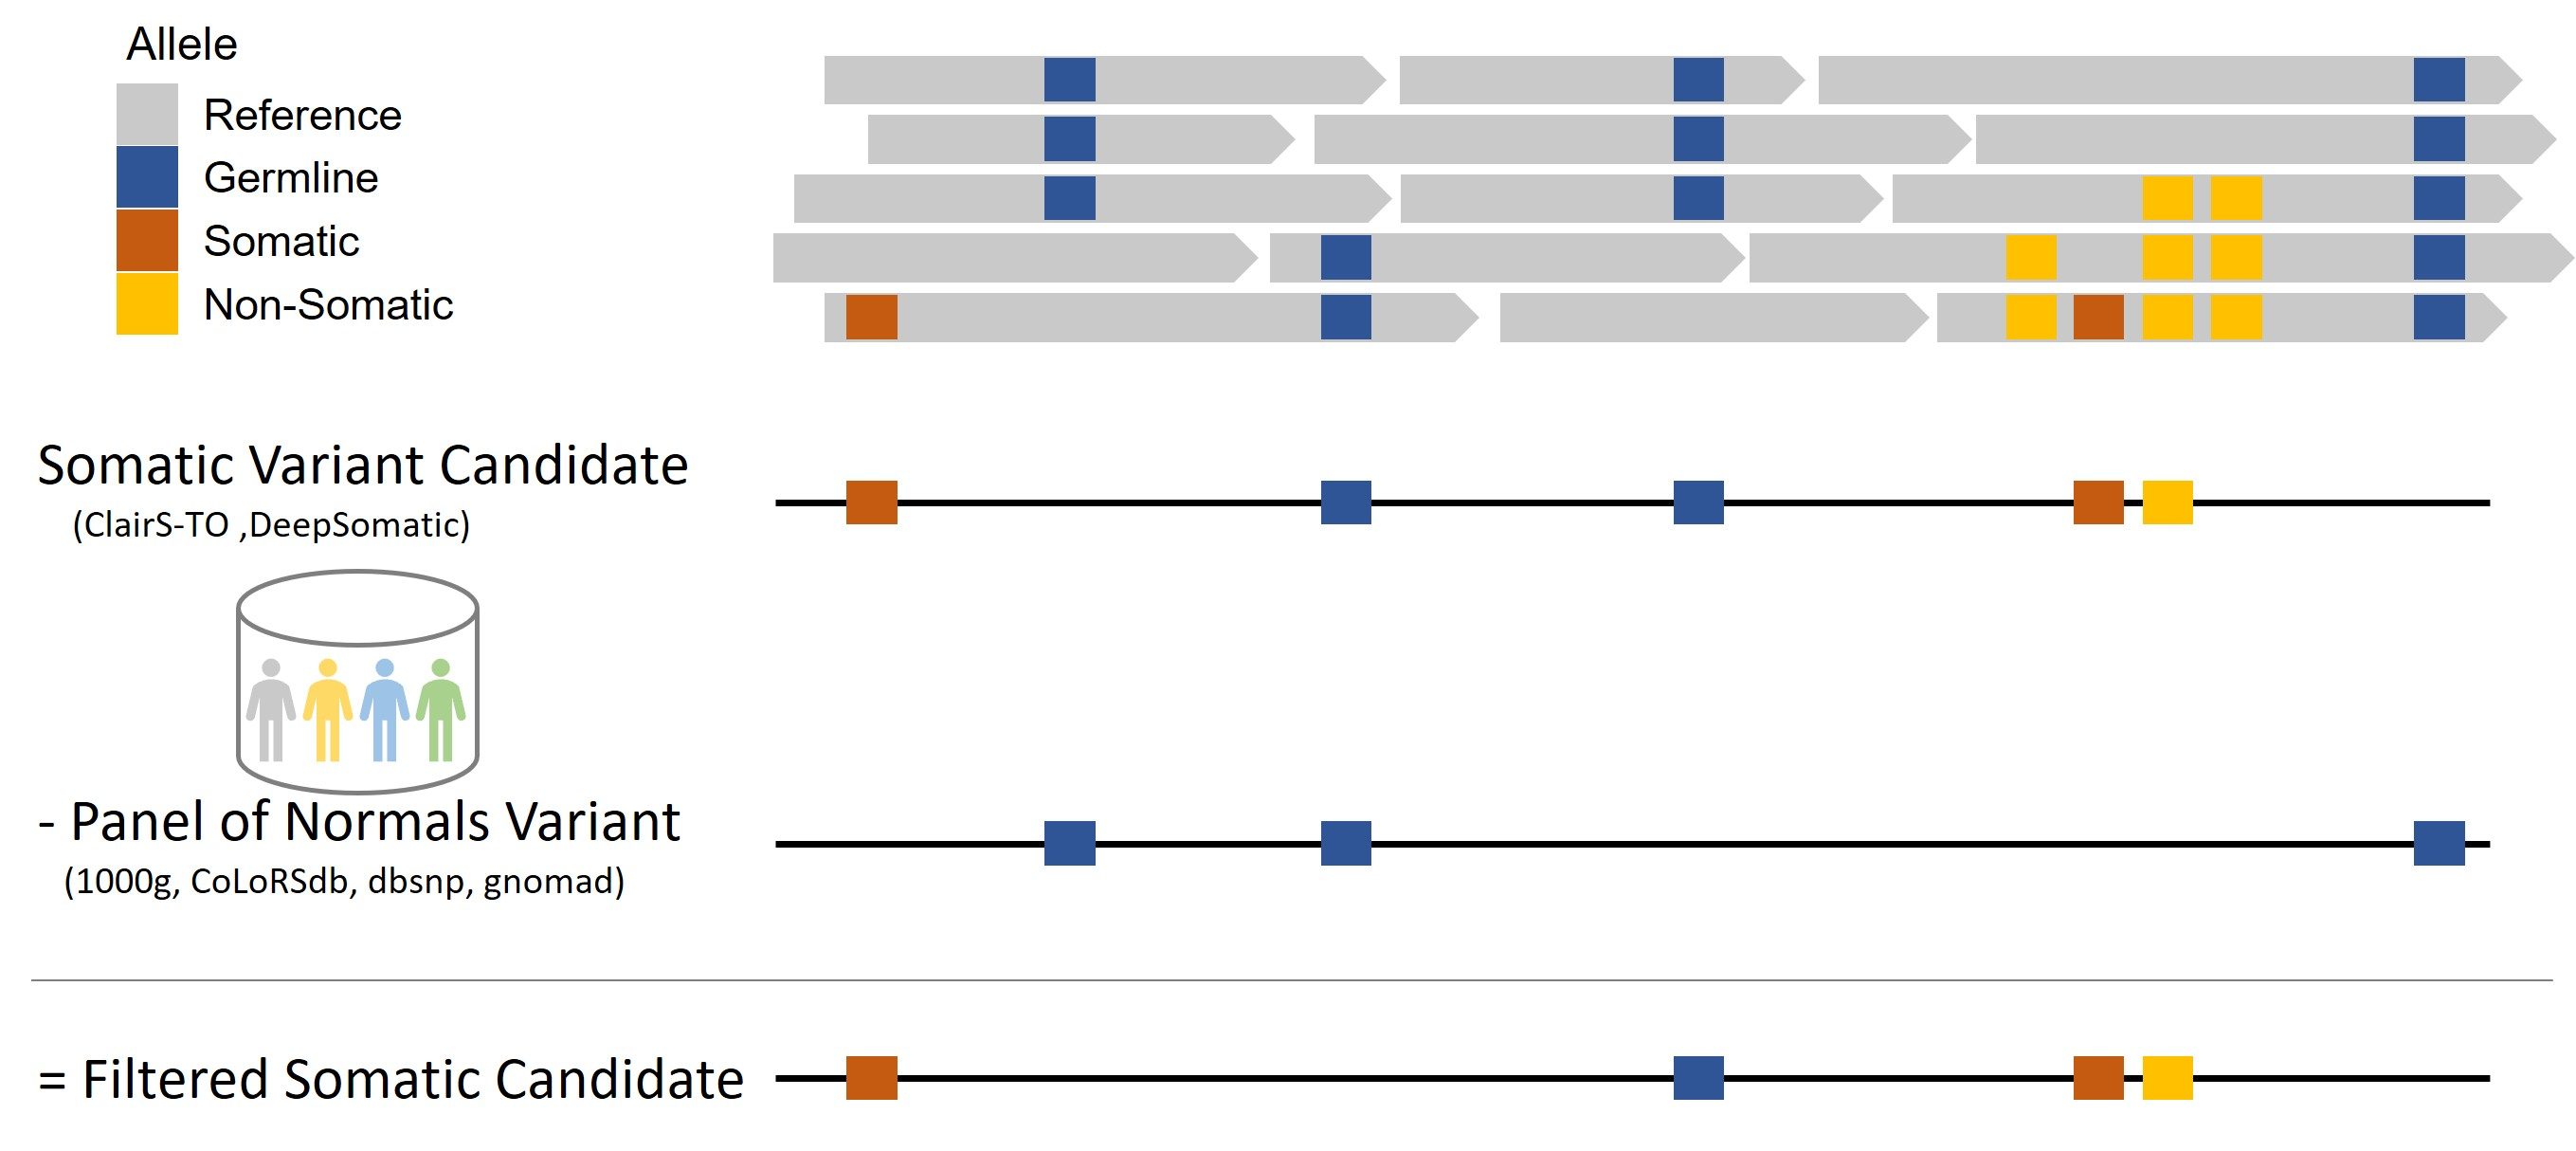
\includegraphics[width=0.8\textwidth,keepaspectratio]{page_18_cropped.jpg}}
%   \caption[Panel of Normals Filtering]{Filtering somatic variant candidates using a Panel of Normals (PoN). This schematic shows that an initial set of variant candidates, containing a mix of somatic (brown), germline (blue), and other variants, is filtered by subtracting all variants found in the PON. This process enriches the final candidate list for true somatic mutations by removing common germline polymorphisms and known artifacts.}\label{fig:met-page-18-cropped-jpg}
% \end{figure}

% \begin{figure}
%   \centering
%   \pandocbounded{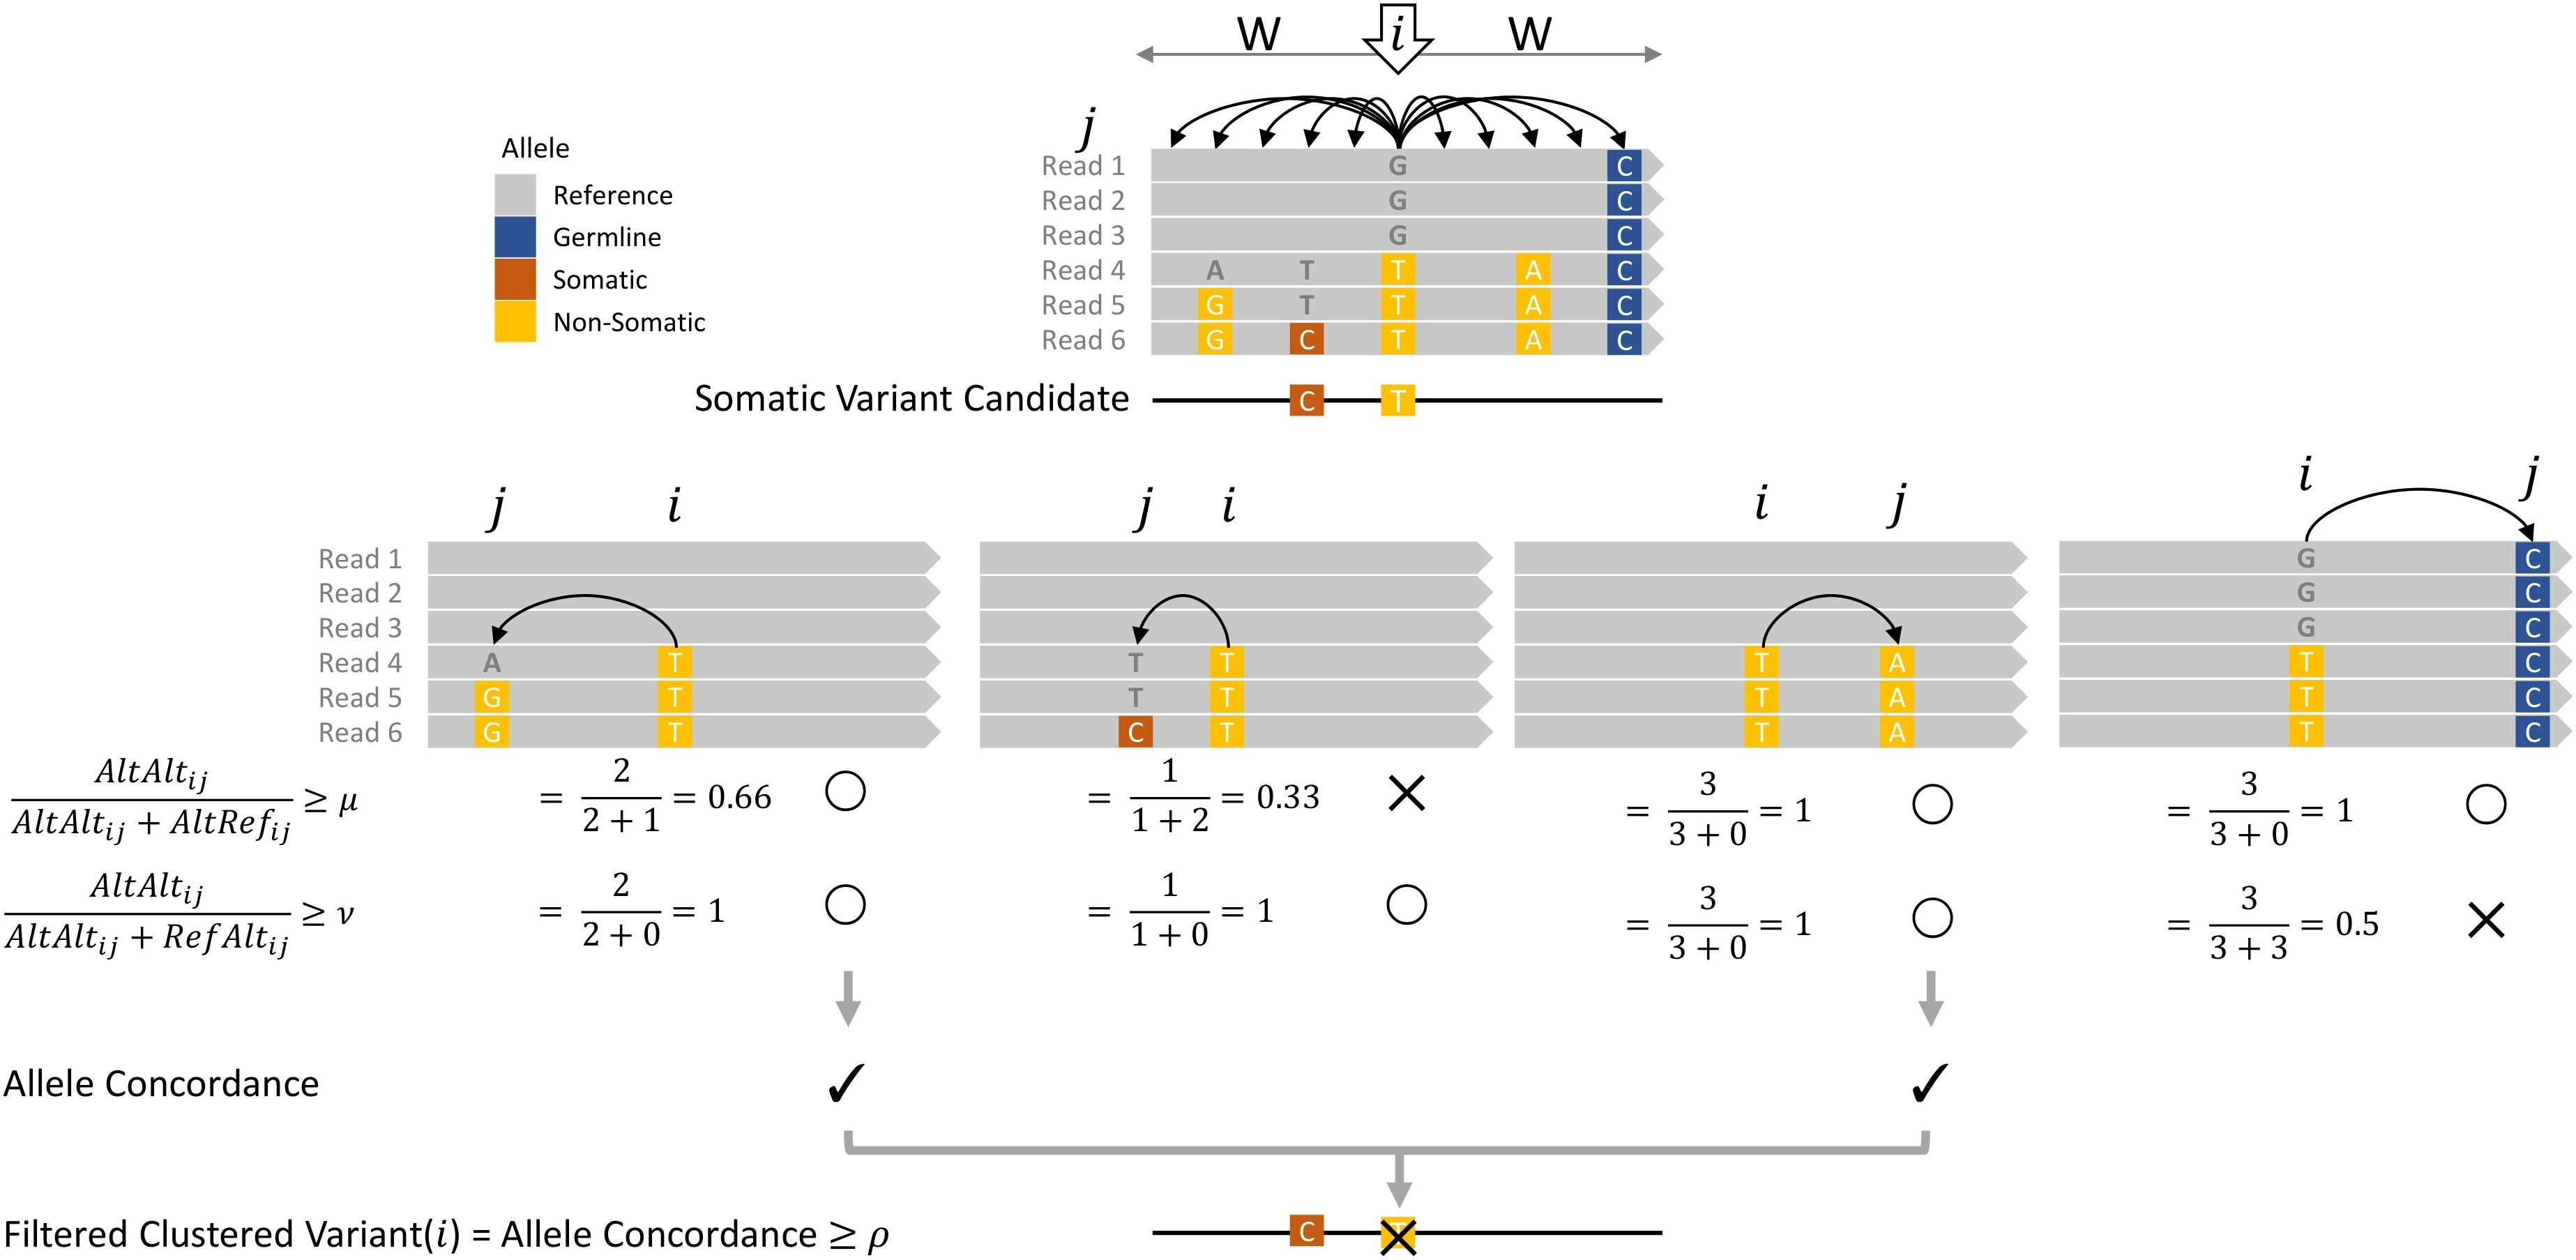
\includegraphics[keepaspectratio]{page_19_cropped.jpg}}
%   \caption[Allele concordance filtering]{Filtering clustered artifacts by allele concordance. For each candidate, non-reference mismatches within 100 aligned positions on either side are compared between reference- and alternate-supporting reads. A candidate is removed when at least two mismatches occur in at least 50\% of alternate-supporting reads and at least 60\% of all reads carrying the corresponding mismatch.}\label{fig:met-page-19-cropped-jpg}
% \end{figure}

% \begin{figure}
%   \centering
%   \pandocbounded{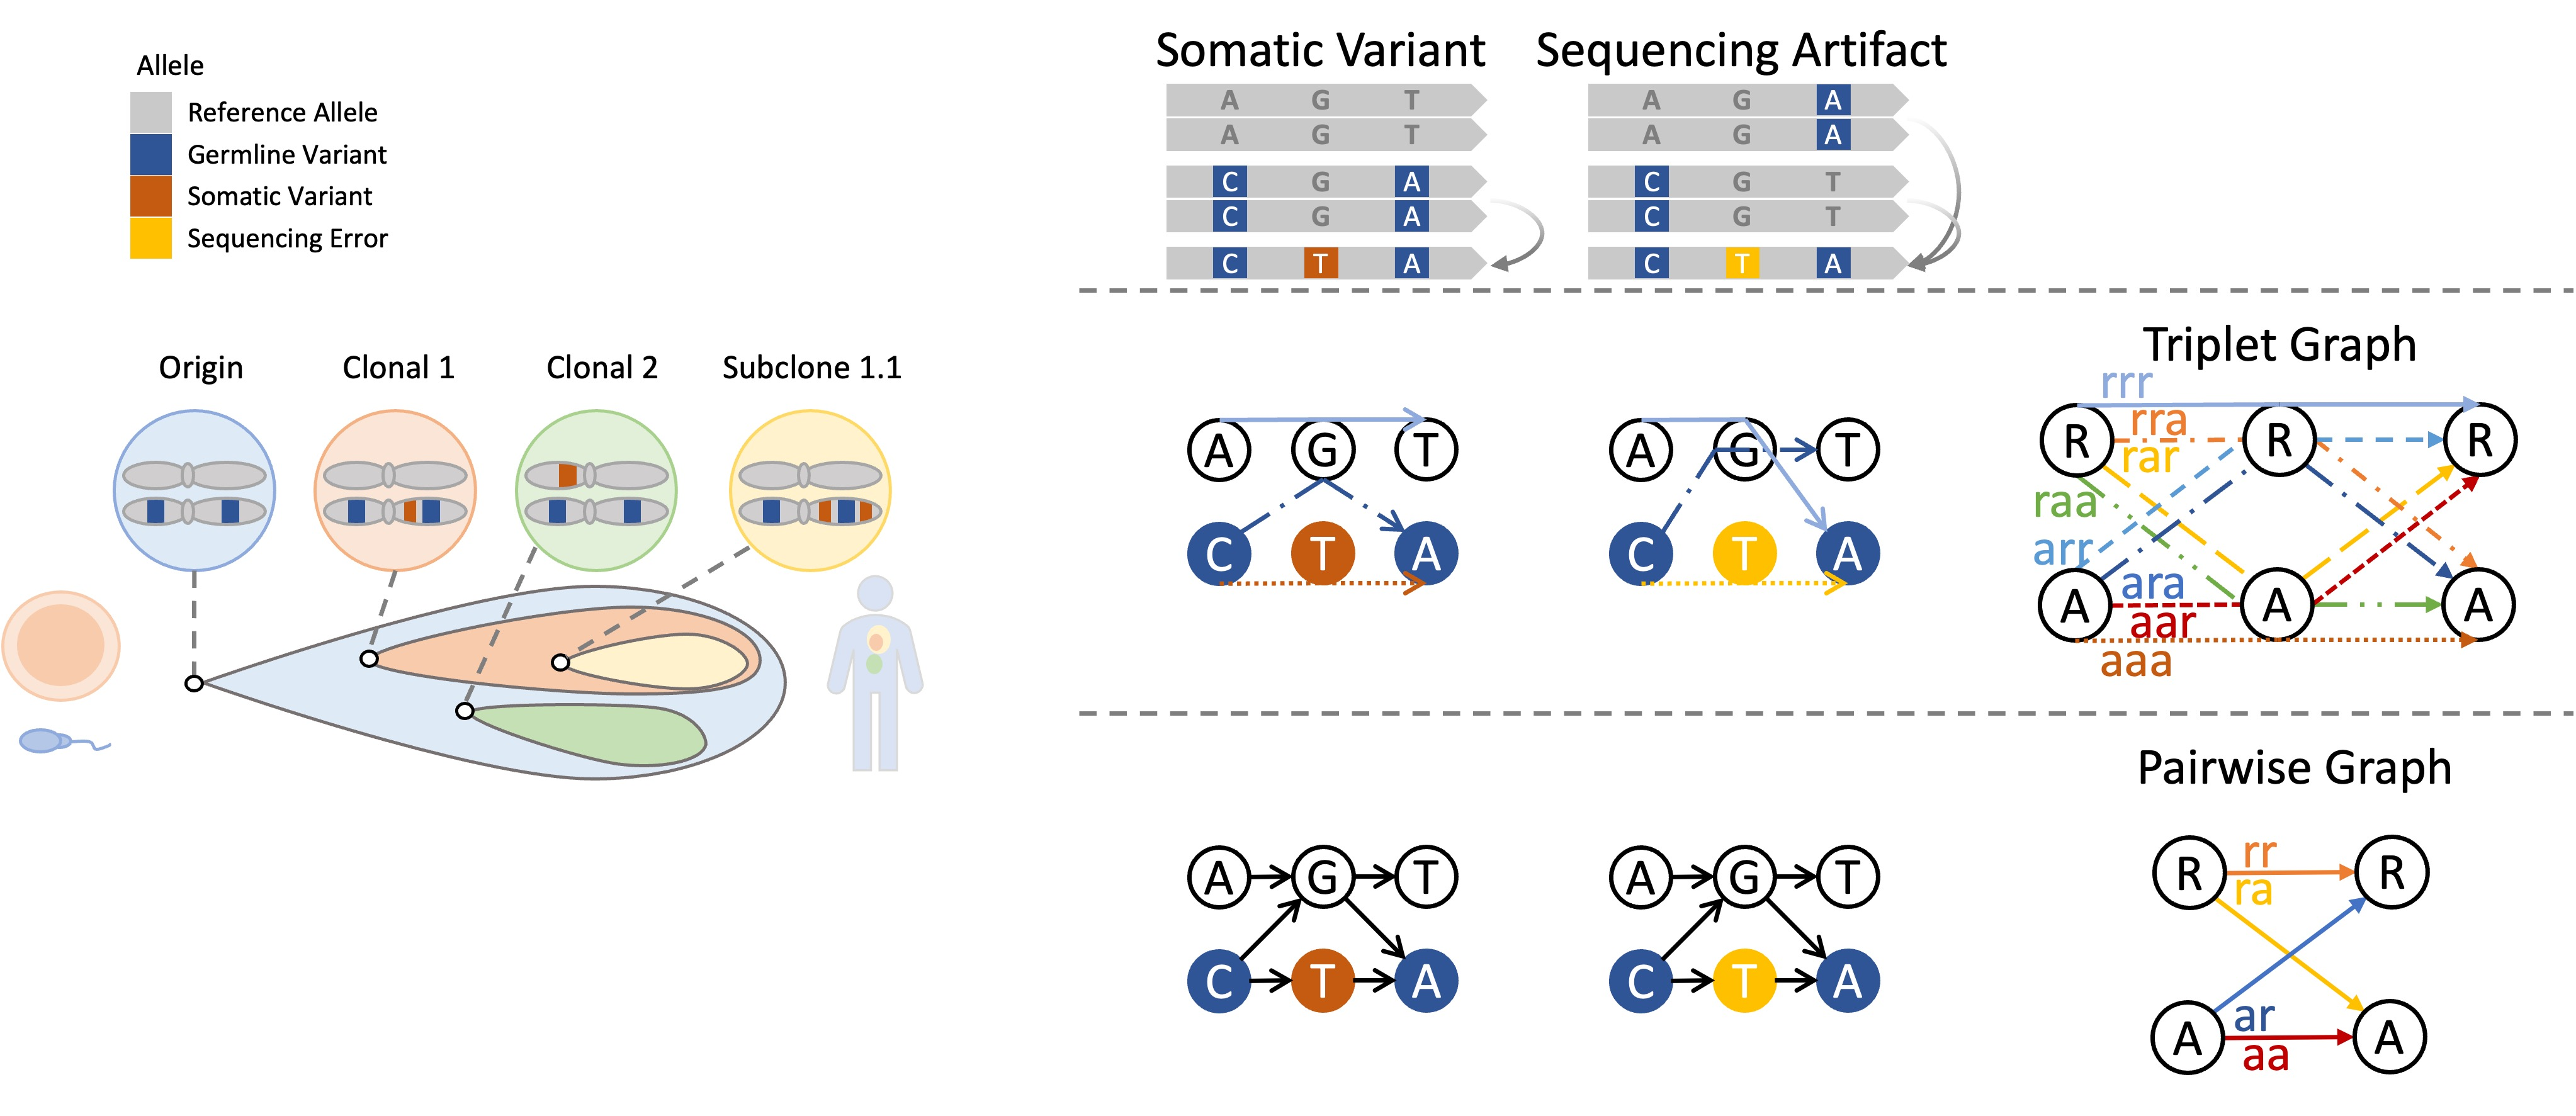
\includegraphics[keepaspectratio]{page_20_cropped.jpg}}
%   \caption[Graph Models Comparison]{Comparison of graph models for somatic variant recalibration. The figure contrasts the proposed triplet graph, which models haplotypes across three adjacent variant sites, with a simpler pairwise graph that only considers pairs. The triplet graph captures more linkage information, making it more powerful for distinguishing true somatic variants from artifacts, while the pairwise graph is labeled noninformative for this complex task.}\label{fig:met-page-20-cropped-jpg}
% \end{figure}

\begin{figure}
  \centering
  \pandocbounded{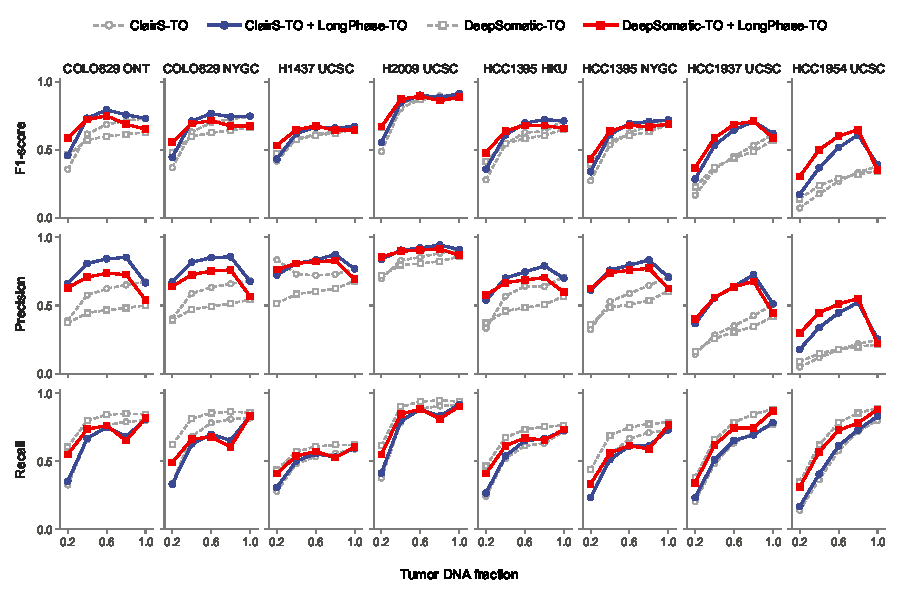
\includegraphics[width=\textwidth,keepaspectratio]{figures/supp_recal_ont_snv.pdf}}
  \caption[Somatic SNV recalibration on nanopore data]{Somatic SNV recalibration on nanopore data. F1-score, precision and recall of ClairS-TO and DeepSomatic-TO SNV calling, with LongPhase-TO recalibration (solid colored lines) and alone (gray dashed lines, open circles for ClairS-TO and open squares for DeepSomatic-TO), for the eight nanopore cell-line datasets across tumor DNA fractions from 20\% to 100\%. DeepSomatic-TO with LongPhase-TO uses the ClairS-TO normal panels. Per-mixture values are given in Supplementary Table~\ref{tab:somatic_purity}.}\label{fig:recal-ont-snv}
\end{figure}

\begin{figure}
  \centering
  \pandocbounded{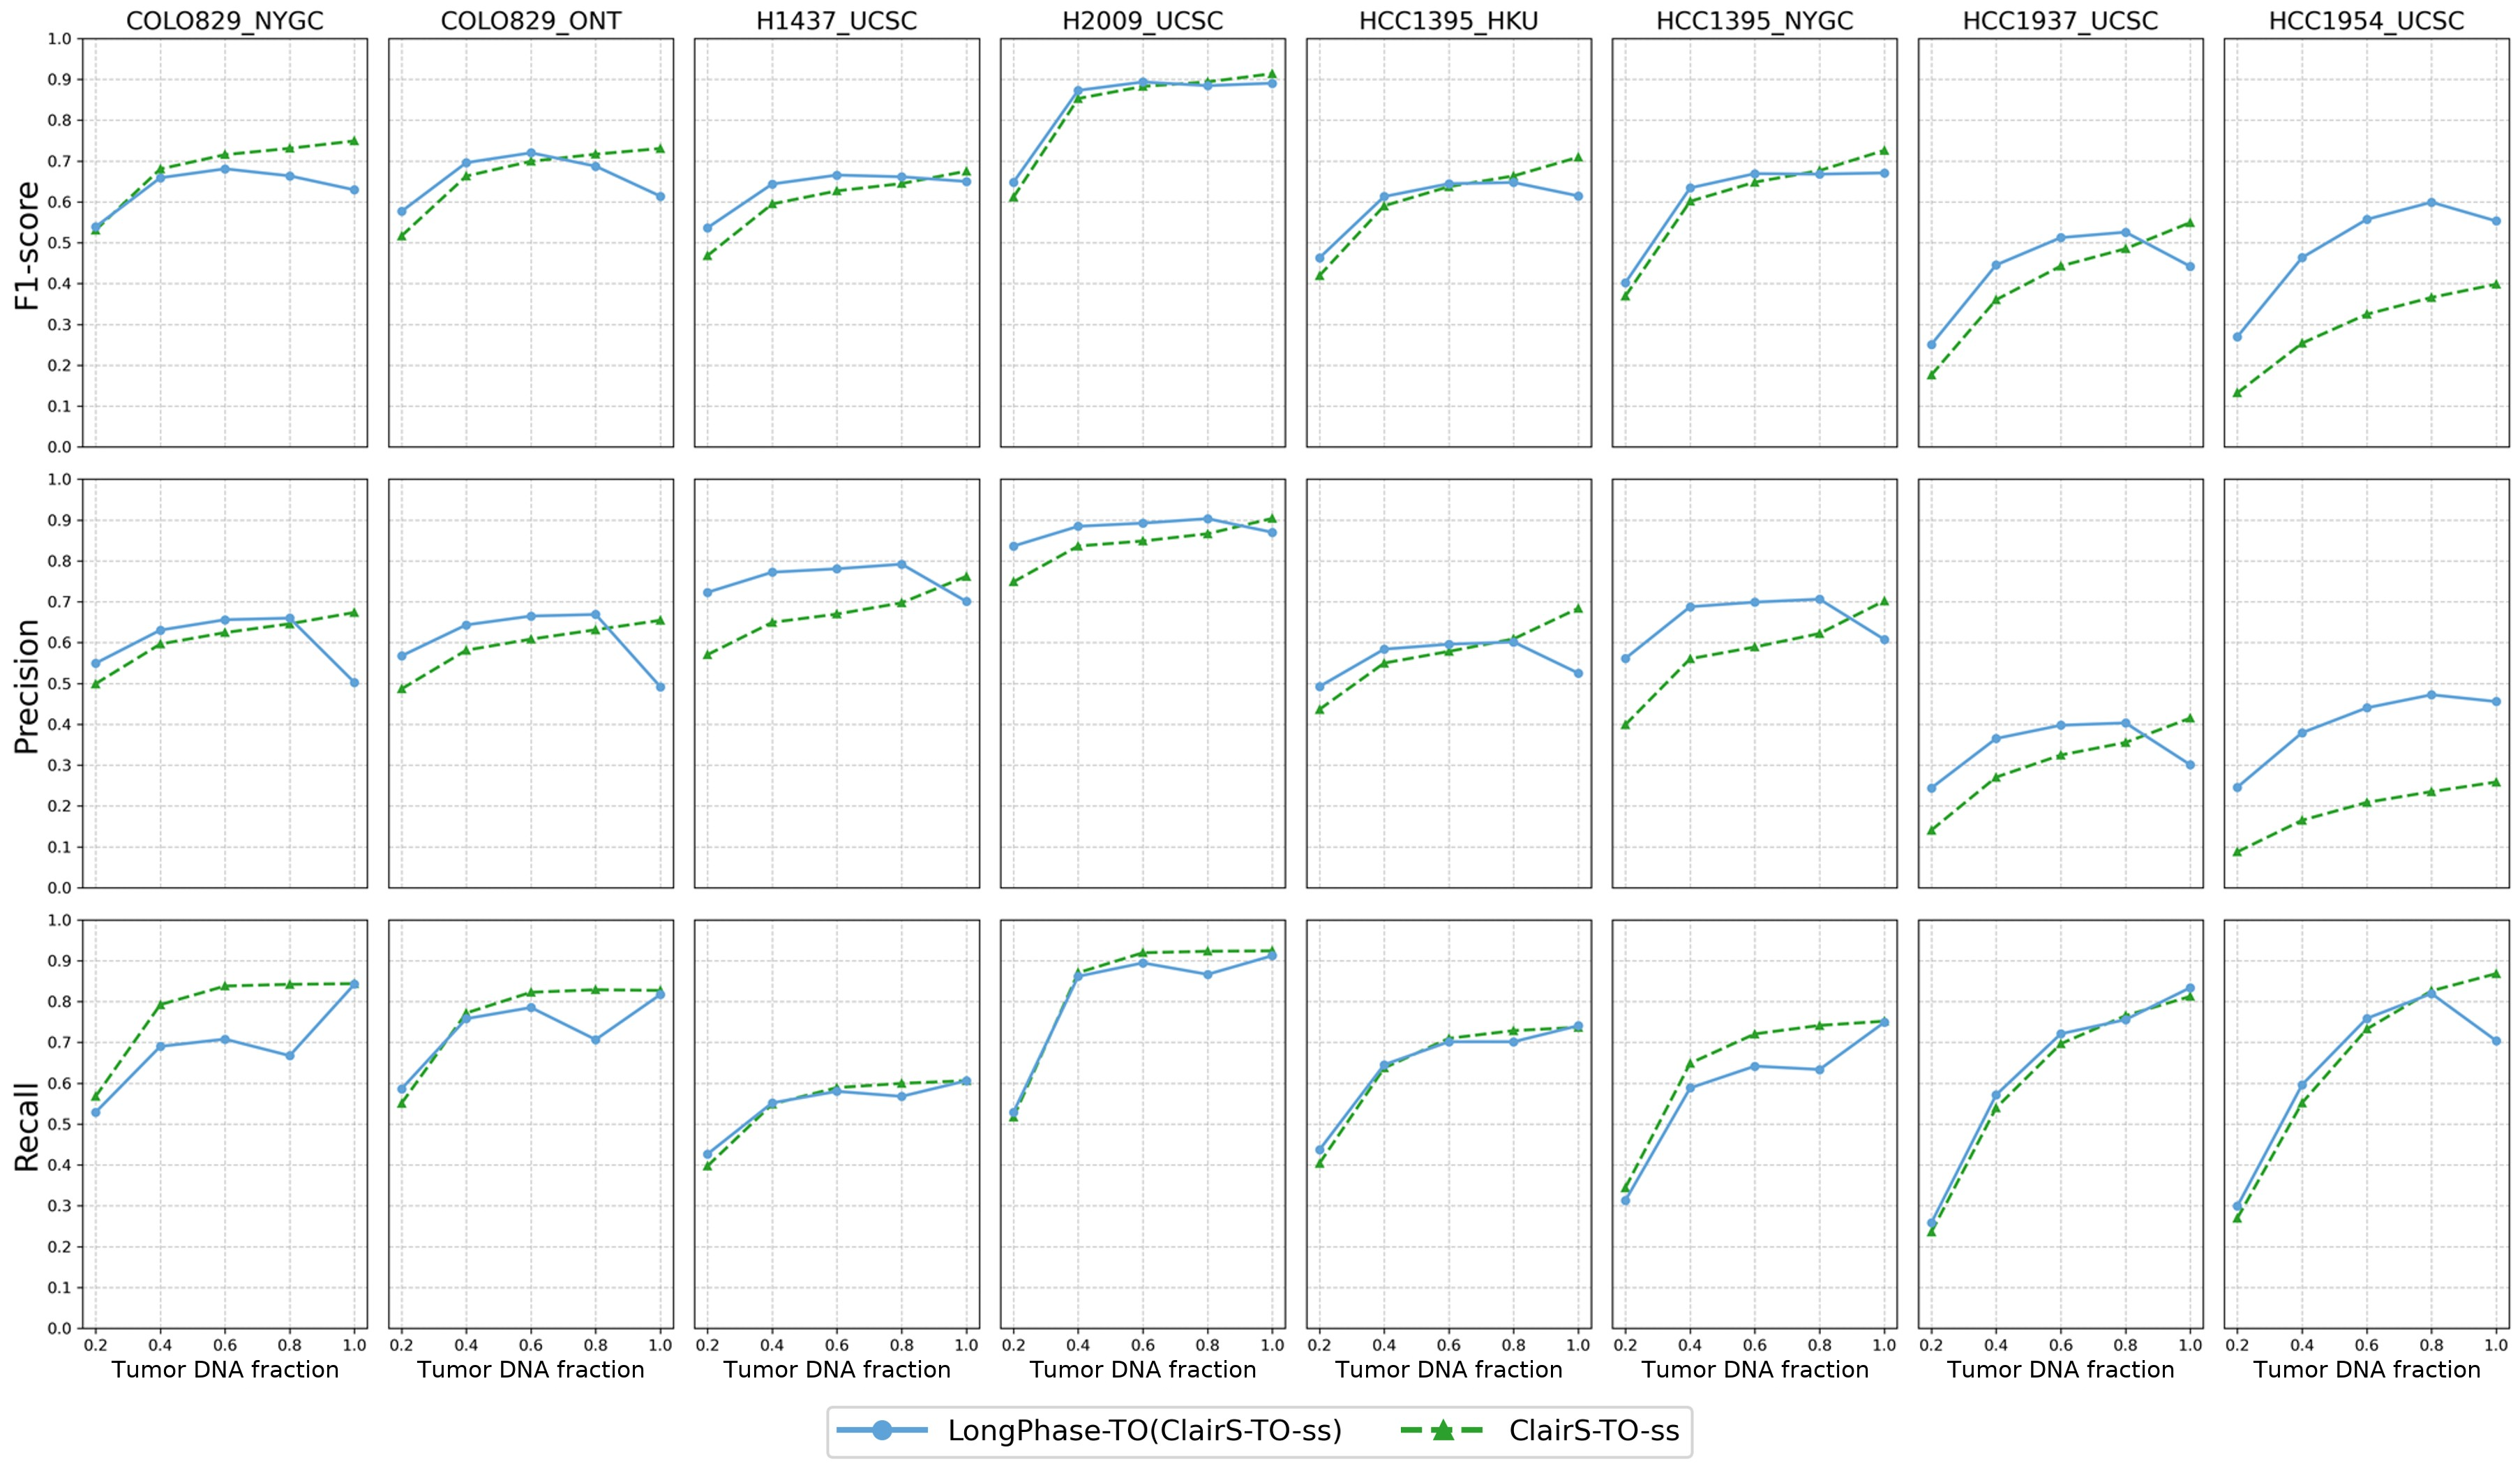
\includegraphics[keepaspectratio]{page_32_cropped_dnafraction.png}}
  \caption[Somatic variant calling performance of ClairS-TO-ss]{Somatic variant calling performance of ClairS-TO-ss with and without LongPhase-TO across eight cancer cell-line datasets at tumor DNA fractions from 20\% to 100\%. LongPhase-TO generally improved precision, while recall was reduced to varying degrees.}
  \label{fig:met-page-32-cropped-jpg}
\end{figure}

\begin{figure}
  \centering
  \pandocbounded{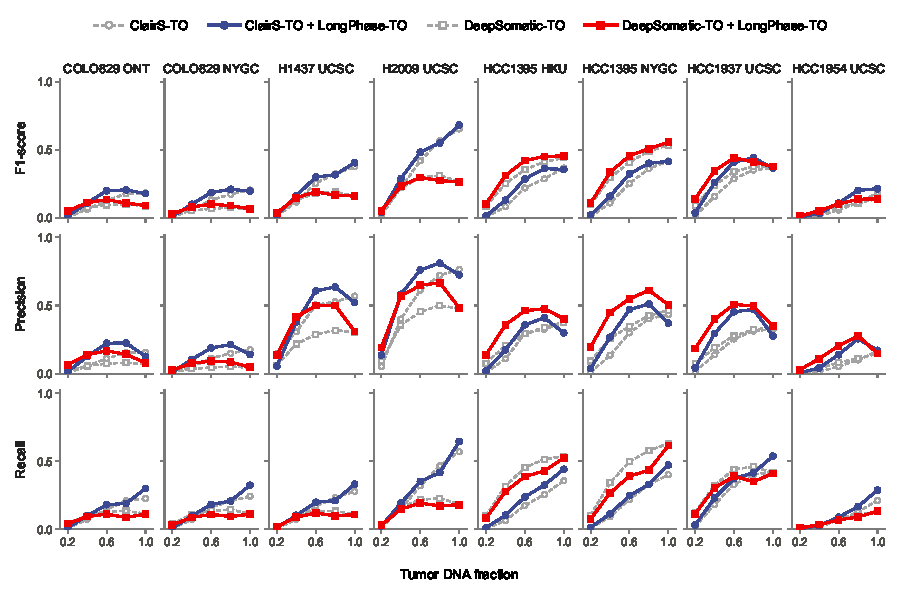
\includegraphics[width=\textwidth,keepaspectratio]{figures/supp_recal_ont_indel.pdf}}
  \caption[Somatic indel recalibration on nanopore data]{Somatic indel recalibration on nanopore data. F1-score, precision and recall of ClairS-TO and DeepSomatic-TO indel calling, with LongPhase-TO recalibration (solid colored lines) and alone (gray dashed lines, open circles for ClairS-TO and open squares for DeepSomatic-TO), for the eight nanopore cell-line datasets across tumor DNA fractions from 20\% to 100\%. DeepSomatic-TO with LongPhase-TO uses the ClairS-TO normal panels. Per-mixture values are given in Supplementary Table~\ref{tab:somatic_indel_purity}.}\label{fig:recal-ont-indel}
\end{figure}

\begin{figure}
  \centering
  \pandocbounded{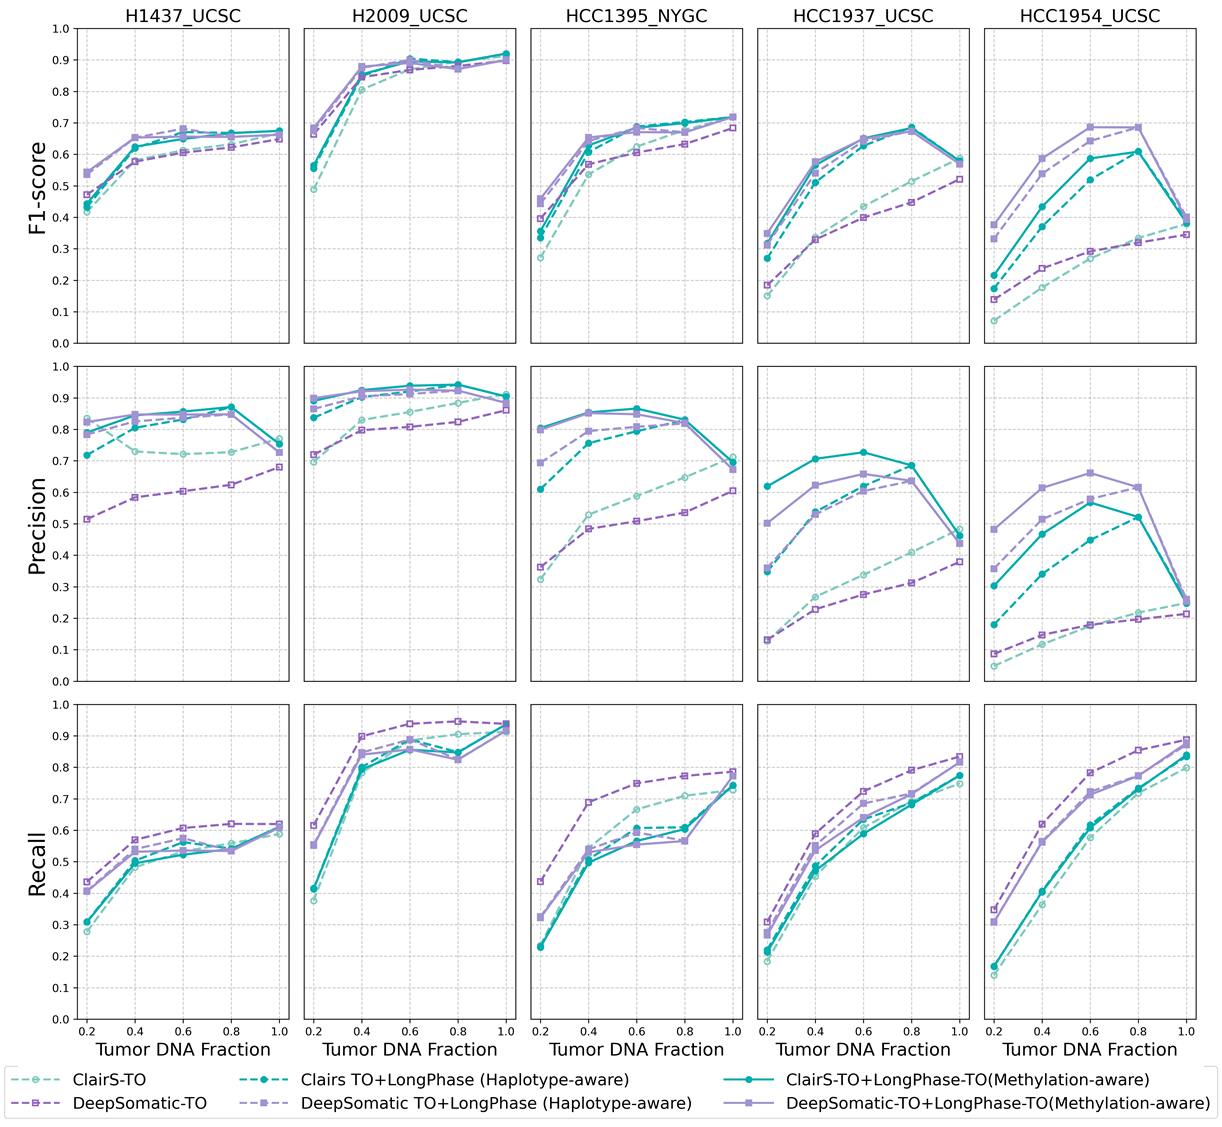
\includegraphics[width=\textwidth,keepaspectratio]{methylation_recalibration_snv.png}}
  \caption[Methylation-aware recalibration improves somatic SNV calling]{Methylation-aware recalibration improves somatic SNV calling beyond haplotype-aware recalibration alone. F1-score, precision and recall of ClairS-TO and DeepSomatic-TO SNV calling are shown for the five tumor cell-line datasets with 5-methylcytosine (5mC) tags available (H1437\_UCSC, H2009\_UCSC, HCC1395\_NYGC, HCC1937\_UCSC and HCC1954\_UCSC) across DNA fractions from 20\% to 100\%, comparing each caller alone, the caller after haplotype-aware (triplet-graph) recalibration, and the caller after the additional methylation-aware recalibration step. Averaged over the five datasets and both callers, the methylation-aware step raised mean SNV precision by 0.05 (0.68 to 0.72) at a mean recall cost of 0.01, giving a mean F1 gain of 0.01. Precision improved in 34 of the 50 caller-dataset-fraction combinations and declined in 2, with the largest gains in HCC1937\_UCSC (0.08) and HCC1954\_UCSC (0.07), the two datasets with the lowest haplotype-aware accuracy.}\label{fig:met-methylation-recalibration-snv}
\end{figure}

\begin{figure}
  \centering
  \pandocbounded{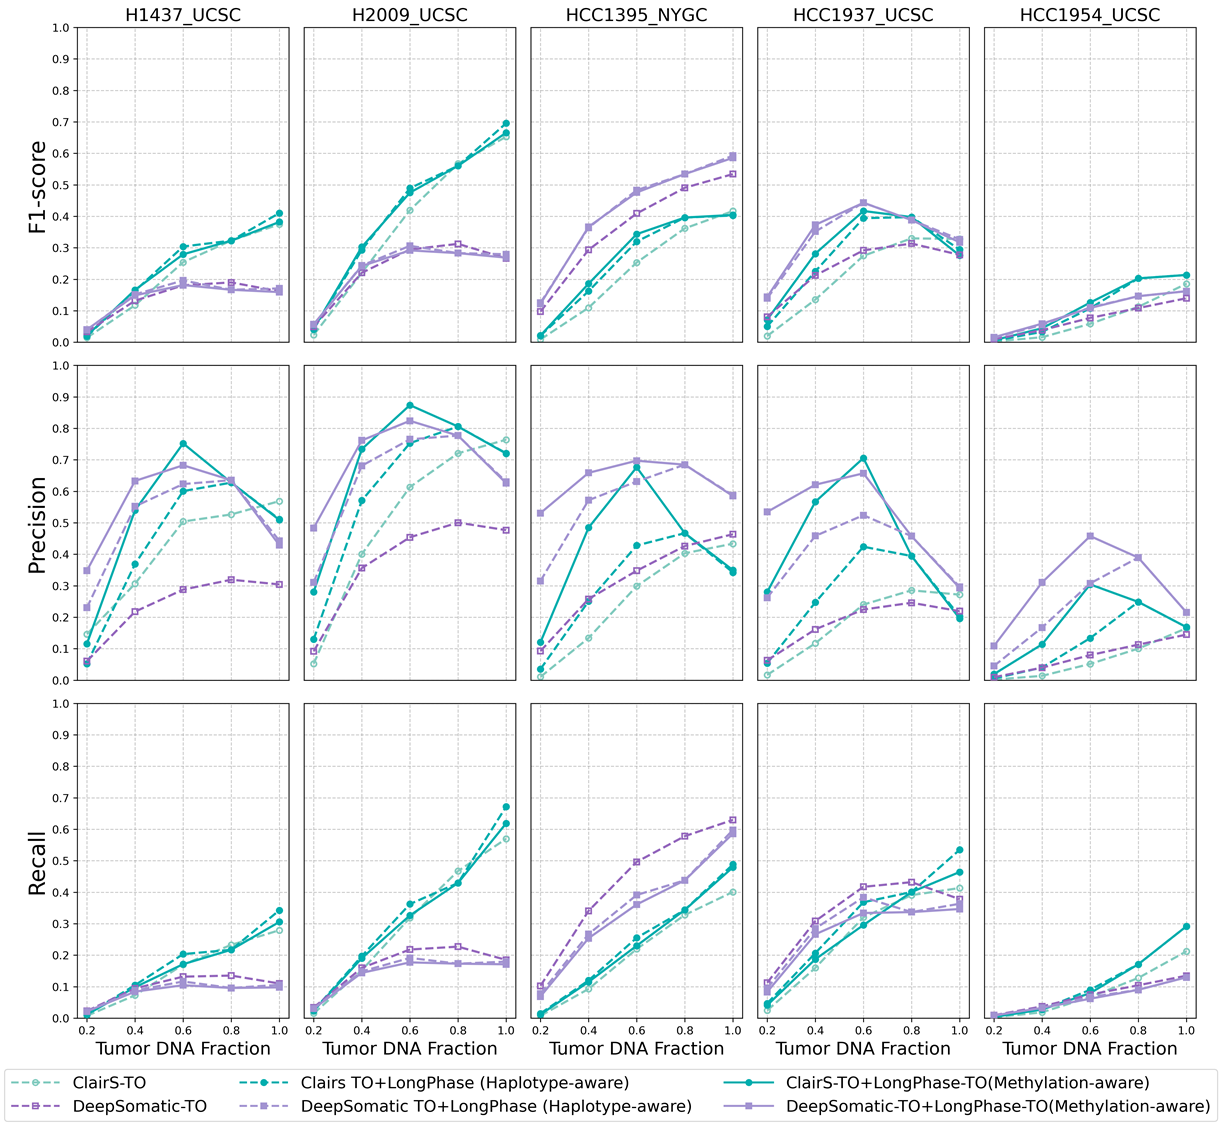
\includegraphics[width=\textwidth,keepaspectratio]{methylation_recalibration_indel.png}}
  \caption[Methylation-aware recalibration improves somatic indel precision]{Methylation-aware recalibration improves the precision of somatic indel calling beyond haplotype-aware recalibration alone. F1-score, precision and recall of ClairS-TO and DeepSomatic-TO indel calling are shown for the five tumor cell-line datasets with 5-methylcytosine (5mC) tags available (H1437\_UCSC, H2009\_UCSC, HCC1395\_NYGC, HCC1937\_UCSC and HCC1954\_UCSC) across DNA fractions from 20\% to 100\%, comparing each caller alone, the caller after haplotype-aware (triplet-graph) recalibration, and the caller after the additional methylation-aware recalibration step. Averaged over the five datasets and both callers, the methylation-aware step raised mean indel precision by 0.09 (0.40 to 0.49) at a mean recall cost of 0.01, leaving mean F1 essentially unchanged. Precision improved in 31 of the 50 caller-dataset-fraction combinations and declined in 7, with the largest gains in HCC1937\_UCSC (0.14) and HCC1395\_NYGC (0.09).}\label{fig:met-methylation-recalibration-indel}
\end{figure}

\begin{figure}
  \centering
  \pandocbounded{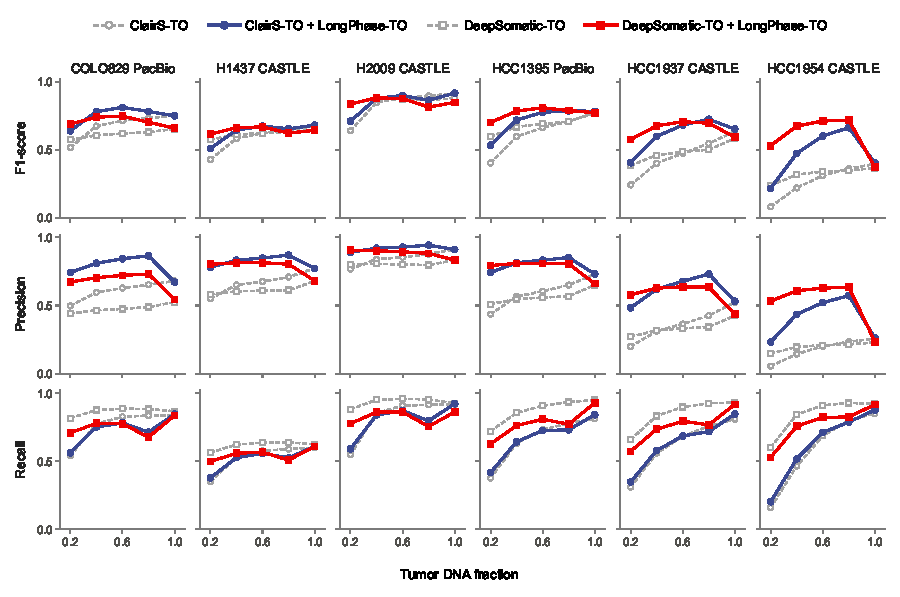
\includegraphics[width=\textwidth,keepaspectratio]{figures/supp_recal_pacbio_snv.pdf}}
  \caption[Somatic SNV recalibration transfers to PacBio HiFi]{Somatic SNV recalibration transfers to PacBio HiFi. F1-score, precision and recall of ClairS-TO and DeepSomatic-TO SNV calling, with LongPhase-TO recalibration (solid colored lines) and alone (gray dashed lines, open circles for ClairS-TO and open squares for DeepSomatic-TO), for the six PacBio HiFi cell-line datasets across tumor DNA fractions from 20\% to 100\%. DeepSomatic-TO with LongPhase-TO uses the ClairS-TO normal panels. Both callers were run with their PacBio HiFi models, whereas the triplet-graph coefficients and site-level thresholds were those fitted on nanopore data (HCC1395\_HKU at 0.6 tumor DNA fraction) and were applied without refitting. Recalibration raised mean SNV F1 from 0.58 to 0.67 for ClairS-TO and from 0.60 to 0.72 for DeepSomatic-TO, improving 28 and 26 of 30 points. Per-mixture values are given in Supplementary Table~\ref{tab:pacbio_somatic_snv}.}\label{fig:pacbio-snv-recalibration}
\end{figure}

\begin{figure}
  \centering
  \pandocbounded{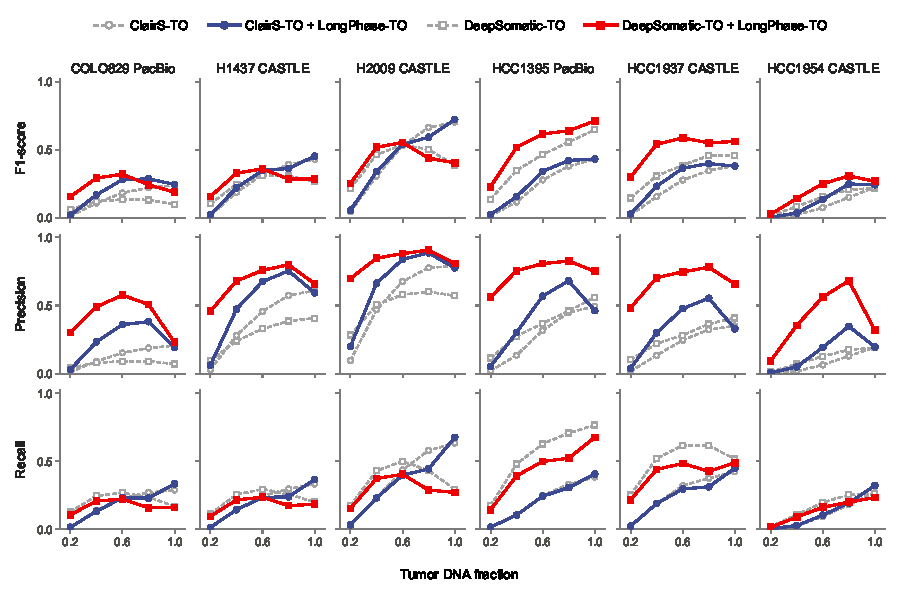
\includegraphics[width=\textwidth,keepaspectratio]{figures/supp_recal_pacbio_indel.pdf}}
  \caption[Somatic indel recalibration transfers to PacBio HiFi]{Somatic indel recalibration transfers to PacBio HiFi. F1-score, precision and recall of ClairS-TO and DeepSomatic-TO indel calling, with LongPhase-TO recalibration (solid colored lines) and alone (gray dashed lines, open circles for ClairS-TO and open squares for DeepSomatic-TO), for the six PacBio HiFi cell-line datasets across tumor DNA fractions from 20\% to 100\%. DeepSomatic-TO with LongPhase-TO uses the ClairS-TO normal panels. Both callers were run with their PacBio HiFi models, whereas the triplet-graph coefficients and site-level thresholds were those fitted on nanopore data (HCC1395\_HKU at 0.6 tumor DNA fraction) and were applied without refitting. Recalibration raised mean indel F1 from 0.24 to 0.27 for ClairS-TO and from 0.28 to 0.37 for DeepSomatic-TO, improving 27 and 28 of 30 points. Per-mixture values are given in Supplementary Table~\ref{tab:pacbio_somatic_indel}.}\label{fig:pacbio-indel-recalibration}
\end{figure}

\begin{figure}
  \centering
  \pandocbounded{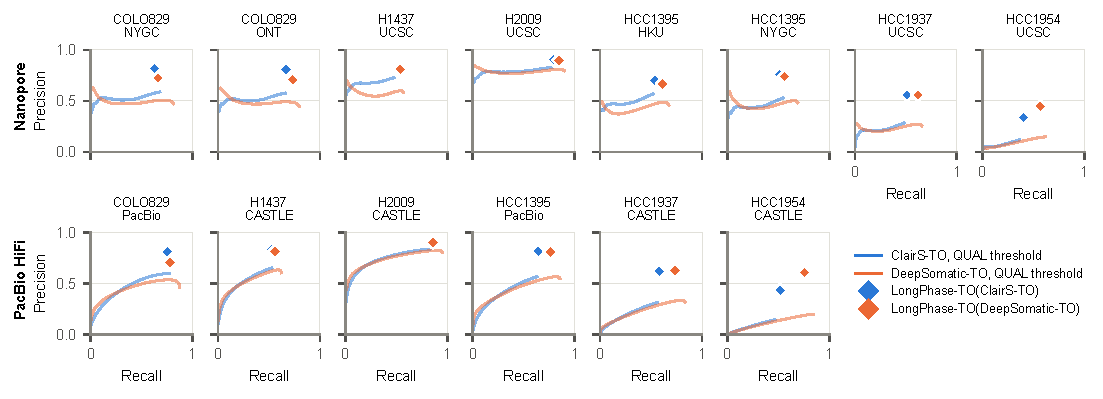
\includegraphics[width=\textwidth,keepaspectratio]{figures/supp_qual_threshold_pr.pdf}}
  \caption[LongPhase-TO compared with QUAL-threshold filtering]{LongPhase-TO compared with QUAL-threshold filtering of its input caller. Precision and recall of somatic SNVs at 0.4 tumor DNA fraction are shown for the eight nanopore (top) and six PacBio HiFi (bottom) cell-line datasets. Lines show ClairS-TO (blue) and DeepSomatic-TO (orange) when only the FILTER=PASS calls with QUAL at or above each of 50 thresholds are kept. The thresholds are the 0th to 98th percentiles of the QUAL values of the PASS calls. Diamonds show LongPhase-TO with the same caller as input. Nanopore HCC1937 uses the mixtures rebuilt from deduplicated reads. Results at the other DNA fractions and for indels are given in Supplementary Results (Section~\ref{supp:qual-threshold}).}\label{fig:qual-threshold-pr}
\end{figure}

\begin{figure}
  \centering
  \pandocbounded{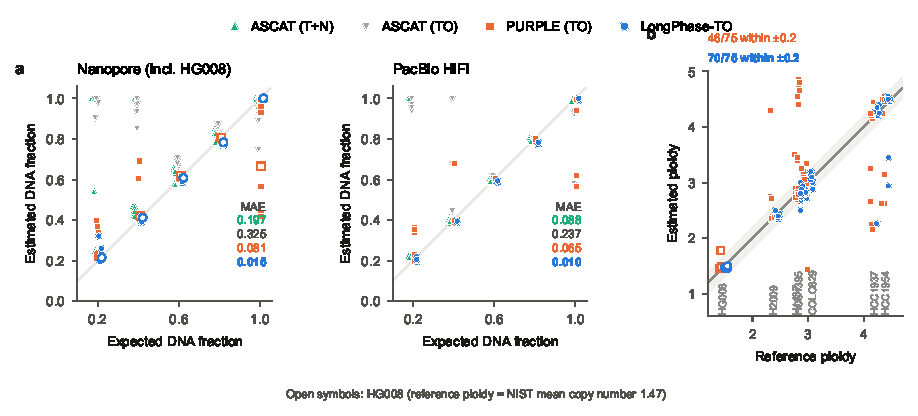
\includegraphics[width=\textwidth,keepaspectratio]{figures/supp_tdf_ploidy_by_platform.pdf}}
  \caption[Tumor DNA fraction and ploidy by sequencing platform]{Tumor DNA fraction and ploidy by sequencing platform. (a) Estimated against expected tumor DNA fraction for ASCAT (T+N), ASCAT (TO), PURPLE (TO) and LongPhase-TO. The nanopore panel shows the eight cell-line dilution series and the five HG008 mixtures (open symbols). The PacBio HiFi panel shows the six cell-line dilution series. ASCAT was not run on HG008. The diagonal indicates the ideal prediction ($y=x$), and the numbers give the mean absolute error of each method on that platform. ASCAT and PURPLE purities were converted to DNA fraction with each tool's fitted ploidy. (b) Estimated against reference ploidy for PURPLE (TO) and LongPhase-TO in all 75 runs of both platforms. The reference is the published ploidy of each cell line and the NIST mean total copy number (1.47) for HG008. The line and band mark the reference $\pm 0.2$. LongPhase-TO values are from the DeepSomatic-TO configuration with the ClairS-TO normal panels. Per-mixture values are given in Supplementary Tables~\ref{tab:tumor-purity}, \ref{tab:pacbio-tumor-purity}, \ref{tab:ploidy-accuracy} and~\ref{tab:hg008}.}\label{fig:pacbio-tdf}
\end{figure}

\begin{figure}
  \centering
  \pandocbounded{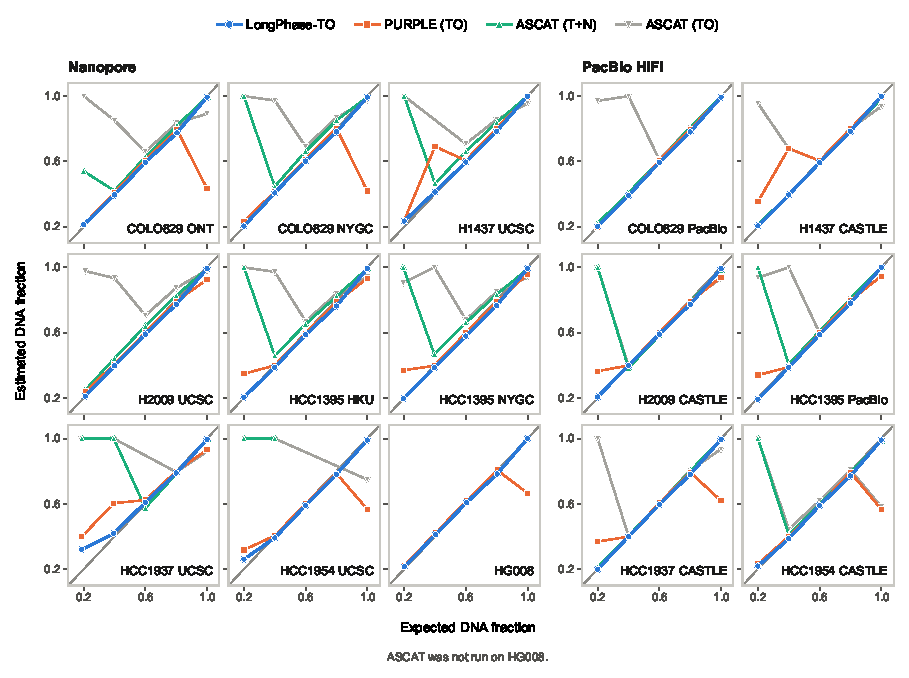
\includegraphics[width=\textwidth,keepaspectratio]{figures/supp_tdf_per_dataset.pdf}}
  \caption[Tumor DNA fraction of each dataset]{Tumor DNA fraction of each dataset. Each panel shows the estimated against the expected tumor DNA fraction of one dataset for ASCAT (T+N), ASCAT (TO), PURPLE (TO) and LongPhase-TO. The left block shows the nine nanopore datasets (eight cell-line dilution series and the five HG008 mixtures), and the right block shows the six PacBio HiFi cell-line dilution series. The COLO829 and HCC1395 replicates from different sequencing centers are shown in separate panels. ASCAT was not run on HG008. The diagonal indicates the ideal prediction ($y=x$). ASCAT and PURPLE purities were converted to DNA fraction with each tool's fitted ploidy. LongPhase-TO values are from the DeepSomatic-TO configuration with the ClairS-TO normal panels. Per-mixture values are given in Supplementary Tables~\ref{tab:tumor-purity}, \ref{tab:pacbio-tumor-purity} and~\ref{tab:hg008}.}\label{fig:tdf-per-dataset}
\end{figure}

\begin{figure}
  \centering
  \pandocbounded{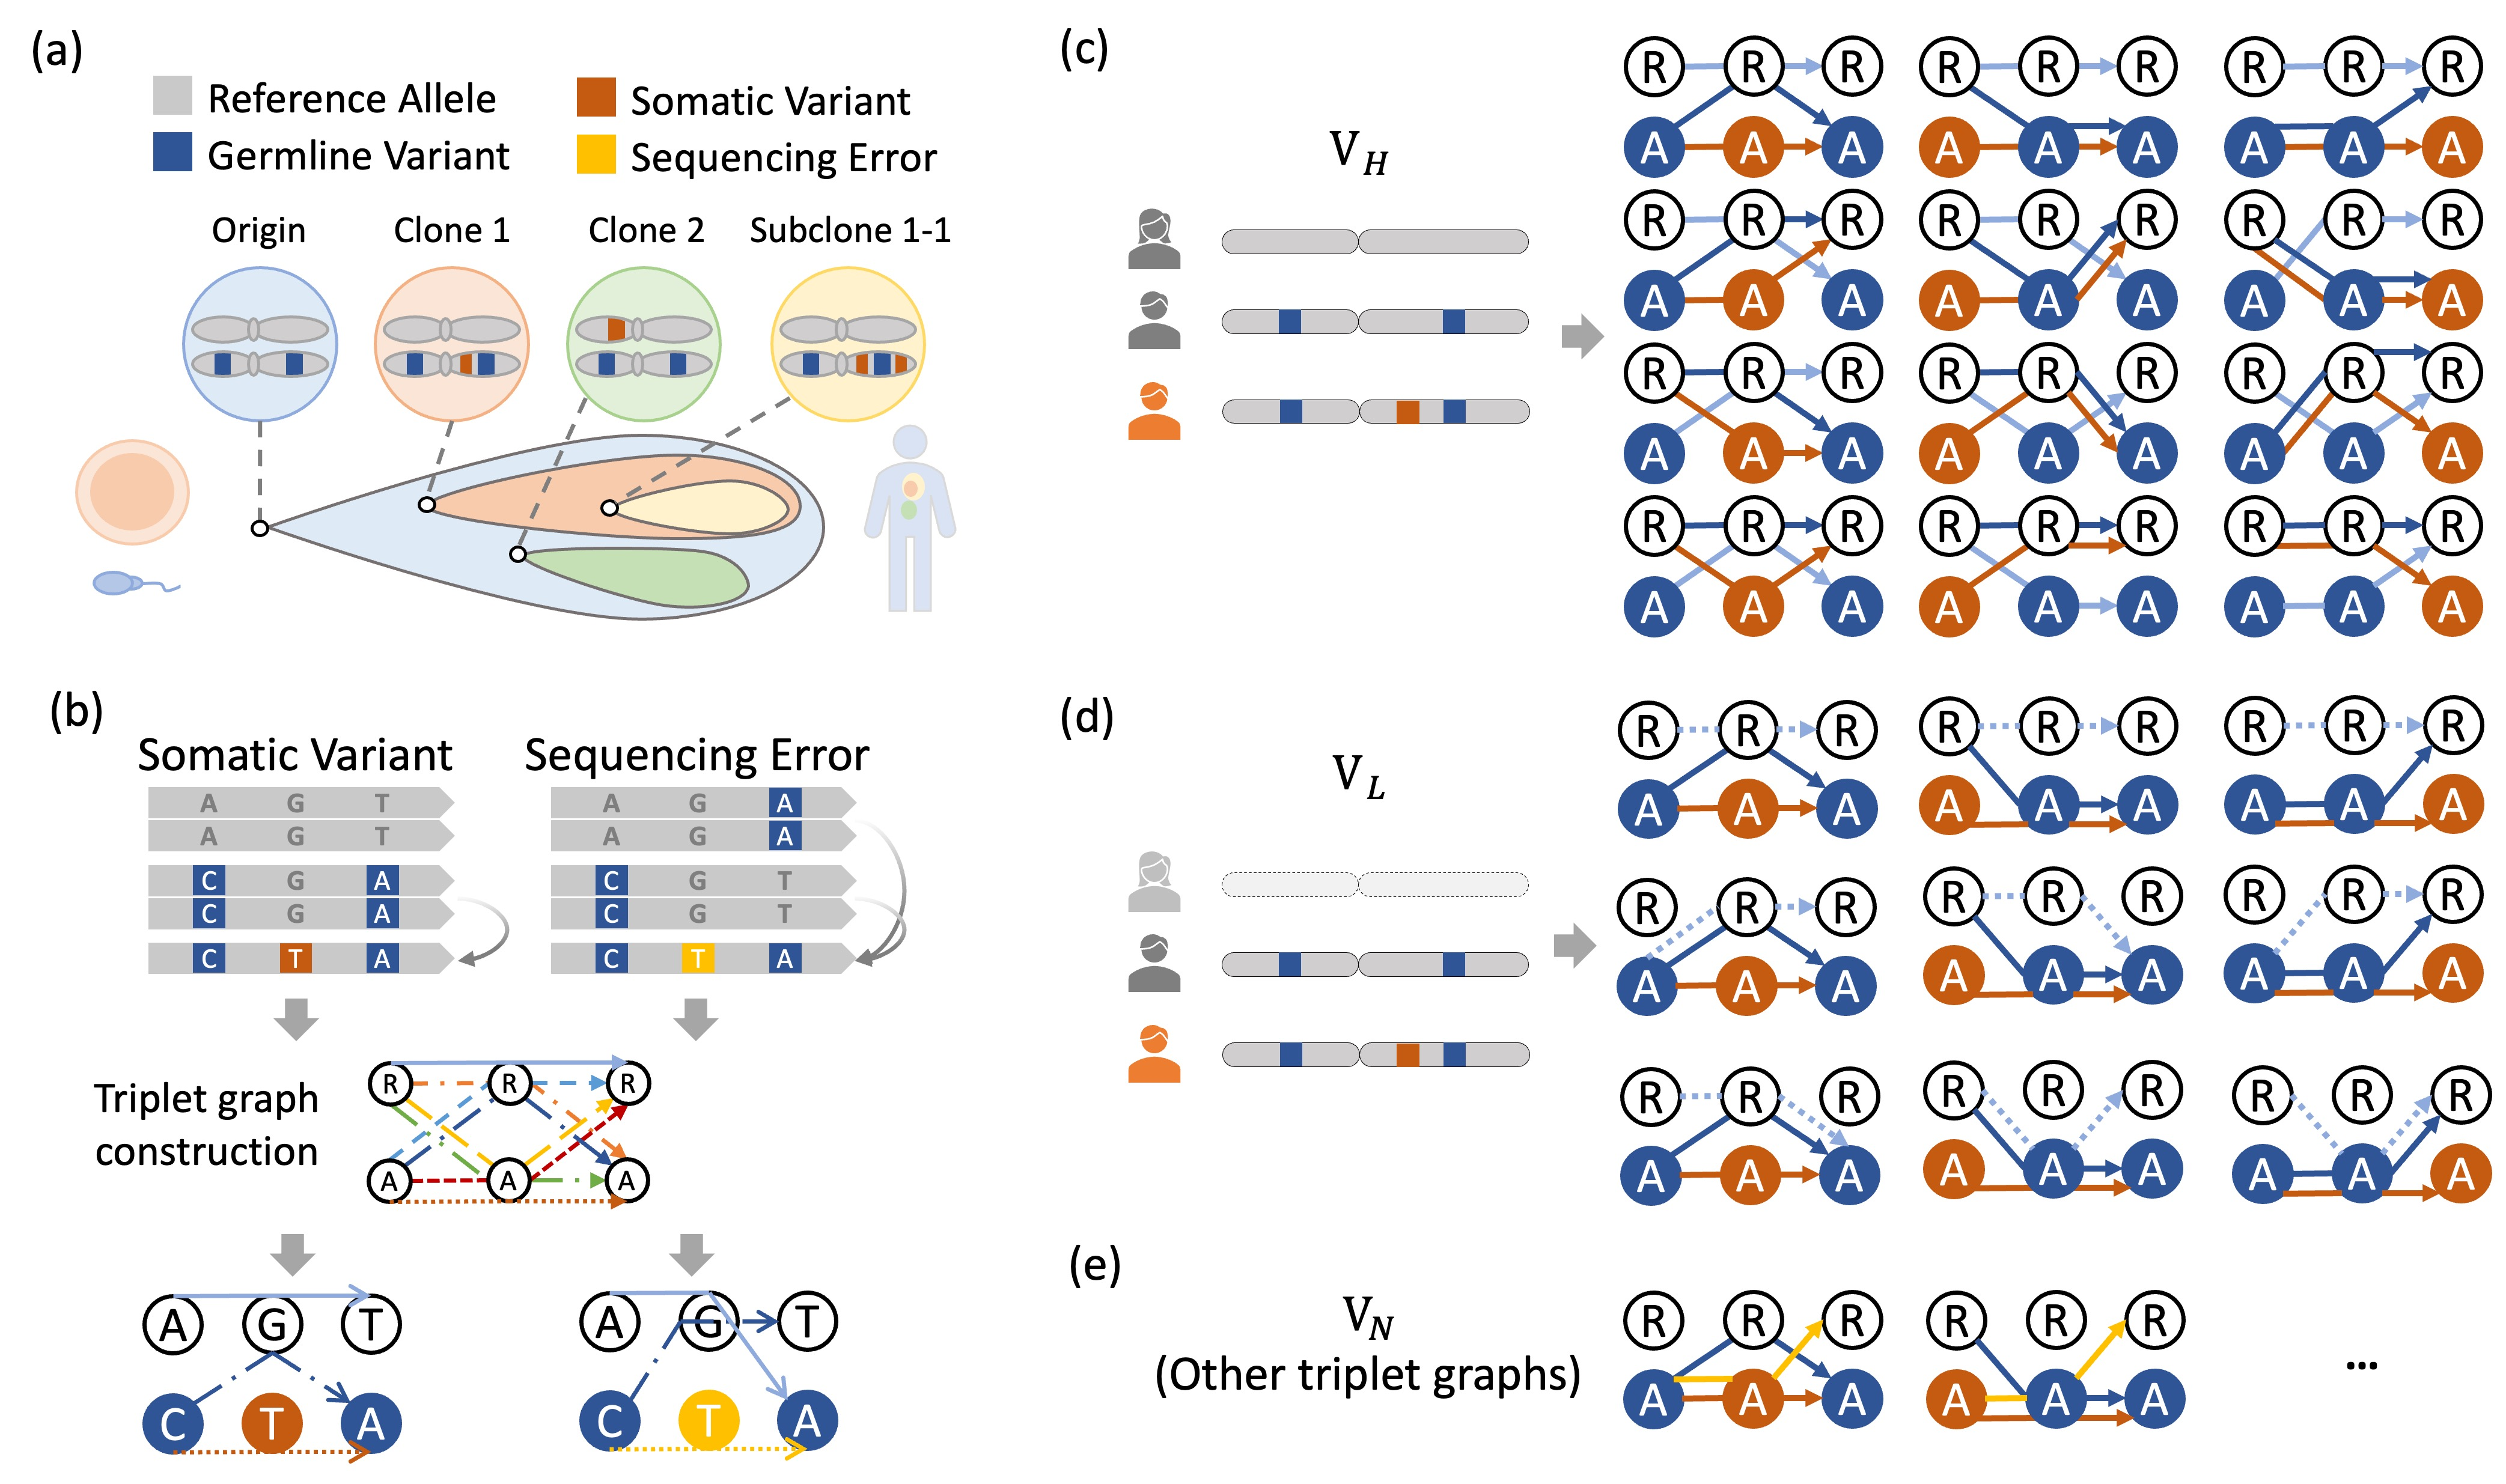
\includegraphics[keepaspectratio]{page_21_cropped.jpg}}
  \caption[Triplet-graph pattern classification]{Triplet-graph construction and pattern classification. (a) A somatic allele arises on one parental haplotype and is inherited through clonal evolution. (b) Reads spanning three adjacent variant positions define a triplet graph containing up to eight reference/alternate haplotype paths, and the examples contrast the consistent haplotype linkage of a somatic variant with the discordant linkage of a sequencing error. (c) The 12 high-confidence ($V_H$) configurations comprise four evolutionary configurations for each candidate position (middle, left and right columns), each containing two parental germline paths and one somatic-descendant path. (d) The nine lower-confidence ($V_L$) configurations comprise three candidate positions crossed with three permitted weak third paths: RRR and two paths that bypass the candidate alternate allele. (e) Sufficiently supported topologies classified as neither $V_H$ nor $V_L$ contribute a $V_N$ vote, and triplets with insufficient support do not vote.}\label{fig:met-page-21-cropped-jpg}
\end{figure}

\begin{figure}
  \centering
  \pandocbounded{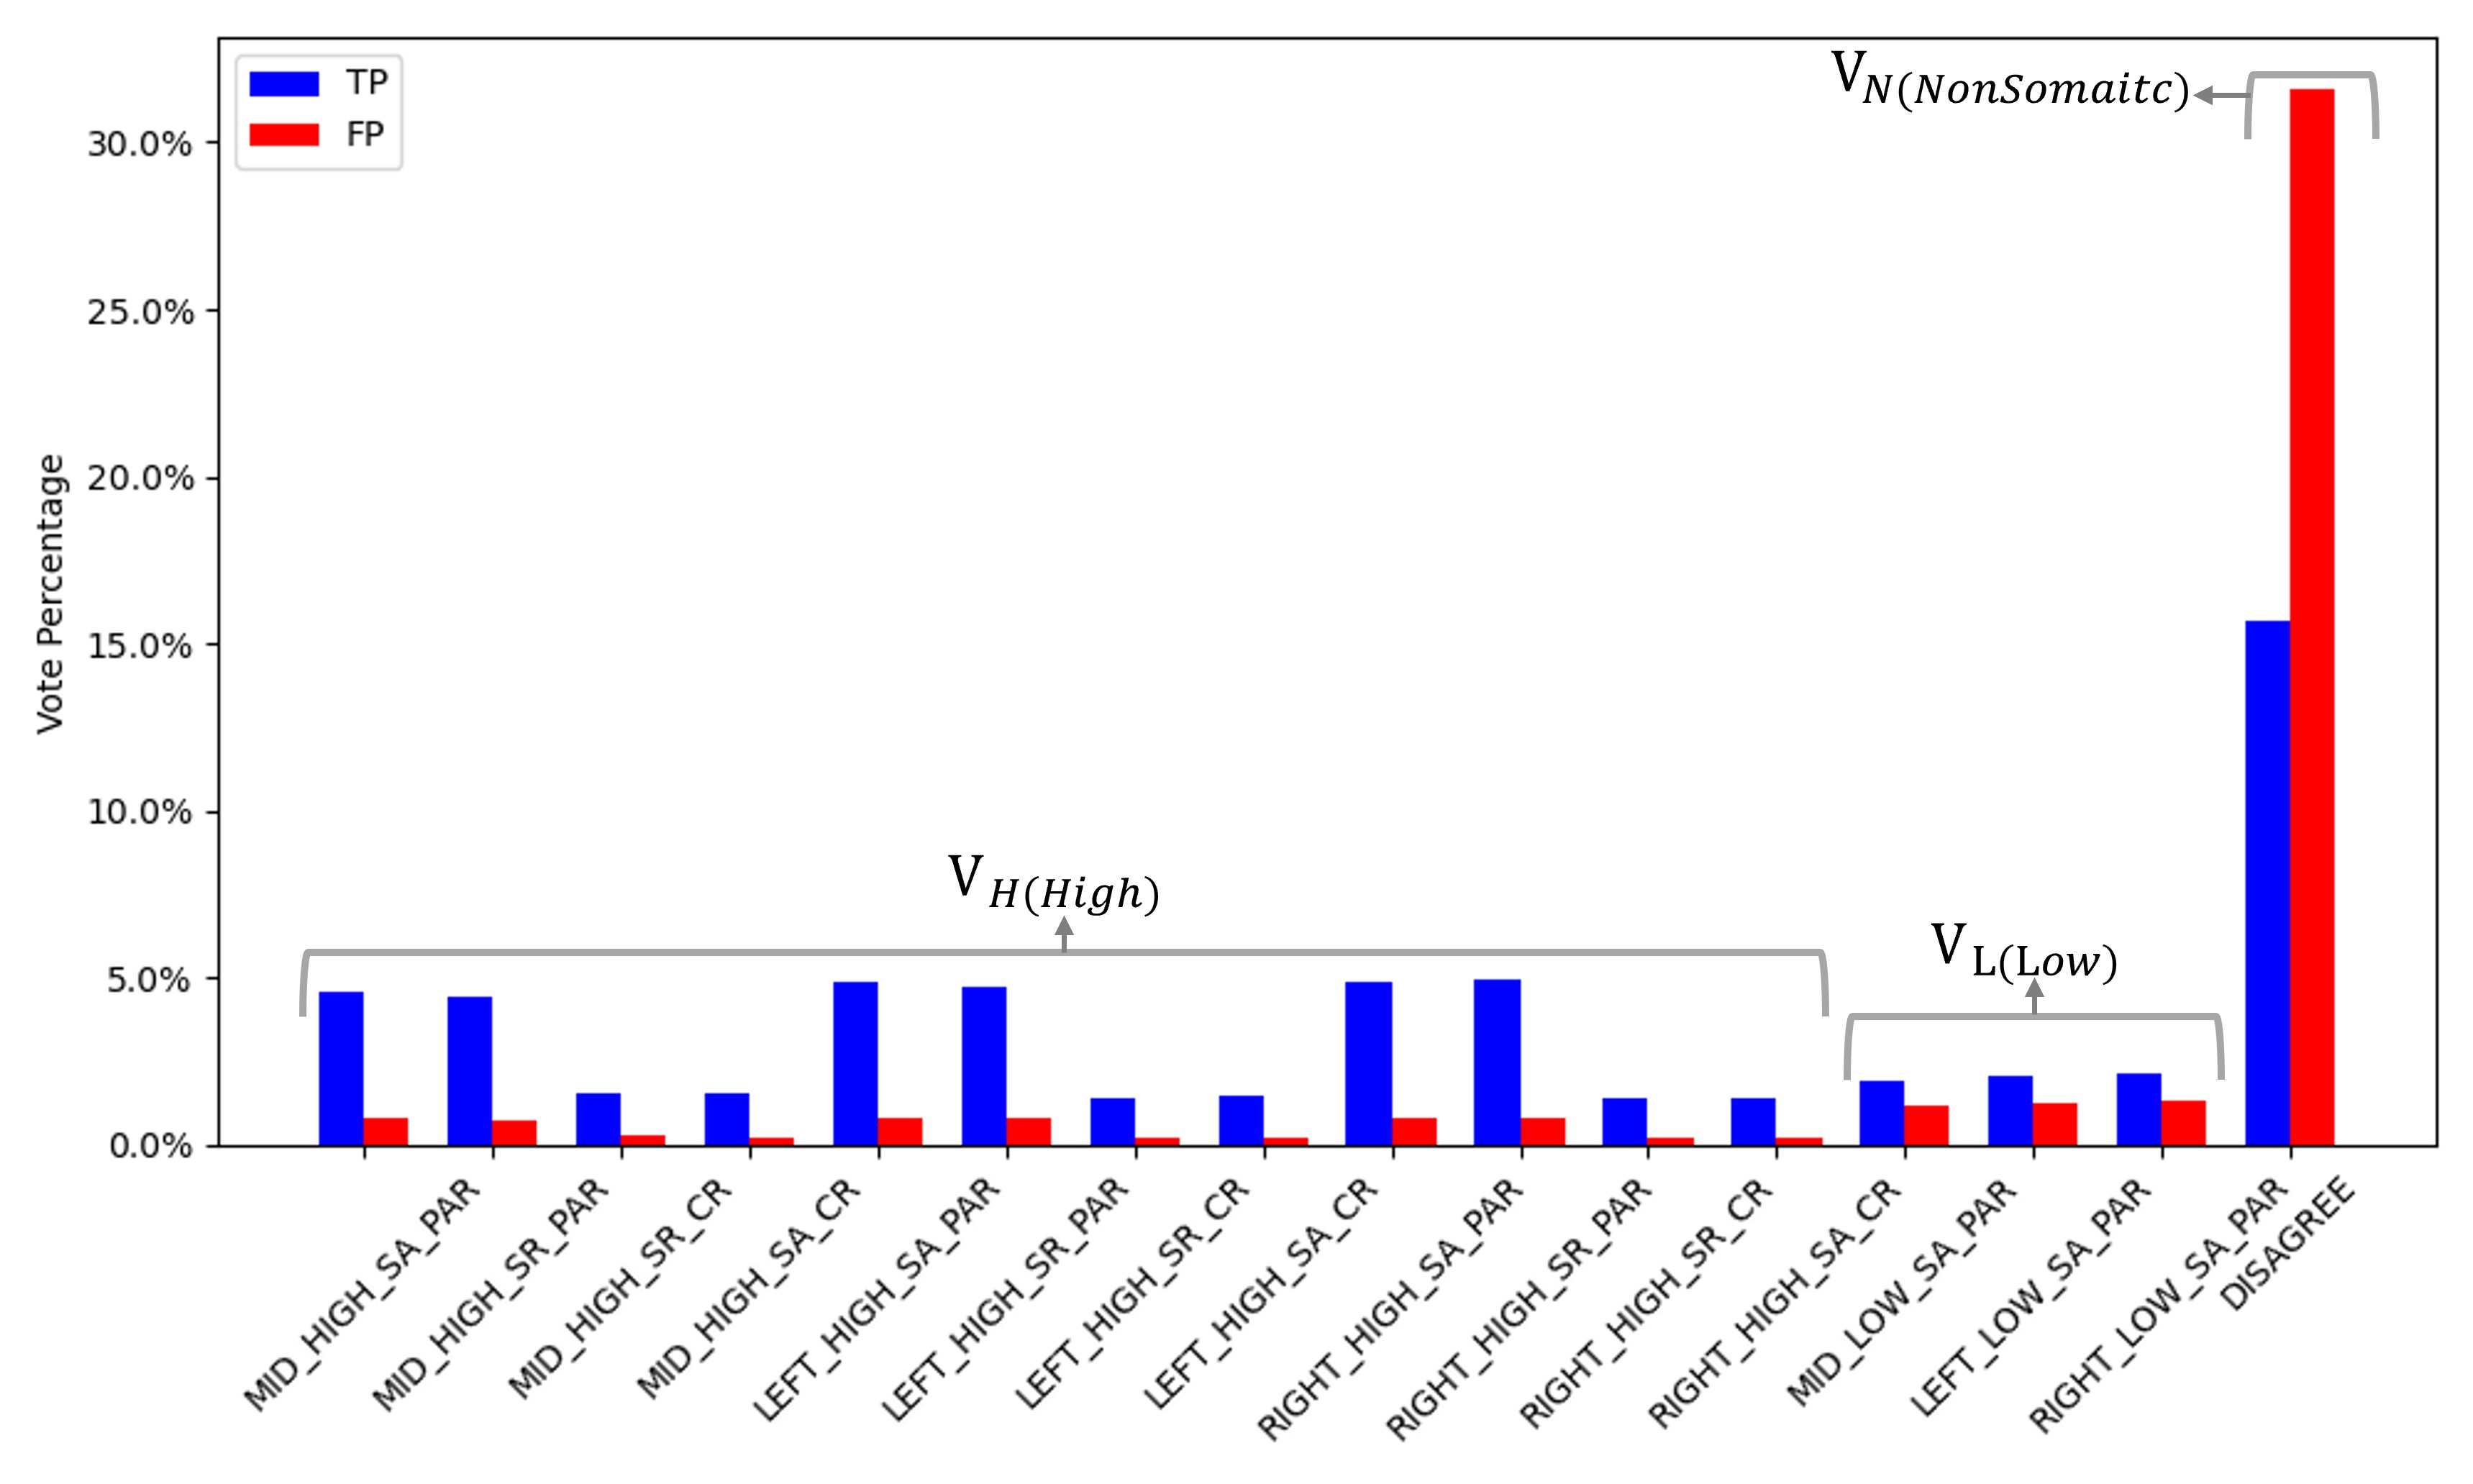
\includegraphics[keepaspectratio]{page_38_cropped.jpg}}
  \caption[Evidence pattern comparison]{Comparison of true positive (TP, blue) and false positive (FP, red) variant calls across predefined evidence patterns. The patterns are grouped into three categories: high-confidence (\(V_H\)), low-confidence (\(V_L\)), and non-somatic (\(V_N\)). \(V_H\) patterns are strongly enriched for TPs with minimal FP contribution, \(V_L\) patterns occur less frequently but remain reliable indicators of true variants, and the \(V_N\) group comprises the single category labeled DISAGREE on the horizontal axis, which contributes substantially to both TPs and FPs and is therefore ambiguous and unreliable. These distributions provide the rationale for adopting a filtering strategy that prioritizes variants supported by \(V_H\) and \(V_L\) patterns.}\label{fig:app-page-38-cropped-jpg}
\end{figure}

\begin{figure}
  \centering
  \pandocbounded{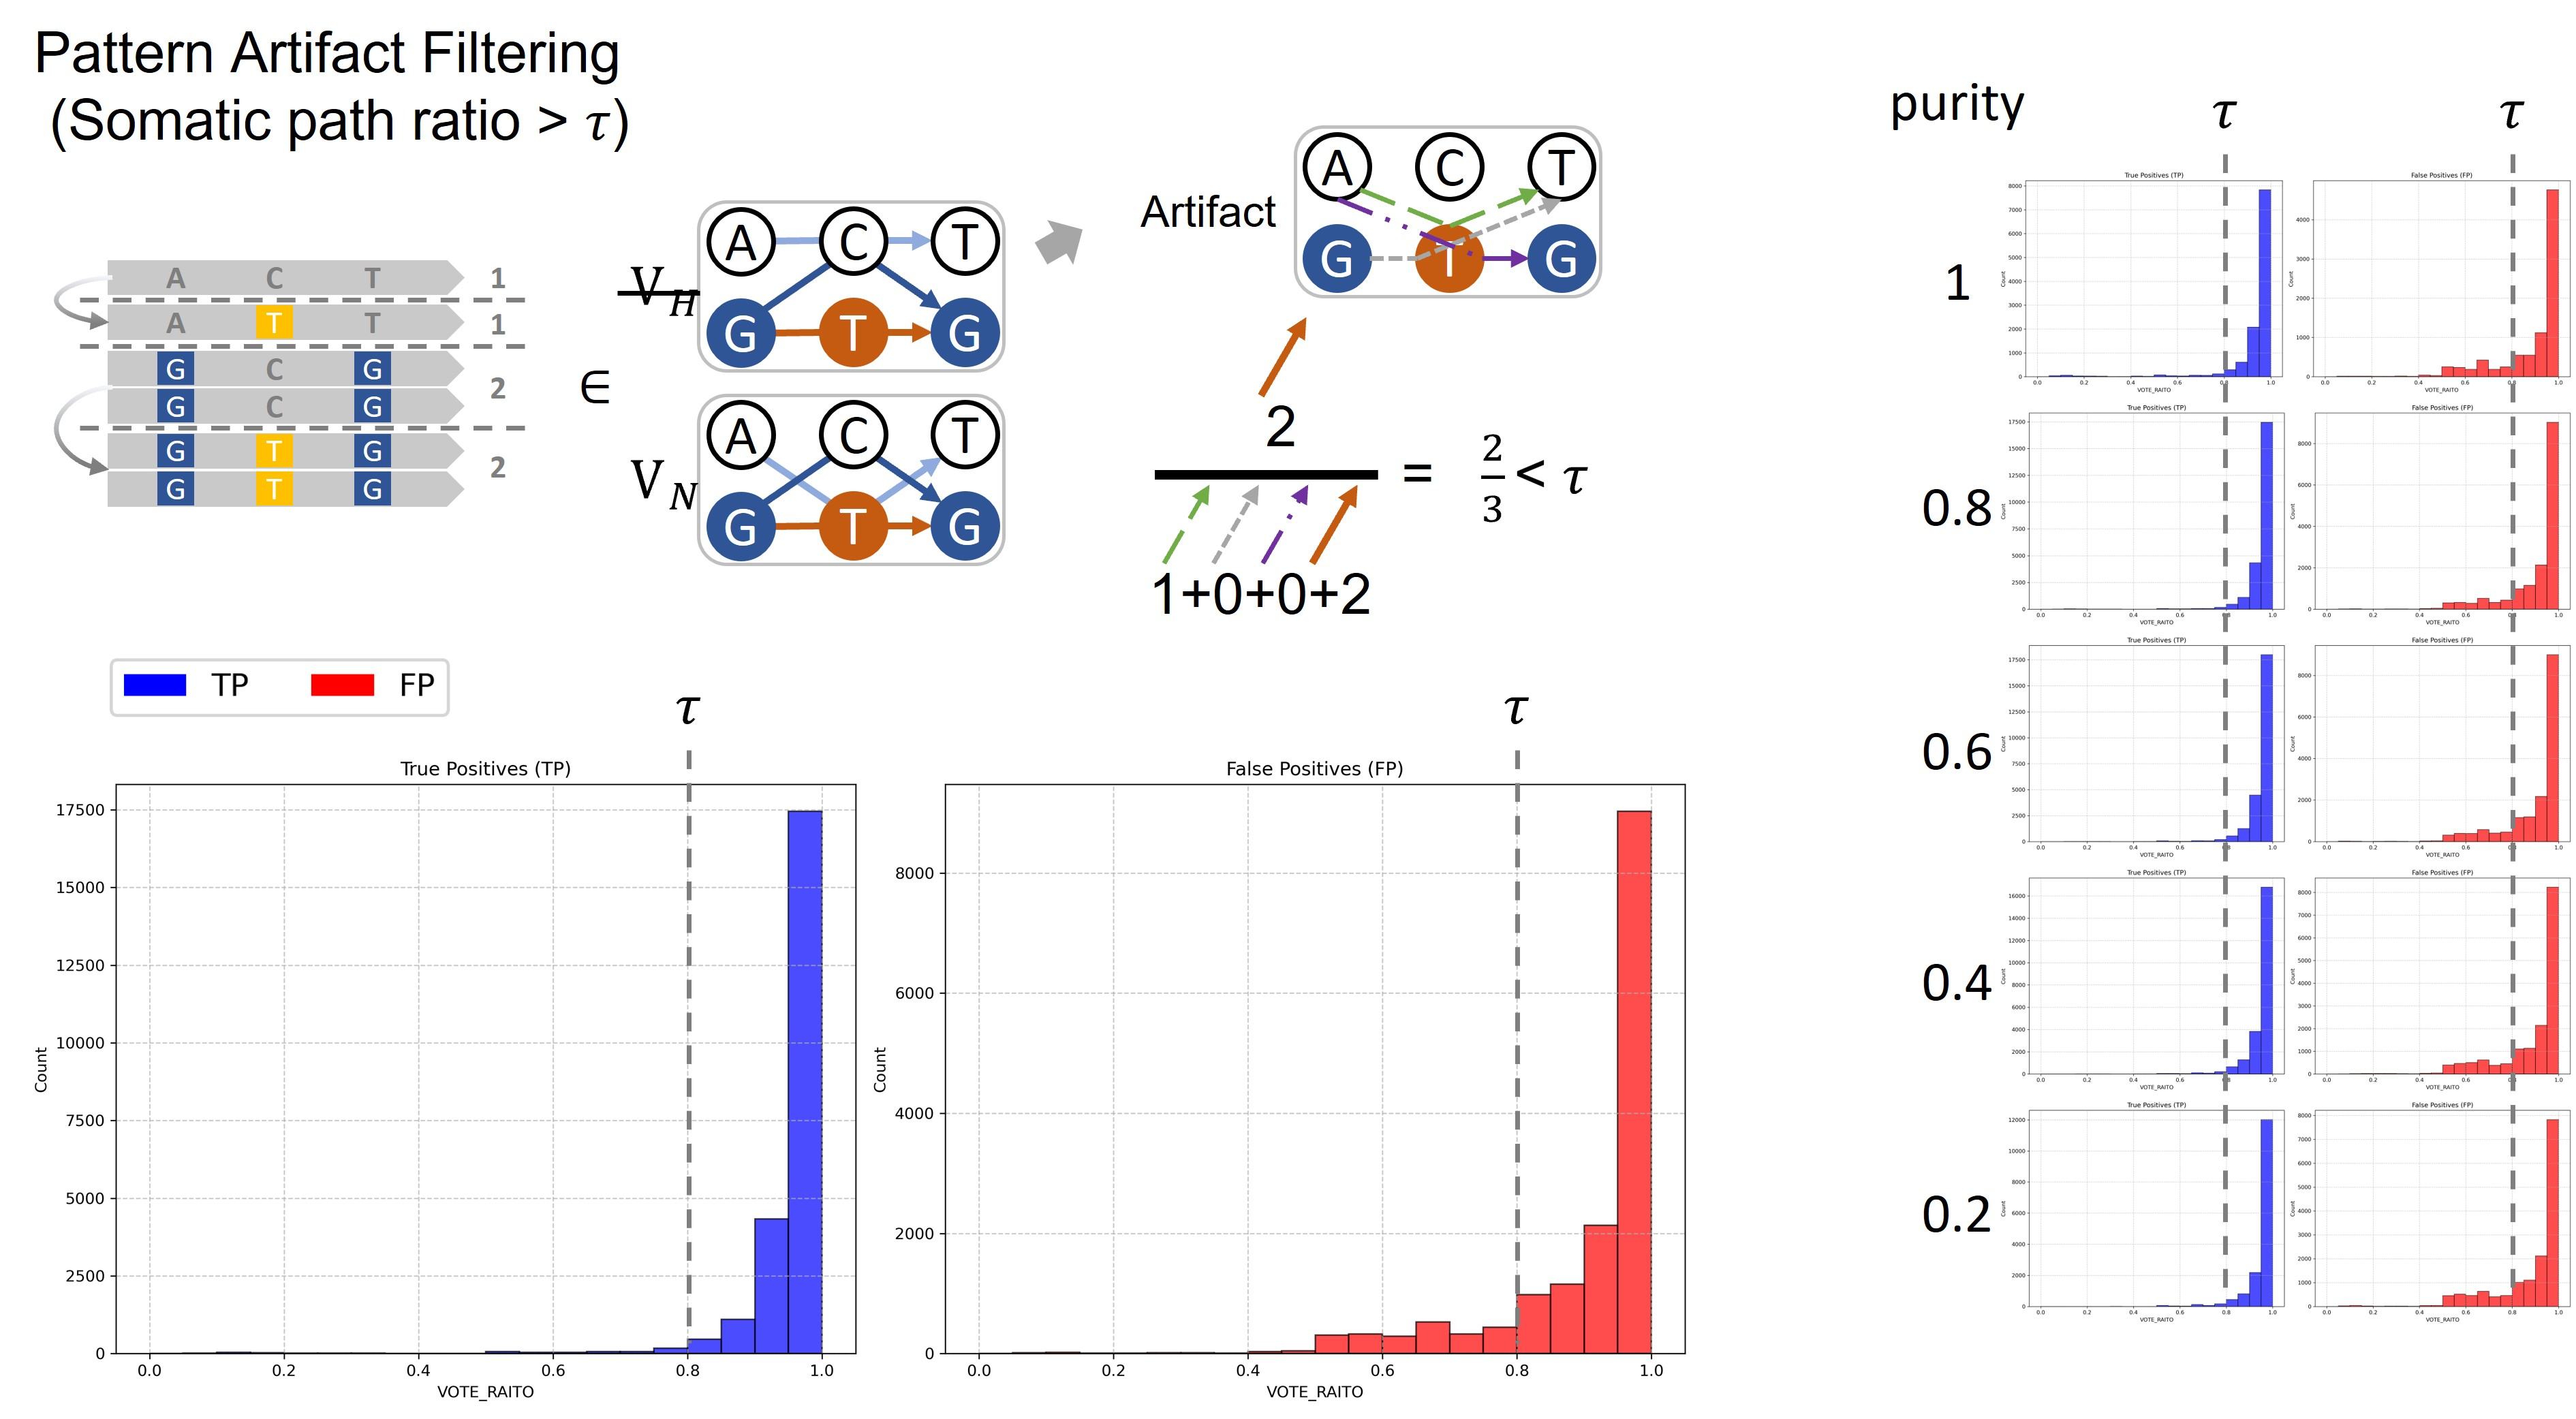
\includegraphics[keepaspectratio]{page_39_cropped.jpg}}
  \caption[High-confidence somatic-path support]{Distribution of the mean high-confidence somatic-path proportion, \(S_H\), used during site-level evidence aggregation. True positive candidates (TP, blue) are enriched near 1.0, whereas false positive candidates (FP, red) have lower and more dispersed values. The separation across tumor DNA fractions from 1.0 to 0.2 supports the retained threshold \(S_H>\tau\), where \(\tau=0.8\), for candidates with at least one regression-accepted \(V_H\) triplet.}\label{fig:app-page-39-cropped-jpg}
\end{figure}

\begin{figure}
  \centering
  \pandocbounded{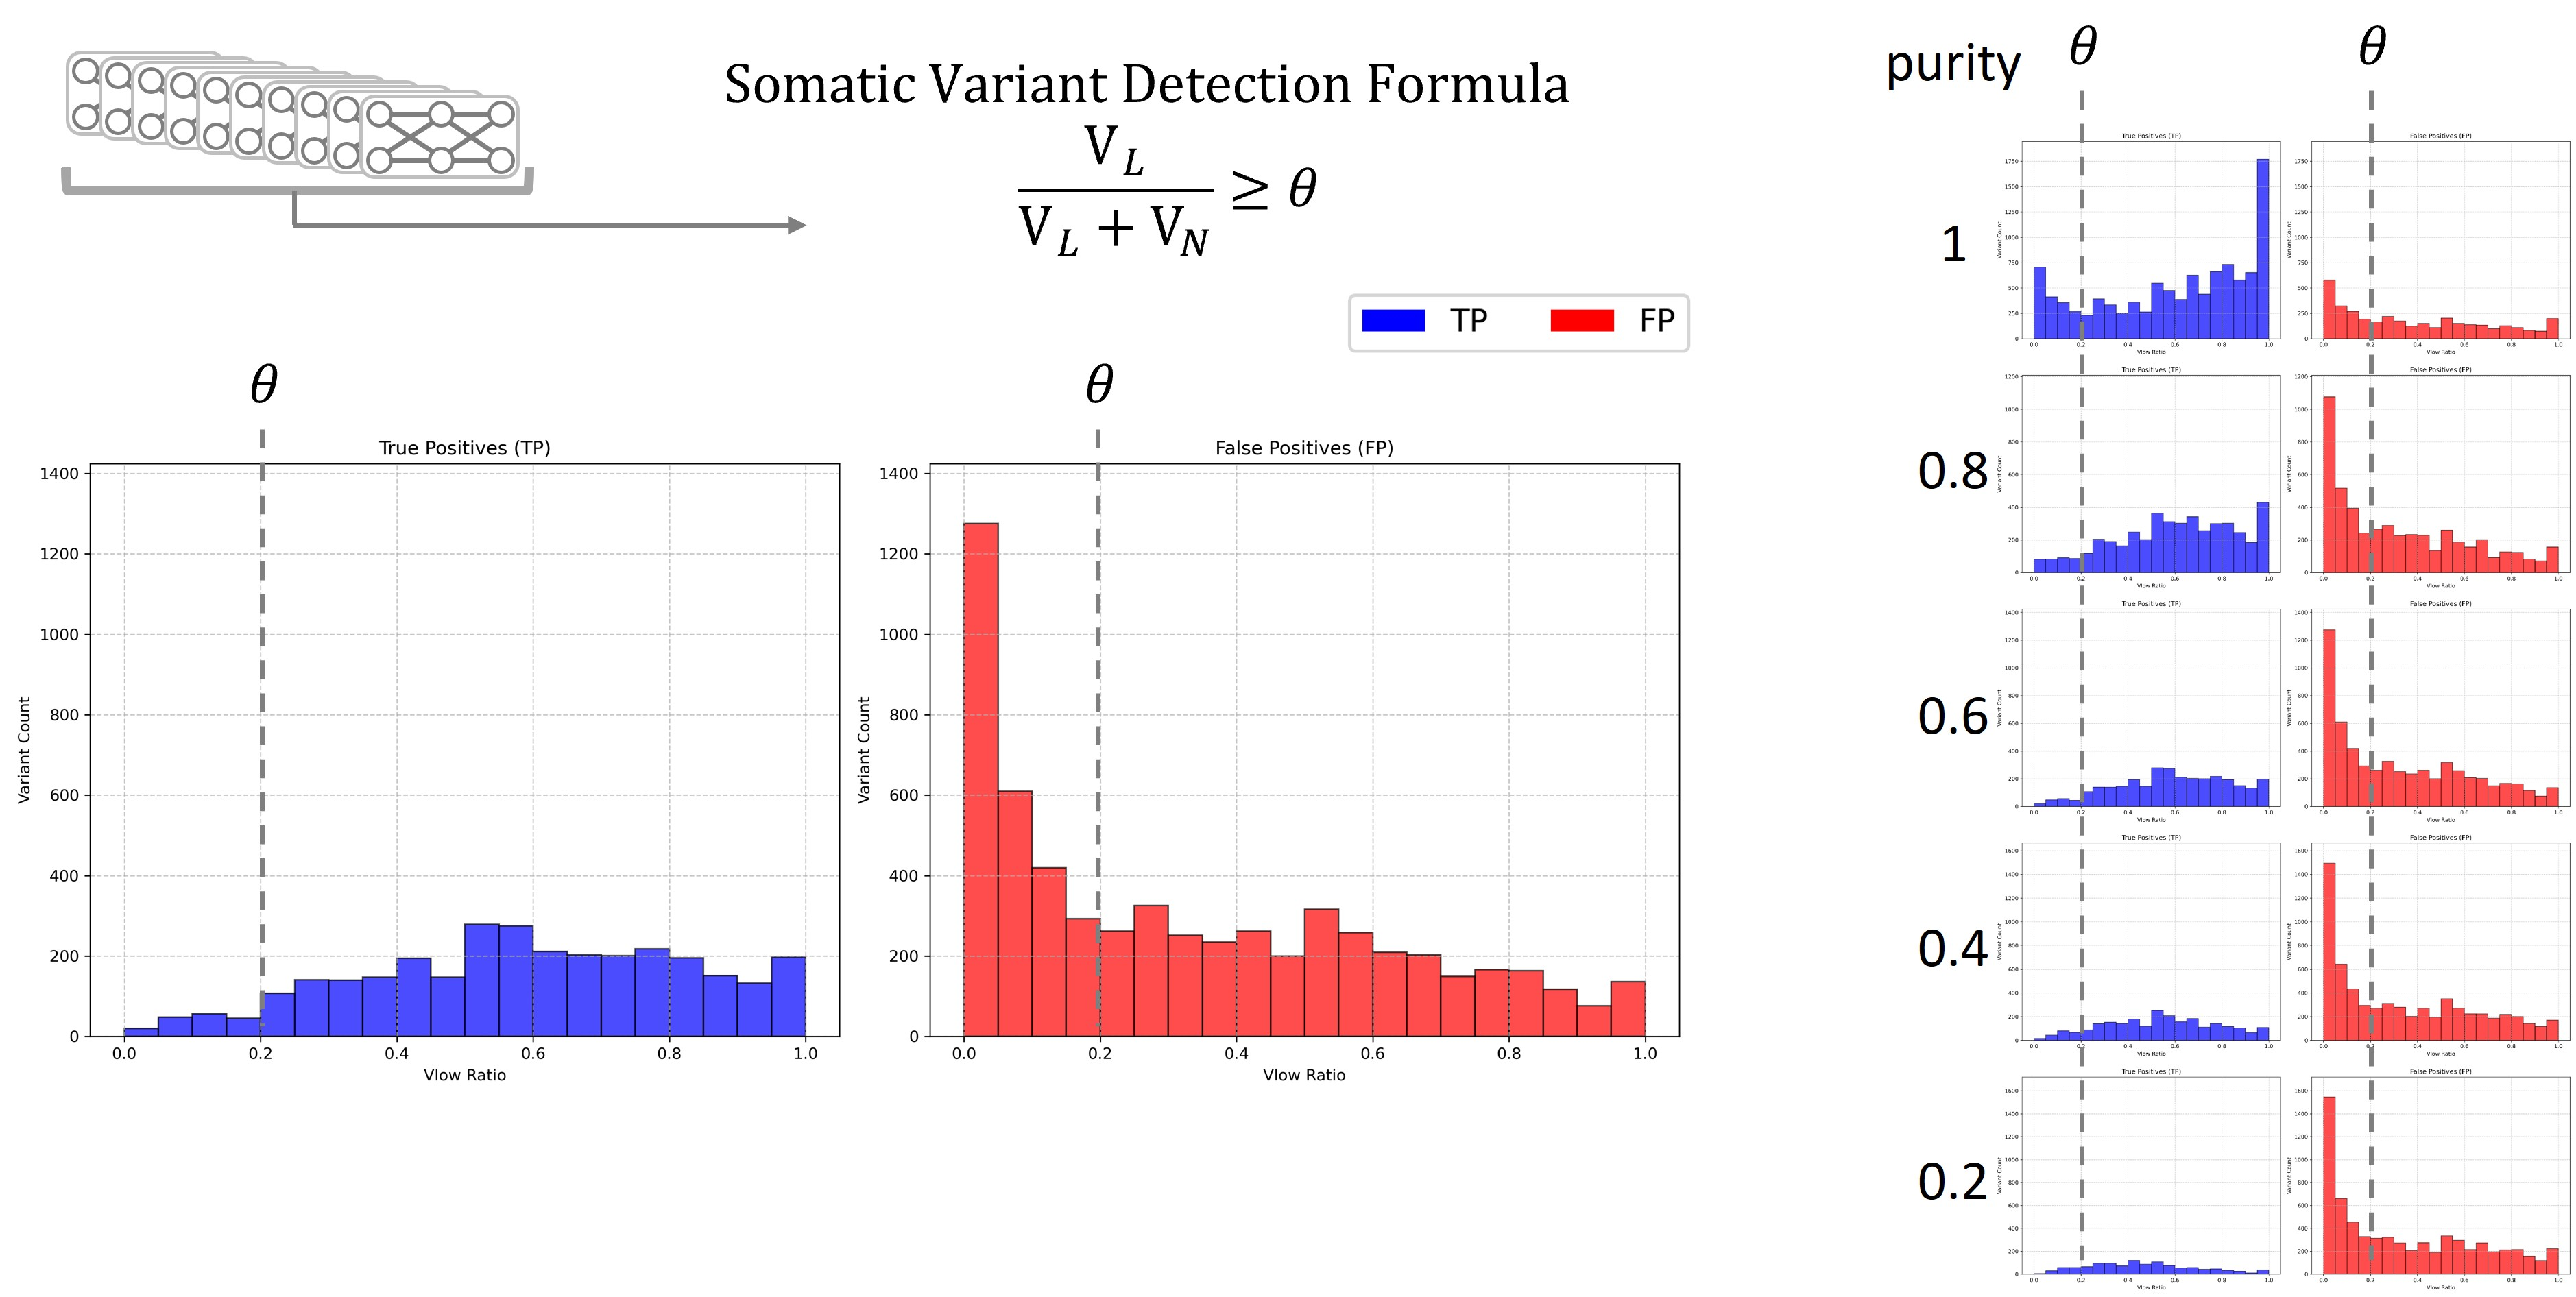
\includegraphics[keepaspectratio]{page_40_cropped.jpg}}
  \caption[Low-confidence evidence fraction]{Distribution of the site-level low-confidence evidence fraction, \(L/(L+N)\), for validated true positive (TP, blue) and false positive (FP, red) candidates. False positive candidates are concentrated near zero, whereas true positive candidates extend toward higher values. The distributions across tumor DNA fractions from 1.0 to 0.2 support the retained threshold \(L/(L+N)\geq\theta\), where \(\theta=0.2\), when no high-confidence route is satisfied.}\label{fig:app-page-40-cropped-jpg}
\end{figure}

\begin{figure}
  \centering
  \pandocbounded{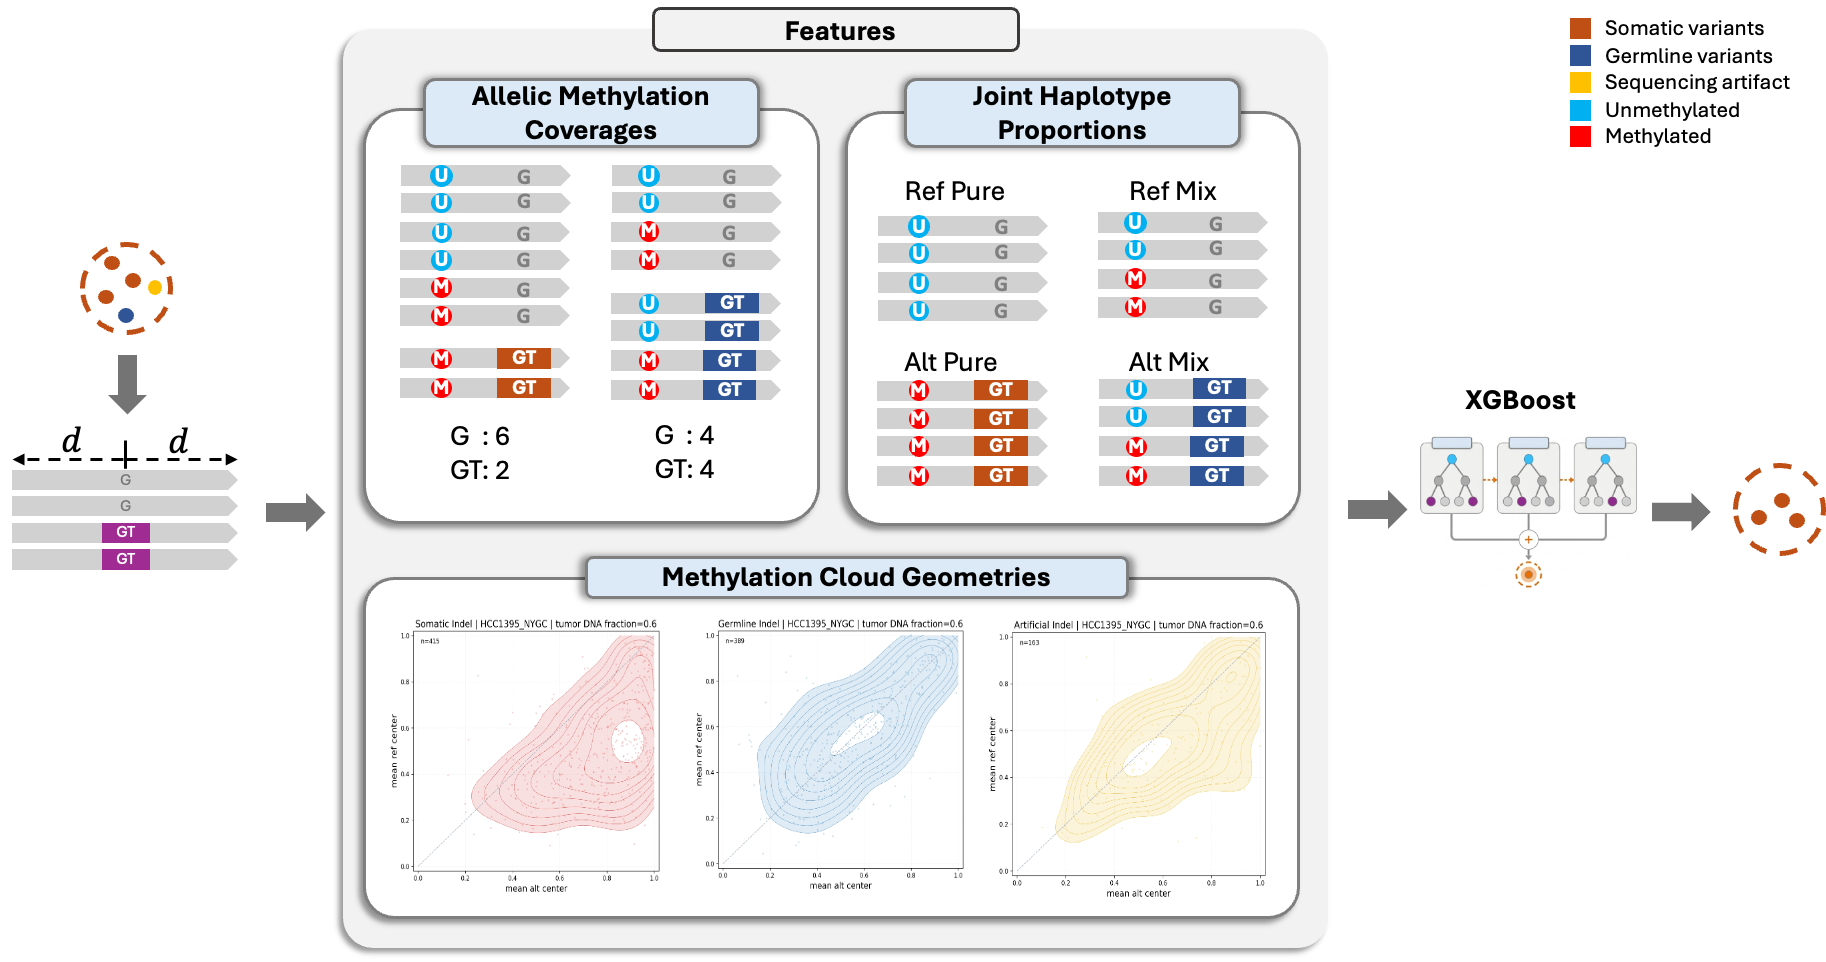
\includegraphics[width=\textwidth,keepaspectratio]{methylation_overview.png}}
  \caption[Methylation-aware recalibration overview]{Overview of methylation-aware recalibration of somatic variant candidates. When the input alignments carry 5-methylcytosine (5mC) tags, reads spanning each candidate are partitioned by the allele they carry at the candidate locus (reference, ``G'', or alternate, e.g.\ ``GT''), and the CpG sites within a symmetric window of $\pm d$ base pairs are analyzed at single-read resolution (methylated, red ``M'', and unmethylated, cyan ``U''). Ten features are computed across three complementary views: allelic methylation coverage (per-site methylated-read counts on each allele), joint haplotype methylation proportions (per-site classification of each allele as methylation-pure or methylation-mixed), and methylation-cloud geometry (per-site allele methylation ratios and the geometry of their centroid, with kernel-density clouds shown for somatic, germline and artifact indels in HCC1395\_NYGC at 0.6 tumor DNA fraction). A gradient-boosted decision-tree classifier (XGBoost) uses these features to label each candidate as a somatic variant, germline variant or sequencing artifact, retaining only candidates classified as somatic.}\label{fig:met-methylation-overview}
\end{figure}

\begin{figure}
  \centering
  \pandocbounded{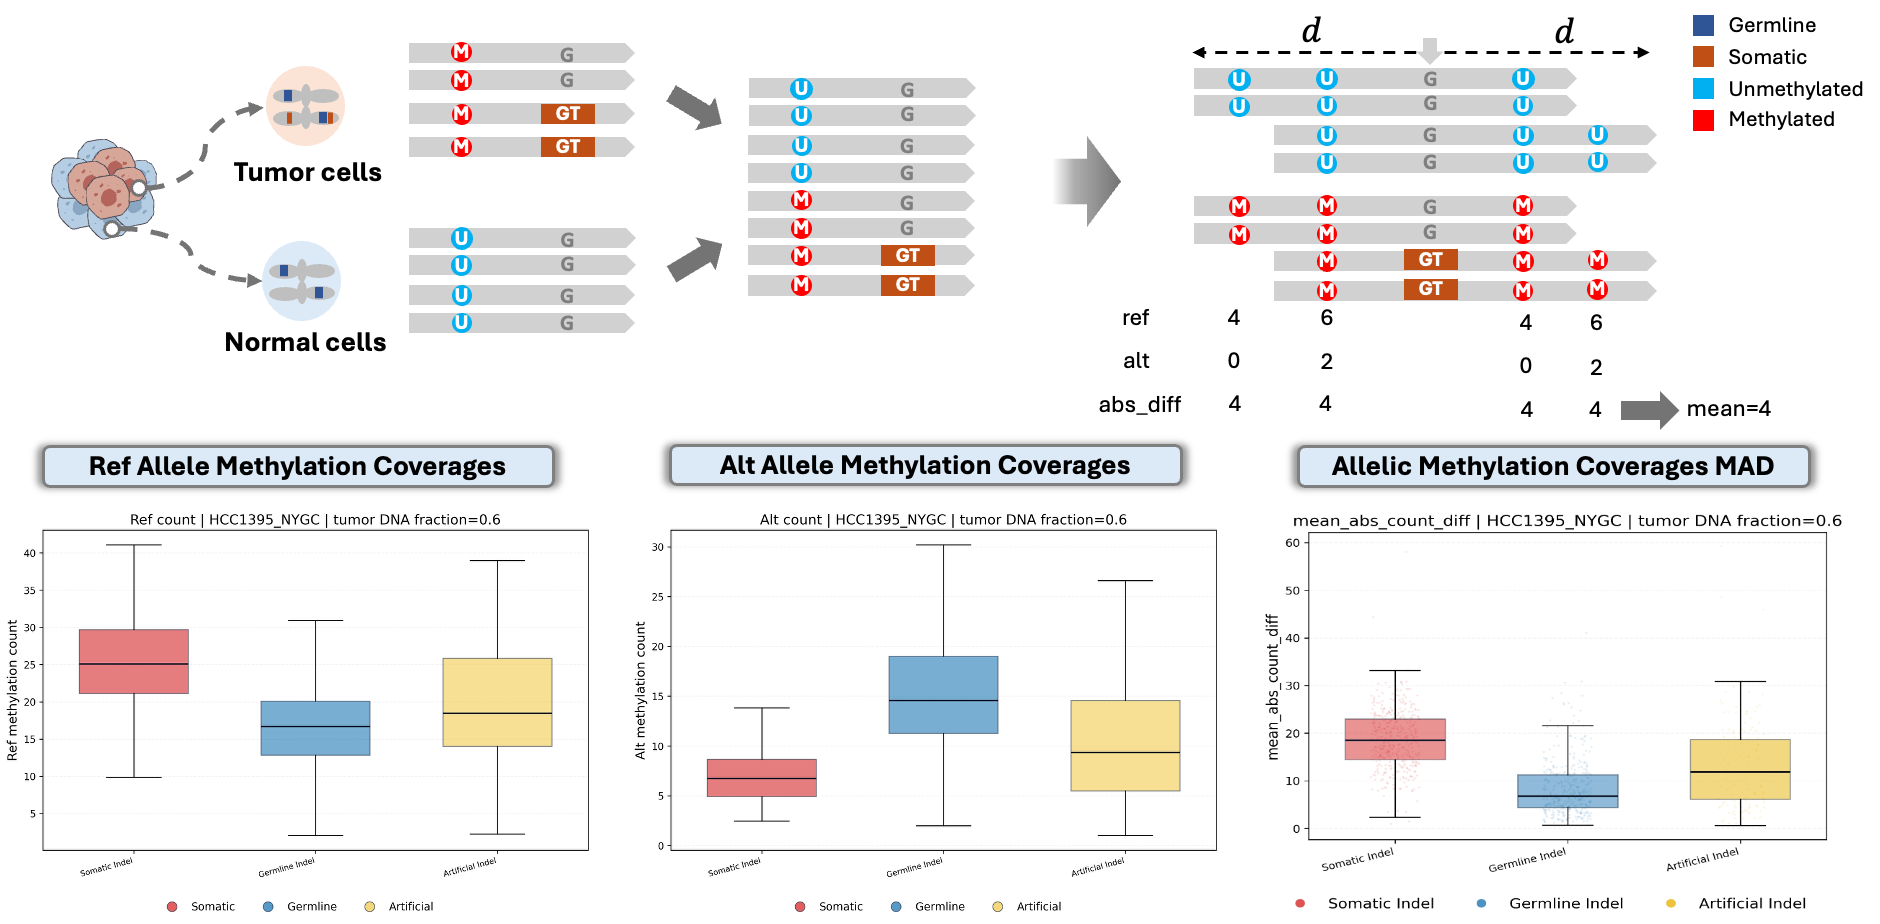
\includegraphics[width=\textwidth,keepaspectratio]{methylation_allelic_coverage.png}}
  \caption[Allelic methylation coverage features]{Allelic methylation coverage features. Reads spanning a candidate are split by the allele they carry (reference, ``G'', or alternate, e.g.\ ``GT''), and at each CpG site within the flanking window the number of methylated reads is counted separately for the two alleles (methylated, red ``M'', and unmethylated, cyan ``U''). The per-site reference and alternate methylated-read counts and their absolute difference are averaged over the window to give the mean reference count, the mean alternate count and the mean absolute count difference (MAD). Because the somatic alternate allele is confined to the uniformly methylated tumor fraction, whereas the reference allele mixes tumor- and normal-derived reads, somatic indels exhibit the largest allelic count difference. Box plots (HCC1395\_NYGC at 0.6 tumor DNA fraction) contrast somatic, germline and artifact indels for each feature.}\label{fig:met-methylation-allelic}
\end{figure}

\begin{figure}
  \centering
  \pandocbounded{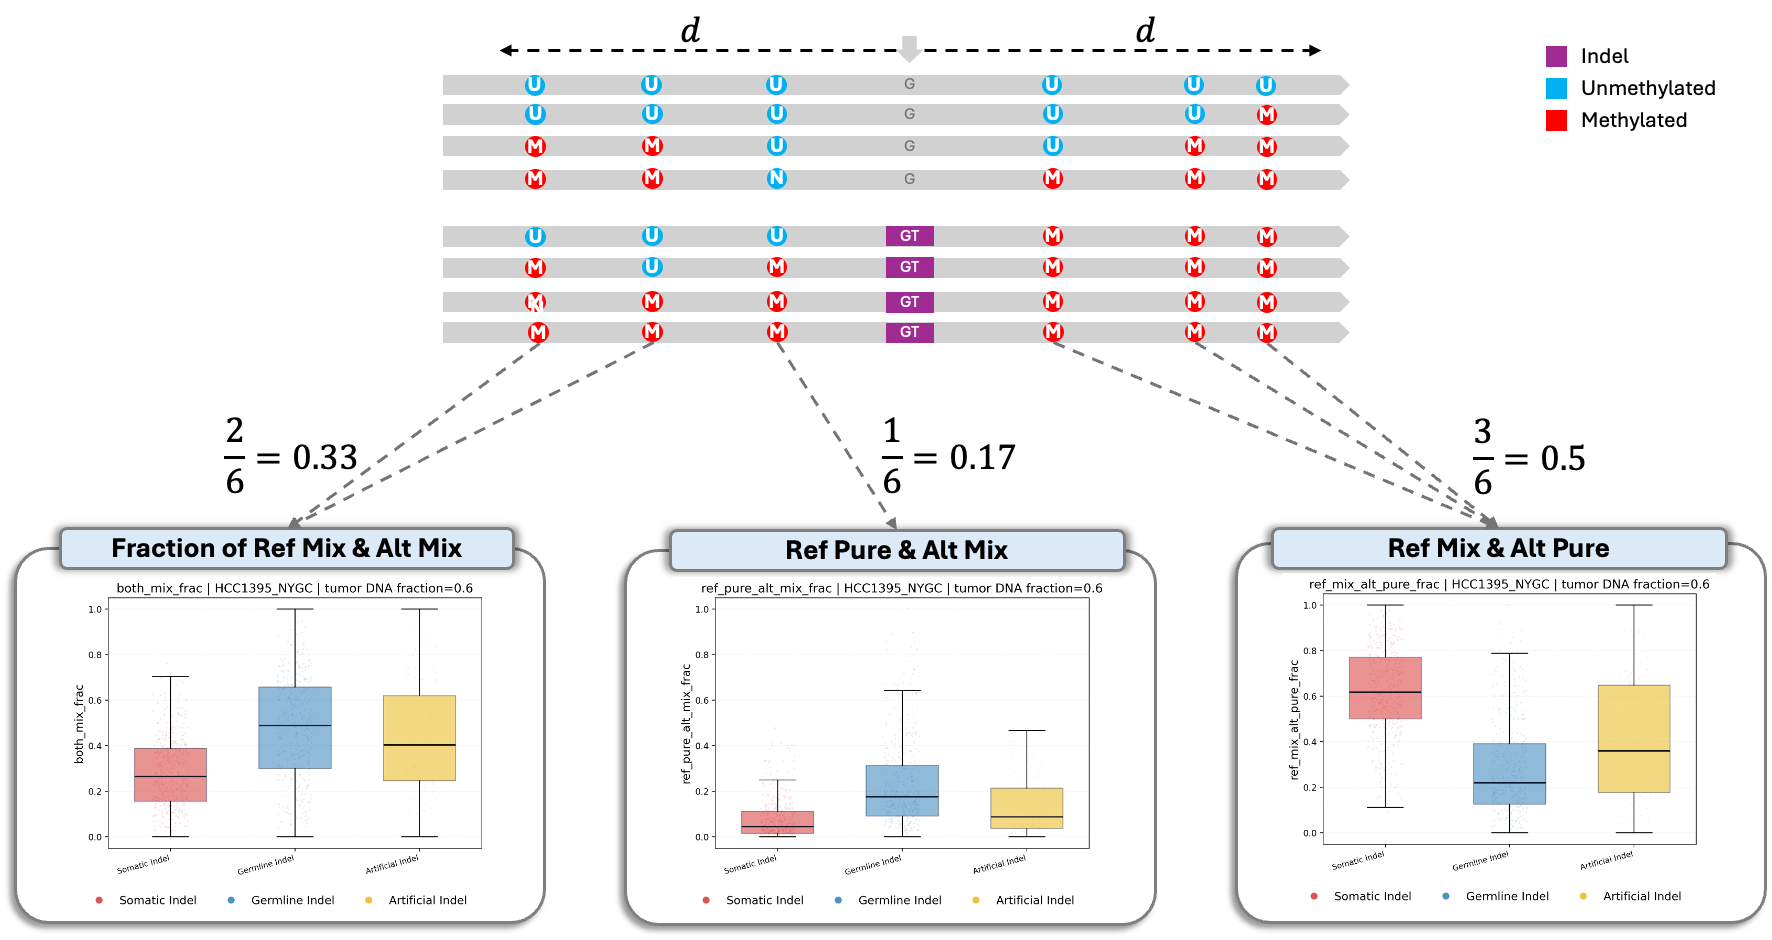
\includegraphics[width=\textwidth,keepaspectratio]{methylation_joint_haplotype.png}}
  \caption[Joint haplotype methylation proportion features]{Joint haplotype methylation proportion features. At each CpG site within the flanking window, the reads of each allele are labeled ``pure'' when they share a single methylation state (all methylated, red ``M'', or all unmethylated, cyan ``U'') and ``mixed'' when both states are present. Pairing the reference- and alternate-allele labels assigns each site to one of four joint states, and the fraction of covered CpG sites in each state is recorded, and three of the four proportions are retained as features (the fourth is redundant, as they sum to one). In the illustrated window of six covered CpG sites, the reference-mixed/alternate-mixed, reference-pure/alternate-mixed and reference-mixed/alternate-pure fractions are $2/6=0.33$, $1/6=0.17$ and $3/6=0.5$, respectively. The somatic signature of a methylation-pure alternate allele against a methylation-mixed reference allele is captured by an elevated reference-mixed/alternate-pure fraction. Box plots (HCC1395\_NYGC at 0.6 tumor DNA fraction) contrast somatic, germline and artifact indels for each feature.}\label{fig:met-methylation-joint}
\end{figure}

\begin{figure}
  \centering
  \pandocbounded{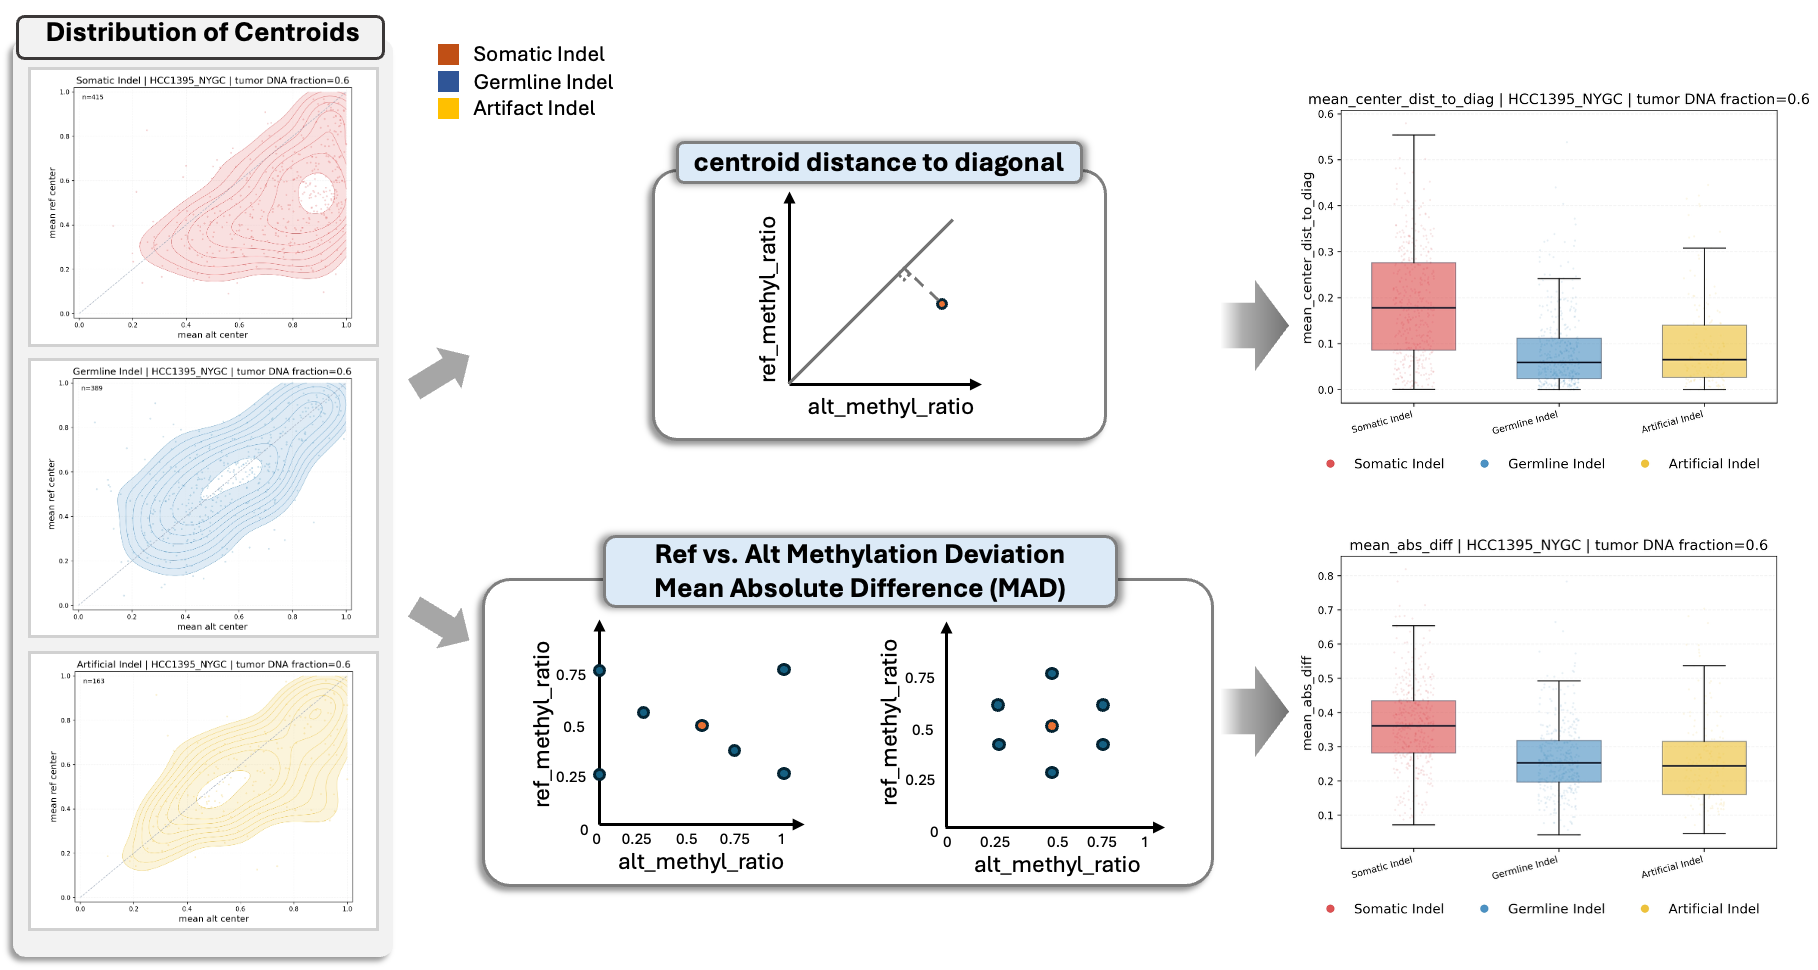
\includegraphics[width=\textwidth,keepaspectratio]{methylation_cloud_geometry.png}}
  \caption[Methylation-cloud geometry features]{Methylation-cloud geometry features. At each CpG site within the flanking window, an allele methylation ratio is computed for the reference and alternate alleles, and the per-site (alternate ratio, reference ratio) points form a cloud whose centroid (mean alternate ratio, mean reference ratio) is retained as two features, and the kernel-density distributions of these centroids differ between somatic, germline and artifact indels (left). Two further features summarize the cloud geometry: the perpendicular distance of the centroid from the diagonal $y=x$, which quantifies the overall imbalance between reference- and alternate-allele methylation, and the mean absolute per-site difference between the reference and alternate ratios (MAD). Balanced methylation places the centroid near the diagonal, whereas the allele-specific methylation of a somatic variant displaces it. Box plots (HCC1395\_NYGC at 0.6 tumor DNA fraction) show that somatic indels have the largest centroid-to-diagonal distance and ratio MAD.}\label{fig:met-methylation-cloud}
\end{figure}

\begin{figure}
  \centering
  \pandocbounded{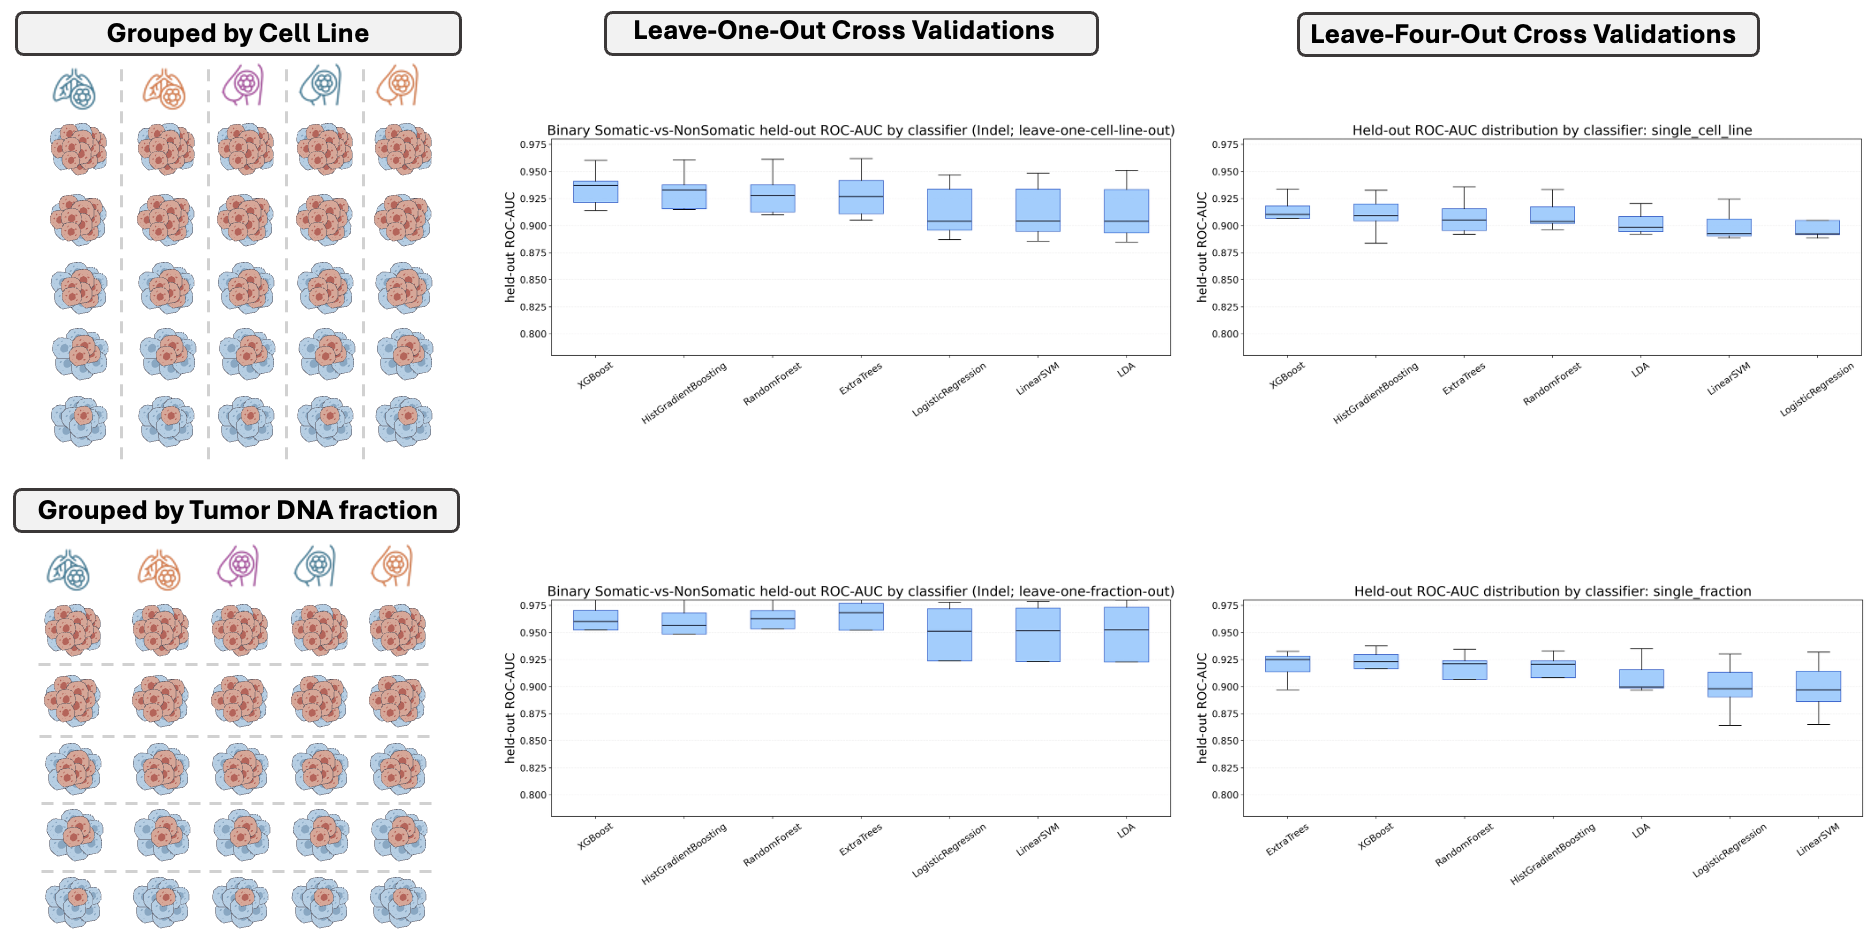
\includegraphics[width=\textwidth,keepaspectratio]{methylation_classifier_selection.png}}
  \caption[Classifier selection for methylation-aware recalibration]{Selection of the classifier for methylation-aware recalibration. Seven candidate classifiers were compared by held-out ROC-AUC on the binary somatic-versus-non-somatic indel task under two cross-validation schemes, each applied both across cell lines and across tumor DNA fractions. Left, leave-one-out cross-validation, in which the model is trained on all groups but one and evaluated on the held-out group. Right, leave-four-out cross-validation, in which it is trained on a single group and evaluated on the remaining four. The four tree-ensemble methods (XGBoost, histogram-based gradient boosting, random forests and extremely randomized trees) outperform the three linear methods (logistic regression, a linear support-vector machine and linear discriminant analysis), and XGBoost is consistently the top or tied-top performer. Its held-out ROC-AUC remains high even under the more stringent leave-four-out setting, supporting both the choice of XGBoost and the single-sample training strategy. The box plots convey the quantitative results, and the cell-line and tumor-fraction icons are schematic.}\label{fig:met-classifier-selection}
\end{figure}

\begin{figure}
  \centering
  \pandocbounded{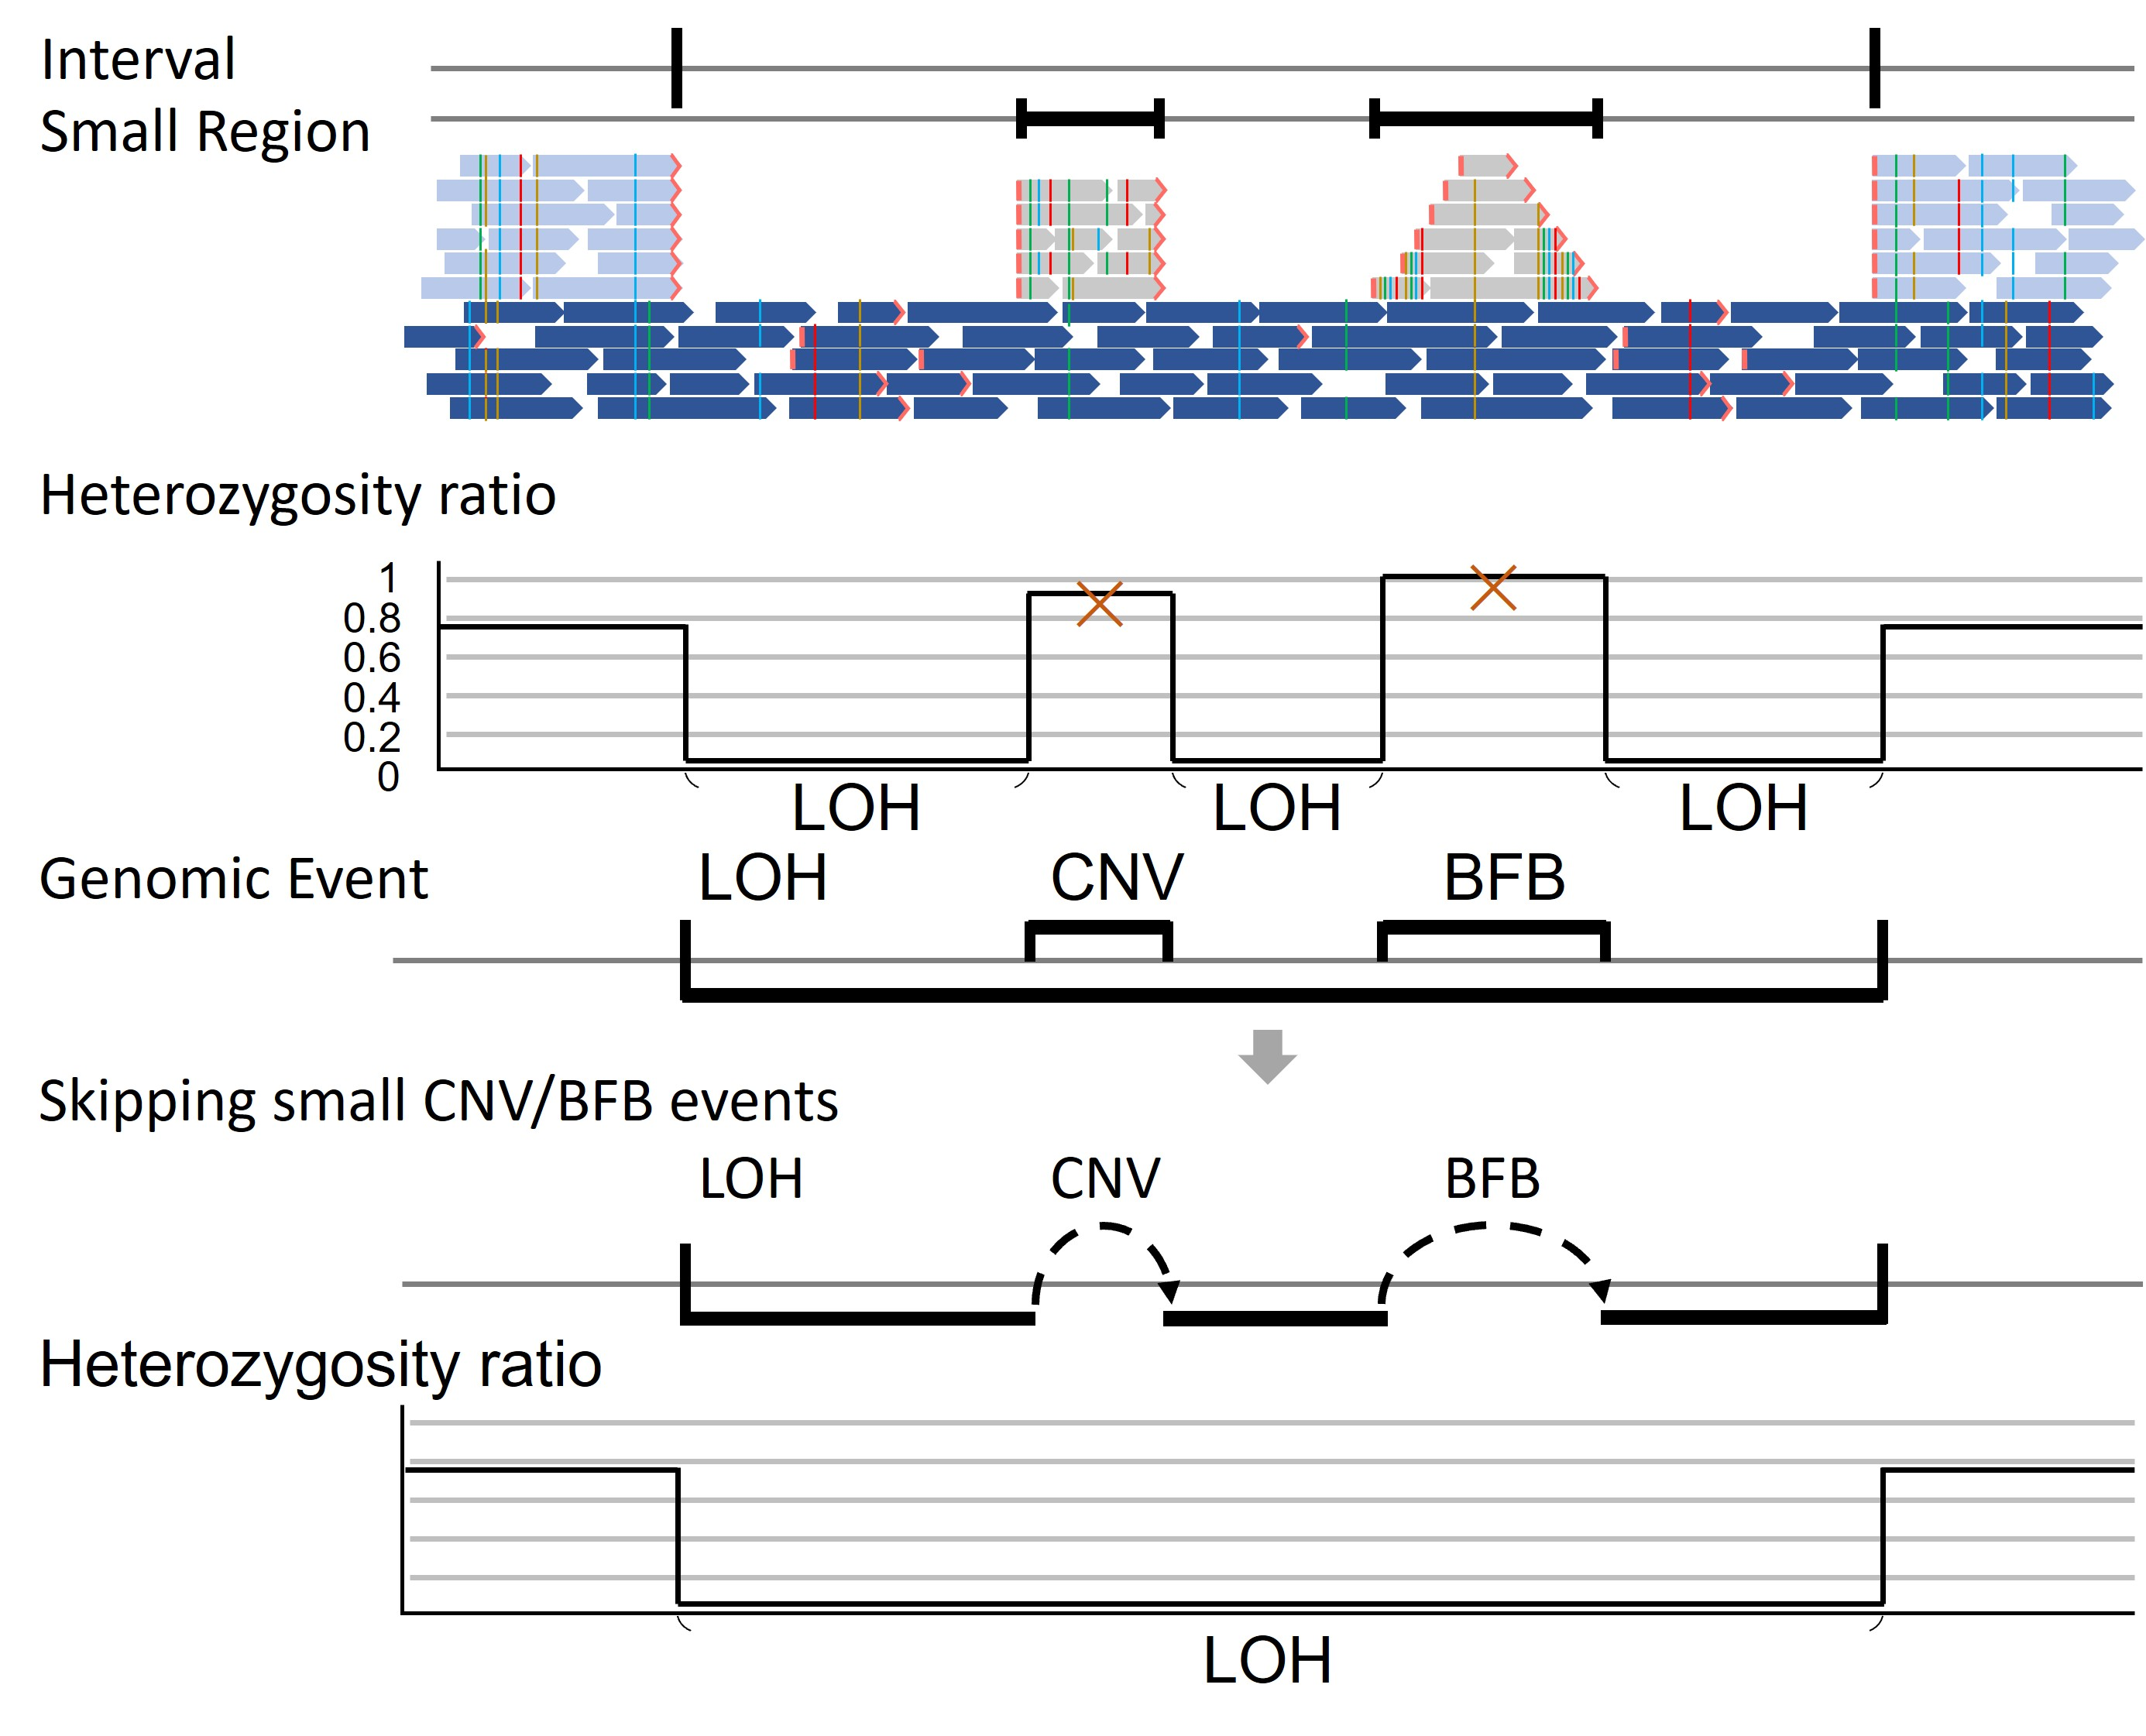
\includegraphics[width=0.8\textwidth, keepaspectratio]{page_17_cropped.jpg}}
  \caption[Chromosome-scale LOH detection]{Chromosome-scale LOH detection after exclusion of short CNV/BFB-associated intervals. Candidate LOH boundaries define the region evaluated. Small CNV or BFB events embedded within a broader LOH tract can locally increase heterozygosity and split an initial LOH call. Omitting variants within these short intervals before calculating the regional heterozygosity ratio allows the flanking heterozygosity-depleted segments to be classified as one continuous arm-level LOH event.}\label{fig:met-page-17-cropped-jpg}
\end{figure}

\begin{figure}
  \centering
  \pandocbounded{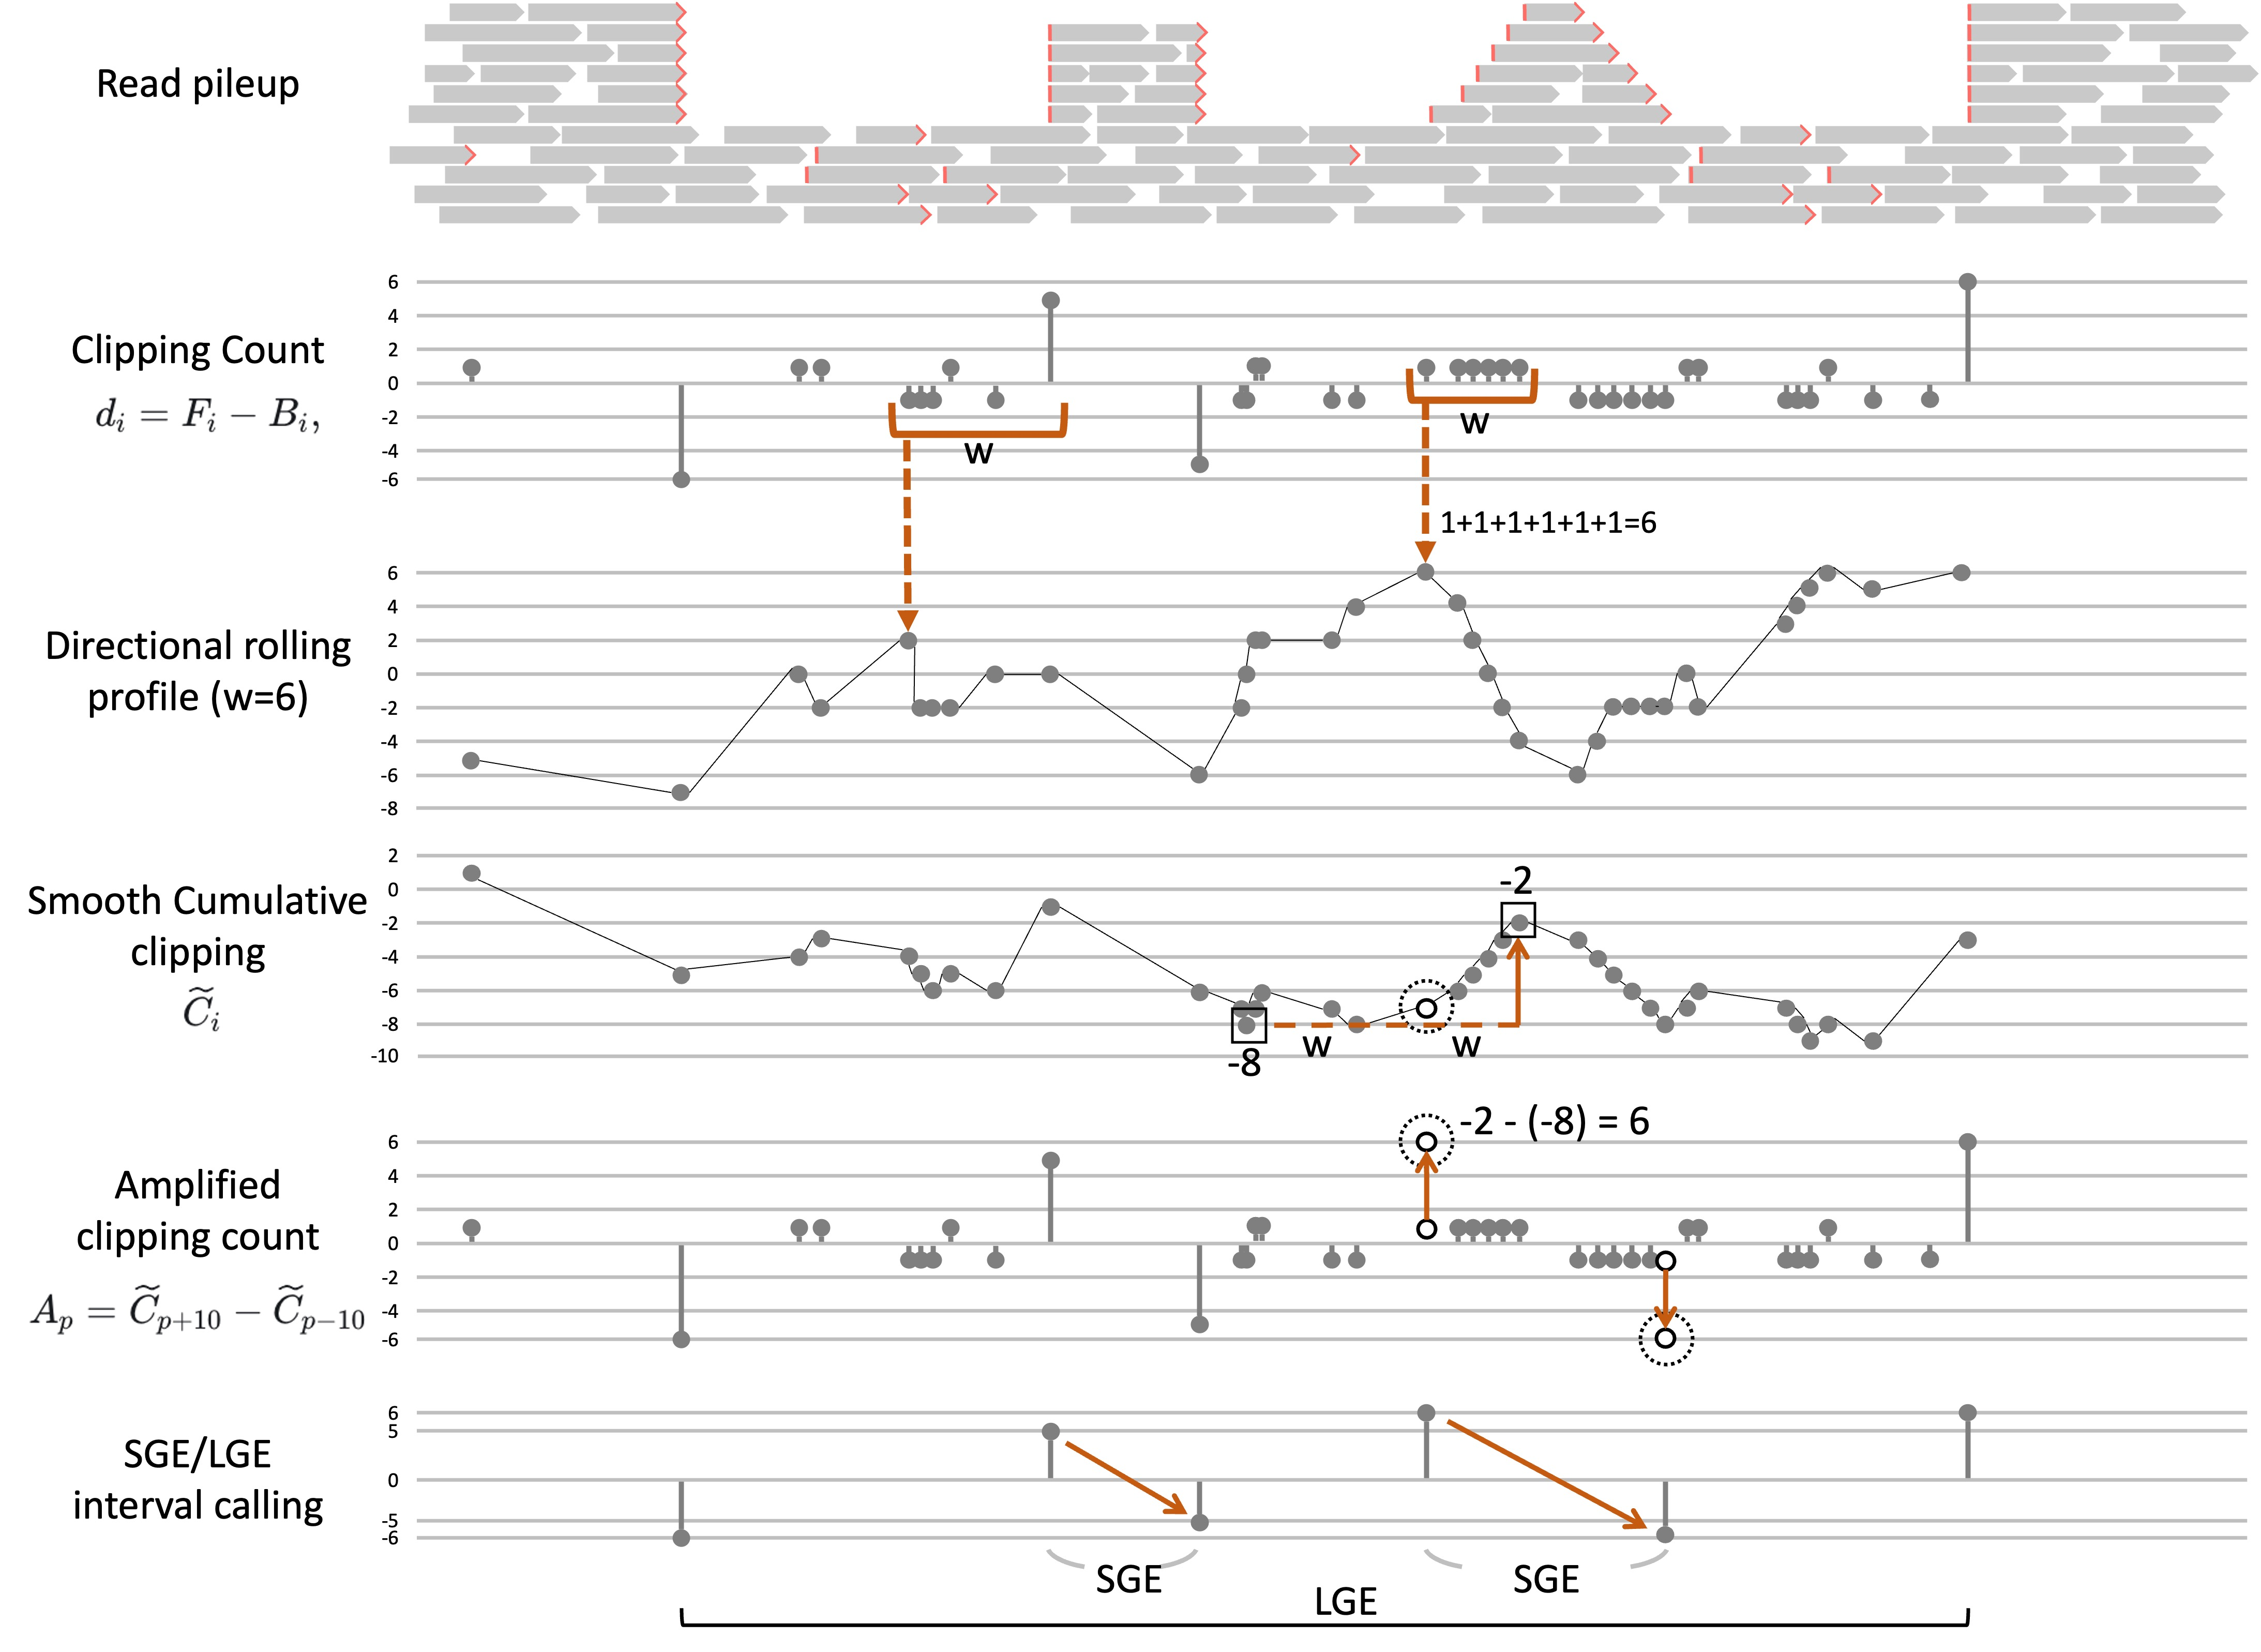
\includegraphics[keepaspectratio]{page_14_cropped.jpg}}
  \caption[Breakpoint detection and small CNV/BFB interval pairing from read clipping]{Breakpoint detection and small CNV/BFB interval pairing from read clipping. Soft- and hard-clipping operations longer than five bases are counted at the left and right alignment ends as $F_i$ and $B_i$, respectively, and their difference defines the signed directional signal, $d_i=F_i-B_i$. Strong localized signals are retained without smoothing, whereas directional rolling profiles consolidate dispersed lower-amplitude support. For each resulting candidate at position $p$, support is estimated from the change in the smoothed cumulative clipping signal across the candidate, $A_p=\widetilde{C}_{p+10}-\widetilde{C}_{p-10}$, whose sign preserves clipping orientation. Nearby signals of opposite orientation are paired to delimit short intervals associated with local CNV or BFB events, labeled small genomic events (SGE), whereas unpaired signals are retained as candidate boundaries of broader LOH regions, labeled large genomic events (LGE). The schematic uses a six-position rolling window for clarity, and full definitions and fixed implementation parameters are provided in Supplementary Methods (Section~\ref{supp:directional-clipping}) and Supplementary Table~\ref{tab:loh-clipping-parameters}. SGE and LGE are operational labels and do not assign a molecular event subtype.
  }\label{fig:met-page-14-cropped-jpg}
\end{figure}

\begin{figure}
  \centering
  \pandocbounded{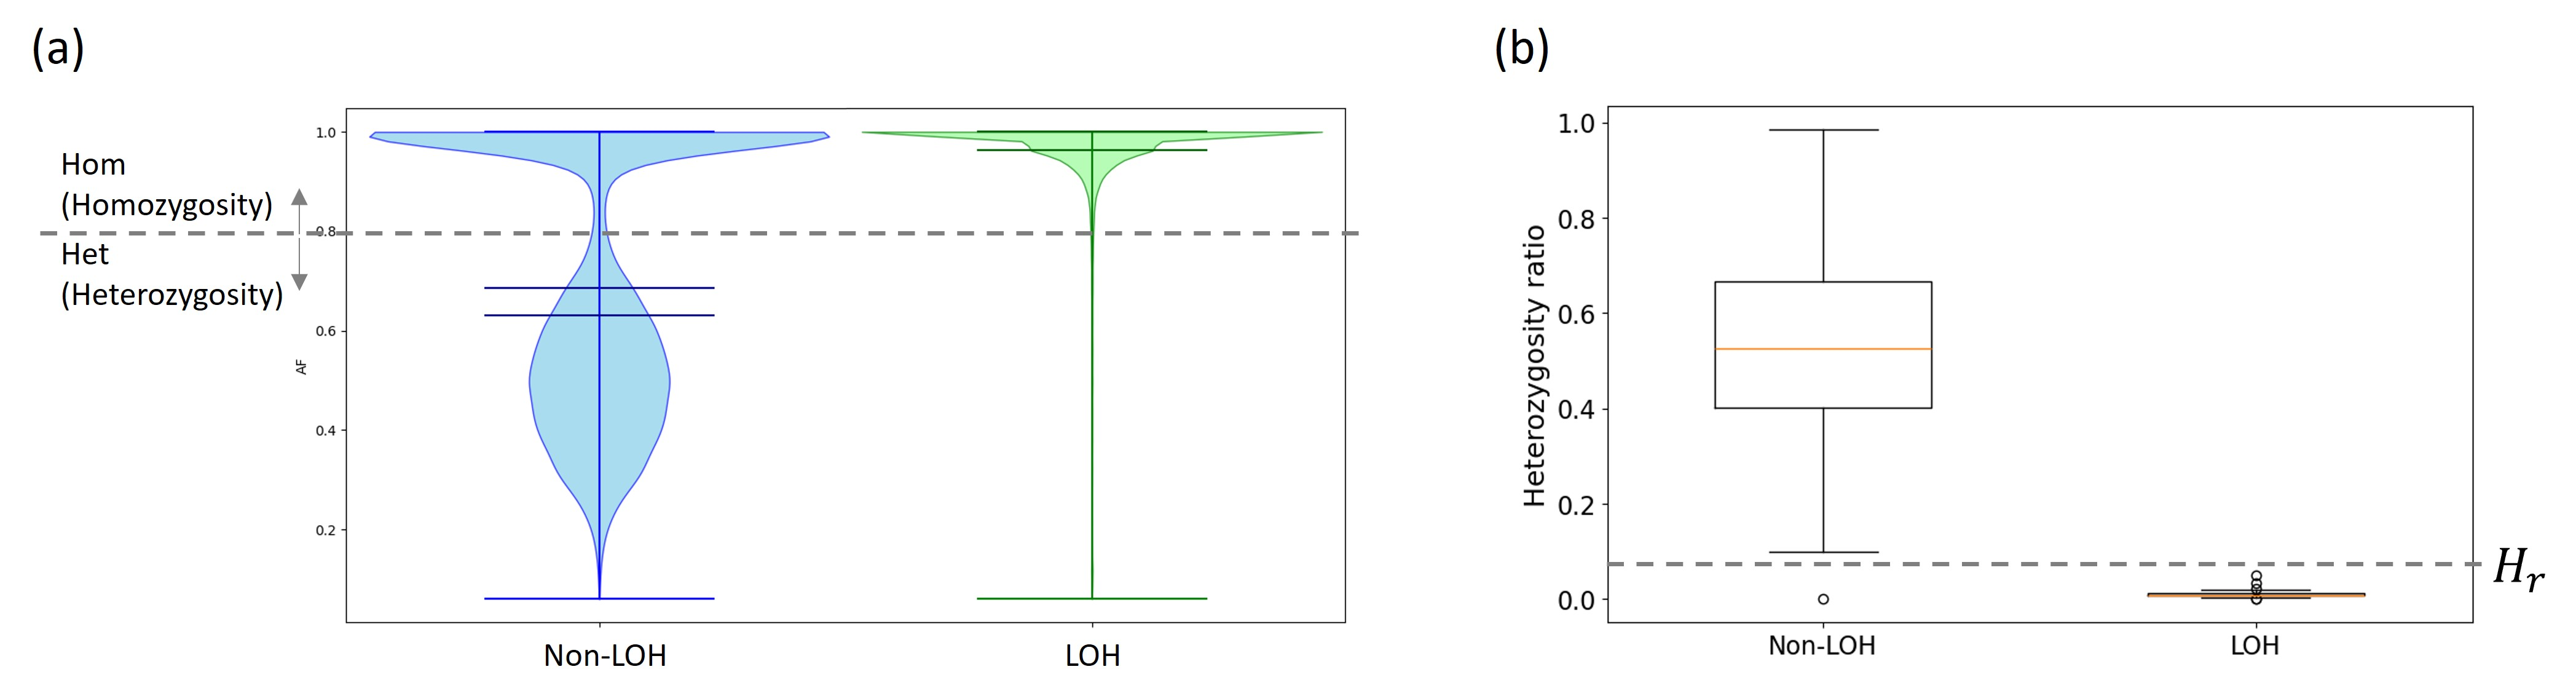
\includegraphics[keepaspectratio]{page_37_cropped.jpg}}
  \caption[Empirical calibration of LOH classification thresholds]{Empirical calibration of LOH classification thresholds using the HCC1395 LOH and non-LOH reference intervals published by SEQC2. (a) Variant allele frequency (VAF) distributions for variants in non-LOH (blue) and LOH (green) regions. The depletion of the heterozygous VAF peak in LOH regions supports classifying variants with VAF $\geq0.8$ as homozygous. (b) Distributions of the regional heterozygosity ratio, $R_{\mathrm{het}}=N_{\mathrm{het}}/(N_{\mathrm{het}}+N_{\mathrm{hom}})$, after exclusion of short CNV/BFB-associated intervals. The separation between non-LOH and LOH regions supports classifying regions with $R_{\mathrm{het}}<0.09$ as LOH. Both thresholds were fixed and applied unchanged across all sequencing datasets.}\label{fig:app-page-37-cropped-jpg}
\end{figure}

% The former distributed-clipping and breakpoint-interval figures were merged
% into the directional-clipping figure above. Their source blocks are retained
% below as comments.
% \begin{figure}
%   \centering
%   \pandocbounded{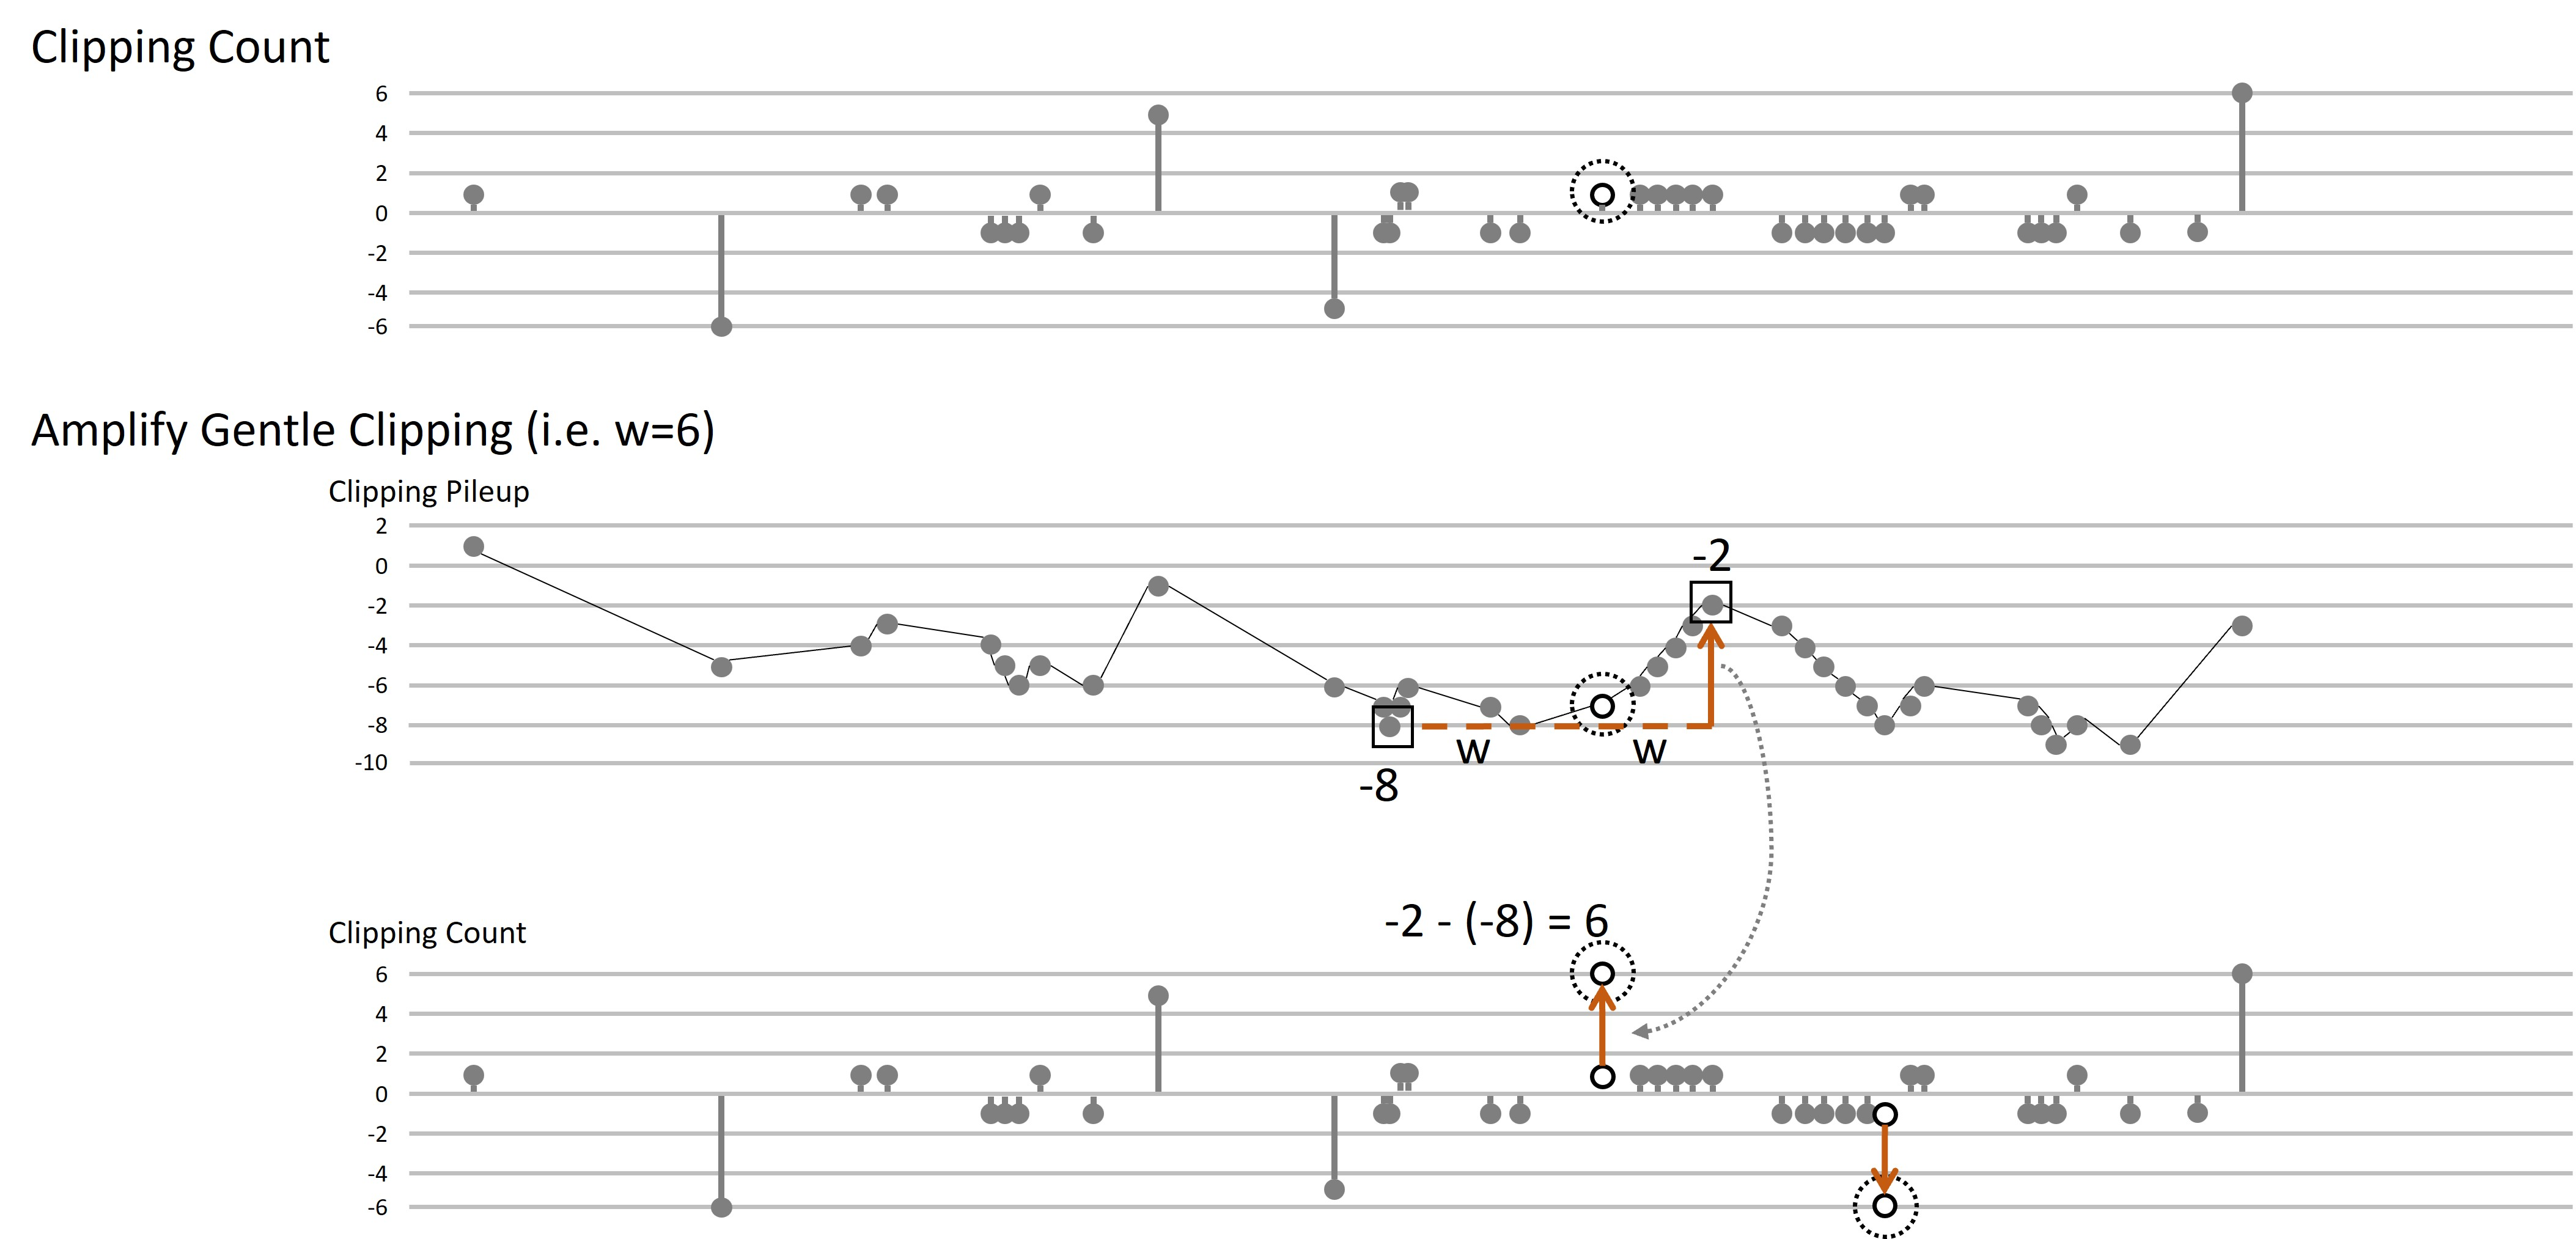
\includegraphics[keepaspectratio]{page_15_cropped.jpg}}
%   \caption[Boundary support from distributed clipping]{Support for each retained distributed-signal candidate is estimated from the difference between the smoothed cumulative clipping signal 10 clip-bearing positions downstream and upstream of the candidate. Positive and negative differences preserve the two clipping orientations for subsequent interval classification. The implementation smooths over 100 positions, whereas the schematic uses a six-position window for clarity.}\label{fig:met-page-15-cropped-jpg}
% \end{figure}
%
% \begin{figure}
%   \centering
%   \pandocbounded{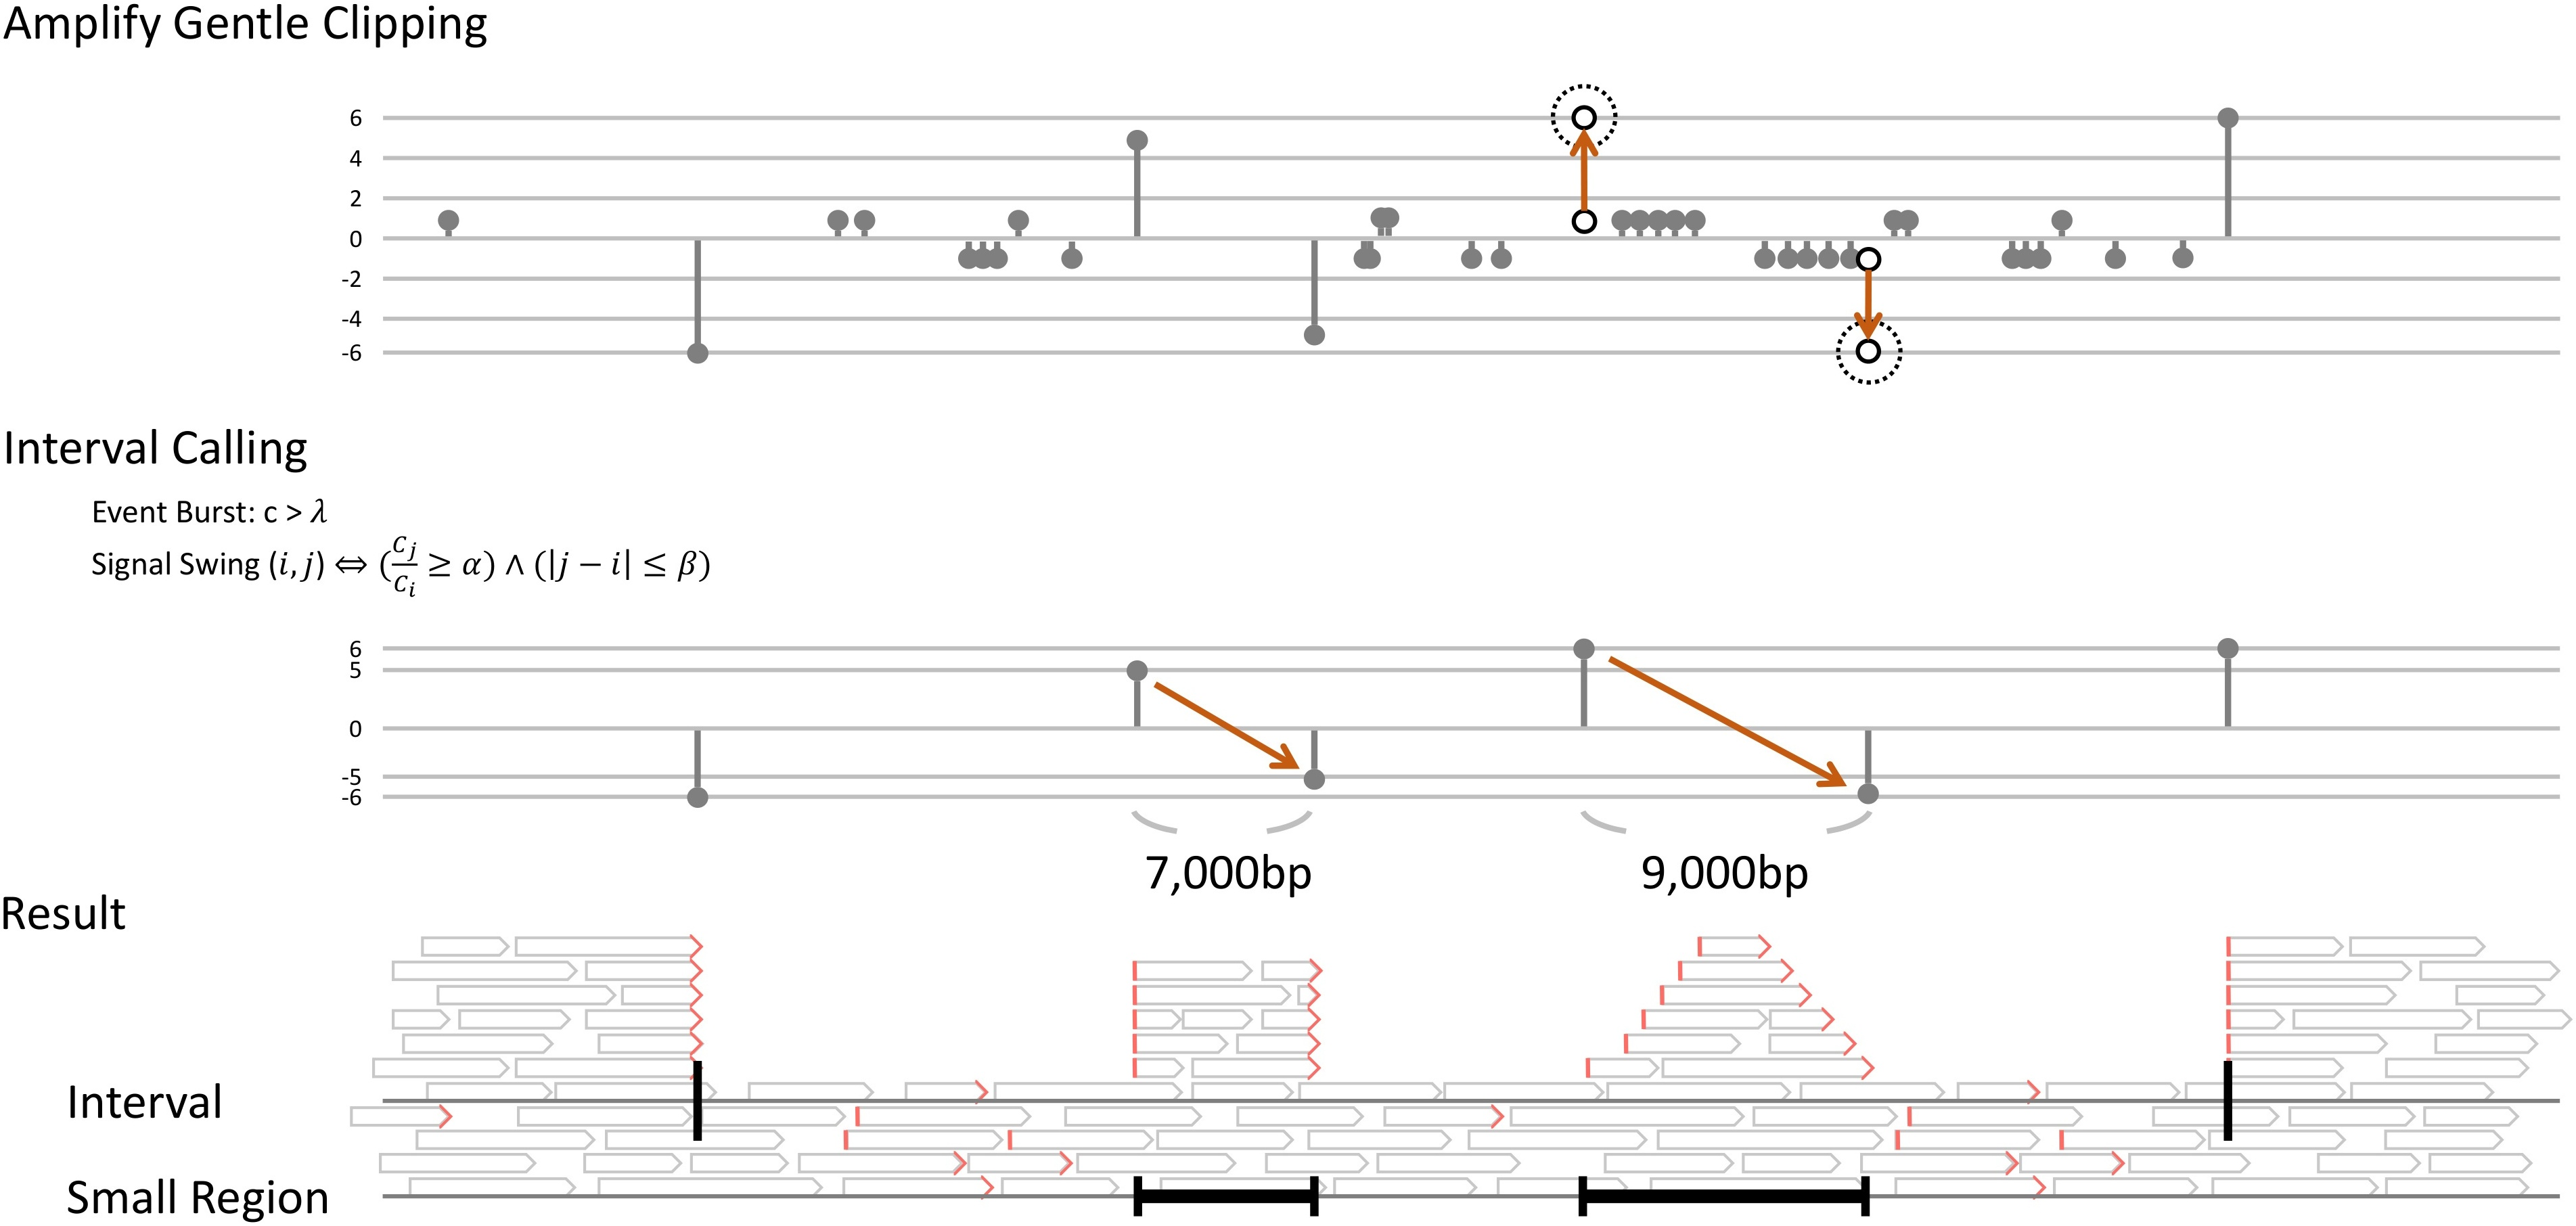
\includegraphics[keepaspectratio]{page_16_cropped.jpg}}
%   \caption[Breakpoint-associated interval calling]{A directional signal supported by at least five clips initiates a candidate event. An opposite-orientation signal within 10 kb completes a small-genomic-event (SGE) interval when its support reaches the integer one-quarter threshold relative to the maximum initiating-orientation support; otherwise, the initiating signal is retained as a large-genomic-event (LGE) boundary that partitions the chromosome for LOH evaluation. SGE and LGE are operational classes and do not assign a molecular event subtype.}\label{fig:met-page-16-cropped-jpg}
% \end{figure}

\begin{figure}
  \centering
  \pandocbounded{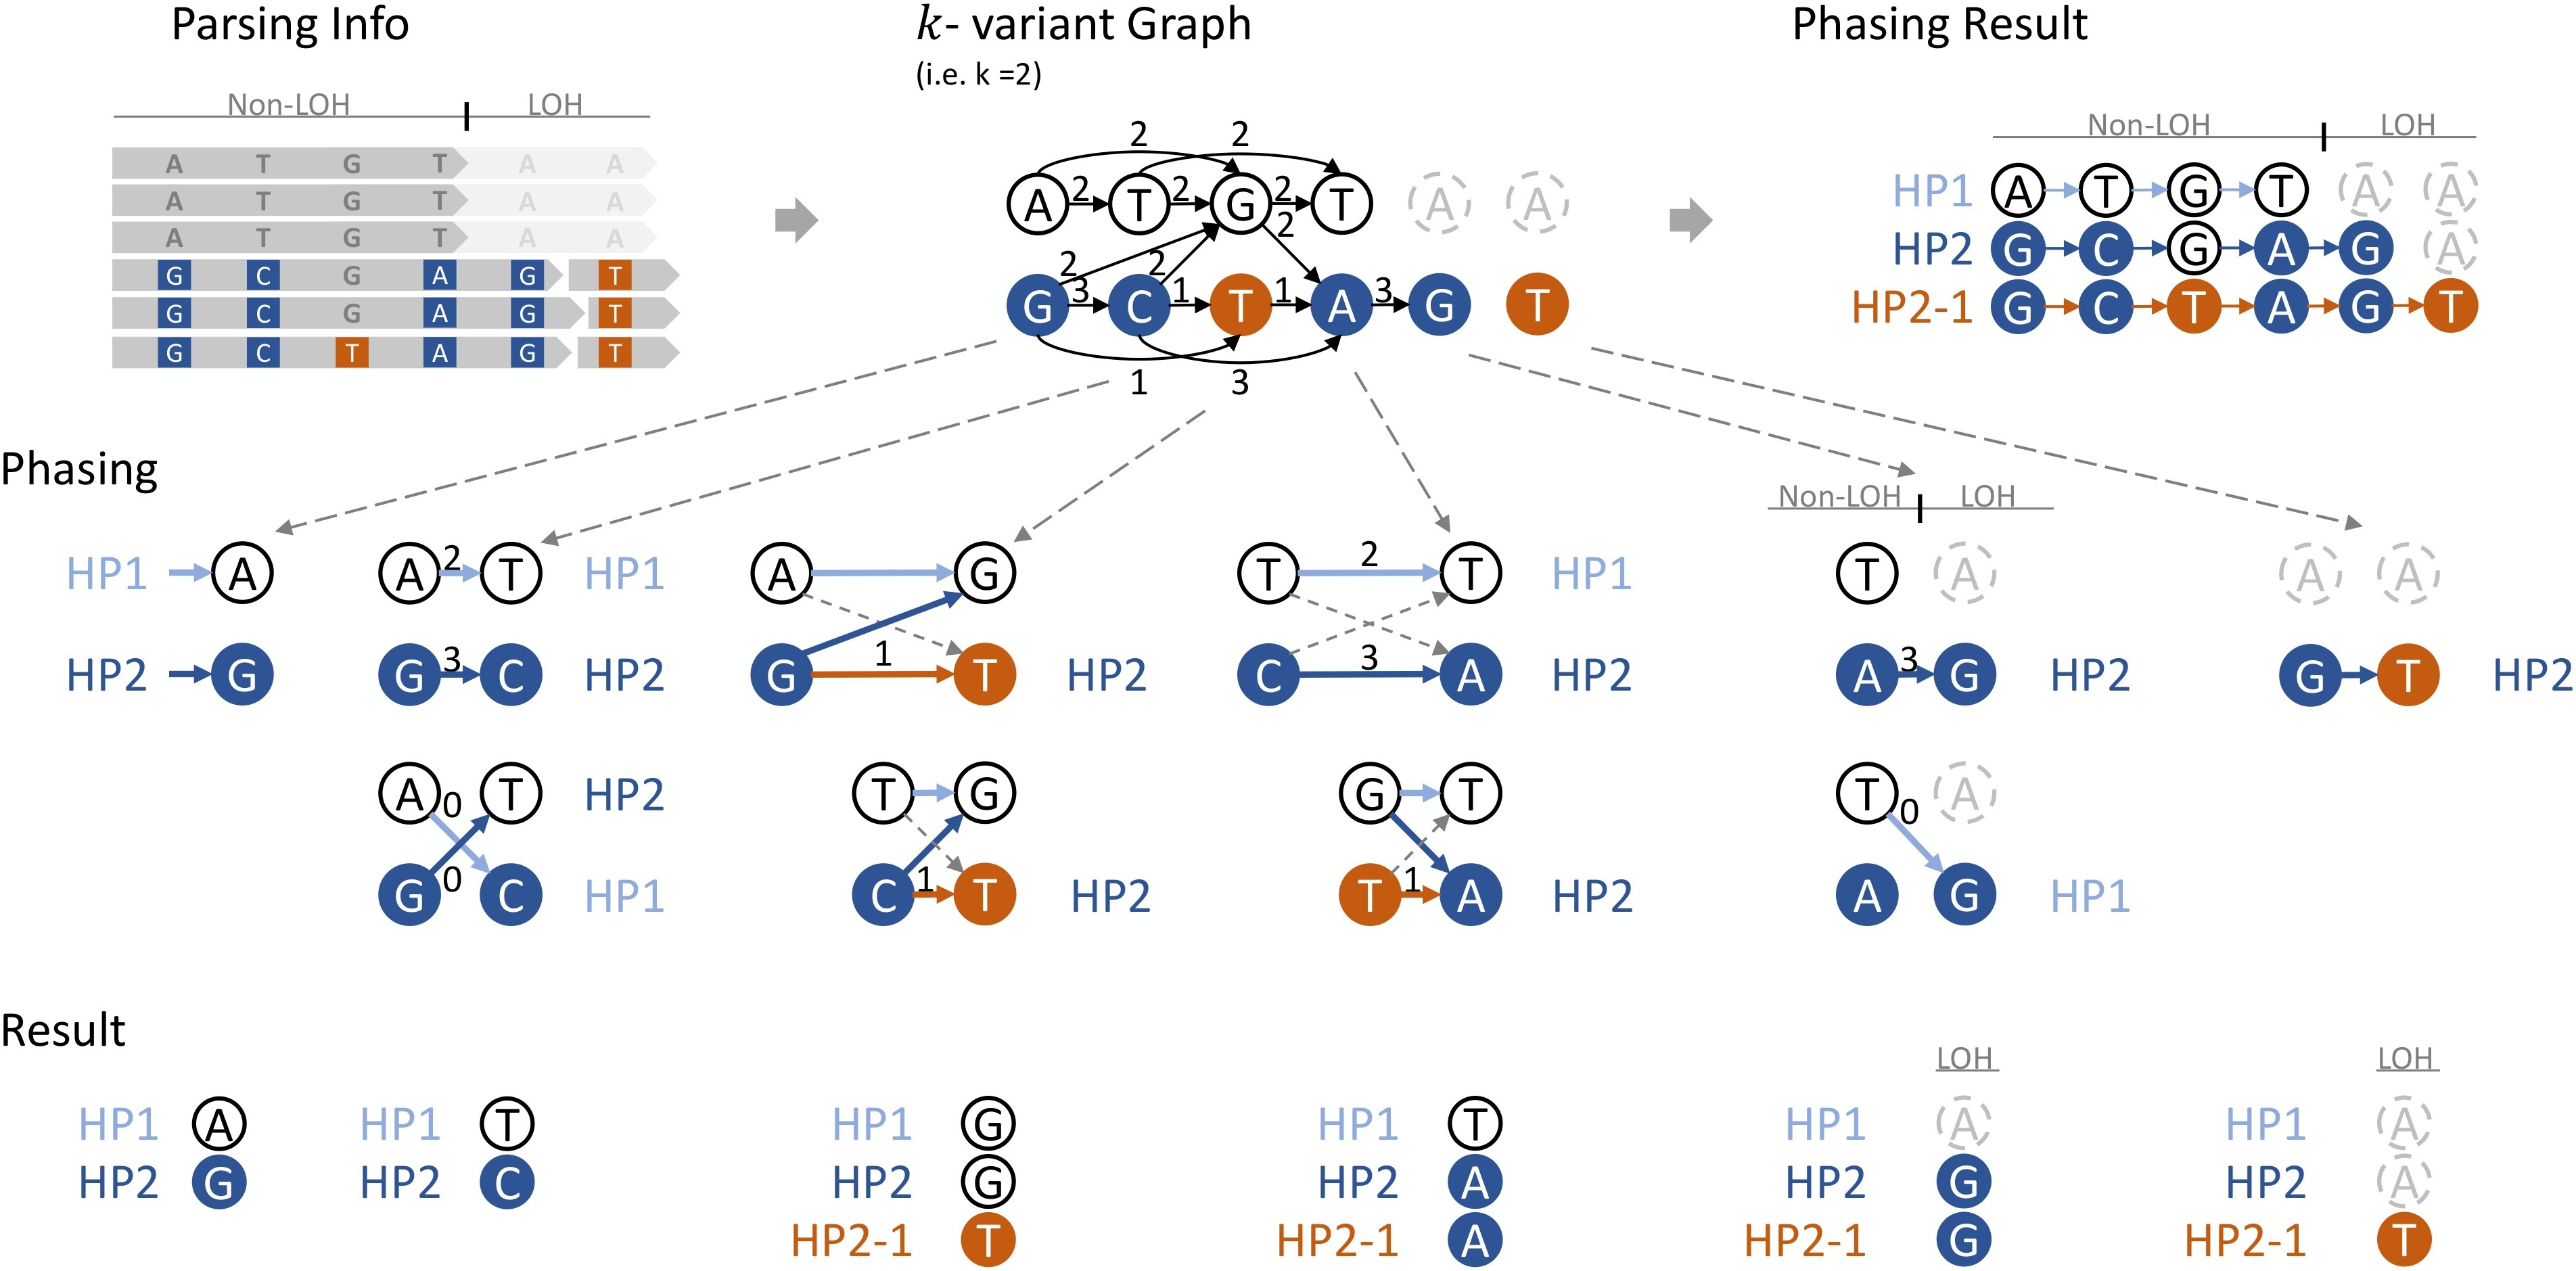
\includegraphics[keepaspectratio]{page_24_cropped.jpg}}
  \caption[Joint germline and somatic phasing across LOH]{Joint germline and somatic phasing across LOH. Read-level allele observations are converted into a local allele-linkage graph in which nodes represent reference or alternate alleles and weighted edges represent their co-occurrence on reads. Parallel and crossed linkage evidence is combined across neighboring variants to assign alleles to the parental haplotypes HP1 and HP2. A somatic alternate allele is assigned to its supporting parental haplotype and represented as a derived somatic haplotype, such as HP2-1. At an LOH boundary, read connections between flanking heterozygous variants and homozygous variants within the LOH segment identify the retained parental haplotype, and the lost path is shown in grey, whereas the retained parental and somatic paths continue through the LOH region. The schematic uses $k=2$ for clarity, and implementation details are provided in Supplementary Methods (Section~\ref{supp:loh-aware-phasing}).}\label{fig:met-page-24-cropped-jpg}
\end{figure}

\begin{figure}
  \centering
  \pandocbounded{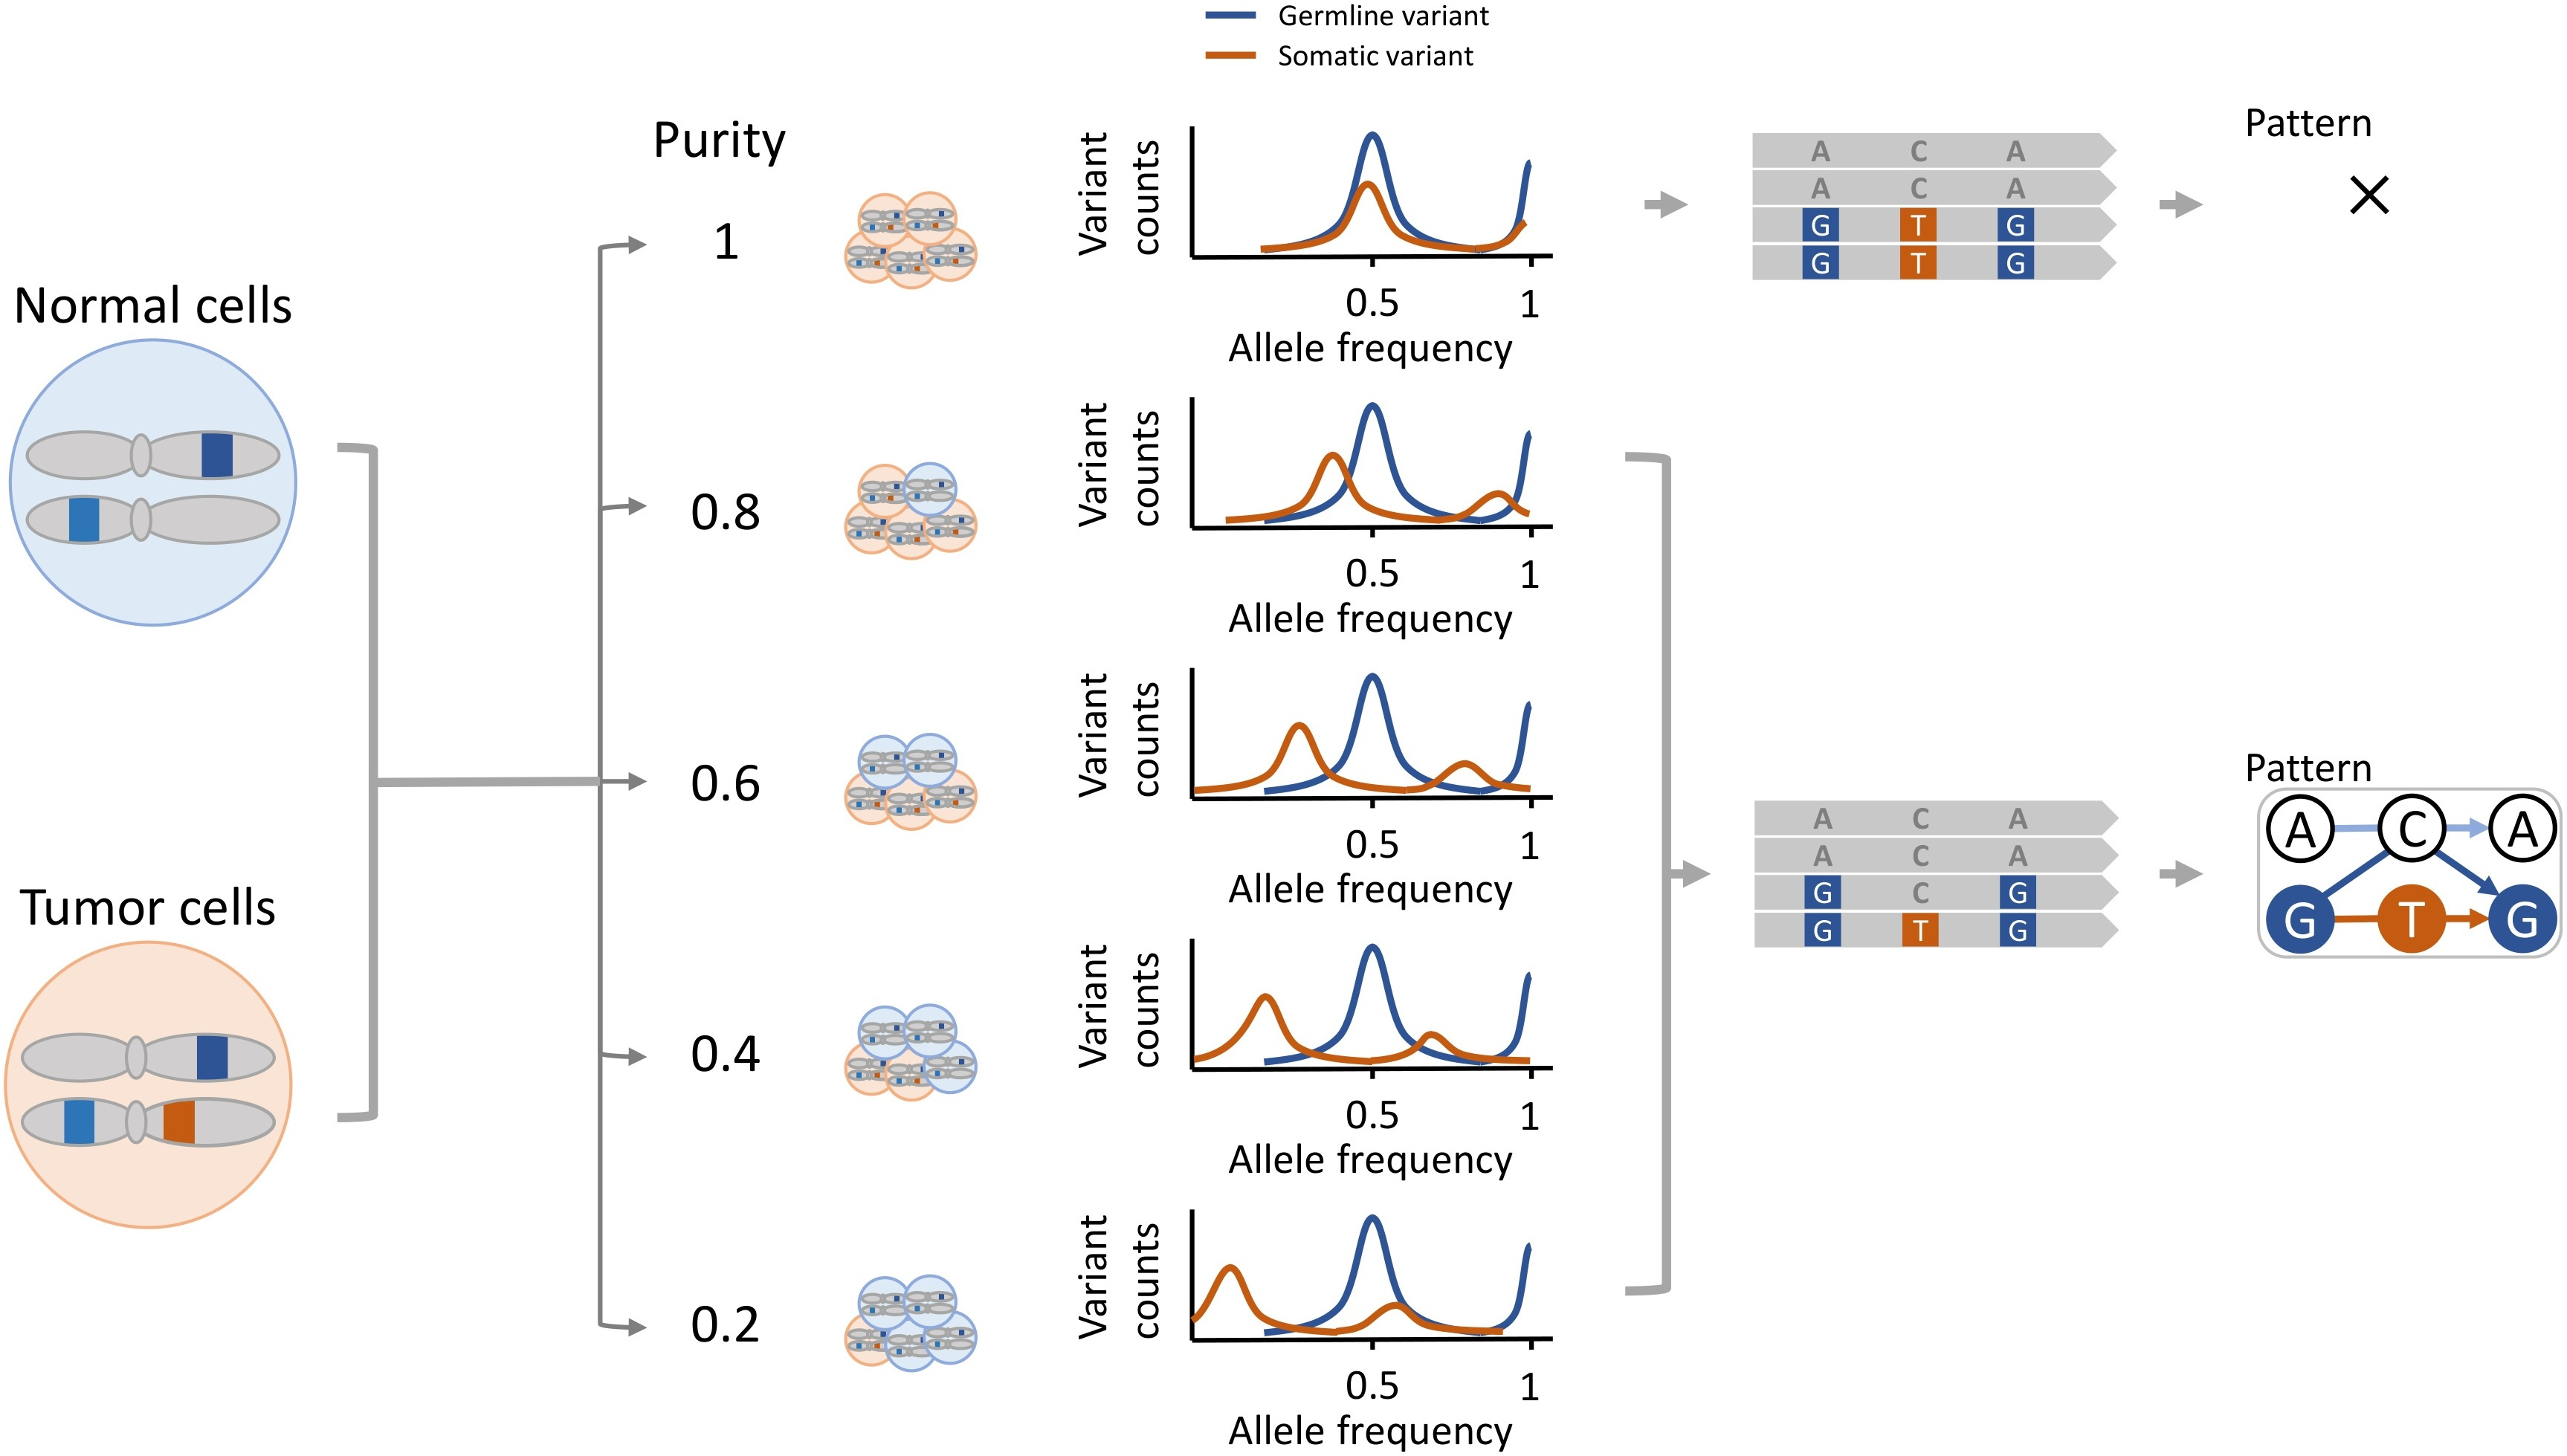
\includegraphics[keepaspectratio]{page_41_cropped.jpg}}
  \caption[Effect of tumor DNA fraction on allele frequencies]{Effect of tumor DNA fraction on variant allele frequencies (VAFs). The VAF of a heterozygous germline variant remains stable at approximately 0.5 across DNA fraction levels, whereas the VAF of a heterozygous somatic variant decreases proportionally with decreasing DNA fraction. At high DNA fraction, the distributions of somatic and germline variants overlap, complicating statistical separation.}\label{fig:app-page-41-cropped-jpg}
\end{figure}

\begin{figure}
  \centering
  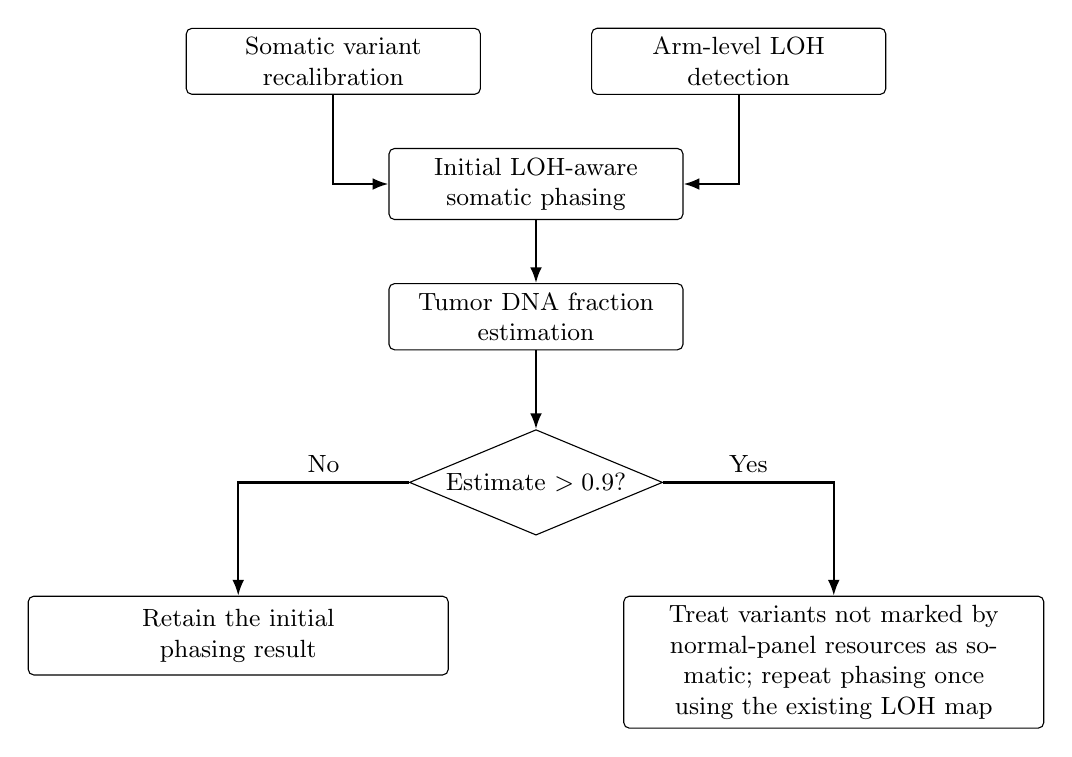
\begin{tikzpicture}[
    stage/.style={draw, rounded corners=2pt, align=center, minimum height=8mm, text width=35mm, font=\small},
    decision/.style={draw, diamond, aspect=2.4, align=center, inner sep=1.5pt, font=\small},
    branch/.style={draw, rounded corners=2pt, align=center, minimum height=10mm, text width=51mm, font=\small},
    flow/.style={-{Latex[length=2mm]}, thick},
    node distance=8mm and 14mm
  ]
    \node[stage] (recalibration) {Somatic variant\\recalibration};
    \node[stage, right=of recalibration] (loh) {Arm-level LOH\\detection};
    \coordinate (preparation) at ($(recalibration)!0.5!(loh)$);
    \node[stage, below=11mm of preparation] (phasing) {Initial LOH-aware\\somatic phasing};
    \node[stage, below=of phasing] (estimate) {Tumor DNA fraction\\estimation};
    \node[decision, below=10mm of estimate] (threshold) {Estimate $>0.9$?};
    \node[branch, below left=11mm and 3mm of threshold] (retain) {Retain the initial\\phasing result};
    \node[branch, below right=11mm and 3mm of threshold] (repeat) {Treat variants not marked by normal-panel resources as somatic; repeat phasing once using the existing LOH map};

    \draw[flow] (recalibration) |- (phasing);
    \draw[flow] (loh) |- (phasing);
    \draw[flow] (phasing) -- (estimate);
    \draw[flow] (estimate) -- (threshold);
    \draw[flow] (threshold) -| node[pos=0.25, above, font=\small] {No} (retain);
    \draw[flow] (threshold) -| node[pos=0.25, above, font=\small] {Yes} (repeat);
  \end{tikzpicture}
  \caption[Conditional second phasing pass]{Conditional second phasing pass for high-DNA-fraction samples. Somatic variant recalibration and arm-level LOH detection are completed before the initial LOH-aware phasing pass. When the resulting tumor DNA fraction estimate exceeds 0.9, variants not marked by the normal-panel resources are treated as somatic and phasing is repeated once using the existing LOH map. Otherwise, the initial phasing result is retained. The tumor DNA fraction is not re-estimated.}\label{fig:app-page-42-cropped-jpg}
\end{figure}

% The former haplotype-imbalance and tumor-DNA-fraction model schematics are
% commented out because their content is already presented in Figure 4(a,b).
% \begin{figure}
%   \centering
%   \pandocbounded{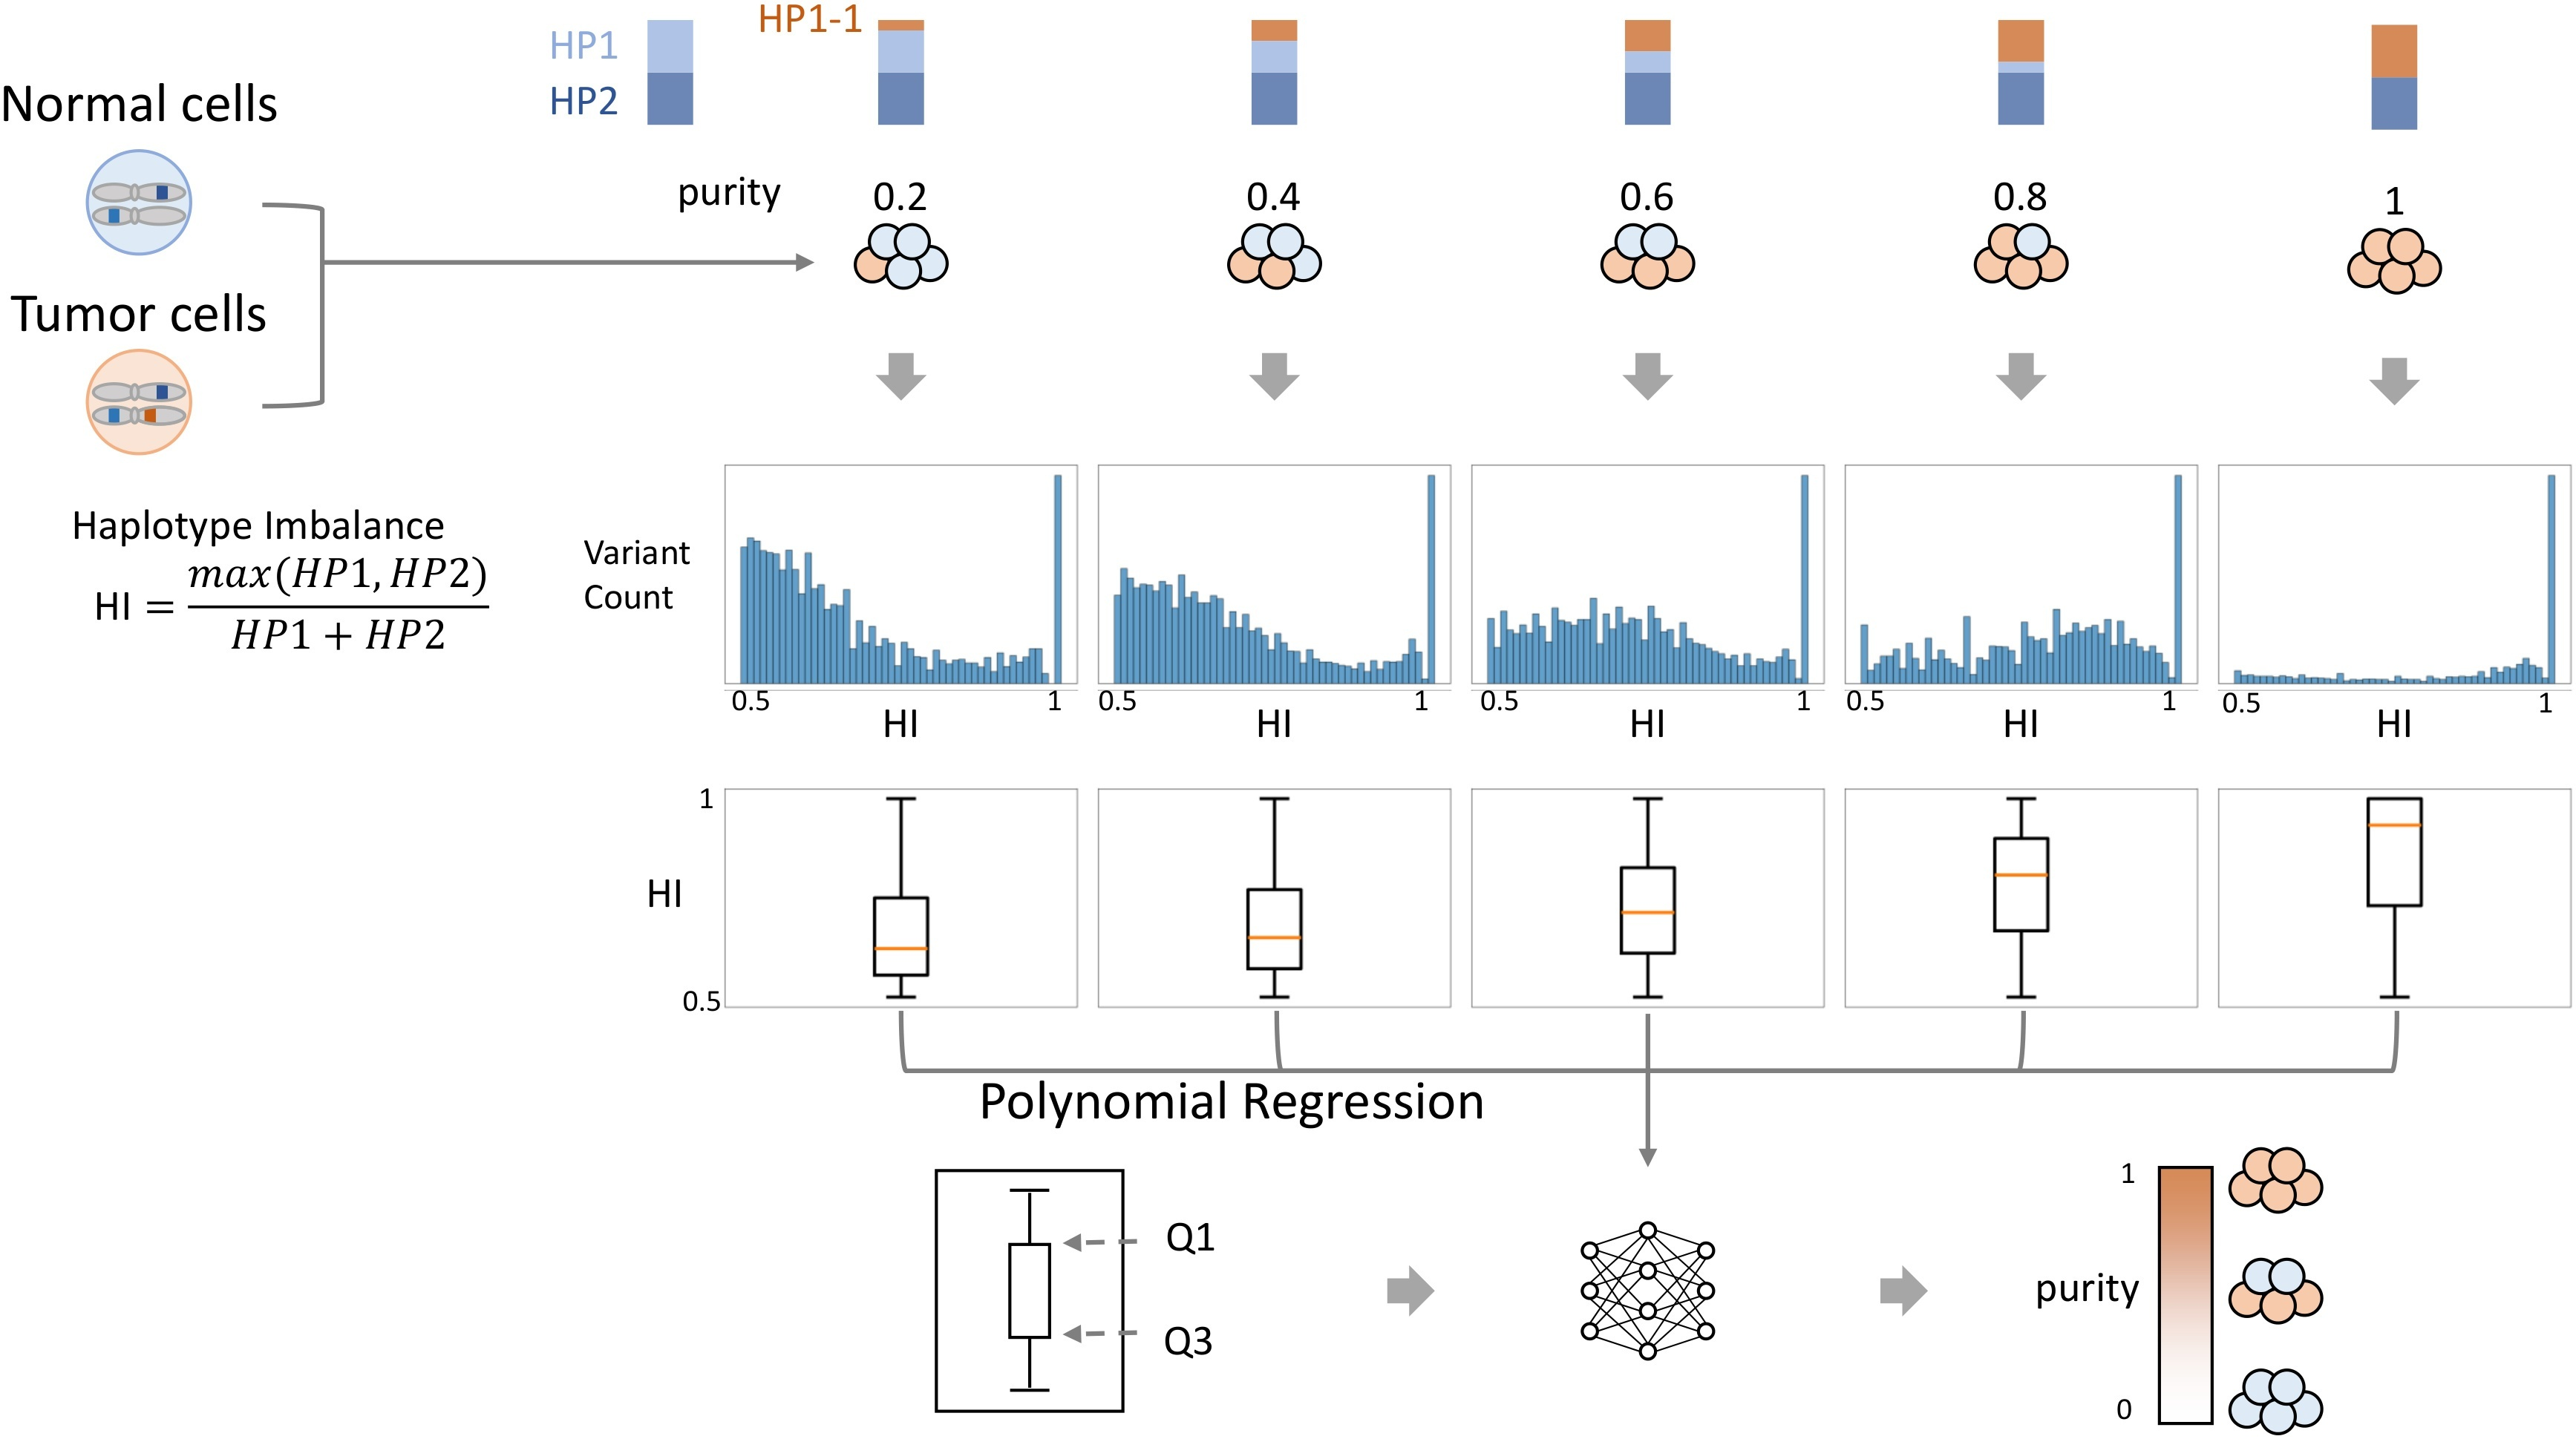
\includegraphics[keepaspectratio]{page_25_cropped.jpg}}
%   \caption[Haplotype Imbalance Principle]{Principle of tumor DNA fraction prediction using Haplotype Imbalance (HI). The figure shows that as tumor DNA fraction increases from 0.2 to 1.0, the proportion of somatic haplotypes increases. This causes the genome-wide distribution of HI, shown in histograms and box plots, to shift from a balanced state (centered at 0.5) to a highly imbalanced state with higher median values and a peak at 1.0.}\label{fig:met-page-25-cropped-jpg}
% \end{figure}
%
% \begin{figure}
%   \centering
%   \pandocbounded{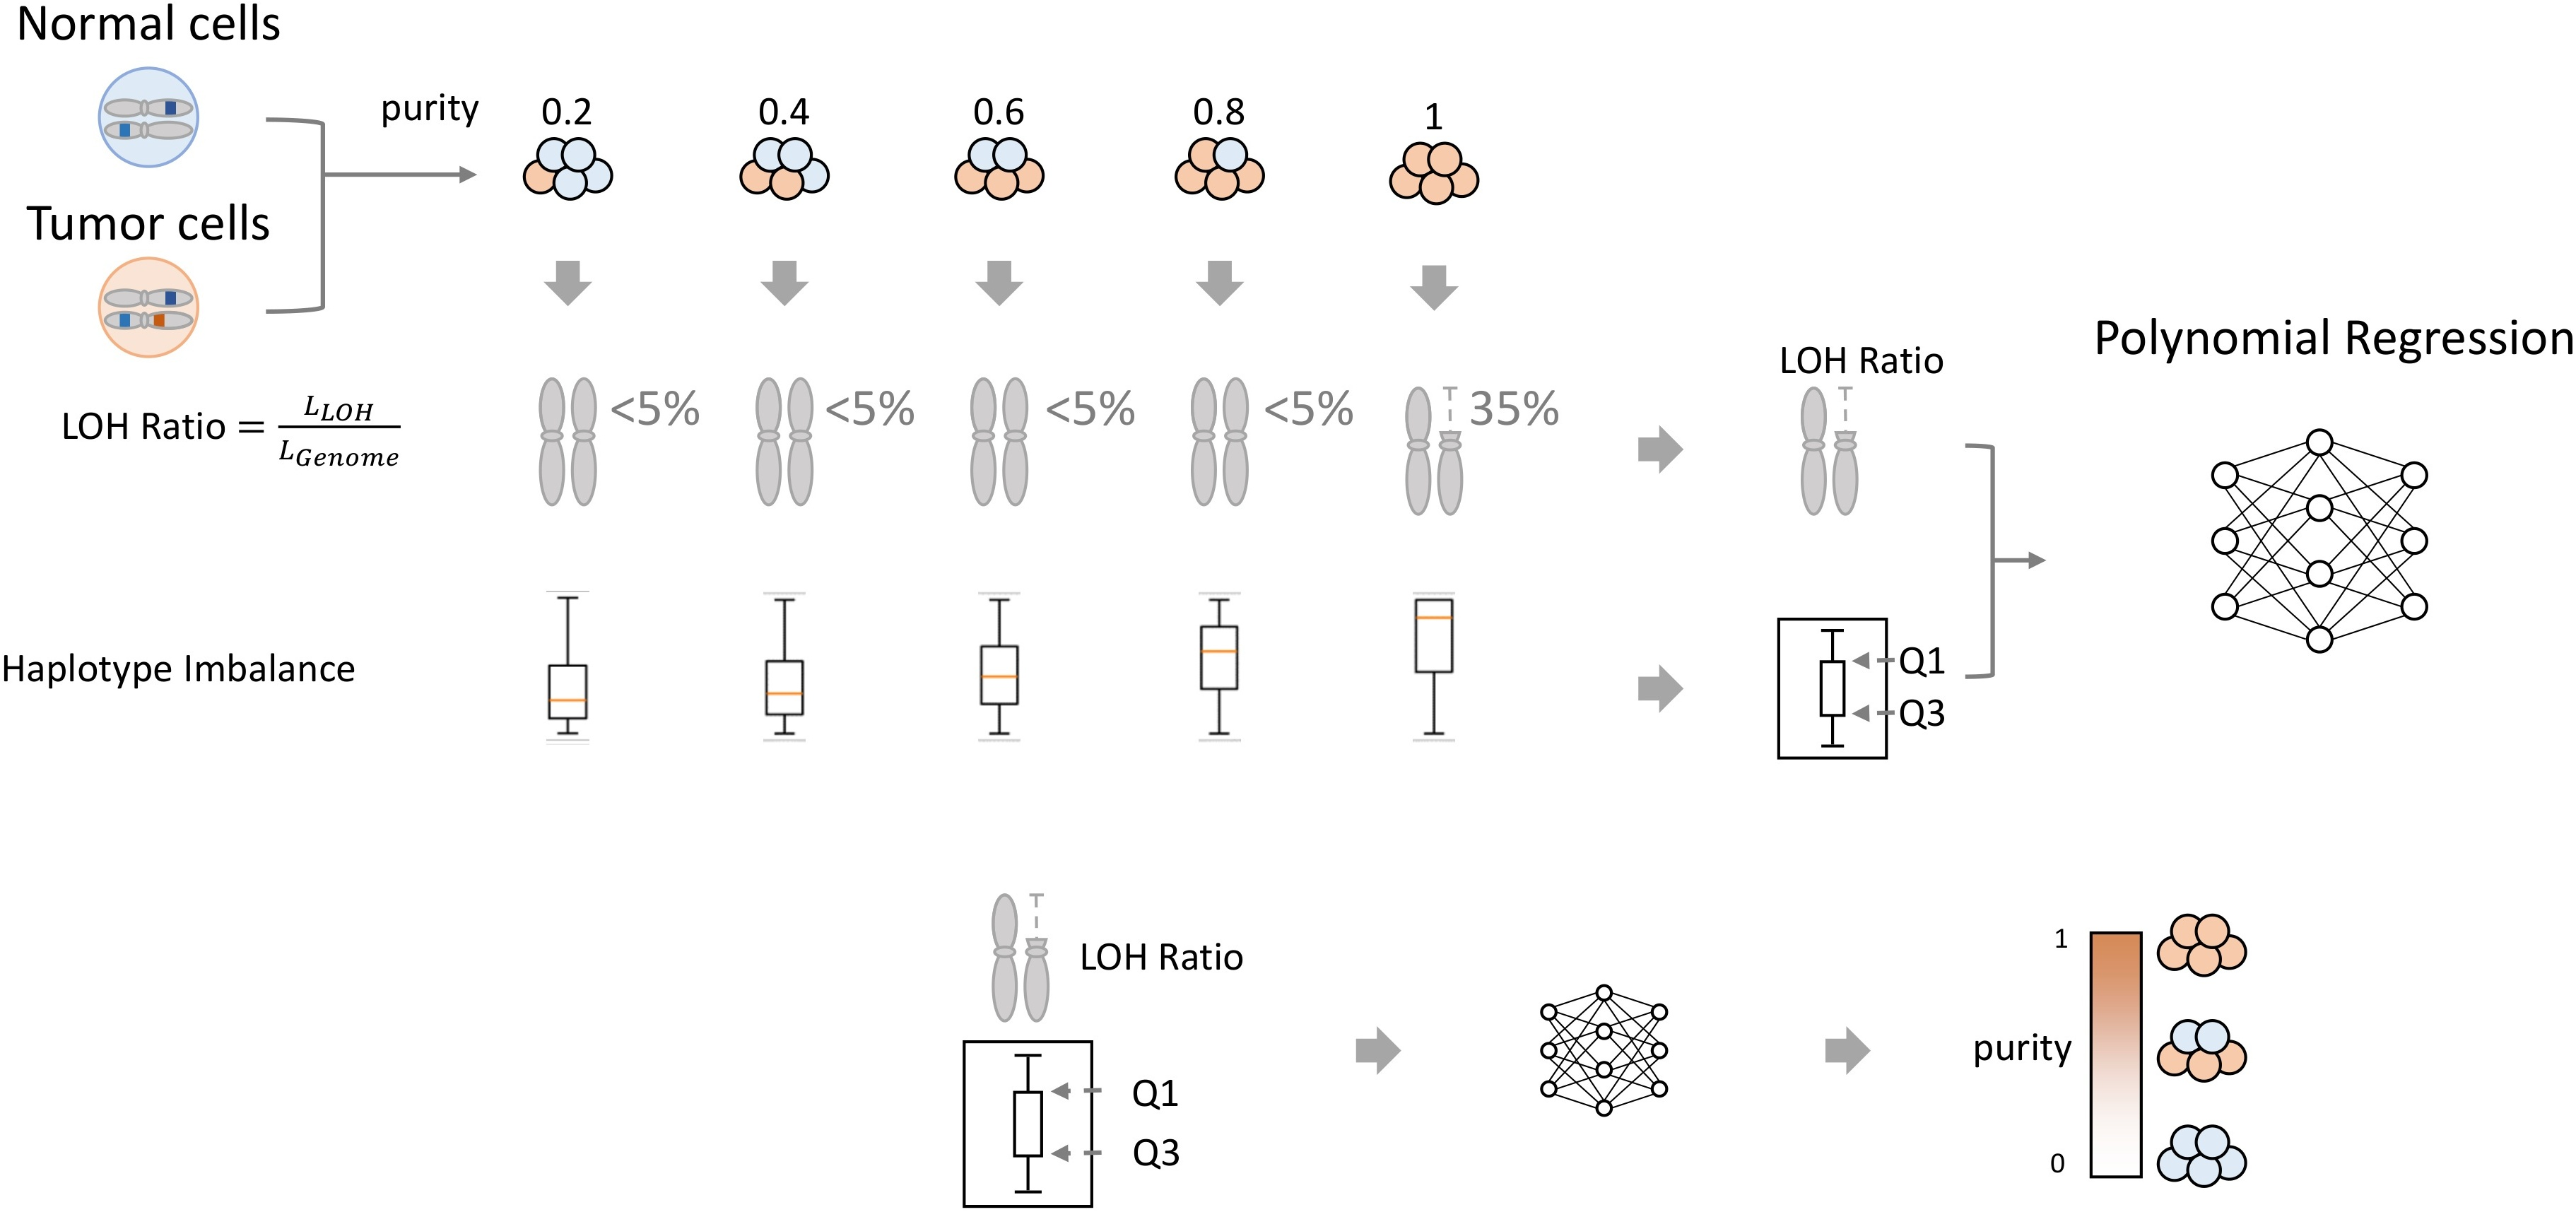
\includegraphics[keepaspectratio]{page_26_cropped.jpg}}
%   \caption[Tumor DNA Fraction Prediction Model]{Schematic of the tumor DNA fraction prediction model. The model takes two types of genomic features as input: the LOH Ratio (fraction of the genome with LOH) and statistics from the Haplotype Imbalance distribution (represented by the Q1 and Q3 quartiles of a box plot). These features are provided to a Polynomial Regression model, from which the estimated tumor DNA fraction is obtained.}\label{fig:met-page-26-cropped-jpg}
% \end{figure}

\clearpage

\section{Supplementary Tables}

{\small
\begin{longtable}{@{}llllll@{}}
  \caption[Nanopore cell-line datasets and benchmark sources with coverage]%
  {Nanopore cell-line datasets and corresponding benchmark truth sets, with normal and tumor coverages. All eight datasets were generated by Oxford Nanopore sequencing. The Source column names the group that produced the reads (HKU, NYGC, ONT or UCSC) and not the sequencing platform, and the Benchmark column names the origin of the somatic truth set (SEQC2, NYGC or DeepSomatic). In particular, COLO829\_NYGC denotes nanopore reads produced by NYGC, evaluated against the NYGC somatic truth set.}
  \label{tab:cell-line-datasets-and-benchmark-sources}\\
  \toprule
  Dataset & Cancer type & Source & Benchmark & Normal coverage & Tumor coverage \\
  \midrule
  \endfirsthead
  \toprule
  Dataset & Cancer type & Source & Benchmark & Normal coverage & Tumor coverage \\
  \midrule
  \endhead
  \bottomrule
  \endlastfoot
  HCC1395\_HKU   & Breast ductal carcinoma                & HKU  & SEQC2       & 45.70$\times$ & 76.27$\times$ \\
  HCC1395\_NYGC  & Breast ductal carcinoma                & NYGC & SEQC2       & 29.14$\times$ & 79.52$\times$ \\
  COLO829\_ONT   & Malignant melanoma                     & ONT  & NYGC        & 39.83$\times$ & 33.45$\times$ \\
  COLO829\_NYGC  & Malignant melanoma                     & NYGC & NYGC        & 45.85$\times$ & 108.49$\times$ \\
  HCC1954\_UCSC  & Breast ductal carcinoma                & UCSC & DeepSomatic & 34.03$\times$ & 82.44$\times$ \\
  HCC1937\_UCSC  & Breast ductal carcinoma                & UCSC & DeepSomatic & 25.68$\times$ & 158.44$\times$ \\
  H2009\_UCSC    & Non-small-cell lung cancer             & UCSC & DeepSomatic & 30.07$\times$ & 106.92$\times$ \\
  H1437\_UCSC    & Non-small-cell lung cancer             & UCSC & DeepSomatic & 49.28$\times$ & 79.10$\times$ \\
\end{longtable}
}

\begin{table}[htbp]
  \centering
  \caption[Comparison of phasing tools]%
  {Comparison of conventional phasing tools with LongPhase-TO.}
  \label{tab:phasing-performance}
  \begin{tabular}{@{}llrrrr@{}}
    \toprule
    Sample & Phasing tool & Phased ratio & Blocks & Block N50 (bp) & Block sum (bp) \\
    \midrule
    COLO829\_ONT & HapCUT2      & 0.531 & 3569  & 4645832  & 2523260676 \\
    COLO829\_ONT & WhatsHap     & 0.530 & 3686  & 4635320  & 2518385299 \\
    COLO829\_ONT & LongPhase    & 0.498 & 3477  & 4887010  & 2540883450 \\
    COLO829\_ONT & LongPhase-TO & 0.594 & 1110  & 9852371  & 2835034563 \\
    \addlinespace
    COLO829\_NYGC & HapCUT2      & 0.557 & 15016 & 584415   & 2187808909 \\
    COLO829\_NYGC & WhatsHap     & 0.556 & 15261 & 575997   & 2182781406 \\
    COLO829\_NYGC & LongPhase    & 0.521 & 15017 & 570504   & 2176223422 \\
    COLO829\_NYGC & LongPhase-TO & 0.607 & 6576  & 1403687  & 2664715137 \\
    \addlinespace
    H1437\_UCSC & HapCUT2      & 0.540 & 2376  & 7048644  & 2625509787 \\
    H1437\_UCSC & WhatsHap     & 0.539 & 2398  & 7048644  & 2624731180 \\
    H1437\_UCSC & LongPhase    & 0.502 & 2287  & 7729758  & 2654323753 \\
    H1437\_UCSC & LongPhase-TO & 0.698 & 529   & 19323318 & 2864794192 \\
    \addlinespace
    H2009\_UCSC & HapCUT2      & 0.557 & 2252  & 5825292  & 2677986524 \\
    H2009\_UCSC & WhatsHap     & 0.556 & 2292  & 5723430  & 2676922405 \\
    H2009\_UCSC & LongPhase    & 0.517 & 2204  & 7217802  & 2706782369 \\
    H2009\_UCSC & LongPhase-TO & 0.682 & 638   & 23169348 & 2863280796 \\
    \addlinespace
    HCC1395\_HKU & HapCUT2      & 0.602 & 4553  & 1678506  & 2536199864 \\
    HCC1395\_HKU & WhatsHap     & 0.600 & 4662  & 1667777  & 2532455755 \\
    HCC1395\_HKU & LongPhase    & 0.561 & 4581  & 1754642  & 2569265774 \\
    HCC1395\_HKU & LongPhase-TO & 0.576 & 893   & 16768123 & 2847723783 \\
    \addlinespace
    HCC1395\_NYGC & HapCUT2      & 0.499 & 21138 & 275106   & 1972073127 \\
    HCC1395\_NYGC & WhatsHap     & 0.498 & 21510 & 270769   & 1966798050 \\
    HCC1395\_NYGC & LongPhase    & 0.468 & 21057 & 279702   & 1980748528 \\
    HCC1395\_NYGC & LongPhase-TO & 0.693 & 5227  & 13441849 & 2726465382 \\
    \addlinespace
    HCC1937\_UCSC & HapCUT2      & 0.402 & 4537  & 1447908  & 2430726898 \\
    HCC1937\_UCSC & WhatsHap     & 0.401 & 4650  & 1420186  & 2425582425 \\
    HCC1937\_UCSC & LongPhase    & 0.375 & 4517  & 1513047  & 2454370721 \\
    HCC1937\_UCSC & LongPhase-TO & 0.713 & 1135  & 25207324 & 2830053891 \\
    \addlinespace
    HCC1954\_UCSC & HapCUT2      & 0.652 & 1969  & 5927639  & 2711566888 \\
    HCC1954\_UCSC & WhatsHap     & 0.650 & 1999  & 5908073  & 2710095182 \\
    HCC1954\_UCSC & LongPhase    & 0.610 & 1923  & 5912510  & 2736740481 \\
    HCC1954\_UCSC & LongPhase-TO & 0.659 & 1115  & 6477286  & 2828110080 \\
    \bottomrule
  \end{tabular}
\end{table}

\begin{table}[htbp]
  \centering\footnotesize
  \caption[Loss of heterozygosity summary metrics]%
  {Loss of heterozygosity (LOH) summary metrics across samples and methods. Entries marked n.a.\ indicate that the method returned no estimate.}
  \label{tab:loh_summary}
  \begin{tabular}{@{}llrrrr@{}}
    \toprule
    Sample & LOH method & LOH burden (\%) & Blocks & LOH sum (bp) & LOH N50 (bp) \\
    \midrule
    COLO829\_ONT   & ASCAT (T+N)                  & 35.33 & 575  & 1015662001 & 12864314  \\
    COLO829\_ONT   & ASCAT (TO)                   & 39.31 & 290  & 1130080160 & 20362317  \\
    COLO829\_ONT   & LongPhase-TO (ClairS-TO)      & 26.85 &  90  &  771811167 & 50760310  \\
    COLO829\_ONT   & LongPhase-TO (DeepSomatic-TO) & 27.10 & 105  &  779127888 & 50760310  \\
    COLO829\_NYGC  & ASCAT (T+N)                  & 29.11 &  45  &  836961836 & 80866668  \\
    COLO829\_NYGC  & ASCAT (TO)                   & 33.24 & 192  &  955772886 & 38166624  \\
    COLO829\_NYGC  & LongPhase-TO (ClairS-TO)      & 28.11 & 119  &  808144053 & 35105161  \\
    COLO829\_NYGC  & LongPhase-TO (DeepSomatic-TO) & 29.05 & 159  &  835138542 & 45643569 \\
    H1437\_UCSC    & ASCAT (T+N)                  & 39.51 & 1948 & 1135872591 &  3829891  \\
    H1437\_UCSC    & ASCAT (TO)                   & 44.70 & 531  & 1285175995 & 34097583  \\
    H1437\_UCSC    & LongPhase-TO (ClairS-TO)      & 34.62 & 128  &  995275823 & 43336933  \\
    H1437\_UCSC    & LongPhase-TO (DeepSomatic-TO) & 34.79 & 125  & 1000311306 & 34605403  \\
    H2009\_UCSC    & ASCAT (T+N)                  & 43.39 & 1553 & 1247558196 &  4110937  \\
    H2009\_UCSC    & ASCAT (TO)                   & 48.26 & 721  & 1387574137 &  9209663  \\
    H2009\_UCSC    & LongPhase-TO (ClairS-TO)      & 35.93 & 127  & 1033104502 & 31122631  \\
    H2009\_UCSC    & LongPhase-TO (DeepSomatic-TO) & 36.09 & 147  & 1037482232 & 34937899  \\
    HCC1395\_HKU   & ASCAT (T+N)                  & 52.01 & 3068 & 1495294320 &  2803775  \\
    HCC1395\_HKU   & ASCAT (TO)                   & 65.72 & 1392 & 1889479858 &  6023307  \\
    HCC1395\_HKU   & LongPhase-TO (ClairS-TO)      & 50.84 & 198  & 1461681845 & 21772604  \\
    HCC1395\_HKU   & LongPhase-TO (DeepSomatic-TO) & 51.53 & 202  & 1481487680 & 21597183  \\
    HCC1395\_NYGC  & ASCAT (T+N)                  & 52.69 & 2134 & 1514982034 &  9642863  \\
    HCC1395\_NYGC  & ASCAT (TO)                   & 59.07 & 584  & 1698371776 & 16795656  \\
    HCC1395\_NYGC  & LongPhase-TO (ClairS-TO)      & 50.74 & 220  & 1458689344 & 26501707  \\
    HCC1395\_NYGC  & LongPhase-TO (DeepSomatic-TO) & 51.86 & 253  & 1490967218 & 29068243  \\
    HCC1937\_UCSC  & ASCAT (T+N)                  & 60.44 & 4483 & 1737671187 &  2214193  \\
    HCC1937\_UCSC  & ASCAT (TO)                   & 62.07 & 389  & 1784605418 & 20879693  \\
    HCC1937\_UCSC  & LongPhase-TO (ClairS-TO)      & 55.86 & 169  & 1606116347 & 40921298  \\
    HCC1937\_UCSC  & LongPhase-TO (DeepSomatic-TO) & 56.05 & 170  & 1611305118 & 43800261  \\
    HCC1954\_UCSC  & ASCAT (T+N)                  & n.a. & n.a. & n.a. & n.a. \\
    HCC1954\_UCSC  & ASCAT (TO)                   & 58.72 & 1341 & 1688216927 &  2812944  \\
    HCC1954\_UCSC  & LongPhase-TO (ClairS-TO)      & 9.55 & 147  &  274660981 & 16263599  \\
    HCC1954\_UCSC  & LongPhase-TO (DeepSomatic-TO) & 10.28 & 165  &  295496102 & 15126962  \\
    \bottomrule
  \end{tabular}
\end{table}

\FloatBarrier
{\small
\begin{longtable}{@{}lllccc@{}}
  \caption[Somatic SNV calling performance across DNA fraction levels]%
  {Somatic SNV calling performance across DNA fraction levels for eight tumor cell line
  datasets. Fraction is the tumor DNA fraction.}
  \label{tab:somatic_purity}\\
  \toprule
  Sample & Fraction & Variant caller & Precision & Recall & F1-score \\
  \midrule
  \endfirsthead
  \toprule
  Sample & Fraction & Variant caller & Precision & Recall & F1-score \\
  \midrule
  \endhead
  \bottomrule
  \endlastfoot
  COLO829\_ONT & 1 & ClairS-TO & 0.674 & 0.799 & 0.731 \\
  COLO829\_ONT & 1 & ClairS-TO+LongPhase-TO & 0.666 & 0.808 & 0.730 \\
  COLO829\_ONT & 1 & DeepSomatic-TO & 0.501 & 0.844 & 0.629 \\
  COLO829\_ONT & 1 & DeepSomatic-TO+LongPhase-TO & 0.627 & 0.813 & 0.708 \\
  COLO829\_ONT & 0.8 & ClairS-TO & 0.651 & 0.790 & 0.714 \\
  COLO829\_ONT & 0.8 & ClairS-TO+LongPhase-TO & 0.853 & 0.680 & 0.757 \\
  COLO829\_ONT & 0.8 & DeepSomatic-TO & 0.481 & 0.849 & 0.614 \\
  COLO829\_ONT & 0.8 & DeepSomatic-TO+LongPhase-TO & 0.812 & 0.648 & 0.721 \\
  COLO829\_ONT & 0.6 & ClairS-TO & 0.623 & 0.764 & 0.686 \\
  COLO829\_ONT & 0.6 & ClairS-TO+LongPhase-TO & 0.842 & 0.750 & 0.793 \\
  COLO829\_ONT & 0.6 & DeepSomatic-TO & 0.466 & 0.842 & 0.600 \\
  COLO829\_ONT & 0.6 & DeepSomatic-TO+LongPhase-TO & 0.812 & 0.759 & 0.785 \\
  COLO829\_ONT & 0.4 & ClairS-TO & 0.576 & 0.659 & 0.615 \\
  COLO829\_ONT & 0.4 & ClairS-TO+LongPhase-TO & 0.808 & 0.667 & 0.731 \\
  COLO829\_ONT & 0.4 & DeepSomatic-TO & 0.445 & 0.797 & 0.571 \\
  COLO829\_ONT & 0.4 & DeepSomatic-TO+LongPhase-TO & 0.786 & 0.731 & 0.757 \\
  COLO829\_ONT & 0.2 & ClairS-TO & 0.392 & 0.326 & 0.356 \\
  COLO829\_ONT & 0.2 & ClairS-TO+LongPhase-TO & 0.660 & 0.352 & 0.459 \\
  COLO829\_ONT & 0.2 & DeepSomatic-TO & 0.373 & 0.604 & 0.461 \\
  COLO829\_ONT & 0.2 & DeepSomatic-TO+LongPhase-TO & 0.711 & 0.547 & 0.618 \\
  COLO829\_NYGC & 1 & ClairS-TO & 0.682 & 0.817 & 0.744 \\
  COLO829\_NYGC & 1 & ClairS-TO+LongPhase-TO & 0.677 & 0.830 & 0.746 \\
  COLO829\_NYGC & 1 & DeepSomatic-TO & 0.543 & 0.857 & 0.665 \\
  COLO829\_NYGC & 1 & DeepSomatic-TO+LongPhase-TO & 0.650 & 0.830 & 0.729 \\
  COLO829\_NYGC & 0.8 & ClairS-TO & 0.659 & 0.809 & 0.726 \\
  COLO829\_NYGC & 0.8 & ClairS-TO+LongPhase-TO & 0.857 & 0.652 & 0.741 \\
  COLO829\_NYGC & 0.8 & DeepSomatic-TO & 0.514 & 0.863 & 0.644 \\
  COLO829\_NYGC & 0.8 & DeepSomatic-TO+LongPhase-TO & 0.843 & 0.603 & 0.703 \\
  COLO829\_NYGC & 0.6 & ClairS-TO & 0.632 & 0.782 & 0.699 \\
  COLO829\_NYGC & 0.6 & ClairS-TO+LongPhase-TO & 0.851 & 0.697 & 0.766 \\
  COLO829\_NYGC & 0.6 & DeepSomatic-TO & 0.494 & 0.853 & 0.625 \\
  COLO829\_NYGC & 0.6 & DeepSomatic-TO+LongPhase-TO & 0.828 & 0.676 & 0.744 \\
  COLO829\_NYGC & 0.4 & ClairS-TO & 0.588 & 0.680 & 0.631 \\
  COLO829\_NYGC & 0.4 & ClairS-TO+LongPhase-TO & 0.817 & 0.627 & 0.710 \\
  COLO829\_NYGC & 0.4 & DeepSomatic-TO & 0.471 & 0.813 & 0.596 \\
  COLO829\_NYGC & 0.4 & DeepSomatic-TO+LongPhase-TO & 0.798 & 0.658 & 0.721 \\
  COLO829\_NYGC & 0.2 & ClairS-TO & 0.405 & 0.339 & 0.369 \\
  COLO829\_NYGC & 0.2 & ClairS-TO+LongPhase-TO & 0.674 & 0.331 & 0.444 \\
  COLO829\_NYGC & 0.2 & DeepSomatic-TO & 0.394 & 0.620 & 0.482 \\
  COLO829\_NYGC & 0.2 & DeepSomatic-TO+LongPhase-TO & 0.720 & 0.489 & 0.582 \\
  H1437\_UCSC & 1 & ClairS-TO & 0.770 & 0.588 & 0.667 \\
  H1437\_UCSC & 1 & ClairS-TO+LongPhase-TO & 0.768 & 0.596 & 0.671 \\
  H1437\_UCSC & 1 & DeepSomatic-TO & 0.680 & 0.620 & 0.649 \\
  H1437\_UCSC & 1 & DeepSomatic-TO+LongPhase-TO & 0.733 & 0.596 & 0.658 \\
  H1437\_UCSC & 0.8 & ClairS-TO & 0.728 & 0.558 & 0.632 \\
  H1437\_UCSC & 0.8 & ClairS-TO+LongPhase-TO & 0.874 & 0.530 & 0.660 \\
  H1437\_UCSC & 0.8 & DeepSomatic-TO & 0.624 & 0.620 & 0.622 \\
  H1437\_UCSC & 0.8 & DeepSomatic-TO+LongPhase-TO & 0.844 & 0.520 & 0.643 \\
  H1437\_UCSC & 0.6 & ClairS-TO & 0.721 & 0.533 & 0.613 \\
  H1437\_UCSC & 0.6 & ClairS-TO+LongPhase-TO & 0.834 & 0.556 & 0.667 \\
  H1437\_UCSC & 0.6 & DeepSomatic-TO & 0.603 & 0.607 & 0.605 \\
  H1437\_UCSC & 0.6 & DeepSomatic-TO+LongPhase-TO & 0.837 & 0.564 & 0.674 \\
  H1437\_UCSC & 0.4 & ClairS-TO & 0.730 & 0.483 & 0.581 \\
  H1437\_UCSC & 0.4 & ClairS-TO+LongPhase-TO & 0.808 & 0.501 & 0.619 \\
  H1437\_UCSC & 0.4 & DeepSomatic-TO & 0.584 & 0.570 & 0.577 \\
  H1437\_UCSC & 0.4 & DeepSomatic-TO+LongPhase-TO & 0.824 & 0.532 & 0.647 \\
  H1437\_UCSC & 0.2 & ClairS-TO & 0.836 & 0.278 & 0.417 \\
  H1437\_UCSC & 0.2 & ClairS-TO+LongPhase-TO & 0.724 & 0.308 & 0.432 \\
  H1437\_UCSC & 0.2 & DeepSomatic-TO & 0.515 & 0.436 & 0.472 \\
  H1437\_UCSC & 0.2 & DeepSomatic-TO+LongPhase-TO & 0.781 & 0.404 & 0.533 \\
  H2009\_UCSC & 1 & ClairS-TO & 0.912 & 0.913 & 0.912 \\
  H2009\_UCSC & 1 & ClairS-TO+LongPhase-TO & 0.910 & 0.915 & 0.912 \\
  H2009\_UCSC & 1 & DeepSomatic-TO & 0.861 & 0.938 & 0.898 \\
  H2009\_UCSC & 1 & DeepSomatic-TO+LongPhase-TO & 0.887 & 0.892 & 0.890 \\
  H2009\_UCSC & 0.8 & ClairS-TO & 0.884 & 0.905 & 0.895 \\
  H2009\_UCSC & 0.8 & ClairS-TO+LongPhase-TO & 0.944 & 0.831 & 0.884 \\
  H2009\_UCSC & 0.8 & DeepSomatic-TO & 0.824 & 0.946 & 0.881 \\
  H2009\_UCSC & 0.8 & DeepSomatic-TO+LongPhase-TO & 0.923 & 0.803 & 0.859 \\
  H2009\_UCSC & 0.6 & ClairS-TO & 0.855 & 0.885 & 0.870 \\
  H2009\_UCSC & 0.6 & ClairS-TO+LongPhase-TO & 0.922 & 0.879 & 0.900 \\
  H2009\_UCSC & 0.6 & DeepSomatic-TO & 0.808 & 0.938 & 0.868 \\
  H2009\_UCSC & 0.6 & DeepSomatic-TO+LongPhase-TO & 0.913 & 0.872 & 0.892 \\
  H2009\_UCSC & 0.4 & ClairS-TO & 0.830 & 0.783 & 0.805 \\
  H2009\_UCSC & 0.4 & ClairS-TO+LongPhase-TO & 0.905 & 0.796 & 0.847 \\
  H2009\_UCSC & 0.4 & DeepSomatic-TO & 0.797 & 0.899 & 0.845 \\
  H2009\_UCSC & 0.4 & DeepSomatic-TO+LongPhase-TO & 0.906 & 0.837 & 0.870 \\
  H2009\_UCSC & 0.2 & ClairS-TO & 0.696 & 0.376 & 0.488 \\
  H2009\_UCSC & 0.2 & ClairS-TO+LongPhase-TO & 0.839 & 0.413 & 0.553 \\
  H2009\_UCSC & 0.2 & DeepSomatic-TO & 0.720 & 0.616 & 0.664 \\
  H2009\_UCSC & 0.2 & DeepSomatic-TO+LongPhase-TO & 0.867 & 0.545 & 0.669 \\
  HCC1395\_HKU & 1 & ClairS-TO & 0.708 & 0.719 & 0.714 \\
  HCC1395\_HKU & 1 & ClairS-TO+LongPhase-TO & 0.700 & 0.725 & 0.712 \\
  HCC1395\_HKU & 1 & DeepSomatic-TO & 0.567 & 0.763 & 0.650 \\
  HCC1395\_HKU & 1 & DeepSomatic-TO+LongPhase-TO & 0.654 & 0.725 & 0.687 \\
  HCC1395\_HKU & 0.8 & ClairS-TO & 0.640 & 0.631 & 0.635 \\
  HCC1395\_HKU & 0.8 & ClairS-TO+LongPhase-TO & 0.790 & 0.664 & 0.721 \\
  HCC1395\_HKU & 0.8 & DeepSomatic-TO & 0.507 & 0.753 & 0.606 \\
  HCC1395\_HKU & 0.8 & DeepSomatic-TO+LongPhase-TO & 0.748 & 0.648 & 0.695 \\
  HCC1395\_HKU & 0.6 & ClairS-TO & 0.642 & 0.613 & 0.627 \\
  HCC1395\_HKU & 0.6 & ClairS-TO+LongPhase-TO & 0.746 & 0.651 & 0.696 \\
  HCC1395\_HKU & 0.6 & DeepSomatic-TO & 0.483 & 0.733 & 0.582 \\
  HCC1395\_HKU & 0.6 & DeepSomatic-TO+LongPhase-TO & 0.733 & 0.665 & 0.697 \\
  HCC1395\_HKU & 0.4 & ClairS-TO & 0.568 & 0.521 & 0.543 \\
  HCC1395\_HKU & 0.4 & ClairS-TO+LongPhase-TO & 0.700 & 0.538 & 0.609 \\
  HCC1395\_HKU & 0.4 & DeepSomatic-TO & 0.459 & 0.673 & 0.546 \\
  HCC1395\_HKU & 0.4 & DeepSomatic-TO+LongPhase-TO & 0.715 & 0.608 & 0.657 \\
  HCC1395\_HKU & 0.2 & ClairS-TO & 0.332 & 0.243 & 0.280 \\
  HCC1395\_HKU & 0.2 & ClairS-TO+LongPhase-TO & 0.538 & 0.267 & 0.357 \\
  HCC1395\_HKU & 0.2 & DeepSomatic-TO & 0.371 & 0.465 & 0.413 \\
  HCC1395\_HKU & 0.2 & DeepSomatic-TO+LongPhase-TO & 0.632 & 0.406 & 0.494 \\
  HCC1395\_NYGC & 1 & ClairS-TO & 0.712 & 0.728 & 0.720 \\
  HCC1395\_NYGC & 1 & ClairS-TO+LongPhase-TO & 0.708 & 0.731 & 0.719 \\
  HCC1395\_NYGC & 1 & DeepSomatic-TO & 0.605 & 0.786 & 0.684 \\
  HCC1395\_NYGC & 1 & DeepSomatic-TO+LongPhase-TO & 0.681 & 0.758 & 0.717 \\
  HCC1395\_NYGC & 0.8 & ClairS-TO & 0.647 & 0.710 & 0.677 \\
  HCC1395\_NYGC & 0.8 & ClairS-TO+LongPhase-TO & 0.833 & 0.613 & 0.707 \\
  HCC1395\_NYGC & 0.8 & DeepSomatic-TO & 0.536 & 0.773 & 0.633 \\
  HCC1395\_NYGC & 0.8 & DeepSomatic-TO+LongPhase-TO & 0.813 & 0.584 & 0.680 \\
  HCC1395\_NYGC & 0.6 & ClairS-TO & 0.588 & 0.666 & 0.625 \\
  HCC1395\_NYGC & 0.6 & ClairS-TO+LongPhase-TO & 0.796 & 0.612 & 0.692 \\
  HCC1395\_NYGC & 0.6 & DeepSomatic-TO & 0.508 & 0.749 & 0.606 \\
  HCC1395\_NYGC & 0.6 & DeepSomatic-TO+LongPhase-TO & 0.799 & 0.609 & 0.692 \\
  HCC1395\_NYGC & 0.4 & ClairS-TO & 0.529 & 0.544 & 0.536 \\
  HCC1395\_NYGC & 0.4 & ClairS-TO+LongPhase-TO & 0.759 & 0.512 & 0.612 \\
  HCC1395\_NYGC & 0.4 & DeepSomatic-TO & 0.484 & 0.689 & 0.568 \\
  HCC1395\_NYGC & 0.4 & DeepSomatic-TO+LongPhase-TO & 0.784 & 0.556 & 0.650 \\
  HCC1395\_NYGC & 0.2 & ClairS-TO & 0.324 & 0.234 & 0.272 \\
  HCC1395\_NYGC & 0.2 & ClairS-TO+LongPhase-TO & 0.613 & 0.234 & 0.339 \\
  HCC1395\_NYGC & 0.2 & DeepSomatic-TO & 0.362 & 0.437 & 0.396 \\
  HCC1395\_NYGC & 0.2 & DeepSomatic-TO+LongPhase-TO & 0.681 & 0.329 & 0.444 \\
  HCC1937\_UCSC & 1 & ClairS-TO & 0.483 & 0.748 & 0.587 \\
  HCC1937\_UCSC & 1 & ClairS-TO+LongPhase-TO & 0.487 & 0.761 & 0.594 \\
  HCC1937\_UCSC & 1 & DeepSomatic-TO & 0.379 & 0.834 & 0.521 \\
  HCC1937\_UCSC & 1 & DeepSomatic-TO+LongPhase-TO & 0.453 & 0.806 & 0.580 \\
  HCC1937\_UCSC & 0.8 & ClairS-TO & 0.409 & 0.692 & 0.514 \\
  HCC1937\_UCSC & 0.8 & ClairS-TO+LongPhase-TO & 0.701 & 0.681 & 0.691 \\
  HCC1937\_UCSC & 0.8 & DeepSomatic-TO & 0.312 & 0.791 & 0.448 \\
  HCC1937\_UCSC & 0.8 & DeepSomatic-TO+LongPhase-TO & 0.647 & 0.705 & 0.675 \\
  HCC1937\_UCSC & 0.6 & ClairS-TO & 0.338 & 0.608 & 0.434 \\
  HCC1937\_UCSC & 0.6 & ClairS-TO+LongPhase-TO & 0.625 & 0.630 & 0.627 \\
  HCC1937\_UCSC & 0.6 & DeepSomatic-TO & 0.275 & 0.724 & 0.399 \\
  HCC1937\_UCSC & 0.6 & DeepSomatic-TO+LongPhase-TO & 0.607 & 0.674 & 0.639 \\
  HCC1937\_UCSC & 0.4 & ClairS-TO & 0.268 & 0.454 & 0.337 \\
  HCC1937\_UCSC & 0.4 & ClairS-TO+LongPhase-TO & 0.541 & 0.481 & 0.509 \\
  HCC1937\_UCSC & 0.4 & DeepSomatic-TO & 0.228 & 0.589 & 0.329 \\
  HCC1937\_UCSC & 0.4 & DeepSomatic-TO+LongPhase-TO & 0.535 & 0.542 & 0.538 \\
  HCC1937\_UCSC & 0.2 & ClairS-TO & 0.128 & 0.184 & 0.151 \\
  HCC1937\_UCSC & 0.2 & ClairS-TO+LongPhase-TO & 0.348 & 0.215 & 0.266 \\
  HCC1937\_UCSC & 0.2 & DeepSomatic-TO & 0.131 & 0.309 & 0.184 \\
  HCC1937\_UCSC & 0.2 & DeepSomatic-TO+LongPhase-TO & 0.366 & 0.267 & 0.308 \\
  HCC1954\_UCSC & 1 & ClairS-TO & 0.248 & 0.799 & 0.379 \\
  HCC1954\_UCSC & 1 & ClairS-TO+LongPhase-TO & 0.254 & 0.830 & 0.389 \\
  HCC1954\_UCSC & 1 & DeepSomatic-TO & 0.214 & 0.888 & 0.345 \\
  HCC1954\_UCSC & 1 & DeepSomatic-TO+LongPhase-TO & 0.257 & 0.870 & 0.397 \\
  HCC1954\_UCSC & 0.8 & ClairS-TO & 0.218 & 0.718 & 0.334 \\
  HCC1954\_UCSC & 0.8 & ClairS-TO+LongPhase-TO & 0.522 & 0.730 & 0.609 \\
  HCC1954\_UCSC & 0.8 & DeepSomatic-TO & 0.196 & 0.854 & 0.319 \\
  HCC1954\_UCSC & 0.8 & DeepSomatic-TO+LongPhase-TO & 0.590 & 0.772 & 0.669 \\
  HCC1954\_UCSC & 0.6 & ClairS-TO & 0.175 & 0.577 & 0.269 \\
  HCC1954\_UCSC & 0.6 & ClairS-TO+LongPhase-TO & 0.446 & 0.613 & 0.516 \\
  HCC1954\_UCSC & 0.6 & DeepSomatic-TO & 0.179 & 0.782 & 0.292 \\
  HCC1954\_UCSC & 0.6 & DeepSomatic-TO+LongPhase-TO & 0.551 & 0.719 & 0.624 \\
  HCC1954\_UCSC & 0.4 & ClairS-TO & 0.117 & 0.364 & 0.177 \\
  HCC1954\_UCSC & 0.4 & ClairS-TO+LongPhase-TO & 0.338 & 0.405 & 0.368 \\
  HCC1954\_UCSC & 0.4 & DeepSomatic-TO & 0.147 & 0.619 & 0.237 \\
  HCC1954\_UCSC & 0.4 & DeepSomatic-TO+LongPhase-TO & 0.485 & 0.563 & 0.521 \\
  HCC1954\_UCSC & 0.2 & ClairS-TO & 0.048 & 0.140 & 0.072 \\
  HCC1954\_UCSC & 0.2 & ClairS-TO+LongPhase-TO & 0.178 & 0.168 & 0.173 \\
  HCC1954\_UCSC & 0.2 & DeepSomatic-TO & 0.087 & 0.347 & 0.139 \\
  HCC1954\_UCSC & 0.2 & DeepSomatic-TO+LongPhase-TO & 0.331 & 0.306 & 0.318 \\
\end{longtable}
}

\FloatBarrier
{\small
\begin{longtable}{@{}lllccc@{}}
  \caption[Somatic indel calling performance across DNA fraction levels]%
  {Somatic indel calling performance across DNA fraction levels for eight tumor cell line
  datasets. Fraction is the tumor DNA fraction.}
  \label{tab:somatic_indel_purity}\\
  \toprule
  Sample & Fraction & Variant caller & Precision & Recall & F1-score \\
  \midrule
  \endfirsthead
  \toprule
  Sample & Fraction & Variant caller & Precision & Recall & F1-score \\
  \midrule
  \endhead
  \bottomrule
  \endlastfoot
  COLO829\_ONT & 1 & ClairS-TO & 0.154 & 0.226 & 0.183 \\
  COLO829\_ONT & 1 & ClairS-TO+LongPhase-TO & 0.127 & 0.300 & 0.178 \\
  COLO829\_ONT & 1 & DeepSomatic-TO & 0.072 & 0.115 & 0.088 \\
  COLO829\_ONT & 1 & DeepSomatic-TO+LongPhase-TO & 0.165 & 0.108 & 0.130 \\
  COLO829\_ONT & 0.8 & ClairS-TO & 0.154 & 0.210 & 0.178 \\
  COLO829\_ONT & 0.8 & ClairS-TO+LongPhase-TO & 0.225 & 0.190 & 0.206 \\
  COLO829\_ONT & 0.8 & DeepSomatic-TO & 0.080 & 0.135 & 0.100 \\
  COLO829\_ONT & 0.8 & DeepSomatic-TO+LongPhase-TO & 0.280 & 0.084 & 0.130 \\
  COLO829\_ONT & 0.6 & ClairS-TO & 0.111 & 0.148 & 0.127 \\
  COLO829\_ONT & 0.6 & ClairS-TO+LongPhase-TO & 0.223 & 0.181 & 0.199 \\
  COLO829\_ONT & 0.6 & DeepSomatic-TO & 0.074 & 0.131 & 0.095 \\
  COLO829\_ONT & 0.6 & DeepSomatic-TO+LongPhase-TO & 0.355 & 0.106 & 0.163 \\
  COLO829\_ONT & 0.4 & ClairS-TO & 0.056 & 0.075 & 0.064 \\
  COLO829\_ONT & 0.4 & ClairS-TO+LongPhase-TO & 0.125 & 0.099 & 0.110 \\
  COLO829\_ONT & 0.4 & DeepSomatic-TO & 0.056 & 0.101 & 0.072 \\
  COLO829\_ONT & 0.4 & DeepSomatic-TO+LongPhase-TO & 0.310 & 0.091 & 0.141 \\
  COLO829\_ONT & 0.2 & ClairS-TO & 0.005 & 0.006 & 0.005 \\
  COLO829\_ONT & 0.2 & ClairS-TO+LongPhase-TO & 0.015 & 0.011 & 0.013 \\
  COLO829\_ONT & 0.2 & DeepSomatic-TO & 0.025 & 0.044 & 0.032 \\
  COLO829\_ONT & 0.2 & DeepSomatic-TO+LongPhase-TO & 0.175 & 0.041 & 0.066 \\
  COLO829\_NYGC & 1 & ClairS-TO & 0.177 & 0.243 & 0.205 \\
  COLO829\_NYGC & 1 & ClairS-TO+LongPhase-TO & 0.141 & 0.324 & 0.197 \\
  COLO829\_NYGC & 1 & DeepSomatic-TO & 0.044 & 0.114 & 0.063 \\
  COLO829\_NYGC & 1 & DeepSomatic-TO+LongPhase-TO & 0.139 & 0.108 & 0.121 \\
  COLO829\_NYGC & 0.8 & ClairS-TO & 0.149 & 0.206 & 0.173 \\
  COLO829\_NYGC & 0.8 & ClairS-TO+LongPhase-TO & 0.213 & 0.208 & 0.210 \\
  COLO829\_NYGC & 0.8 & DeepSomatic-TO & 0.052 & 0.145 & 0.076 \\
  COLO829\_NYGC & 0.8 & DeepSomatic-TO+LongPhase-TO & 0.267 & 0.092 & 0.137 \\
  COLO829\_NYGC & 0.6 & ClairS-TO & 0.113 & 0.162 & 0.133 \\
  COLO829\_NYGC & 0.6 & ClairS-TO+LongPhase-TO & 0.189 & 0.183 & 0.186 \\
  COLO829\_NYGC & 0.6 & DeepSomatic-TO & 0.045 & 0.137 & 0.068 \\
  COLO829\_NYGC & 0.6 & DeepSomatic-TO+LongPhase-TO & 0.285 & 0.107 & 0.155 \\
  COLO829\_NYGC & 0.4 & ClairS-TO & 0.051 & 0.073 & 0.060 \\
  COLO829\_NYGC & 0.4 & ClairS-TO+LongPhase-TO & 0.104 & 0.098 & 0.100 \\
  COLO829\_NYGC & 0.4 & DeepSomatic-TO & 0.035 & 0.110 & 0.053 \\
  COLO829\_NYGC & 0.4 & DeepSomatic-TO+LongPhase-TO & 0.259 & 0.085 & 0.128 \\
  COLO829\_NYGC & 0.2 & ClairS-TO & 0.004 & 0.006 & 0.005 \\
  COLO829\_NYGC & 0.2 & ClairS-TO+LongPhase-TO & 0.011 & 0.009 & 0.010 \\
  COLO829\_NYGC & 0.2 & DeepSomatic-TO & 0.013 & 0.041 & 0.019 \\
  COLO829\_NYGC & 0.2 & DeepSomatic-TO+LongPhase-TO & 0.106 & 0.030 & 0.047 \\
  H1437\_UCSC & 1 & ClairS-TO & 0.569 & 0.279 & 0.375 \\
  H1437\_UCSC & 1 & ClairS-TO+LongPhase-TO & 0.521 & 0.331 & 0.405 \\
  H1437\_UCSC & 1 & DeepSomatic-TO & 0.304 & 0.110 & 0.162 \\
  H1437\_UCSC & 1 & DeepSomatic-TO+LongPhase-TO & 0.449 & 0.104 & 0.169 \\
  H1437\_UCSC & 0.8 & ClairS-TO & 0.527 & 0.233 & 0.323 \\
  H1437\_UCSC & 0.8 & ClairS-TO+LongPhase-TO & 0.636 & 0.211 & 0.317 \\
  H1437\_UCSC & 0.8 & DeepSomatic-TO & 0.319 & 0.135 & 0.190 \\
  H1437\_UCSC & 0.8 & DeepSomatic-TO+LongPhase-TO & 0.645 & 0.096 & 0.167 \\
  H1437\_UCSC & 0.6 & ClairS-TO & 0.504 & 0.170 & 0.254 \\
  H1437\_UCSC & 0.6 & ClairS-TO+LongPhase-TO & 0.607 & 0.199 & 0.300 \\
  H1437\_UCSC & 0.6 & DeepSomatic-TO & 0.288 & 0.132 & 0.181 \\
  H1437\_UCSC & 0.6 & DeepSomatic-TO+LongPhase-TO & 0.634 & 0.116 & 0.196 \\
  H1437\_UCSC & 0.4 & ClairS-TO & 0.307 & 0.073 & 0.117 \\
  H1437\_UCSC & 0.4 & ClairS-TO+LongPhase-TO & 0.378 & 0.103 & 0.162 \\
  H1437\_UCSC & 0.4 & DeepSomatic-TO & 0.218 & 0.095 & 0.132 \\
  H1437\_UCSC & 0.4 & DeepSomatic-TO+LongPhase-TO & 0.554 & 0.087 & 0.150 \\
  H1437\_UCSC & 0.2 & ClairS-TO & 0.146 & 0.008 & 0.014 \\
  H1437\_UCSC & 0.2 & ClairS-TO+LongPhase-TO & 0.055 & 0.011 & 0.019 \\
  H1437\_UCSC & 0.2 & DeepSomatic-TO & 0.061 & 0.023 & 0.033 \\
  H1437\_UCSC & 0.2 & DeepSomatic-TO+LongPhase-TO & 0.232 & 0.022 & 0.040 \\
  H2009\_UCSC & 1 & ClairS-TO & 0.764 & 0.570 & 0.653 \\
  H2009\_UCSC & 1 & ClairS-TO+LongPhase-TO & 0.725 & 0.645 & 0.682 \\
  H2009\_UCSC & 1 & DeepSomatic-TO & 0.477 & 0.185 & 0.267 \\
  H2009\_UCSC & 1 & DeepSomatic-TO+LongPhase-TO & 0.632 & 0.176 & 0.276 \\
  H2009\_UCSC & 0.8 & ClairS-TO & 0.721 & 0.467 & 0.567 \\
  H2009\_UCSC & 0.8 & ClairS-TO+LongPhase-TO & 0.811 & 0.416 & 0.550 \\
  H2009\_UCSC & 0.8 & DeepSomatic-TO & 0.500 & 0.227 & 0.312 \\
  H2009\_UCSC & 0.8 & DeepSomatic-TO+LongPhase-TO & 0.783 & 0.169 & 0.278 \\
  H2009\_UCSC & 0.6 & ClairS-TO & 0.613 & 0.319 & 0.419 \\
  H2009\_UCSC & 0.6 & ClairS-TO+LongPhase-TO & 0.761 & 0.352 & 0.482 \\
  H2009\_UCSC & 0.6 & DeepSomatic-TO & 0.454 & 0.218 & 0.295 \\
  H2009\_UCSC & 0.6 & DeepSomatic-TO+LongPhase-TO & 0.769 & 0.189 & 0.303 \\
  H2009\_UCSC & 0.4 & ClairS-TO & 0.400 & 0.152 & 0.221 \\
  H2009\_UCSC & 0.4 & ClairS-TO+LongPhase-TO & 0.582 & 0.192 & 0.288 \\
  H2009\_UCSC & 0.4 & DeepSomatic-TO & 0.356 & 0.160 & 0.221 \\
  H2009\_UCSC & 0.4 & DeepSomatic-TO+LongPhase-TO & 0.688 & 0.146 & 0.241 \\
  H2009\_UCSC & 0.2 & ClairS-TO & 0.053 & 0.015 & 0.023 \\
  H2009\_UCSC & 0.2 & ClairS-TO+LongPhase-TO & 0.136 & 0.024 & 0.041 \\
  H2009\_UCSC & 0.2 & DeepSomatic-TO & 0.092 & 0.034 & 0.050 \\
  H2009\_UCSC & 0.2 & DeepSomatic-TO+LongPhase-TO & 0.309 & 0.030 & 0.055 \\
  HCC1395\_HKU & 1 & ClairS-TO & 0.376 & 0.357 & 0.366 \\
  HCC1395\_HKU & 1 & ClairS-TO+LongPhase-TO & 0.299 & 0.441 & 0.356 \\
  HCC1395\_HKU & 1 & DeepSomatic-TO & 0.376 & 0.536 & 0.442 \\
  HCC1395\_HKU & 1 & DeepSomatic-TO+LongPhase-TO & 0.534 & 0.509 & 0.521 \\
  HCC1395\_HKU & 0.8 & ClairS-TO & 0.326 & 0.256 & 0.287 \\
  HCC1395\_HKU & 0.8 & ClairS-TO+LongPhase-TO & 0.410 & 0.325 & 0.362 \\
  HCC1395\_HKU & 0.8 & DeepSomatic-TO & 0.341 & 0.515 & 0.410 \\
  HCC1395\_HKU & 0.8 & DeepSomatic-TO+LongPhase-TO & 0.632 & 0.419 & 0.504 \\
  HCC1395\_HKU & 0.6 & ClairS-TO & 0.294 & 0.175 & 0.220 \\
  HCC1395\_HKU & 0.6 & ClairS-TO+LongPhase-TO & 0.358 & 0.238 & 0.286 \\
  HCC1395\_HKU & 0.6 & DeepSomatic-TO & 0.293 & 0.453 & 0.355 \\
  HCC1395\_HKU & 0.6 & DeepSomatic-TO+LongPhase-TO & 0.637 & 0.380 & 0.476 \\
  HCC1395\_HKU & 0.4 & ClairS-TO & 0.109 & 0.066 & 0.082 \\
  HCC1395\_HKU & 0.4 & ClairS-TO+LongPhase-TO & 0.175 & 0.104 & 0.131 \\
  HCC1395\_HKU & 0.4 & DeepSomatic-TO & 0.207 & 0.317 & 0.251 \\
  HCC1395\_HKU & 0.4 & DeepSomatic-TO+LongPhase-TO & 0.548 & 0.272 & 0.363 \\
  HCC1395\_HKU & 0.2 & ClairS-TO & 0.007 & 0.005 & 0.006 \\
  HCC1395\_HKU & 0.2 & ClairS-TO+LongPhase-TO & 0.021 & 0.011 & 0.015 \\
  HCC1395\_HKU & 0.2 & DeepSomatic-TO & 0.077 & 0.100 & 0.087 \\
  HCC1395\_HKU & 0.2 & DeepSomatic-TO+LongPhase-TO & 0.279 & 0.082 & 0.127 \\
  HCC1395\_NYGC & 1 & ClairS-TO & 0.434 & 0.401 & 0.417 \\
  HCC1395\_NYGC & 1 & ClairS-TO+LongPhase-TO & 0.371 & 0.472 & 0.415 \\
  HCC1395\_NYGC & 1 & DeepSomatic-TO & 0.464 & 0.630 & 0.534 \\
  HCC1395\_NYGC & 1 & DeepSomatic-TO+LongPhase-TO & 0.643 & 0.586 & 0.613 \\
  HCC1395\_NYGC & 0.8 & ClairS-TO & 0.403 & 0.328 & 0.362 \\
  HCC1395\_NYGC & 0.8 & ClairS-TO+LongPhase-TO & 0.511 & 0.330 & 0.401 \\
  HCC1395\_NYGC & 0.8 & DeepSomatic-TO & 0.426 & 0.578 & 0.491 \\
  HCC1395\_NYGC & 0.8 & DeepSomatic-TO+LongPhase-TO & 0.759 & 0.426 & 0.546 \\
  HCC1395\_NYGC & 0.6 & ClairS-TO & 0.299 & 0.220 & 0.253 \\
  HCC1395\_NYGC & 0.6 & ClairS-TO+LongPhase-TO & 0.470 & 0.247 & 0.323 \\
  HCC1395\_NYGC & 0.6 & DeepSomatic-TO & 0.348 & 0.496 & 0.409 \\
  HCC1395\_NYGC & 0.6 & DeepSomatic-TO+LongPhase-TO & 0.697 & 0.384 & 0.495 \\
  HCC1395\_NYGC & 0.4 & ClairS-TO & 0.134 & 0.093 & 0.110 \\
  HCC1395\_NYGC & 0.4 & ClairS-TO+LongPhase-TO & 0.267 & 0.114 & 0.159 \\
  HCC1395\_NYGC & 0.4 & DeepSomatic-TO & 0.258 & 0.341 & 0.294 \\
  HCC1395\_NYGC & 0.4 & DeepSomatic-TO+LongPhase-TO & 0.634 & 0.257 & 0.366 \\
  HCC1395\_NYGC & 0.2 & ClairS-TO & 0.011 & 0.007 & 0.009 \\
  HCC1395\_NYGC & 0.2 & ClairS-TO+LongPhase-TO & 0.038 & 0.014 & 0.021 \\
  HCC1395\_NYGC & 0.2 & DeepSomatic-TO & 0.092 & 0.103 & 0.097 \\
  HCC1395\_NYGC & 0.2 & DeepSomatic-TO+LongPhase-TO & 0.351 & 0.075 & 0.123 \\
  HCC1937\_UCSC & 1 & ClairS-TO & 0.272 & 0.413 & 0.328 \\
  HCC1937\_UCSC & 1 & ClairS-TO+LongPhase-TO & 0.209 & 0.521 & 0.298 \\
  HCC1937\_UCSC & 1 & DeepSomatic-TO & 0.219 & 0.378 & 0.277 \\
  HCC1937\_UCSC & 1 & DeepSomatic-TO+LongPhase-TO & 0.297 & 0.357 & 0.325 \\
  HCC1937\_UCSC & 0.8 & ClairS-TO & 0.285 & 0.391 & 0.330 \\
  HCC1937\_UCSC & 0.8 & ClairS-TO+LongPhase-TO & 0.403 & 0.395 & 0.399 \\
  HCC1937\_UCSC & 0.8 & DeepSomatic-TO & 0.246 & 0.432 & 0.313 \\
  HCC1937\_UCSC & 0.8 & DeepSomatic-TO+LongPhase-TO & 0.458 & 0.331 & 0.384 \\
  HCC1937\_UCSC & 0.6 & ClairS-TO & 0.240 & 0.320 & 0.275 \\
  HCC1937\_UCSC & 0.6 & ClairS-TO+LongPhase-TO & 0.442 & 0.367 & 0.401 \\
  HCC1937\_UCSC & 0.6 & DeepSomatic-TO & 0.224 & 0.417 & 0.292 \\
  HCC1937\_UCSC & 0.6 & DeepSomatic-TO+LongPhase-TO & 0.533 & 0.382 & 0.445 \\
  HCC1937\_UCSC & 0.4 & ClairS-TO & 0.117 & 0.160 & 0.135 \\
  HCC1937\_UCSC & 0.4 & ClairS-TO+LongPhase-TO & 0.255 & 0.204 & 0.227 \\
  HCC1937\_UCSC & 0.4 & DeepSomatic-TO & 0.162 & 0.309 & 0.212 \\
  HCC1937\_UCSC & 0.4 & DeepSomatic-TO+LongPhase-TO & 0.472 & 0.283 & 0.354 \\
  HCC1937\_UCSC & 0.2 & ClairS-TO & 0.017 & 0.024 & 0.020 \\
  HCC1937\_UCSC & 0.2 & ClairS-TO+LongPhase-TO & 0.054 & 0.044 & 0.048 \\
  HCC1937\_UCSC & 0.2 & DeepSomatic-TO & 0.063 & 0.113 & 0.081 \\
  HCC1937\_UCSC & 0.2 & DeepSomatic-TO+LongPhase-TO & 0.262 & 0.093 & 0.137 \\
  HCC1954\_UCSC & 1 & ClairS-TO & 0.165 & 0.212 & 0.186 \\
  HCC1954\_UCSC & 1 & ClairS-TO+LongPhase-TO & 0.171 & 0.288 & 0.214 \\
  HCC1954\_UCSC & 1 & DeepSomatic-TO & 0.145 & 0.135 & 0.140 \\
  HCC1954\_UCSC & 1 & DeepSomatic-TO+LongPhase-TO & 0.217 & 0.128 & 0.161 \\
  HCC1954\_UCSC & 0.8 & ClairS-TO & 0.100 & 0.128 & 0.112 \\
  HCC1954\_UCSC & 0.8 & ClairS-TO+LongPhase-TO & 0.256 & 0.167 & 0.202 \\
  HCC1954\_UCSC & 0.8 & DeepSomatic-TO & 0.113 & 0.104 & 0.109 \\
  HCC1954\_UCSC & 0.8 & DeepSomatic-TO+LongPhase-TO & 0.400 & 0.088 & 0.145 \\
  HCC1954\_UCSC & 0.6 & ClairS-TO & 0.052 & 0.067 & 0.058 \\
  HCC1954\_UCSC & 0.6 & ClairS-TO+LongPhase-TO & 0.139 & 0.089 & 0.109 \\
  HCC1954\_UCSC & 0.6 & DeepSomatic-TO & 0.080 & 0.075 & 0.077 \\
  HCC1954\_UCSC & 0.6 & DeepSomatic-TO+LongPhase-TO & 0.318 & 0.067 & 0.110 \\
  HCC1954\_UCSC & 0.4 & ClairS-TO & 0.014 & 0.019 & 0.016 \\
  HCC1954\_UCSC & 0.4 & ClairS-TO+LongPhase-TO & 0.042 & 0.028 & 0.033 \\
  HCC1954\_UCSC & 0.4 & DeepSomatic-TO & 0.040 & 0.037 & 0.038 \\
  HCC1954\_UCSC & 0.4 & DeepSomatic-TO+LongPhase-TO & 0.177 & 0.033 & 0.056 \\
  HCC1954\_UCSC & 0.2 & ClairS-TO & 0.002 & 0.003 & 0.002 \\
  HCC1954\_UCSC & 0.2 & ClairS-TO+LongPhase-TO & 0.006 & 0.004 & 0.005 \\
  HCC1954\_UCSC & 0.2 & DeepSomatic-TO & 0.009 & 0.009 & 0.009 \\
  HCC1954\_UCSC & 0.2 & DeepSomatic-TO+LongPhase-TO & 0.047 & 0.009 & 0.014 \\
\end{longtable}
}

\FloatBarrier
{\footnotesize
\begin{longtable}{@{}llllccc@{}}
  \caption[Incremental effect of methylation-aware recalibration]%
  {Incremental effect of methylation-aware recalibration on somatic SNV and indel
  calling, for the five datasets with 5-methylcytosine calls available. Fraction is the
  tumor DNA fraction. LP-TO denotes LongPhase-TO, (hap) is haplotype-aware
  recalibration alone and (hap+5mC) adds the methylation-aware step.}
  \label{tab:methylation_recalibration}\\
  \toprule
  Sample & Type & Fraction & Variant caller & Precision & Recall & F1-score \\
  \midrule
  \endfirsthead
  \toprule
  Sample & Type & Fraction & Variant caller & Precision & Recall & F1-score \\
  \midrule
  \endhead
  \bottomrule
  \endlastfoot
  H1437\_UCSC & SNV & 1 & ClairS-TO & 0.770 & 0.588 & 0.667 \\
  H1437\_UCSC & SNV & 1 & ClairS-TO+LP (hap) & 0.753 & 0.611 & 0.675 \\
  H1437\_UCSC & SNV & 1 & ClairS-TO+LP (hap+5mC) & 0.753 & 0.611 & 0.675 \\
  H1437\_UCSC & SNV & 1 & DeepSomatic-TO & 0.680 & 0.620 & 0.649 \\
  H1437\_UCSC & SNV & 1 & DeepSomatic-TO+LP (hap) & 0.726 & 0.609 & 0.662 \\
  H1437\_UCSC & SNV & 1 & DeepSomatic-TO+LP (hap+5mC) & 0.726 & 0.609 & 0.662 \\
  H1437\_UCSC & SNV & 0.8 & ClairS-TO & 0.728 & 0.558 & 0.632 \\
  H1437\_UCSC & SNV & 0.8 & ClairS-TO+LP (hap) & 0.871 & 0.542 & 0.668 \\
  H1437\_UCSC & SNV & 0.8 & ClairS-TO+LP (hap+5mC) & 0.871 & 0.541 & 0.667 \\
  H1437\_UCSC & SNV & 0.8 & DeepSomatic-TO & 0.624 & 0.620 & 0.622 \\
  H1437\_UCSC & SNV & 0.8 & DeepSomatic-TO+LP (hap) & 0.847 & 0.535 & 0.656 \\
  H1437\_UCSC & SNV & 0.8 & DeepSomatic-TO+LP (hap+5mC) & 0.848 & 0.534 & 0.655 \\
  H1437\_UCSC & SNV & 0.6 & ClairS-TO & 0.721 & 0.533 & 0.613 \\
  H1437\_UCSC & SNV & 0.6 & ClairS-TO+LP (hap) & 0.831 & 0.562 & 0.671 \\
  H1437\_UCSC & SNV & 0.6 & ClairS-TO+LP (hap+5mC) & 0.856 & 0.522 & 0.649 \\
  H1437\_UCSC & SNV & 0.6 & DeepSomatic-TO & 0.603 & 0.607 & 0.605 \\
  H1437\_UCSC & SNV & 0.6 & DeepSomatic-TO+LP (hap) & 0.837 & 0.575 & 0.682 \\
  H1437\_UCSC & SNV & 0.6 & DeepSomatic-TO+LP (hap+5mC) & 0.847 & 0.536 & 0.656 \\
  H1437\_UCSC & SNV & 0.4 & ClairS-TO & 0.730 & 0.483 & 0.581 \\
  H1437\_UCSC & SNV & 0.4 & ClairS-TO+LP (hap) & 0.805 & 0.503 & 0.619 \\
  H1437\_UCSC & SNV & 0.4 & ClairS-TO+LP (hap+5mC) & 0.844 & 0.495 & 0.624 \\
  H1437\_UCSC & SNV & 0.4 & DeepSomatic-TO & 0.584 & 0.570 & 0.577 \\
  H1437\_UCSC & SNV & 0.4 & DeepSomatic-TO+LP (hap) & 0.825 & 0.540 & 0.653 \\
  H1437\_UCSC & SNV & 0.4 & DeepSomatic-TO+LP (hap+5mC) & 0.847 & 0.532 & 0.653 \\
  H1437\_UCSC & SNV & 0.2 & ClairS-TO & 0.836 & 0.278 & 0.417 \\
  H1437\_UCSC & SNV & 0.2 & ClairS-TO+LP (hap) & 0.718 & 0.309 & 0.432 \\
  H1437\_UCSC & SNV & 0.2 & ClairS-TO+LP (hap+5mC) & 0.790 & 0.308 & 0.444 \\
  H1437\_UCSC & SNV & 0.2 & DeepSomatic-TO & 0.515 & 0.436 & 0.472 \\
  H1437\_UCSC & SNV & 0.2 & DeepSomatic-TO+LP (hap) & 0.784 & 0.407 & 0.536 \\
  H1437\_UCSC & SNV & 0.2 & DeepSomatic-TO+LP (hap+5mC) & 0.823 & 0.406 & 0.543 \\
  H2009\_UCSC & SNV & 1 & ClairS-TO & 0.912 & 0.913 & 0.912 \\
  H2009\_UCSC & SNV & 1 & ClairS-TO+LP (hap) & 0.904 & 0.937 & 0.920 \\
  H2009\_UCSC & SNV & 1 & ClairS-TO+LP (hap+5mC) & 0.904 & 0.937 & 0.920 \\
  H2009\_UCSC & SNV & 1 & DeepSomatic-TO & 0.861 & 0.938 & 0.898 \\
  H2009\_UCSC & SNV & 1 & DeepSomatic-TO+LP (hap) & 0.884 & 0.916 & 0.900 \\
  H2009\_UCSC & SNV & 1 & DeepSomatic-TO+LP (hap+5mC) & 0.884 & 0.916 & 0.900 \\
  H2009\_UCSC & SNV & 0.8 & ClairS-TO & 0.884 & 0.905 & 0.895 \\
  H2009\_UCSC & SNV & 0.8 & ClairS-TO+LP (hap) & 0.942 & 0.848 & 0.893 \\
  H2009\_UCSC & SNV & 0.8 & ClairS-TO+LP (hap+5mC) & 0.942 & 0.847 & 0.892 \\
  H2009\_UCSC & SNV & 0.8 & DeepSomatic-TO & 0.824 & 0.946 & 0.881 \\
  H2009\_UCSC & SNV & 0.8 & DeepSomatic-TO+LP (hap) & 0.923 & 0.825 & 0.871 \\
  H2009\_UCSC & SNV & 0.8 & DeepSomatic-TO+LP (hap+5mC) & 0.923 & 0.824 & 0.871 \\
  H2009\_UCSC & SNV & 0.6 & ClairS-TO & 0.855 & 0.885 & 0.870 \\
  H2009\_UCSC & SNV & 0.6 & ClairS-TO+LP (hap) & 0.920 & 0.889 & 0.904 \\
  H2009\_UCSC & SNV & 0.6 & ClairS-TO+LP (hap+5mC) & 0.939 & 0.856 & 0.895 \\
  H2009\_UCSC & SNV & 0.6 & DeepSomatic-TO & 0.808 & 0.938 & 0.868 \\
  H2009\_UCSC & SNV & 0.6 & DeepSomatic-TO+LP (hap) & 0.912 & 0.888 & 0.900 \\
  H2009\_UCSC & SNV & 0.6 & DeepSomatic-TO+LP (hap+5mC) & 0.926 & 0.857 & 0.890 \\
  H2009\_UCSC & SNV & 0.4 & ClairS-TO & 0.830 & 0.783 & 0.805 \\
  H2009\_UCSC & SNV & 0.4 & ClairS-TO+LP (hap) & 0.903 & 0.800 & 0.848 \\
  H2009\_UCSC & SNV & 0.4 & ClairS-TO+LP (hap+5mC) & 0.925 & 0.794 & 0.854 \\
  H2009\_UCSC & SNV & 0.4 & DeepSomatic-TO & 0.797 & 0.899 & 0.845 \\
  H2009\_UCSC & SNV & 0.4 & DeepSomatic-TO+LP (hap) & 0.905 & 0.847 & 0.875 \\
  H2009\_UCSC & SNV & 0.4 & DeepSomatic-TO+LP (hap+5mC) & 0.921 & 0.840 & 0.879 \\
  H2009\_UCSC & SNV & 0.2 & ClairS-TO & 0.696 & 0.376 & 0.488 \\
  H2009\_UCSC & SNV & 0.2 & ClairS-TO+LP (hap) & 0.837 & 0.416 & 0.555 \\
  H2009\_UCSC & SNV & 0.2 & ClairS-TO+LP (hap+5mC) & 0.890 & 0.414 & 0.565 \\
  H2009\_UCSC & SNV & 0.2 & DeepSomatic-TO & 0.720 & 0.616 & 0.664 \\
  H2009\_UCSC & SNV & 0.2 & DeepSomatic-TO+LP (hap) & 0.865 & 0.555 & 0.676 \\
  H2009\_UCSC & SNV & 0.2 & DeepSomatic-TO+LP (hap+5mC) & 0.899 & 0.552 & 0.684 \\
  HCC1395\_NYGC & SNV & 1 & ClairS-TO & 0.712 & 0.728 & 0.720 \\
  HCC1395\_NYGC & SNV & 1 & ClairS-TO+LP (hap) & 0.695 & 0.743 & 0.718 \\
  HCC1395\_NYGC & SNV & 1 & ClairS-TO+LP (hap+5mC) & 0.695 & 0.743 & 0.718 \\
  HCC1395\_NYGC & SNV & 1 & DeepSomatic-TO & 0.605 & 0.786 & 0.684 \\
  HCC1395\_NYGC & SNV & 1 & DeepSomatic-TO+LP (hap) & 0.672 & 0.772 & 0.719 \\
  HCC1395\_NYGC & SNV & 1 & DeepSomatic-TO+LP (hap+5mC) & 0.672 & 0.772 & 0.719 \\
  HCC1395\_NYGC & SNV & 0.8 & ClairS-TO & 0.647 & 0.710 & 0.677 \\
  HCC1395\_NYGC & SNV & 0.8 & ClairS-TO+LP (hap) & 0.830 & 0.610 & 0.703 \\
  HCC1395\_NYGC & SNV & 0.8 & ClairS-TO+LP (hap+5mC) & 0.831 & 0.604 & 0.699 \\
  HCC1395\_NYGC & SNV & 0.8 & DeepSomatic-TO & 0.536 & 0.773 & 0.633 \\
  HCC1395\_NYGC & SNV & 0.8 & DeepSomatic-TO+LP (hap) & 0.819 & 0.567 & 0.670 \\
  HCC1395\_NYGC & SNV & 0.8 & DeepSomatic-TO+LP (hap+5mC) & 0.820 & 0.566 & 0.670 \\
  HCC1395\_NYGC & SNV & 0.6 & ClairS-TO & 0.588 & 0.666 & 0.625 \\
  HCC1395\_NYGC & SNV & 0.6 & ClairS-TO+LP (hap) & 0.794 & 0.607 & 0.688 \\
  HCC1395\_NYGC & SNV & 0.6 & ClairS-TO+LP (hap+5mC) & 0.866 & 0.566 & 0.685 \\
  HCC1395\_NYGC & SNV & 0.6 & DeepSomatic-TO & 0.508 & 0.749 & 0.606 \\
  HCC1395\_NYGC & SNV & 0.6 & DeepSomatic-TO+LP (hap) & 0.808 & 0.593 & 0.684 \\
  HCC1395\_NYGC & SNV & 0.6 & DeepSomatic-TO+LP (hap+5mC) & 0.848 & 0.555 & 0.671 \\
  HCC1395\_NYGC & SNV & 0.4 & ClairS-TO & 0.529 & 0.544 & 0.536 \\
  HCC1395\_NYGC & SNV & 0.4 & ClairS-TO+LP (hap) & 0.756 & 0.507 & 0.607 \\
  HCC1395\_NYGC & SNV & 0.4 & ClairS-TO+LP (hap+5mC) & 0.854 & 0.497 & 0.628 \\
  HCC1395\_NYGC & SNV & 0.4 & DeepSomatic-TO & 0.484 & 0.689 & 0.568 \\
  HCC1395\_NYGC & SNV & 0.4 & DeepSomatic-TO+LP (hap) & 0.794 & 0.539 & 0.643 \\
  HCC1395\_NYGC & SNV & 0.4 & DeepSomatic-TO+LP (hap+5mC) & 0.852 & 0.530 & 0.653 \\
  HCC1395\_NYGC & SNV & 0.2 & ClairS-TO & 0.324 & 0.234 & 0.272 \\
  HCC1395\_NYGC & SNV & 0.2 & ClairS-TO+LP (hap) & 0.610 & 0.231 & 0.335 \\
  HCC1395\_NYGC & SNV & 0.2 & ClairS-TO+LP (hap+5mC) & 0.804 & 0.229 & 0.356 \\
  HCC1395\_NYGC & SNV & 0.2 & DeepSomatic-TO & 0.362 & 0.437 & 0.396 \\
  HCC1395\_NYGC & SNV & 0.2 & DeepSomatic-TO+LP (hap) & 0.694 & 0.325 & 0.443 \\
  HCC1395\_NYGC & SNV & 0.2 & DeepSomatic-TO+LP (hap+5mC) & 0.799 & 0.322 & 0.459 \\
  HCC1937\_UCSC & SNV & 1 & ClairS-TO & 0.483 & 0.748 & 0.587 \\
  HCC1937\_UCSC & SNV & 1 & ClairS-TO+LP (hap) & 0.462 & 0.774 & 0.579 \\
  HCC1937\_UCSC & SNV & 1 & ClairS-TO+LP (hap+5mC) & 0.462 & 0.774 & 0.579 \\
  HCC1937\_UCSC & SNV & 1 & DeepSomatic-TO & 0.379 & 0.834 & 0.521 \\
  HCC1937\_UCSC & SNV & 1 & DeepSomatic-TO+LP (hap) & 0.437 & 0.816 & 0.569 \\
  HCC1937\_UCSC & SNV & 1 & DeepSomatic-TO+LP (hap+5mC) & 0.437 & 0.816 & 0.569 \\
  HCC1937\_UCSC & SNV & 0.8 & ClairS-TO & 0.409 & 0.692 & 0.514 \\
  HCC1937\_UCSC & SNV & 0.8 & ClairS-TO+LP (hap) & 0.685 & 0.687 & 0.686 \\
  HCC1937\_UCSC & SNV & 0.8 & ClairS-TO+LP (hap+5mC) & 0.686 & 0.682 & 0.684 \\
  HCC1937\_UCSC & SNV & 0.8 & DeepSomatic-TO & 0.312 & 0.791 & 0.448 \\
  HCC1937\_UCSC & SNV & 0.8 & DeepSomatic-TO+LP (hap) & 0.636 & 0.717 & 0.674 \\
  HCC1937\_UCSC & SNV & 0.8 & DeepSomatic-TO+LP (hap+5mC) & 0.636 & 0.715 & 0.673 \\
  HCC1937\_UCSC & SNV & 0.6 & ClairS-TO & 0.338 & 0.608 & 0.434 \\
  HCC1937\_UCSC & SNV & 0.6 & ClairS-TO+LP (hap) & 0.620 & 0.635 & 0.627 \\
  HCC1937\_UCSC & SNV & 0.6 & ClairS-TO+LP (hap+5mC) & 0.727 & 0.589 & 0.651 \\
  HCC1937\_UCSC & SNV & 0.6 & DeepSomatic-TO & 0.275 & 0.724 & 0.399 \\
  HCC1937\_UCSC & SNV & 0.6 & DeepSomatic-TO+LP (hap) & 0.604 & 0.685 & 0.642 \\
  HCC1937\_UCSC & SNV & 0.6 & DeepSomatic-TO+LP (hap+5mC) & 0.658 & 0.640 & 0.649 \\
  HCC1937\_UCSC & SNV & 0.4 & ClairS-TO & 0.268 & 0.454 & 0.337 \\
  HCC1937\_UCSC & SNV & 0.4 & ClairS-TO+LP (hap) & 0.538 & 0.487 & 0.511 \\
  HCC1937\_UCSC & SNV & 0.4 & ClairS-TO+LP (hap+5mC) & 0.706 & 0.471 & 0.565 \\
  HCC1937\_UCSC & SNV & 0.4 & DeepSomatic-TO & 0.228 & 0.589 & 0.329 \\
  HCC1937\_UCSC & SNV & 0.4 & DeepSomatic-TO+LP (hap) & 0.529 & 0.552 & 0.540 \\
  HCC1937\_UCSC & SNV & 0.4 & DeepSomatic-TO+LP (hap+5mC) & 0.623 & 0.536 & 0.576 \\
  HCC1937\_UCSC & SNV & 0.2 & ClairS-TO & 0.128 & 0.184 & 0.151 \\
  HCC1937\_UCSC & SNV & 0.2 & ClairS-TO+LP (hap) & 0.348 & 0.220 & 0.270 \\
  HCC1937\_UCSC & SNV & 0.2 & ClairS-TO+LP (hap+5mC) & 0.619 & 0.213 & 0.317 \\
  HCC1937\_UCSC & SNV & 0.2 & DeepSomatic-TO & 0.131 & 0.309 & 0.184 \\
  HCC1937\_UCSC & SNV & 0.2 & DeepSomatic-TO+LP (hap) & 0.360 & 0.276 & 0.312 \\
  HCC1937\_UCSC & SNV & 0.2 & DeepSomatic-TO+LP (hap+5mC) & 0.502 & 0.267 & 0.349 \\
  HCC1954\_UCSC & SNV & 1 & ClairS-TO & 0.248 & 0.799 & 0.379 \\
  HCC1954\_UCSC & SNV & 1 & ClairS-TO+LP (hap) & 0.254 & 0.834 & 0.389 \\
  HCC1954\_UCSC & SNV & 1 & ClairS-TO+LP (hap+5mC) & 0.248 & 0.839 & 0.382 \\
  HCC1954\_UCSC & SNV & 1 & DeepSomatic-TO & 0.214 & 0.888 & 0.345 \\
  HCC1954\_UCSC & SNV & 1 & DeepSomatic-TO+LP (hap) & 0.260 & 0.872 & 0.401 \\
  HCC1954\_UCSC & SNV & 1 & DeepSomatic-TO+LP (hap+5mC) & 0.253 & 0.877 & 0.393 \\
  HCC1954\_UCSC & SNV & 0.8 & ClairS-TO & 0.218 & 0.718 & 0.334 \\
  HCC1954\_UCSC & SNV & 0.8 & ClairS-TO+LP (hap) & 0.521 & 0.733 & 0.609 \\
  HCC1954\_UCSC & SNV & 0.8 & ClairS-TO+LP (hap+5mC) & 0.521 & 0.731 & 0.609 \\
  HCC1954\_UCSC & SNV & 0.8 & DeepSomatic-TO & 0.196 & 0.854 & 0.319 \\
  HCC1954\_UCSC & SNV & 0.8 & DeepSomatic-TO+LP (hap) & 0.616 & 0.774 & 0.686 \\
  HCC1954\_UCSC & SNV & 0.8 & DeepSomatic-TO+LP (hap+5mC) & 0.616 & 0.773 & 0.686 \\
  HCC1954\_UCSC & SNV & 0.6 & ClairS-TO & 0.175 & 0.577 & 0.269 \\
  HCC1954\_UCSC & SNV & 0.6 & ClairS-TO+LP (hap) & 0.448 & 0.617 & 0.519 \\
  HCC1954\_UCSC & SNV & 0.6 & ClairS-TO+LP (hap+5mC) & 0.568 & 0.608 & 0.587 \\
  HCC1954\_UCSC & SNV & 0.6 & DeepSomatic-TO & 0.179 & 0.782 & 0.292 \\
  HCC1954\_UCSC & SNV & 0.6 & DeepSomatic-TO+LP (hap) & 0.579 & 0.723 & 0.643 \\
  HCC1954\_UCSC & SNV & 0.6 & DeepSomatic-TO+LP (hap+5mC) & 0.661 & 0.713 & 0.686 \\
  HCC1954\_UCSC & SNV & 0.4 & ClairS-TO & 0.117 & 0.364 & 0.177 \\
  HCC1954\_UCSC & SNV & 0.4 & ClairS-TO+LP (hap) & 0.340 & 0.406 & 0.370 \\
  HCC1954\_UCSC & SNV & 0.4 & ClairS-TO+LP (hap+5mC) & 0.467 & 0.404 & 0.433 \\
  HCC1954\_UCSC & SNV & 0.4 & DeepSomatic-TO & 0.147 & 0.619 & 0.237 \\
  HCC1954\_UCSC & SNV & 0.4 & DeepSomatic-TO+LP (hap) & 0.514 & 0.565 & 0.538 \\
  HCC1954\_UCSC & SNV & 0.4 & DeepSomatic-TO+LP (hap+5mC) & 0.614 & 0.562 & 0.587 \\
  HCC1954\_UCSC & SNV & 0.2 & ClairS-TO & 0.048 & 0.140 & 0.072 \\
  HCC1954\_UCSC & SNV & 0.2 & ClairS-TO+LP (hap) & 0.180 & 0.168 & 0.174 \\
  HCC1954\_UCSC & SNV & 0.2 & ClairS-TO+LP (hap+5mC) & 0.303 & 0.167 & 0.216 \\
  HCC1954\_UCSC & SNV & 0.2 & DeepSomatic-TO & 0.087 & 0.347 & 0.139 \\
  HCC1954\_UCSC & SNV & 0.2 & DeepSomatic-TO+LP (hap) & 0.358 & 0.309 & 0.332 \\
  HCC1954\_UCSC & SNV & 0.2 & DeepSomatic-TO+LP (hap+5mC) & 0.482 & 0.308 & 0.376 \\
  H1437\_UCSC & Indel & 1 & ClairS-TO & 0.569 & 0.279 & 0.375 \\
  H1437\_UCSC & Indel & 1 & ClairS-TO+LP (hap) & 0.511 & 0.343 & 0.410 \\
  H1437\_UCSC & Indel & 1 & ClairS-TO+LP (hap+5mC) & 0.509 & 0.306 & 0.382 \\
  H1437\_UCSC & Indel & 1 & DeepSomatic-TO & 0.304 & 0.110 & 0.162 \\
  H1437\_UCSC & Indel & 1 & DeepSomatic-TO+LP (hap) & 0.443 & 0.106 & 0.171 \\
  H1437\_UCSC & Indel & 1 & DeepSomatic-TO+LP (hap+5mC) & 0.429 & 0.098 & 0.159 \\
  H1437\_UCSC & Indel & 0.8 & ClairS-TO & 0.527 & 0.233 & 0.323 \\
  H1437\_UCSC & Indel & 0.8 & ClairS-TO+LP (hap) & 0.628 & 0.217 & 0.323 \\
  H1437\_UCSC & Indel & 0.8 & ClairS-TO+LP (hap+5mC) & 0.628 & 0.217 & 0.323 \\
  H1437\_UCSC & Indel & 0.8 & DeepSomatic-TO & 0.319 & 0.135 & 0.190 \\
  H1437\_UCSC & Indel & 0.8 & DeepSomatic-TO+LP (hap) & 0.635 & 0.096 & 0.167 \\
  H1437\_UCSC & Indel & 0.8 & DeepSomatic-TO+LP (hap+5mC) & 0.635 & 0.096 & 0.167 \\
  H1437\_UCSC & Indel & 0.6 & ClairS-TO & 0.504 & 0.170 & 0.254 \\
  H1437\_UCSC & Indel & 0.6 & ClairS-TO+LP (hap) & 0.601 & 0.203 & 0.304 \\
  H1437\_UCSC & Indel & 0.6 & ClairS-TO+LP (hap+5mC) & 0.752 & 0.171 & 0.279 \\
  H1437\_UCSC & Indel & 0.6 & DeepSomatic-TO & 0.288 & 0.132 & 0.181 \\
  H1437\_UCSC & Indel & 0.6 & DeepSomatic-TO+LP (hap) & 0.623 & 0.116 & 0.196 \\
  H1437\_UCSC & Indel & 0.6 & DeepSomatic-TO+LP (hap+5mC) & 0.683 & 0.105 & 0.182 \\
  H1437\_UCSC & Indel & 0.4 & ClairS-TO & 0.307 & 0.073 & 0.117 \\
  H1437\_UCSC & Indel & 0.4 & ClairS-TO+LP (hap) & 0.369 & 0.105 & 0.163 \\
  H1437\_UCSC & Indel & 0.4 & ClairS-TO+LP (hap+5mC) & 0.540 & 0.098 & 0.166 \\
  H1437\_UCSC & Indel & 0.4 & DeepSomatic-TO & 0.218 & 0.095 & 0.132 \\
  H1437\_UCSC & Indel & 0.4 & DeepSomatic-TO+LP (hap) & 0.552 & 0.088 & 0.152 \\
  H1437\_UCSC & Indel & 0.4 & DeepSomatic-TO+LP (hap+5mC) & 0.633 & 0.084 & 0.149 \\
  H1437\_UCSC & Indel & 0.2 & ClairS-TO & 0.146 & 0.008 & 0.014 \\
  H1437\_UCSC & Indel & 0.2 & ClairS-TO+LP (hap) & 0.053 & 0.012 & 0.019 \\
  H1437\_UCSC & Indel & 0.2 & ClairS-TO+LP (hap+5mC) & 0.116 & 0.011 & 0.021 \\
  H1437\_UCSC & Indel & 0.2 & DeepSomatic-TO & 0.061 & 0.023 & 0.033 \\
  H1437\_UCSC & Indel & 0.2 & DeepSomatic-TO+LP (hap) & 0.230 & 0.022 & 0.039 \\
  H1437\_UCSC & Indel & 0.2 & DeepSomatic-TO+LP (hap+5mC) & 0.348 & 0.021 & 0.040 \\
  H2009\_UCSC & Indel & 1 & ClairS-TO & 0.764 & 0.570 & 0.653 \\
  H2009\_UCSC & Indel & 1 & ClairS-TO+LP (hap) & 0.721 & 0.672 & 0.696 \\
  H2009\_UCSC & Indel & 1 & ClairS-TO+LP (hap+5mC) & 0.720 & 0.619 & 0.666 \\
  H2009\_UCSC & Indel & 1 & DeepSomatic-TO & 0.477 & 0.185 & 0.267 \\
  H2009\_UCSC & Indel & 1 & DeepSomatic-TO+LP (hap) & 0.630 & 0.180 & 0.279 \\
  H2009\_UCSC & Indel & 1 & DeepSomatic-TO+LP (hap+5mC) & 0.626 & 0.171 & 0.269 \\
  H2009\_UCSC & Indel & 0.8 & ClairS-TO & 0.721 & 0.467 & 0.567 \\
  H2009\_UCSC & Indel & 0.8 & ClairS-TO+LP (hap) & 0.806 & 0.429 & 0.560 \\
  H2009\_UCSC & Indel & 0.8 & ClairS-TO+LP (hap+5mC) & 0.806 & 0.429 & 0.560 \\
  H2009\_UCSC & Indel & 0.8 & DeepSomatic-TO & 0.500 & 0.227 & 0.312 \\
  H2009\_UCSC & Indel & 0.8 & DeepSomatic-TO+LP (hap) & 0.777 & 0.173 & 0.283 \\
  H2009\_UCSC & Indel & 0.8 & DeepSomatic-TO+LP (hap+5mC) & 0.777 & 0.173 & 0.283 \\
  H2009\_UCSC & Indel & 0.6 & ClairS-TO & 0.613 & 0.319 & 0.419 \\
  H2009\_UCSC & Indel & 0.6 & ClairS-TO+LP (hap) & 0.753 & 0.362 & 0.489 \\
  H2009\_UCSC & Indel & 0.6 & ClairS-TO+LP (hap+5mC) & 0.874 & 0.326 & 0.475 \\
  H2009\_UCSC & Indel & 0.6 & DeepSomatic-TO & 0.454 & 0.218 & 0.295 \\
  H2009\_UCSC & Indel & 0.6 & DeepSomatic-TO+LP (hap) & 0.765 & 0.191 & 0.306 \\
  H2009\_UCSC & Indel & 0.6 & DeepSomatic-TO+LP (hap+5mC) & 0.824 & 0.177 & 0.292 \\
  H2009\_UCSC & Indel & 0.4 & ClairS-TO & 0.400 & 0.152 & 0.221 \\
  H2009\_UCSC & Indel & 0.4 & ClairS-TO+LP (hap) & 0.571 & 0.197 & 0.293 \\
  H2009\_UCSC & Indel & 0.4 & ClairS-TO+LP (hap+5mC) & 0.734 & 0.190 & 0.302 \\
  H2009\_UCSC & Indel & 0.4 & DeepSomatic-TO & 0.356 & 0.160 & 0.221 \\
  H2009\_UCSC & Indel & 0.4 & DeepSomatic-TO+LP (hap) & 0.681 & 0.148 & 0.244 \\
  H2009\_UCSC & Indel & 0.4 & DeepSomatic-TO+LP (hap+5mC) & 0.762 & 0.144 & 0.242 \\
  H2009\_UCSC & Indel & 0.2 & ClairS-TO & 0.053 & 0.015 & 0.023 \\
  H2009\_UCSC & Indel & 0.2 & ClairS-TO+LP (hap) & 0.130 & 0.024 & 0.041 \\
  H2009\_UCSC & Indel & 0.2 & ClairS-TO+LP (hap+5mC) & 0.280 & 0.023 & 0.043 \\
  H2009\_UCSC & Indel & 0.2 & DeepSomatic-TO & 0.092 & 0.034 & 0.050 \\
  H2009\_UCSC & Indel & 0.2 & DeepSomatic-TO+LP (hap) & 0.311 & 0.031 & 0.056 \\
  H2009\_UCSC & Indel & 0.2 & DeepSomatic-TO+LP (hap+5mC) & 0.483 & 0.030 & 0.057 \\
  HCC1395\_NYGC & Indel & 1 & ClairS-TO & 0.434 & 0.401 & 0.417 \\
  HCC1395\_NYGC & Indel & 1 & ClairS-TO+LP (hap) & 0.342 & 0.488 & 0.403 \\
  HCC1395\_NYGC & Indel & 1 & ClairS-TO+LP (hap+5mC) & 0.350 & 0.479 & 0.404 \\
  HCC1395\_NYGC & Indel & 1 & DeepSomatic-TO & 0.464 & 0.630 & 0.534 \\
  HCC1395\_NYGC & Indel & 1 & DeepSomatic-TO+LP (hap) & 0.587 & 0.598 & 0.593 \\
  HCC1395\_NYGC & Indel & 1 & DeepSomatic-TO+LP (hap+5mC) & 0.585 & 0.586 & 0.586 \\
  HCC1395\_NYGC & Indel & 0.8 & ClairS-TO & 0.403 & 0.328 & 0.362 \\
  HCC1395\_NYGC & Indel & 0.8 & ClairS-TO+LP (hap) & 0.467 & 0.344 & 0.396 \\
  HCC1395\_NYGC & Indel & 0.8 & ClairS-TO+LP (hap+5mC) & 0.467 & 0.344 & 0.396 \\
  HCC1395\_NYGC & Indel & 0.8 & DeepSomatic-TO & 0.426 & 0.578 & 0.491 \\
  HCC1395\_NYGC & Indel & 0.8 & DeepSomatic-TO+LP (hap) & 0.685 & 0.438 & 0.534 \\
  HCC1395\_NYGC & Indel & 0.8 & DeepSomatic-TO+LP (hap+5mC) & 0.685 & 0.438 & 0.534 \\
  HCC1395\_NYGC & Indel & 0.6 & ClairS-TO & 0.299 & 0.220 & 0.253 \\
  HCC1395\_NYGC & Indel & 0.6 & ClairS-TO+LP (hap) & 0.428 & 0.255 & 0.320 \\
  HCC1395\_NYGC & Indel & 0.6 & ClairS-TO+LP (hap+5mC) & 0.676 & 0.230 & 0.343 \\
  HCC1395\_NYGC & Indel & 0.6 & DeepSomatic-TO & 0.348 & 0.496 & 0.409 \\
  HCC1395\_NYGC & Indel & 0.6 & DeepSomatic-TO+LP (hap) & 0.631 & 0.391 & 0.483 \\
  HCC1395\_NYGC & Indel & 0.6 & DeepSomatic-TO+LP (hap+5mC) & 0.697 & 0.361 & 0.476 \\
  HCC1395\_NYGC & Indel & 0.4 & ClairS-TO & 0.134 & 0.093 & 0.110 \\
  HCC1395\_NYGC & Indel & 0.4 & ClairS-TO+LP (hap) & 0.251 & 0.120 & 0.162 \\
  HCC1395\_NYGC & Indel & 0.4 & ClairS-TO+LP (hap+5mC) & 0.484 & 0.115 & 0.186 \\
  HCC1395\_NYGC & Indel & 0.4 & DeepSomatic-TO & 0.258 & 0.341 & 0.294 \\
  HCC1395\_NYGC & Indel & 0.4 & DeepSomatic-TO+LP (hap) & 0.572 & 0.267 & 0.364 \\
  HCC1395\_NYGC & Indel & 0.4 & DeepSomatic-TO+LP (hap+5mC) & 0.659 & 0.254 & 0.367 \\
  HCC1395\_NYGC & Indel & 0.2 & ClairS-TO & 0.011 & 0.007 & 0.009 \\
  HCC1395\_NYGC & Indel & 0.2 & ClairS-TO+LP (hap) & 0.035 & 0.015 & 0.021 \\
  HCC1395\_NYGC & Indel & 0.2 & ClairS-TO+LP (hap+5mC) & 0.120 & 0.012 & 0.021 \\
  HCC1395\_NYGC & Indel & 0.2 & DeepSomatic-TO & 0.092 & 0.103 & 0.097 \\
  HCC1395\_NYGC & Indel & 0.2 & DeepSomatic-TO+LP (hap) & 0.315 & 0.078 & 0.125 \\
  HCC1395\_NYGC & Indel & 0.2 & DeepSomatic-TO+LP (hap+5mC) & 0.531 & 0.069 & 0.122 \\
  HCC1937\_UCSC & Indel & 1 & ClairS-TO & 0.272 & 0.413 & 0.328 \\
  HCC1937\_UCSC & Indel & 1 & ClairS-TO+LP (hap) & 0.203 & 0.535 & 0.294 \\
  HCC1937\_UCSC & Indel & 1 & ClairS-TO+LP (hap+5mC) & 0.196 & 0.464 & 0.275 \\
  HCC1937\_UCSC & Indel & 1 & DeepSomatic-TO & 0.219 & 0.378 & 0.277 \\
  HCC1937\_UCSC & Indel & 1 & DeepSomatic-TO+LP (hap) & 0.297 & 0.363 & 0.327 \\
  HCC1937\_UCSC & Indel & 1 & DeepSomatic-TO+LP (hap+5mC) & 0.293 & 0.347 & 0.317 \\
  HCC1937\_UCSC & Indel & 0.8 & ClairS-TO & 0.285 & 0.391 & 0.330 \\
  HCC1937\_UCSC & Indel & 0.8 & ClairS-TO+LP (hap) & 0.394 & 0.401 & 0.397 \\
  HCC1937\_UCSC & Indel & 0.8 & ClairS-TO+LP (hap+5mC) & 0.394 & 0.401 & 0.397 \\
  HCC1937\_UCSC & Indel & 0.8 & DeepSomatic-TO & 0.246 & 0.432 & 0.313 \\
  HCC1937\_UCSC & Indel & 0.8 & DeepSomatic-TO+LP (hap) & 0.457 & 0.337 & 0.388 \\
  HCC1937\_UCSC & Indel & 0.8 & DeepSomatic-TO+LP (hap+5mC) & 0.457 & 0.337 & 0.388 \\
  HCC1937\_UCSC & Indel & 0.6 & ClairS-TO & 0.240 & 0.320 & 0.275 \\
  HCC1937\_UCSC & Indel & 0.6 & ClairS-TO+LP (hap) & 0.424 & 0.368 & 0.394 \\
  HCC1937\_UCSC & Indel & 0.6 & ClairS-TO+LP (hap+5mC) & 0.706 & 0.296 & 0.417 \\
  HCC1937\_UCSC & Indel & 0.6 & DeepSomatic-TO & 0.224 & 0.417 & 0.292 \\
  HCC1937\_UCSC & Indel & 0.6 & DeepSomatic-TO+LP (hap) & 0.524 & 0.384 & 0.443 \\
  HCC1937\_UCSC & Indel & 0.6 & DeepSomatic-TO+LP (hap+5mC) & 0.657 & 0.334 & 0.443 \\
  HCC1937\_UCSC & Indel & 0.4 & ClairS-TO & 0.117 & 0.160 & 0.135 \\
  HCC1937\_UCSC & Indel & 0.4 & ClairS-TO+LP (hap) & 0.247 & 0.207 & 0.225 \\
  HCC1937\_UCSC & Indel & 0.4 & ClairS-TO+LP (hap+5mC) & 0.567 & 0.187 & 0.281 \\
  HCC1937\_UCSC & Indel & 0.4 & DeepSomatic-TO & 0.162 & 0.309 & 0.212 \\
  HCC1937\_UCSC & Indel & 0.4 & DeepSomatic-TO+LP (hap) & 0.458 & 0.285 & 0.351 \\
  HCC1937\_UCSC & Indel & 0.4 & DeepSomatic-TO+LP (hap+5mC) & 0.621 & 0.266 & 0.373 \\
  HCC1937\_UCSC & Indel & 0.2 & ClairS-TO & 0.017 & 0.024 & 0.020 \\
  HCC1937\_UCSC & Indel & 0.2 & ClairS-TO+LP (hap) & 0.054 & 0.047 & 0.050 \\
  HCC1937\_UCSC & Indel & 0.2 & ClairS-TO+LP (hap+5mC) & 0.28 & 0.041 & 0.072 \\
  HCC1937\_UCSC & Indel & 0.2 & DeepSomatic-TO & 0.063 & 0.113 & 0.081 \\
  HCC1937\_UCSC & Indel & 0.2 & DeepSomatic-TO+LP (hap) & 0.262 & 0.095 & 0.139 \\
  HCC1937\_UCSC & Indel & 0.2 & DeepSomatic-TO+LP (hap+5mC) & 0.535 & 0.083 & 0.144 \\
  HCC1954\_UCSC & Indel & 1 & ClairS-TO & 0.165 & 0.212 & 0.186 \\
  HCC1954\_UCSC & Indel & 1 & ClairS-TO+LP (hap) & 0.169 & 0.292 & 0.214 \\
  HCC1954\_UCSC & Indel & 1 & ClairS-TO+LP (hap+5mC) & 0.169 & 0.292 & 0.214 \\
  HCC1954\_UCSC & Indel & 1 & DeepSomatic-TO & 0.145 & 0.135 & 0.140 \\
  HCC1954\_UCSC & Indel & 1 & DeepSomatic-TO+LP (hap) & 0.216 & 0.130 & 0.162 \\
  HCC1954\_UCSC & Indel & 1 & DeepSomatic-TO+LP (hap+5mC) & 0.216 & 0.130 & 0.162 \\
  HCC1954\_UCSC & Indel & 0.8 & ClairS-TO & 0.100 & 0.128 & 0.112 \\
  HCC1954\_UCSC & Indel & 0.8 & ClairS-TO+LP (hap) & 0.249 & 0.171 & 0.203 \\
  HCC1954\_UCSC & Indel & 0.8 & ClairS-TO+LP (hap+5mC) & 0.249 & 0.171 & 0.203 \\
  HCC1954\_UCSC & Indel & 0.8 & DeepSomatic-TO & 0.113 & 0.104 & 0.109 \\
  HCC1954\_UCSC & Indel & 0.8 & DeepSomatic-TO+LP (hap) & 0.389 & 0.090 & 0.146 \\
  HCC1954\_UCSC & Indel & 0.8 & DeepSomatic-TO+LP (hap+5mC) & 0.389 & 0.090 & 0.146 \\
  HCC1954\_UCSC & Indel & 0.6 & ClairS-TO & 0.052 & 0.067 & 0.058 \\
  HCC1954\_UCSC & Indel & 0.6 & ClairS-TO+LP (hap) & 0.134 & 0.090 & 0.108 \\
  HCC1954\_UCSC & Indel & 0.6 & ClairS-TO+LP (hap+5mC) & 0.304 & 0.079 & 0.126 \\
  HCC1954\_UCSC & Indel & 0.6 & DeepSomatic-TO & 0.080 & 0.075 & 0.077 \\
  HCC1954\_UCSC & Indel & 0.6 & DeepSomatic-TO+LP (hap) & 0.308 & 0.067 & 0.110 \\
  HCC1954\_UCSC & Indel & 0.6 & DeepSomatic-TO+LP (hap+5mC) & 0.458 & 0.062 & 0.109 \\
  HCC1954\_UCSC & Indel & 0.4 & ClairS-TO & 0.014 & 0.019 & 0.016 \\
  HCC1954\_UCSC & Indel & 0.4 & ClairS-TO+LP (hap) & 0.040 & 0.028 & 0.033 \\
  HCC1954\_UCSC & Indel & 0.4 & ClairS-TO+LP (hap+5mC) & 0.114 & 0.027 & 0.044 \\
  HCC1954\_UCSC & Indel & 0.4 & DeepSomatic-TO & 0.040 & 0.037 & 0.038 \\
  HCC1954\_UCSC & Indel & 0.4 & DeepSomatic-TO+LP (hap) & 0.167 & 0.033 & 0.055 \\
  HCC1954\_UCSC & Indel & 0.4 & DeepSomatic-TO+LP (hap+5mC) & 0.310 & 0.033 & 0.059 \\
  HCC1954\_UCSC & Indel & 0.2 & ClairS-TO & 0.002 & 0.003 & 0.002 \\
  HCC1954\_UCSC & Indel & 0.2 & ClairS-TO+LP (hap) & 0.005 & 0.004 & 0.004 \\
  HCC1954\_UCSC & Indel & 0.2 & ClairS-TO+LP (hap+5mC) & 0.019 & 0.004 & 0.006 \\
  HCC1954\_UCSC & Indel & 0.2 & DeepSomatic-TO & 0.009 & 0.009 & 0.009 \\
  HCC1954\_UCSC & Indel & 0.2 & DeepSomatic-TO+LP (hap) & 0.045 & 0.008 & 0.014 \\
  HCC1954\_UCSC & Indel & 0.2 & DeepSomatic-TO+LP (hap+5mC) & 0.109 & 0.008 & 0.016 \\
\end{longtable}
}


\begin{small}
\begin{longtable}{@{}llccccc@{}}
  \caption[Tumor DNA fraction estimates for the nanopore panel]%
  {Per-mixture tumor DNA fraction estimates for the nanopore panel, comparing ASCAT, PURPLE and
  LongPhase-TO across eight cell-line datasets and five DNA-fraction levels (40 mixtures). ASCAT and
  PURPLE values are cellular purities converted to DNA fraction with each tool's fitted ploidy (see Methods).
  LP-TO (C) and LP-TO (D) denote LongPhase-TO applied to somatic variants from ClairS-TO and DeepSomatic-TO, respectively. The expected value is the achieved read-level mixing fraction, which differs slightly from the nominal target where coverage was limiting. Entries marked n.a.\ indicate that the method returned no estimate.}
  \label{tab:tumor-purity}\\
  \toprule
  Dataset & Expected & ASCAT (T+N) & ASCAT (TO) & PURPLE (TO) & LP-TO (C) & LP-TO (D) \\
  \midrule
  \endfirsthead
  \toprule
  Dataset & Expected & ASCAT (T+N) & ASCAT (TO) & PURPLE (TO) & LP-TO (C) & LP-TO (D) \\
  \midrule
  \endhead
  \bottomrule
  \endlastfoot
  COLO829\_ONT & 0.200 & 0.540 & 1.000 & 0.212 & 0.212 & 0.212 \\
  COLO829\_ONT & 0.400 & 0.420 & 0.851 & 0.410 & 0.395 & 0.395 \\
  COLO829\_ONT & 0.600 & 0.628 & 0.660 & 0.608 & 0.598 & 0.594 \\
  COLO829\_ONT & 0.805 & 0.820 & 0.835 & 0.794 & 0.775 & 0.775 \\
  COLO829\_ONT & 1.000 & 0.994 & 0.892 & 0.433 & 0.994 & 0.994 \\
  \addlinespace
  COLO829\_NYGC & 0.200 & 1.000 & 1.000 & 0.234 & 0.204 & 0.204 \\
  COLO829\_NYGC & 0.400 & 0.446 & 0.973 & 0.414 & 0.407 & 0.407 \\
  COLO829\_NYGC & 0.600 & 0.662 & 0.690 & 0.612 & 0.602 & 0.602 \\
  COLO829\_NYGC & 0.800 & 0.851 & 0.868 & 0.804 & 0.781 & 0.781 \\
  COLO829\_NYGC & 1.000 & 0.994 & 0.976 & 0.419 & 0.994 & 0.994 \\
  \addlinespace
  HCC1395\_HKU & 0.200 & 1.000 & 1.000 & 0.348 & 0.204 & 0.201 \\
  HCC1395\_HKU & 0.400 & 0.459 & 0.972 & 0.399 & 0.388 & 0.388 \\
  HCC1395\_HKU & 0.600 & 0.652 & 0.670 & 0.596 & 0.587 & 0.587 \\
  HCC1395\_HKU & 0.800 & 0.822 & 0.838 & 0.788 & 0.763 & 0.763 \\
  HCC1395\_HKU & 1.000 & 0.993 & 0.942 & 0.932 & 0.993 & 0.993 \\
  \addlinespace
  HCC1395\_NYGC & 0.194 & 1.000 & 0.904 & 0.370 & 0.196 & 0.196 \\
  HCC1395\_NYGC & 0.396 & 0.468 & 1.000 & 0.397 & 0.386 & 0.386 \\
  HCC1395\_NYGC & 0.600 & 0.661 & 0.679 & 0.598 & 0.577 & 0.579 \\
  HCC1395\_NYGC & 0.800 & 0.834 & 0.850 & 0.788 & 0.766 & 0.766 \\
  HCC1395\_NYGC & 1.000 & 0.989 & 0.939 & 0.959 & 0.993 & 0.993 \\
  \addlinespace
  H1437\_UCSC & 0.200 & 1.000 & 1.000 & 0.238 & 0.235 & 0.235 \\
  H1437\_UCSC & 0.400 & 0.465 & n.a. & 0.691 & 0.413 & 0.413 \\
  H1437\_UCSC & 0.600 & 0.661 & 0.708 & 0.606 & 0.596 & 0.596 \\
  H1437\_UCSC & 0.800 & 0.839 & 0.857 & 0.802 & 0.786 & 0.785 \\
  H1437\_UCSC & 1.000 & 1.000 & 0.956 & 0.994 & 1.000 & 1.000 \\
  \addlinespace
  H2009\_UCSC & 0.210 & 0.247 & 0.977 & 0.237 & 0.211 & 0.211 \\
  H2009\_UCSC & 0.400 & 0.443 & 0.934 & 0.407 & 0.397 & 0.399 \\
  H2009\_UCSC & 0.600 & 0.640 & 0.706 & 0.600 & 0.591 & 0.591 \\
  H2009\_UCSC & 0.800 & 0.826 & 0.874 & 0.792 & 0.773 & 0.773 \\
  H2009\_UCSC & 1.000 & 0.992 & 0.982 & 0.925 & 0.992 & 0.992 \\
  \addlinespace
  HCC1937\_UCSC & 0.188 & 1.000 & 1.000 & 0.399 & 0.305 & 0.306 \\
  HCC1937\_UCSC & 0.395 & 1.000 & 1.000 & 0.604 & 0.419 & 0.419 \\
  HCC1937\_UCSC & 0.600 & 0.575 & n.a. & 0.623 & 0.609 & 0.609 \\
  HCC1937\_UCSC & 0.800 & 0.784 & 0.795 & 0.799 & 0.782 & 0.789 \\
  HCC1937\_UCSC & 1.000 & 0.996 & 0.920 & 0.931 & 0.995 & 0.995 \\
  \addlinespace
  HCC1954\_UCSC & 0.200 & 1.000 & 1.000 & 0.318 & 0.261 & 0.261 \\
  HCC1954\_UCSC & 0.400 & 1.000 & 1.000 & 0.405 & 0.391 & 0.391 \\
  HCC1954\_UCSC & 0.600 & n.a. & n.a. & 0.600 & 0.590 & 0.590 \\
  HCC1954\_UCSC & 0.800 & n.a. & n.a. & 0.786 & 0.781 & 0.781 \\
  HCC1954\_UCSC & 1.000 & n.a. & 0.749 & 0.567 & 0.991 & 0.991 \\
\end{longtable}
\end{small}


\begin{table}[htbp]
  \centering
  \caption[Tumor DNA fraction error by dilution level]%
  {Mean absolute error of tumor DNA fraction estimation at each designed dilution level. Stratifying
  by level separates the regimes in which each method degrades. ASCAT loses accuracy at low tumor content and PURPLE in near-pure samples, whereas LongPhase-TO remains accurate across the range. Columns are the achieved mixing fraction, grouped
  to the nearest nominal level.}
  \label{tab:tdf-mae-by-fraction}
  \small
  \begin{tabular}{@{}lcccccc@{}}
    \toprule
    Method & 0.2 & 0.4 & 0.6 & 0.8 & 1.0 & Overall \\
    \midrule
    \multicolumn{7}{@{}l}{\emph{Nanopore panel (8 cell-line datasets, 40 mixtures)}} \\
    ASCAT (T+N) & 0.65 & 0.19 & 0.05 & 0.03 & 0.01 & 0.20 \\
    ASCAT (TO) & 0.79 & 0.56 & 0.09 & 0.05 & 0.08 & 0.33 \\
    PURPLE (TO) & 0.10 & 0.07 & 0.01 & 0.01 & 0.23 & 0.08 \\
    LongPhase-TO (ClairS-TO) & 0.03 & 0.01 & 0.01 & 0.02 & 0.01 & 0.02 \\
    LongPhase-TO (DeepSomatic-TO) & 0.03 & 0.01 & 0.01 & 0.02 & 0.01 & 0.02 \\
    \addlinespace
    \multicolumn{7}{@{}l}{\emph{PacBio HiFi panel (6 cell-line datasets, 30 mixtures)}} \\
    ASCAT (T+N) & 0.41 & 0.01 & 0.01 & 0.01 & 0.01 & 0.09 \\
    ASCAT (TO) & 0.78 & 0.26 & 0.01 & 0.01 & 0.12 & 0.24 \\
    PURPLE (TO) & 0.11 & 0.05 & 0.00 & 0.00 & 0.16 & 0.07 \\
    LongPhase-TO (ClairS-TO) & 0.01 & 0.01 & 0.01 & 0.02 & 0.00 & 0.01 \\
    LongPhase-TO (DeepSomatic-TO) & 0.01 & 0.01 & 0.01 & 0.02 & 0.00 & 0.01 \\
    \bottomrule
  \end{tabular}
\end{table}
\FloatBarrier

{\small
\begin{longtable}{@{}lllccc@{}}
  \caption[Somatic SNV calling performance on the PacBio HiFi panel]%
  {Somatic SNV calling performance across DNA fraction levels for the six PacBio HiFi
  cell-line datasets, with and without LongPhase-TO recalibration. Fraction is the tumor
  DNA fraction. The triplet-graph coefficients and thresholds were those fitted on the
  nanopore panel and were applied without refitting.}
  \label{tab:pacbio_somatic_snv}\\
  \toprule
  Sample & Fraction & Variant caller & Precision & Recall & F1-score \\
  \midrule
  \endfirsthead
  \toprule
  Sample & Fraction & Variant caller & Precision & Recall & F1-score \\
  \midrule
  \endhead
  \bottomrule
  \endlastfoot
  HCC1395\_PacBio & 0.2 & ClairS-TO & 0.436 & 0.376 & 0.403 \\
  HCC1395\_PacBio & 0.2 & ClairS-TO+LongPhase-TO & 0.742 & 0.416 & 0.533 \\
  HCC1395\_PacBio & 0.2 & DeepSomatic-TO & 0.510 & 0.720 & 0.597 \\
  HCC1395\_PacBio & 0.2 & DeepSomatic-TO+LongPhase-TO & 0.827 & 0.622 & 0.710 \\
  HCC1395\_PacBio & 0.4 & ClairS-TO & 0.566 & 0.631 & 0.597 \\
  HCC1395\_PacBio & 0.4 & ClairS-TO+LongPhase-TO & 0.814 & 0.643 & 0.718 \\
  HCC1395\_PacBio & 0.4 & DeepSomatic-TO & 0.548 & 0.855 & 0.668 \\
  HCC1395\_PacBio & 0.4 & DeepSomatic-TO+LongPhase-TO & 0.838 & 0.754 & 0.794 \\
  HCC1395\_PacBio & 0.6 & ClairS-TO & 0.605 & 0.731 & 0.662 \\
  HCC1395\_PacBio & 0.6 & ClairS-TO+LongPhase-TO & 0.832 & 0.725 & 0.775 \\
  HCC1395\_PacBio & 0.6 & DeepSomatic-TO & 0.558 & 0.907 & 0.691 \\
  HCC1395\_PacBio & 0.6 & DeepSomatic-TO+LongPhase-TO & 0.835 & 0.800 & 0.818 \\
  HCC1395\_PacBio & 0.8 & ClairS-TO & 0.650 & 0.779 & 0.709 \\
  HCC1395\_PacBio & 0.8 & ClairS-TO+LongPhase-TO & 0.852 & 0.730 & 0.786 \\
  HCC1395\_PacBio & 0.8 & DeepSomatic-TO & 0.568 & 0.934 & 0.707 \\
  HCC1395\_PacBio & 0.8 & DeepSomatic-TO+LongPhase-TO & 0.829 & 0.765 & 0.795 \\
  HCC1395\_PacBio & 1 & ClairS-TO & 0.730 & 0.811 & 0.769 \\
  HCC1395\_PacBio & 1 & ClairS-TO+LongPhase-TO & 0.731 & 0.841 & 0.782 \\
  HCC1395\_PacBio & 1 & DeepSomatic-TO & 0.650 & 0.949 & 0.772 \\
  HCC1395\_PacBio & 1 & DeepSomatic-TO+LongPhase-TO & 0.708 & 0.919 & 0.800 \\
  \addlinespace
  COLO829\_PacBio & 0.2 & ClairS-TO & 0.497 & 0.540 & 0.517 \\
  COLO829\_PacBio & 0.2 & ClairS-TO+LongPhase-TO & 0.742 & 0.561 & 0.639 \\
  COLO829\_PacBio & 0.2 & DeepSomatic-TO & 0.441 & 0.816 & 0.573 \\
  COLO829\_PacBio & 0.2 & DeepSomatic-TO+LongPhase-TO & 0.722 & 0.705 & 0.713 \\
  COLO829\_PacBio & 0.4 & ClairS-TO & 0.597 & 0.774 & 0.674 \\
  COLO829\_PacBio & 0.4 & ClairS-TO+LongPhase-TO & 0.810 & 0.751 & 0.780 \\
  COLO829\_PacBio & 0.4 & DeepSomatic-TO & 0.465 & 0.875 & 0.607 \\
  COLO829\_PacBio & 0.4 & DeepSomatic-TO+LongPhase-TO & 0.753 & 0.775 & 0.764 \\
  COLO829\_PacBio & 0.6 & ClairS-TO & 0.628 & 0.826 & 0.713 \\
  COLO829\_PacBio & 0.6 & ClairS-TO+LongPhase-TO & 0.843 & 0.781 & 0.811 \\
  COLO829\_PacBio & 0.6 & DeepSomatic-TO & 0.475 & 0.885 & 0.619 \\
  COLO829\_PacBio & 0.6 & DeepSomatic-TO+LongPhase-TO & 0.771 & 0.771 & 0.771 \\
  COLO829\_PacBio & 0.8 & ClairS-TO & 0.652 & 0.835 & 0.732 \\
  COLO829\_PacBio & 0.8 & ClairS-TO+LongPhase-TO & 0.864 & 0.713 & 0.781 \\
  COLO829\_PacBio & 0.8 & DeepSomatic-TO & 0.489 & 0.883 & 0.630 \\
  COLO829\_PacBio & 0.8 & DeepSomatic-TO+LongPhase-TO & 0.787 & 0.673 & 0.725 \\
  COLO829\_PacBio & 1 & ClairS-TO & 0.680 & 0.838 & 0.751 \\
  COLO829\_PacBio & 1 & ClairS-TO+LongPhase-TO & 0.672 & 0.845 & 0.749 \\
  COLO829\_PacBio & 1 & DeepSomatic-TO & 0.524 & 0.866 & 0.653 \\
  COLO829\_PacBio & 1 & DeepSomatic-TO+LongPhase-TO & 0.622 & 0.832 & 0.712 \\
  \addlinespace
  HCC1954\_CASTLE & 0.2 & ClairS-TO & 0.055 & 0.160 & 0.082 \\
  HCC1954\_CASTLE & 0.2 & ClairS-TO+LongPhase-TO & 0.232 & 0.203 & 0.217 \\
  HCC1954\_CASTLE & 0.2 & DeepSomatic-TO & 0.148 & 0.601 & 0.237 \\
  HCC1954\_CASTLE & 0.2 & DeepSomatic-TO+LongPhase-TO & 0.561 & 0.523 & 0.542 \\
  HCC1954\_CASTLE & 0.4 & ClairS-TO & 0.144 & 0.464 & 0.220 \\
  HCC1954\_CASTLE & 0.4 & ClairS-TO+LongPhase-TO & 0.435 & 0.517 & 0.473 \\
  HCC1954\_CASTLE & 0.4 & DeepSomatic-TO & 0.196 & 0.843 & 0.318 \\
  HCC1954\_CASTLE & 0.4 & DeepSomatic-TO+LongPhase-TO & 0.634 & 0.749 & 0.687 \\
  HCC1954\_CASTLE & 0.6 & ClairS-TO & 0.201 & 0.686 & 0.311 \\
  HCC1954\_CASTLE & 0.6 & ClairS-TO+LongPhase-TO & 0.521 & 0.711 & 0.601 \\
  HCC1954\_CASTLE & 0.6 & DeepSomatic-TO & 0.209 & 0.910 & 0.340 \\
  HCC1954\_CASTLE & 0.6 & DeepSomatic-TO+LongPhase-TO & 0.652 & 0.812 & 0.723 \\
  HCC1954\_CASTLE & 0.8 & ClairS-TO & 0.234 & 0.801 & 0.362 \\
  HCC1954\_CASTLE & 0.8 & ClairS-TO+LongPhase-TO & 0.572 & 0.787 & 0.662 \\
  HCC1954\_CASTLE & 0.8 & DeepSomatic-TO & 0.214 & 0.927 & 0.347 \\
  HCC1954\_CASTLE & 0.8 & DeepSomatic-TO+LongPhase-TO & 0.660 & 0.814 & 0.729 \\
  HCC1954\_CASTLE & 1 & ClairS-TO & 0.258 & 0.849 & 0.396 \\
  HCC1954\_CASTLE & 1 & ClairS-TO+LongPhase-TO & 0.262 & 0.876 & 0.403 \\
  HCC1954\_CASTLE & 1 & DeepSomatic-TO & 0.229 & 0.923 & 0.367 \\
  HCC1954\_CASTLE & 1 & DeepSomatic-TO+LongPhase-TO & 0.271 & 0.905 & 0.417 \\
  \addlinespace
  HCC1937\_CASTLE & 0.2 & ClairS-TO & 0.199 & 0.310 & 0.242 \\
  HCC1937\_CASTLE & 0.2 & ClairS-TO+LongPhase-TO & 0.483 & 0.348 & 0.405 \\
  HCC1937\_CASTLE & 0.2 & DeepSomatic-TO & 0.271 & 0.658 & 0.384 \\
  HCC1937\_CASTLE & 0.2 & DeepSomatic-TO+LongPhase-TO & 0.599 & 0.566 & 0.582 \\
  HCC1937\_CASTLE & 0.4 & ClairS-TO & 0.312 & 0.559 & 0.401 \\
  HCC1937\_CASTLE & 0.4 & ClairS-TO+LongPhase-TO & 0.620 & 0.578 & 0.598 \\
  HCC1937\_CASTLE & 0.4 & DeepSomatic-TO & 0.318 & 0.832 & 0.460 \\
  HCC1937\_CASTLE & 0.4 & DeepSomatic-TO+LongPhase-TO & 0.643 & 0.728 & 0.683 \\
  HCC1937\_CASTLE & 0.6 & ClairS-TO & 0.364 & 0.682 & 0.474 \\
  HCC1937\_CASTLE & 0.6 & ClairS-TO+LongPhase-TO & 0.677 & 0.685 & 0.681 \\
  HCC1937\_CASTLE & 0.6 & DeepSomatic-TO & 0.332 & 0.898 & 0.485 \\
  HCC1937\_CASTLE & 0.6 & DeepSomatic-TO+LongPhase-TO & 0.652 & 0.786 & 0.713 \\
  HCC1937\_CASTLE & 0.8 & ClairS-TO & 0.426 & 0.757 & 0.546 \\
  HCC1937\_CASTLE & 0.8 & ClairS-TO+LongPhase-TO & 0.731 & 0.717 & 0.724 \\
  HCC1937\_CASTLE & 0.8 & DeepSomatic-TO & 0.343 & 0.925 & 0.501 \\
  HCC1937\_CASTLE & 0.8 & DeepSomatic-TO+LongPhase-TO & 0.649 & 0.761 & 0.700 \\
  HCC1937\_CASTLE & 1 & ClairS-TO & 0.523 & 0.808 & 0.635 \\
  HCC1937\_CASTLE & 1 & ClairS-TO+LongPhase-TO & 0.531 & 0.846 & 0.652 \\
  HCC1937\_CASTLE & 1 & DeepSomatic-TO & 0.425 & 0.930 & 0.583 \\
  HCC1937\_CASTLE & 1 & DeepSomatic-TO+LongPhase-TO & 0.475 & 0.910 & 0.624 \\
  \addlinespace
  H2009\_CASTLE & 0.2 & ClairS-TO & 0.767 & 0.547 & 0.639 \\
  H2009\_CASTLE & 0.2 & ClairS-TO+LongPhase-TO & 0.891 & 0.590 & 0.710 \\
  H2009\_CASTLE & 0.2 & DeepSomatic-TO & 0.800 & 0.880 & 0.838 \\
  H2009\_CASTLE & 0.2 & DeepSomatic-TO+LongPhase-TO & 0.909 & 0.768 & 0.833 \\
  H2009\_CASTLE & 0.4 & ClairS-TO & 0.840 & 0.853 & 0.846 \\
  H2009\_CASTLE & 0.4 & ClairS-TO+LongPhase-TO & 0.920 & 0.839 & 0.878 \\
  H2009\_CASTLE & 0.4 & DeepSomatic-TO & 0.806 & 0.951 & 0.873 \\
  H2009\_CASTLE & 0.4 & DeepSomatic-TO+LongPhase-TO & 0.907 & 0.851 & 0.878 \\
  H2009\_CASTLE & 0.6 & ClairS-TO & 0.854 & 0.908 & 0.880 \\
  H2009\_CASTLE & 0.6 & ClairS-TO+LongPhase-TO & 0.928 & 0.871 & 0.898 \\
  H2009\_CASTLE & 0.6 & DeepSomatic-TO & 0.800 & 0.958 & 0.872 \\
  H2009\_CASTLE & 0.6 & DeepSomatic-TO+LongPhase-TO & 0.898 & 0.850 & 0.873 \\
  H2009\_CASTLE & 0.8 & ClairS-TO & 0.878 & 0.914 & 0.895 \\
  H2009\_CASTLE & 0.8 & ClairS-TO+LongPhase-TO & 0.943 & 0.796 & 0.863 \\
  H2009\_CASTLE & 0.8 & DeepSomatic-TO & 0.797 & 0.953 & 0.868 \\
  H2009\_CASTLE & 0.8 & DeepSomatic-TO+LongPhase-TO & 0.886 & 0.747 & 0.810 \\
  H2009\_CASTLE & 1 & ClairS-TO & 0.912 & 0.917 & 0.915 \\
  H2009\_CASTLE & 1 & ClairS-TO+LongPhase-TO & 0.910 & 0.922 & 0.916 \\
  H2009\_CASTLE & 1 & DeepSomatic-TO & 0.833 & 0.924 & 0.876 \\
  H2009\_CASTLE & 1 & DeepSomatic-TO+LongPhase-TO & 0.850 & 0.852 & 0.851 \\
  \addlinespace
  H1437\_CASTLE & 0.2 & ClairS-TO & 0.551 & 0.351 & 0.429 \\
  H1437\_CASTLE & 0.2 & ClairS-TO+LongPhase-TO & 0.780 & 0.378 & 0.510 \\
  H1437\_CASTLE & 0.2 & DeepSomatic-TO & 0.581 & 0.564 & 0.573 \\
  H1437\_CASTLE & 0.2 & DeepSomatic-TO+LongPhase-TO & 0.810 & 0.492 & 0.613 \\
  H1437\_CASTLE & 0.4 & ClairS-TO & 0.651 & 0.529 & 0.584 \\
  H1437\_CASTLE & 0.4 & ClairS-TO+LongPhase-TO & 0.832 & 0.526 & 0.645 \\
  H1437\_CASTLE & 0.4 & DeepSomatic-TO & 0.604 & 0.622 & 0.613 \\
  H1437\_CASTLE & 0.4 & DeepSomatic-TO+LongPhase-TO & 0.821 & 0.551 & 0.660 \\
  H1437\_CASTLE & 0.6 & ClairS-TO & 0.675 & 0.576 & 0.622 \\
  H1437\_CASTLE & 0.6 & ClairS-TO+LongPhase-TO & 0.848 & 0.558 & 0.673 \\
  H1437\_CASTLE & 0.6 & DeepSomatic-TO & 0.609 & 0.636 & 0.622 \\
  H1437\_CASTLE & 0.6 & DeepSomatic-TO+LongPhase-TO & 0.821 & 0.560 & 0.666 \\
  H1437\_CASTLE & 0.8 & ClairS-TO & 0.709 & 0.589 & 0.643 \\
  H1437\_CASTLE & 0.8 & ClairS-TO+LongPhase-TO & 0.870 & 0.524 & 0.654 \\
  H1437\_CASTLE & 0.8 & DeepSomatic-TO & 0.613 & 0.639 & 0.626 \\
  H1437\_CASTLE & 0.8 & DeepSomatic-TO+LongPhase-TO & 0.810 & 0.502 & 0.620 \\
  H1437\_CASTLE & 1 & ClairS-TO & 0.773 & 0.598 & 0.674 \\
  H1437\_CASTLE & 1 & ClairS-TO+LongPhase-TO & 0.772 & 0.609 & 0.681 \\
  H1437\_CASTLE & 1 & DeepSomatic-TO & 0.678 & 0.623 & 0.649 \\
  H1437\_CASTLE & 1 & DeepSomatic-TO+LongPhase-TO & 0.715 & 0.600 & 0.653 \\
\end{longtable}
}

{\small
\begin{longtable}{@{}lllccc@{}}
  \caption[Somatic indel calling performance on the PacBio HiFi panel]%
  {Somatic indel calling performance across DNA fraction levels for the six PacBio HiFi
  cell-line datasets, with and without LongPhase-TO recalibration. Fraction is the tumor
  DNA fraction. The triplet-graph coefficients and thresholds were those fitted on the
  nanopore panel and were applied without refitting.}
  \label{tab:pacbio_somatic_indel}\\
  \toprule
  Sample & Fraction & Variant caller & Precision & Recall & F1-score \\
  \midrule
  \endfirsthead
  \toprule
  Sample & Fraction & Variant caller & Precision & Recall & F1-score \\
  \midrule
  \endhead
  \bottomrule
  \endlastfoot
  HCC1395\_PacBio & 0.2 & ClairS-TO & 0.020 & 0.014 & 0.017 \\
  HCC1395\_PacBio & 0.2 & ClairS-TO+LongPhase-TO & 0.052 & 0.016 & 0.024 \\
  HCC1395\_PacBio & 0.2 & DeepSomatic-TO & 0.114 & 0.173 & 0.137 \\
  HCC1395\_PacBio & 0.2 & DeepSomatic-TO+LongPhase-TO & 0.561 & 0.144 & 0.229 \\
  HCC1395\_PacBio & 0.4 & ClairS-TO & 0.135 & 0.103 & 0.117 \\
  HCC1395\_PacBio & 0.4 & ClairS-TO+LongPhase-TO & 0.302 & 0.105 & 0.156 \\
  HCC1395\_PacBio & 0.4 & DeepSomatic-TO & 0.275 & 0.479 & 0.349 \\
  HCC1395\_PacBio & 0.4 & DeepSomatic-TO+LongPhase-TO & 0.755 & 0.393 & 0.517 \\
  HCC1395\_PacBio & 0.6 & ClairS-TO & 0.317 & 0.248 & 0.279 \\
  HCC1395\_PacBio & 0.6 & ClairS-TO+LongPhase-TO & 0.569 & 0.243 & 0.341 \\
  HCC1395\_PacBio & 0.6 & DeepSomatic-TO & 0.369 & 0.627 & 0.465 \\
  HCC1395\_PacBio & 0.6 & DeepSomatic-TO+LongPhase-TO & 0.807 & 0.498 & 0.616 \\
  HCC1395\_PacBio & 0.8 & ClairS-TO & 0.448 & 0.330 & 0.380 \\
  HCC1395\_PacBio & 0.8 & ClairS-TO+LongPhase-TO & 0.681 & 0.306 & 0.422 \\
  HCC1395\_PacBio & 0.8 & DeepSomatic-TO & 0.460 & 0.706 & 0.557 \\
  HCC1395\_PacBio & 0.8 & DeepSomatic-TO+LongPhase-TO & 0.826 & 0.522 & 0.640 \\
  HCC1395\_PacBio & 1 & ClairS-TO & 0.494 & 0.383 & 0.431 \\
  HCC1395\_PacBio & 1 & ClairS-TO+LongPhase-TO & 0.462 & 0.406 & 0.432 \\
  HCC1395\_PacBio & 1 & DeepSomatic-TO & 0.560 & 0.766 & 0.647 \\
  HCC1395\_PacBio & 1 & DeepSomatic-TO+LongPhase-TO & 0.751 & 0.675 & 0.711 \\
  \addlinespace
  COLO829\_PacBio & 0.2 & ClairS-TO & 0.012 & 0.017 & 0.014 \\
  COLO829\_PacBio & 0.2 & ClairS-TO+LongPhase-TO & 0.030 & 0.015 & 0.020 \\
  COLO829\_PacBio & 0.2 & DeepSomatic-TO & 0.042 & 0.128 & 0.063 \\
  COLO829\_PacBio & 0.2 & DeepSomatic-TO+LongPhase-TO & 0.301 & 0.106 & 0.156 \\
  COLO829\_PacBio & 0.4 & ClairS-TO & 0.090 & 0.138 & 0.109 \\
  COLO829\_PacBio & 0.4 & ClairS-TO+LongPhase-TO & 0.233 & 0.133 & 0.169 \\
  COLO829\_PacBio & 0.4 & DeepSomatic-TO & 0.080 & 0.246 & 0.120 \\
  COLO829\_PacBio & 0.4 & DeepSomatic-TO+LongPhase-TO & 0.490 & 0.208 & 0.292 \\
  COLO829\_PacBio & 0.6 & ClairS-TO & 0.153 & 0.231 & 0.184 \\
  COLO829\_PacBio & 0.6 & ClairS-TO+LongPhase-TO & 0.360 & 0.231 & 0.281 \\
  COLO829\_PacBio & 0.6 & DeepSomatic-TO & 0.091 & 0.268 & 0.136 \\
  COLO829\_PacBio & 0.6 & DeepSomatic-TO+LongPhase-TO & 0.576 & 0.222 & 0.321 \\
  COLO829\_PacBio & 0.8 & ClairS-TO & 0.188 & 0.269 & 0.221 \\
  COLO829\_PacBio & 0.8 & ClairS-TO+LongPhase-TO & 0.381 & 0.229 & 0.286 \\
  COLO829\_PacBio & 0.8 & DeepSomatic-TO & 0.091 & 0.236 & 0.132 \\
  COLO829\_PacBio & 0.8 & DeepSomatic-TO+LongPhase-TO & 0.508 & 0.159 & 0.243 \\
  COLO829\_PacBio & 1 & ClairS-TO & 0.206 & 0.289 & 0.241 \\
  COLO829\_PacBio & 1 & ClairS-TO+LongPhase-TO & 0.194 & 0.334 & 0.246 \\
  COLO829\_PacBio & 1 & DeepSomatic-TO & 0.071 & 0.169 & 0.100 \\
  COLO829\_PacBio & 1 & DeepSomatic-TO+LongPhase-TO & 0.230 & 0.160 & 0.189 \\
  \addlinespace
  HCC1954\_CASTLE & 0.2 & ClairS-TO & 0.002 & 0.004 & 0.003 \\
  HCC1954\_CASTLE & 0.2 & ClairS-TO+LongPhase-TO & 0.006 & 0.004 & 0.005 \\
  HCC1954\_CASTLE & 0.2 & DeepSomatic-TO & 0.013 & 0.019 & 0.015 \\
  HCC1954\_CASTLE & 0.2 & DeepSomatic-TO+LongPhase-TO & 0.094 & 0.016 & 0.027 \\
  HCC1954\_CASTLE & 0.4 & ClairS-TO & 0.018 & 0.027 & 0.021 \\
  HCC1954\_CASTLE & 0.4 & ClairS-TO+LongPhase-TO & 0.050 & 0.028 & 0.036 \\
  HCC1954\_CASTLE & 0.4 & DeepSomatic-TO & 0.070 & 0.107 & 0.084 \\
  HCC1954\_CASTLE & 0.4 & DeepSomatic-TO+LongPhase-TO & 0.354 & 0.090 & 0.143 \\
  HCC1954\_CASTLE & 0.6 & ClairS-TO & 0.064 & 0.093 & 0.076 \\
  HCC1954\_CASTLE & 0.6 & ClairS-TO+LongPhase-TO & 0.192 & 0.104 & 0.135 \\
  HCC1954\_CASTLE & 0.6 & DeepSomatic-TO & 0.128 & 0.197 & 0.155 \\
  HCC1954\_CASTLE & 0.6 & DeepSomatic-TO+LongPhase-TO & 0.561 & 0.162 & 0.251 \\
  HCC1954\_CASTLE & 0.8 & ClairS-TO & 0.129 & 0.182 & 0.151 \\
  HCC1954\_CASTLE & 0.8 & ClairS-TO+LongPhase-TO & 0.347 & 0.194 & 0.249 \\
  HCC1954\_CASTLE & 0.8 & DeepSomatic-TO & 0.175 & 0.254 & 0.207 \\
  HCC1954\_CASTLE & 0.8 & DeepSomatic-TO+LongPhase-TO & 0.682 & 0.199 & 0.308 \\
  HCC1954\_CASTLE & 1 & ClairS-TO & 0.193 & 0.269 & 0.225 \\
  HCC1954\_CASTLE & 1 & ClairS-TO+LongPhase-TO & 0.196 & 0.322 & 0.244 \\
  HCC1954\_CASTLE & 1 & DeepSomatic-TO & 0.190 & 0.261 & 0.219 \\
  HCC1954\_CASTLE & 1 & DeepSomatic-TO+LongPhase-TO & 0.318 & 0.234 & 0.269 \\
  \addlinespace
  HCC1937\_CASTLE & 0.2 & ClairS-TO & 0.018 & 0.025 & 0.021 \\
  HCC1937\_CASTLE & 0.2 & ClairS-TO+LongPhase-TO & 0.039 & 0.024 & 0.029 \\
  HCC1937\_CASTLE & 0.2 & DeepSomatic-TO & 0.104 & 0.252 & 0.147 \\
  HCC1937\_CASTLE & 0.2 & DeepSomatic-TO+LongPhase-TO & 0.483 & 0.217 & 0.300 \\
  HCC1937\_CASTLE & 0.4 & ClairS-TO & 0.134 & 0.188 & 0.156 \\
  HCC1937\_CASTLE & 0.4 & ClairS-TO+LongPhase-TO & 0.300 & 0.189 & 0.232 \\
  HCC1937\_CASTLE & 0.4 & DeepSomatic-TO & 0.219 & 0.521 & 0.308 \\
  HCC1937\_CASTLE & 0.4 & DeepSomatic-TO+LongPhase-TO & 0.704 & 0.440 & 0.541 \\
  HCC1937\_CASTLE & 0.6 & ClairS-TO & 0.245 & 0.320 & 0.278 \\
  HCC1937\_CASTLE & 0.6 & ClairS-TO+LongPhase-TO & 0.477 & 0.296 & 0.365 \\
  HCC1937\_CASTLE & 0.6 & DeepSomatic-TO & 0.282 & 0.615 & 0.387 \\
  HCC1937\_CASTLE & 0.6 & DeepSomatic-TO+LongPhase-TO & 0.747 & 0.483 & 0.587 \\
  HCC1937\_CASTLE & 0.8 & ClairS-TO & 0.323 & 0.375 & 0.347 \\
  HCC1937\_CASTLE & 0.8 & ClairS-TO+LongPhase-TO & 0.553 & 0.312 & 0.399 \\
  HCC1937\_CASTLE & 0.8 & DeepSomatic-TO & 0.364 & 0.614 & 0.457 \\
  HCC1937\_CASTLE & 0.8 & DeepSomatic-TO+LongPhase-TO & 0.780 & 0.426 & 0.551 \\
  HCC1937\_CASTLE & 1 & ClairS-TO & 0.350 & 0.423 & 0.383 \\
  HCC1937\_CASTLE & 1 & ClairS-TO+LongPhase-TO & 0.329 & 0.449 & 0.380 \\
  HCC1937\_CASTLE & 1 & DeepSomatic-TO & 0.409 & 0.516 & 0.457 \\
  HCC1937\_CASTLE & 1 & DeepSomatic-TO+LongPhase-TO & 0.658 & 0.489 & 0.561 \\
  \addlinespace
  H2009\_CASTLE & 0.2 & ClairS-TO & 0.096 & 0.030 & 0.046 \\
  H2009\_CASTLE & 0.2 & ClairS-TO+LongPhase-TO & 0.200 & 0.033 & 0.056 \\
  H2009\_CASTLE & 0.2 & DeepSomatic-TO & 0.283 & 0.174 & 0.216 \\
  H2009\_CASTLE & 0.2 & DeepSomatic-TO+LongPhase-TO & 0.698 & 0.154 & 0.253 \\
  H2009\_CASTLE & 0.4 & ClairS-TO & 0.468 & 0.230 & 0.308 \\
  H2009\_CASTLE & 0.4 & ClairS-TO+LongPhase-TO & 0.663 & 0.230 & 0.341 \\
  H2009\_CASTLE & 0.4 & DeepSomatic-TO & 0.505 & 0.429 & 0.464 \\
  H2009\_CASTLE & 0.4 & DeepSomatic-TO+LongPhase-TO & 0.847 & 0.373 & 0.518 \\
  H2009\_CASTLE & 0.6 & ClairS-TO & 0.677 & 0.436 & 0.530 \\
  H2009\_CASTLE & 0.6 & ClairS-TO+LongPhase-TO & 0.838 & 0.397 & 0.539 \\
  H2009\_CASTLE & 0.6 & DeepSomatic-TO & 0.579 & 0.499 & 0.536 \\
  H2009\_CASTLE & 0.6 & DeepSomatic-TO+LongPhase-TO & 0.881 & 0.404 & 0.554 \\
  H2009\_CASTLE & 0.8 & ClairS-TO & 0.776 & 0.579 & 0.663 \\
  H2009\_CASTLE & 0.8 & ClairS-TO+LongPhase-TO & 0.886 & 0.444 & 0.592 \\
  H2009\_CASTLE & 0.8 & DeepSomatic-TO & 0.601 & 0.431 & 0.502 \\
  H2009\_CASTLE & 0.8 & DeepSomatic-TO+LongPhase-TO & 0.906 & 0.288 & 0.438 \\
  H2009\_CASTLE & 1 & ClairS-TO & 0.791 & 0.633 & 0.703 \\
  H2009\_CASTLE & 1 & ClairS-TO+LongPhase-TO & 0.776 & 0.675 & 0.722 \\
  H2009\_CASTLE & 1 & DeepSomatic-TO & 0.571 & 0.295 & 0.389 \\
  H2009\_CASTLE & 1 & DeepSomatic-TO+LongPhase-TO & 0.807 & 0.271 & 0.405 \\
  \addlinespace
  H1437\_CASTLE & 0.2 & ClairS-TO & 0.029 & 0.013 & 0.017 \\
  H1437\_CASTLE & 0.2 & ClairS-TO+LongPhase-TO & 0.063 & 0.014 & 0.023 \\
  H1437\_CASTLE & 0.2 & DeepSomatic-TO & 0.097 & 0.113 & 0.104 \\
  H1437\_CASTLE & 0.2 & DeepSomatic-TO+LongPhase-TO & 0.459 & 0.095 & 0.157 \\
  H1437\_CASTLE & 0.4 & ClairS-TO & 0.281 & 0.141 & 0.188 \\
  H1437\_CASTLE & 0.4 & ClairS-TO+LongPhase-TO & 0.473 & 0.144 & 0.221 \\
  H1437\_CASTLE & 0.4 & DeepSomatic-TO & 0.239 & 0.255 & 0.246 \\
  H1437\_CASTLE & 0.4 & DeepSomatic-TO+LongPhase-TO & 0.680 & 0.216 & 0.328 \\
  H1437\_CASTLE & 0.6 & ClairS-TO & 0.457 & 0.243 & 0.317 \\
  H1437\_CASTLE & 0.6 & ClairS-TO+LongPhase-TO & 0.675 & 0.234 & 0.348 \\
  H1437\_CASTLE & 0.6 & DeepSomatic-TO & 0.329 & 0.295 & 0.311 \\
  H1437\_CASTLE & 0.6 & DeepSomatic-TO+LongPhase-TO & 0.758 & 0.236 & 0.360 \\
  H1437\_CASTLE & 0.8 & ClairS-TO & 0.574 & 0.297 & 0.391 \\
  H1437\_CASTLE & 0.8 & ClairS-TO+LongPhase-TO & 0.754 & 0.239 & 0.363 \\
  H1437\_CASTLE & 0.8 & DeepSomatic-TO & 0.386 & 0.257 & 0.308 \\
  H1437\_CASTLE & 0.8 & DeepSomatic-TO+LongPhase-TO & 0.799 & 0.174 & 0.285 \\
  H1437\_CASTLE & 1 & ClairS-TO & 0.609 & 0.333 & 0.430 \\
  H1437\_CASTLE & 1 & ClairS-TO+LongPhase-TO & 0.593 & 0.366 & 0.453 \\
  H1437\_CASTLE & 1 & DeepSomatic-TO & 0.407 & 0.200 & 0.268 \\
  H1437\_CASTLE & 1 & DeepSomatic-TO+LongPhase-TO & 0.660 & 0.184 & 0.287 \\
\end{longtable}
}

\begin{table}[htbp]
  \centering
  \caption[Accuracy of tumor DNA fraction estimation]%
  {Accuracy of tumor DNA fraction estimation on both sequencing platforms. The unit of analysis is the cell-line dataset, not the individual mixture: the five DNA-fraction levels within a dataset are downsampled from one library and are therefore not independent. MAE is the mean absolute error against the achieved mixing fraction. The jackknife range is the smallest and largest overall MAE obtained when any single cell-line dataset is excluded. CCC is Lin's concordance correlation coefficient, which penalizes both bias and scale shift and is therefore preferred here over Pearson correlation. Slope and intercept are from ordinary least squares of the estimate on the achieved fraction. The estimation of LongPhase-TO was developed on these cell-line panels (Methods in the main text).
  The final column gives the number of mixtures for which the method returned no estimate.}
  \label{tab:tdf-accuracy-summary}
  \small
  \begin{tabular}{@{}lcccccc@{}}
    \toprule
    Method & MAE & Jackknife & CCC & Slope & Intercept & No estimate \\
    \midrule
    \multicolumn{7}{@{}l}{\emph{Nanopore panel (8 cell-line datasets, 40 mixtures)}} \\
    ASCAT (T+N) & 0.20 & [0.17, 0.22] & 0.24 & 0.25 & $+$0.63 & 3 \\
    ASCAT (TO) & 0.33 & [0.30, 0.33] & $-$0.11 & $-$0.12 & $+$0.96 & 4 \\
    PURPLE (TO) & 0.08 & [0.07, 0.09] & 0.79 & 0.64 & $+$0.20 & 0 \\
    LongPhase-TO (ClairS-TO) & 0.02 & [0.01, 0.02] & 1.00 & 0.95 & $+$0.03 & 0 \\
    LongPhase-TO (DeepSomatic-TO) & 0.02 & [0.01, 0.02] & 1.00 & 0.95 & $+$0.03 & 0 \\
    \addlinespace
    \multicolumn{7}{@{}l}{\emph{PacBio HiFi panel (6 cell-line datasets, 30 mixtures)}} \\
    ASCAT (T+N) & 0.09 & [0.07, 0.10] & 0.59 & 0.58 & $+$0.33 & 0 \\
    ASCAT (TO) & 0.24 & [0.22, 0.25] & $-$0.04 & $-$0.04 & $+$0.81 & 1 \\
    PURPLE (TO) & 0.07 & [0.06, 0.08] & 0.87 & 0.71 & $+$0.17 & 0 \\
    LongPhase-TO (ClairS-TO) & 0.01 & [0.01, 0.01] & 1.00 & 0.99 & 0.00 & 0 \\
    LongPhase-TO (DeepSomatic-TO) & 0.01 & [0.01, 0.01] & 1.00 & 0.98 & 0.00 & 0 \\
    \bottomrule
  \end{tabular}
\end{table}
\FloatBarrier

\begin{small}
\begin{longtable}{@{}llccccc@{}}
  \caption[Tumor DNA fraction estimates for the PacBio HiFi panel]%
  {Per-mixture tumor DNA fraction estimates for the PacBio HiFi panel, comparing ASCAT, PURPLE and
  LongPhase-TO across six cell-line datasets and five DNA-fraction levels (30 mixtures). ASCAT and
  PURPLE values are cellular purities converted to DNA fraction with each tool's fitted ploidy (see Methods). LongPhase-TO was run with the same settings as on the nanopore panel. LP-TO (C) and LP-TO (D) denote LongPhase-TO applied to somatic variants from ClairS-TO and DeepSomatic-TO, respectively. The expected value is the achieved read-level mixing fraction, which differs slightly from the nominal target where coverage was limiting. Entries marked n.a.\ indicate that the method returned no estimate.}
  \label{tab:pacbio-tumor-purity}\\
  \toprule
  Dataset & Expected & ASCAT (T+N) & ASCAT (TO) & PURPLE (TO) & LP-TO (C) & LP-TO (D) \\
  \midrule
  \endfirsthead
  \toprule
  Dataset & Expected & ASCAT (T+N) & ASCAT (TO) & PURPLE (TO) & LP-TO (C) & LP-TO (D) \\
  \midrule
  \endhead
  \bottomrule
  \endlastfoot
  HCC1395\_PacBio & 0.200 & 1.000 & 0.937 & 0.340 & 0.192 & 0.192 \\
  HCC1395\_PacBio & 0.400 & 0.406 & 1.000 & 0.389 & 0.387 & 0.387 \\
  HCC1395\_PacBio & 0.600 & 0.609 & 0.598 & 0.598 & 0.588 & 0.588 \\
  HCC1395\_PacBio & 0.800 & 0.809 & 0.807 & 0.798 & 0.781 & 0.781 \\
  HCC1395\_PacBio & 1.000 & 1.000 & 1.000 & 0.946 & 1.000 & 1.000 \\
  \addlinespace
  COLO829\_PacBio & 0.200 & 0.221 & 0.971 & 0.197 & 0.202 & 0.203 \\
  COLO829\_PacBio & 0.400 & 0.408 & 1.000 & 0.390 & 0.391 & 0.391 \\
  COLO829\_PacBio & 0.600 & 0.604 & 0.610 & 0.604 & 0.594 & 0.594 \\
  COLO829\_PacBio & 0.800 & 0.810 & 0.810 & 0.797 & 0.781 & 0.781 \\
  COLO829\_PacBio & 1.000 & 1.000 & n.a. & 0.994 & 1.000 & 0.994 \\
  \addlinespace
  HCC1954\_CASTLE & 0.200 & 1.000 & 1.000 & 0.231 & 0.219 & 0.219 \\
  HCC1954\_CASTLE & 0.400 & 0.411 & 0.445 & 0.399 & 0.386 & 0.386 \\
  HCC1954\_CASTLE & 0.600 & 0.598 & 0.619 & 0.590 & 0.590 & 0.590 \\
  HCC1954\_CASTLE & 0.800 & 0.791 & 0.809 & 0.793 & 0.779 & 0.771 \\
  HCC1954\_CASTLE & 1.000 & 0.982 & 0.581 & 0.567 & 0.991 & 0.991 \\
  \addlinespace
  HCC1937\_CASTLE & 0.200 & 0.214 & 1.000 & 0.369 & 0.199 & 0.199 \\
  HCC1937\_CASTLE & 0.400 & 0.404 & 0.402 & 0.399 & 0.399 & 0.399 \\
  HCC1937\_CASTLE & 0.600 & 0.602 & 0.602 & 0.606 & 0.596 & 0.596 \\
  HCC1937\_CASTLE & 0.800 & 0.801 & 0.806 & 0.793 & 0.780 & 0.780 \\
  HCC1937\_CASTLE & 1.000 & 0.995 & 0.935 & 0.619 & 0.995 & 0.995 \\
  \addlinespace
  H2009\_CASTLE & 0.200 & 1.000 & 1.000 & 0.364 & 0.193 & 0.207 \\
  H2009\_CASTLE & 0.400 & 0.384 & 0.395 & 0.399 & 0.399 & 0.399 \\
  H2009\_CASTLE & 0.600 & 0.584 & 0.597 & 0.600 & 0.591 & 0.591 \\
  H2009\_CASTLE & 0.800 & 0.791 & 0.798 & 0.790 & 0.773 & 0.773 \\
  H2009\_CASTLE & 1.000 & 0.983 & 0.932 & 0.940 & 0.992 & 0.992 \\
  \addlinespace
  H1437\_CASTLE & 0.200 & 0.216 & 0.956 & 0.353 & 0.206 & 0.206 \\
  H1437\_CASTLE & 0.400 & 0.392 & 0.679 & 0.680 & 0.395 & 0.395 \\
  H1437\_CASTLE & 0.600 & 0.590 & 0.604 & 0.604 & 0.593 & 0.593 \\
  H1437\_CASTLE & 0.800 & 0.787 & 0.802 & 0.800 & 0.784 & 0.784 \\
  H1437\_CASTLE & 1.000 & 0.986 & 0.936 & 0.994 & 1.000 & 1.000 \\
\end{longtable}
\end{small}

% >>> revision tables (make_new_supp_tables.py)
\begin{small}
\begin{longtable}{@{}llccccc@{}}
  \caption[Tumor ploidy estimates]%
  {Per-mixture tumor ploidy estimated by PURPLE (TO) and LongPhase-TO on both platforms, against the published consensus ploidy of each cell line. An estimate within 0.2 of the published value counts as correct. LongPhase-TO values are from the DeepSomatic-TO configuration with the ClairS-TO normal panels. An asterisk marks runs changed by the ploidy scale correction.}
  \label{tab:ploidy-accuracy}\\
  \toprule
  Dataset & Platform & Fraction & Published & PURPLE (TO) & LongPhase-TO \\
  \midrule
  \endfirsthead
  \toprule
  Dataset & Platform & Fraction & Published & PURPLE (TO) & LongPhase-TO \\
  \midrule
  \endhead
  \bottomrule
  \endlastfoot
  COLO829\_ONT & ONT & 0.2 & 3.00 & 3.05 & 3.05 \\
  COLO829\_ONT & ONT & 0.4 & 3.00 & 3.10 & 3.05 \\
  COLO829\_ONT & ONT & 0.6 & 3.00 & 3.10 & 3.05 \\
  COLO829\_ONT & ONT & 0.8 & 3.00 & 3.15 & 3.10 \\
  COLO829\_ONT & ONT & 1.0 & 3.00 & 2.96 & 3.15 \\
  \addlinespace
  COLO829\_NYGC & ONT & 0.2 & 3.00 & 3.20 & 3.15 \\
  COLO829\_NYGC & ONT & 0.4 & 3.00 & 3.15 & 3.20 \\
  COLO829\_NYGC & ONT & 0.6 & 3.00 & 3.15 & 3.15 \\
  COLO829\_NYGC & ONT & 0.8 & 3.00 & 3.20 & 3.20 \\
  COLO829\_NYGC & ONT & 1.0 & 3.00 & 1.44 & 3.20 \\
  \addlinespace
  H1437\_UCSC & ONT & 0.2 & 2.90 & 2.66 & 2.80 \\
  H1437\_UCSC & ONT & 0.4 & 2.90 & 4.85 & 2.86 \\
  H1437\_UCSC & ONT & 0.6 & 2.90 & 2.84 & 2.84 \\
  H1437\_UCSC & ONT & 0.8 & 2.90 & 2.84 & 2.84 \\
  H1437\_UCSC & ONT & 1.0 & 2.90 & 3.25 & 2.84 \\
  \addlinespace
  H2009\_UCSC & ONT & 0.2 & 2.40 & 2.34 & 2.44 \\
  H2009\_UCSC & ONT & 0.4 & 2.40 & 2.34 & 2.36 \\
  H2009\_UCSC & ONT & 0.6 & 2.40 & 2.36 & 2.36 \\
  H2009\_UCSC & ONT & 0.8 & 2.40 & 2.40 & 2.40 \\
  H2009\_UCSC & ONT & 1.0 & 2.40 & 2.76 & 2.44 \\
  \addlinespace
  HCC1395\_HKU & ONT & 0.2 & 2.85 & 4.55 & 2.64 \\
  HCC1395\_HKU & ONT & 0.4 & 2.85 & 2.82 & 2.82 \\
  HCC1395\_HKU & ONT & 0.6 & 2.85 & 2.84 & 2.84 \\
  HCC1395\_HKU & ONT & 0.8 & 2.85 & 2.90 & 2.90 \\
  HCC1395\_HKU & ONT & 1.0 & 2.85 & 3.40 & 3.00 \\
  \addlinespace
  HCC1395\_NYGC & ONT & 0.2 & 2.85 & 4.70 & 2.76 \\
  HCC1395\_NYGC & ONT & 0.4 & 2.85 & 2.80 & 2.80 \\
  HCC1395\_NYGC & ONT & 0.6 & 2.85 & 2.86 & 2.86 \\
  HCC1395\_NYGC & ONT & 0.8 & 2.85 & 2.90 & 2.94 \\
  HCC1395\_NYGC & ONT & 1.0 & 2.85 & 3.50 & 2.88 \\
  \addlinespace
  HCC1937\_UCSC & ONT & 0.2 & 4.20 & 4.45 & 4.30 \\
  HCC1937\_UCSC & ONT & 0.4 & 4.20 & 6.20 & 2.26 \\
  HCC1937\_UCSC & ONT & 0.6 & 4.20 & 2.20 & 4.30$^{*}$ \\
  HCC1937\_UCSC & ONT & 0.8 & 4.20 & 2.24 & 4.40$^{*}$ \\
  HCC1937\_UCSC & ONT & 1.0 & 4.20 & 2.66 & 4.35$^{*}$ \\
  \addlinespace
  HCC1954\_UCSC & ONT & 0.2 & 4.40 & 4.25 & 3.45 \\
  HCC1954\_UCSC & ONT & 0.4 & 4.40 & 4.55 & 4.55 \\
  HCC1954\_UCSC & ONT & 0.6 & 4.40 & 4.50 & 4.50 \\
  HCC1954\_UCSC & ONT & 0.8 & 4.40 & 4.50 & 4.55 \\
  HCC1954\_UCSC & ONT & 1.0 & 4.40 & 2.62 & 4.55 \\
  \addlinespace
  COLO829\_PacBio & PacBio HiFi & 0.2 & 3.00 & 2.78 & 2.88 \\
  COLO829\_PacBio & PacBio HiFi & 0.4 & 3.00 & 2.98 & 3.00 \\
  COLO829\_PacBio & PacBio HiFi & 0.6 & 3.00 & 3.05 & 3.05 \\
  COLO829\_PacBio & PacBio HiFi & 0.8 & 3.00 & 3.05 & 3.05 \\
  COLO829\_PacBio & PacBio HiFi & 1.0 & 3.00 & 3.35 & 3.10 \\
  \addlinespace
  H1437\_CASTLE & PacBio HiFi & 0.2 & 2.90 & 4.65 & 2.72 \\
  H1437\_CASTLE & PacBio HiFi & 0.4 & 2.90 & 4.80 & 2.78 \\
  H1437\_CASTLE & PacBio HiFi & 0.6 & 2.90 & 2.82 & 2.80 \\
  H1437\_CASTLE & PacBio HiFi & 0.8 & 2.90 & 2.82 & 2.82 \\
  H1437\_CASTLE & PacBio HiFi & 1.0 & 2.90 & 3.25 & 2.82 \\
  \addlinespace
  H2009\_CASTLE & PacBio HiFi & 0.2 & 2.40 & 4.30 & 2.38 \\
  H2009\_CASTLE & PacBio HiFi & 0.4 & 2.40 & 2.36 & 2.36 \\
  H2009\_CASTLE & PacBio HiFi & 0.6 & 2.40 & 2.36 & 2.36 \\
  H2009\_CASTLE & PacBio HiFi & 0.8 & 2.40 & 2.38 & 2.40 \\
  H2009\_CASTLE & PacBio HiFi & 1.0 & 2.40 & 2.72 & 2.50 \\
  \addlinespace
  HCC1395\_PacBio & PacBio HiFi & 0.2 & 2.85 & 4.40 & 2.50 \\
  HCC1395\_PacBio & PacBio HiFi & 0.4 & 2.85 & 2.70 & 2.68 \\
  HCC1395\_PacBio & PacBio HiFi & 0.6 & 2.85 & 2.74 & 2.74 \\
  HCC1395\_PacBio & PacBio HiFi & 0.8 & 2.85 & 2.78 & 2.78 \\
  HCC1395\_PacBio & PacBio HiFi & 1.0 & 2.85 & 3.45 & 2.80 \\
  \addlinespace
  HCC1937\_CASTLE & PacBio HiFi & 0.2 & 4.20 & 4.15 & 2.26 \\
  HCC1937\_CASTLE & PacBio HiFi & 0.4 & 4.20 & 4.20 & 4.20 \\
  HCC1937\_CASTLE & PacBio HiFi & 0.6 & 4.20 & 4.25 & 4.25 \\
  HCC1937\_CASTLE & PacBio HiFi & 0.8 & 4.20 & 2.16 & 4.35$^{*}$ \\
  HCC1937\_CASTLE & PacBio HiFi & 1.0 & 4.20 & 3.25 & 4.35$^{*}$ \\
  \addlinespace
  HCC1954\_CASTLE & PacBio HiFi & 0.2 & 4.40 & 3.15 & 2.94 \\
  HCC1954\_CASTLE & PacBio HiFi & 0.4 & 4.40 & 4.45 & 4.45 \\
  HCC1954\_CASTLE & PacBio HiFi & 0.6 & 4.40 & 4.50 & 4.50 \\
  HCC1954\_CASTLE & PacBio HiFi & 0.8 & 4.40 & 4.50 & 4.50 \\
  HCC1954\_CASTLE & PacBio HiFi & 1.0 & 4.40 & 2.62 & 4.50 \\
\end{longtable}
\end{small}

\begin{table}[htbp]
  \centering
  \caption[HG008 external test]%
  {Tumor DNA fraction, ploidy, copy number and LOH of the HG008 nanopore mixtures, evaluated against the NIST HG008-T somatic copy-number draft benchmark v0.6 (PASS regions of chromosomes 1 to 22, chromosome 10 without truth). The NIST mean copy number is 1.47. CN within 0.5 is the fraction of evaluated length whose total copy number lies within 0.5 of the truth. LOH recall and precision are computed by length, with LOH defined as minor copy number below 0.5.}
  \label{tab:hg008}
  \small
  \begin{tabular}{@{}lccccccc@{}}
    \toprule
    Expected & Method & DNA fraction & Ploidy & Mean CN & CN within 0.5 & LOH recall & LOH precision \\
    \midrule
    0.202 & PURPLE (TO) & 0.221 & 1.46 & 1.470 & 0.990 & 0.999 & 0.982 \\
    0.202 & LongPhase-TO & 0.215 & 1.48 & 1.486 & 0.988 & 0.997 & 0.996 \\
    0.404 & PURPLE (TO) & 0.422 & 1.46 & 1.474 & 0.996 & 1.000 & 0.992 \\
    0.404 & LongPhase-TO & 0.412 & 1.46 & 1.462 & 0.997 & 1.000 & 1.000 \\
    0.605 & PURPLE (TO) & 0.619 & 1.46 & 1.472 & 0.998 & 1.000 & 0.997 \\
    0.605 & LongPhase-TO & 0.608 & 1.46 & 1.460 & 0.998 & 1.000 & 1.000 \\
    0.803 & PURPLE (TO) & 0.807 & 1.48 & 1.470 & 0.998 & 1.000 & 0.994 \\
    0.803 & LongPhase-TO & 0.783 & 1.48 & 1.465 & 0.998 & 1.000 & 1.000 \\
    1.000 & PURPLE (TO) & 0.665 & 1.78 & 1.223 & 0.941 & 1.000 & 0.993 \\
    1.000 & LongPhase-TO & 1.000 & 1.50 & 1.464 & 0.999 & 1.000 & 1.000 \\
    \bottomrule
  \end{tabular}
\end{table}
% <<< revision tables


\begin{table}[htbp]
  \centering
  \small
  \caption[Fixed parameters for clipping and LOH classification]%
  {Fixed parameters for directional clipping and LOH classification. Distances expressed in positions refer to the ordered series of clip-bearing genomic positions, not base pairs. SGE and LGE denote small and large genomic events, respectively, as defined in Supplementary Figure~\ref{fig:met-page-14-cropped-jpg}.}
  \label{tab:loh-clipping-parameters}
  \begin{tabularx}{\textwidth}{@{}>{\raggedright\arraybackslash}p{0.30\textwidth}>{\raggedright\arraybackslash}p{0.19\textwidth}X@{}}
    \toprule
    Parameter & Value & Function \\
    \midrule
    Minimum clipping length & \(>5\) bases & Exclude very short clipping operations. \\
    Directional rolling window & 100 clip-bearing positions & Consolidate dispersed directional clipping support. \\
    Directional rolling passes & 2 & Generate the second-pass profile used to localize lower-amplitude candidate peaks. \\
    Transformed peak threshold & \(\geq0.25\) & Retain distributed-signal candidates. \\
    Peak consolidation distance & 100 clip-bearing positions & Represent nearby candidates by the larger peak. \\
    Direct-signal exclusion span & 200 clip-bearing positions & Avoid duplicating a direct breakpoint as a distributed-signal candidate. \\
    Direct signal/event initiation & \(\geq5\) clips & Retain a direct signal and initiate interval pairing. \\
    Cumulative-profile smoothing window & 100 clip-bearing positions & Reduce local variation before estimating candidate support. \\
    Candidate-support offset & \(\pm10\) clip-bearing positions & Measure the local change in the smoothed cumulative profile. \\
    Maximum SGE pairing span & 10 kb & Restrict paired opposite-orientation signals to localized events. \\
    Opposite-orientation support & \(\geq\lfloor c/4\rfloor\) & Complete an SGE interval relative to initiating-orientation support \(c\). \\
    Terminal LGE boundaries & First and last clip-bearing positions & Bound evaluation at the ends of each analyzed chromosome. \\
    Homozygous-variant threshold & VAF \(\geq0.8\) or input homozygous flag & Classify variants for regional allele-state counting. \\
    LOH threshold & \(R_{\mathrm{het}}<0.09\) & Classify an LGE-bounded region as LOH. \\
    \bottomrule
  \end{tabularx}
\end{table}

\clearpage
{\small
\begin{longtable}{@{}llllll@{}}
  \caption[PacBio HiFi cell-line datasets used for the cross-platform analysis]%
  {PacBio HiFi cell-line datasets used to assess cross-platform generalization of somatic recalibration. All datasets were generated on the PacBio Revio platform and the same benchmark truth sets as the nanopore panel were applied. Four datasets were obtained from CASTLE, and the HCC1395 and COLO829 pairs from the public PacBio Revio 2023Q2 release. Five of the six cell lines, all except COLO829, belong to the tumor-normal cohort assembled for DeepSomatic.}
  \label{tab:pacbio-datasets}\\
  \toprule
  Dataset & Cancer type & Source & Benchmark & Normal coverage & Tumor coverage \\
  \midrule
  \endfirsthead
  \toprule
  Dataset & Cancer type & Source & Benchmark & Normal coverage & Tumor coverage \\
  \midrule
  \endhead
  \bottomrule
  \endlastfoot
  HCC1395\_PacBio & Breast ductal carcinoma    & PacBio & SEQC2       & 44$\times$    & 62$\times$ \\
  COLO829\_PacBio & Malignant melanoma         & PacBio & NYGC        & 60$\times$    & 41$\times$ \\
  HCC1954\_CASTLE & Breast ductal carcinoma    & CASTLE & DeepSomatic & 67$\times$    & 67$\times$ \\
  HCC1937\_CASTLE & Breast ductal carcinoma    & CASTLE & DeepSomatic & 60$\times$    & 64$\times$ \\
  H2009\_CASTLE   & Non-small-cell lung cancer & CASTLE & DeepSomatic & 73$\times$    & 70$\times$ \\
  H1437\_CASTLE   & Non-small-cell lung cancer & CASTLE & DeepSomatic & 76$\times$    & 69$\times$ \\
\end{longtable}
}

\clearpage

\section{Command-line arguments}

\subsection{Read alignment}
\subsubsection{Alignment}
\label{supp:alignment}
\textbf{minimap2} (\url{https://github.com/lh3/minimap2})
\begin{verbatim}
  minimap2 --MD -t {THREADS} -a {REFERENCE} {INPUT_FASTA} -o {OUTPUT_SAM}
  samtools view -@ {THREADS} -bS {OUTPUT_SAM} > {OUTPUT_BAM}
  samtools sort -@ {THREADS} {OUTPUT_BAM} -o {OUTPUT_BAM_SORTED}
  samtools index {OUTPUT_BAM_SORTED}
\end{verbatim}

\subsubsection{Downsampling}
\label{supp:downsampling}
\textbf{mosdepth} (\url{https://github.com/brentp/mosdepth})
\begin{verbatim}
  mosdepth -t {THREADS} -n -x --quantize 0:15:150: {SAMPLE_BAM}
  # get depth profile to determine the downsampling fraction
  samtools view -@ {THREADS} -bh --subsample {FRACTION} {SAMPLE_BAM} -o {DOWN_SAMPLED_BAM}
  samtools index {DOWN_SAMPLED_BAM}
\end{verbatim}

\subsection{Variant calling}
\subsubsection{ClairS-TO}
version: v0.3.0 (\url{https://github.com/HKU-BAL/ClairS-TO})
\label{supp:clairsto}
\begin{verbatim}
  # nanopore MODEL = ont_r10_dorado_sup_5khz_ssrs (default) or ont_r10_dorado_sup_5khz_ss
  # PacBio HiFi MODEL = hifi_revio_ssrs (default) or hifi_revio_ss
  docker run -it --rm \
    -v ${INPUT_DIR}:${INPUT_DIR} \
    -v ${OUTPUT_DIR}:${OUTPUT_DIR} \
    -u $(id -u):$(id -g) \
    hkubal/clairs-to:v0.3.0 \
    /opt/bin/run_clairs_to \
    --tumor_bam_fn ${TUMOR_BAM} \
    --ref_fn ${REF} \
    --threads ${THREADS} \
    --platform ${MODEL} \
    --output_dir ${OUTPUT_DIR}
\end{verbatim}

\subsubsection{DeepSomatic-TO}
version: v1.8.0 (\url{https://github.com/google/deepsomatic})
\label{supp:deepsomatic}
\begin{verbatim}
  docker run -it --rm --gpus all \
    -v ${INPUT_DIR}:${INPUT_DIR} \
    -v ${OUTPUT_DIR}:${OUTPUT_DIR} \
    -u $(id -u):$(id -g) \
    google/deepsomatic:1.8.0-gpu \
    run_deepsomatic \
    --model_type ${MODEL_TYPE} \
    # MODEL_TYPE = ONT_TUMOR_ONLY (nanopore) or PACBIO_TUMOR_ONLY (PacBio HiFi)
    --ref ${REF} \
    --reads_tumor  ${TUMOR_BAM} \
    --output_vcf  ${OUTPUT_DIR}/${OUTPUT_VCF_FILE_PATH} \
    --sample_name_tumor ${SAMPLE_NAME_TUMOR} \
    --num_shards ${THREADS} \
    --logging_dir ${OUTPUT_DIR}/logs \
    --intermediate_results_dir ${OUTPUT_DIR}/intermediate_results_dir \
    --use_default_pon_filtering=true
\end{verbatim}

\subsection{Phasing}
\subsubsection{LongPhase-TO}
version: v1.0.0 (\url{https://github.com/CCU-Bioinformatics-Lab/longphase-to})
\label{supp:longphaseto}
\begin{verbatim}
  # CALLER = clairs_to_ss, clairs_to_ssrs or deepsomatic_to
  # platform preset: --ont (nanopore) or --pb (PacBio HiFi)
  # --ont was used throughout this study
  # add --loh to write the detected LOH segments as a BED file
  # k = --somaticConnectAdjacent (default 6)
  # d = --methyl-window (default 2000 bp); both left at defaults
  longphase-to phase \
  -b ${TUMOR_BAM} \
  -r ${REF} \
  -s ${VCF} \
  -t ${THREADS} \
  --caller ${CALLER} \
  --pon-file ${PON_FILE} \
  --strict-pon-file ${STRICT_PON_FILE} \
  --ont \
  -o ${OUTPUT}
\end{verbatim}

\noindent LongPhase-TO provides a \texttt{--pb} preset for PacBio HiFi input. In the cross-platform analysis (Supplementary Figures~\ref{fig:pacbio-snv-recalibration} and~\ref{fig:pacbio-indel-recalibration}), the PacBio HiFi datasets were nevertheless processed with \texttt{--ont}, so that the nanopore-trained triplet-graph models were applied under exactly the settings in which they were fitted. ClairS-TO and DeepSomatic-TO were run with their PacBio HiFi models on the same data, so the somatic recalibration was evaluated off its training platform. This isolates the transfer of the trained models from any effect of the platform preset, and the resulting accuracy is therefore a lower bound on what \texttt{--pb} would provide.

\subsubsection{LongPhase}
version: v1.7.3 (\url{https://github.com/twolinin/longphase})
\label{supp:longphase}
\begin{verbatim}
  longphase phase \
  -b ${TUMOR_BAM} \
  -r ${REF} \
  -s ${VCF} \
  -t ${THREADS} \
  --ont \
  -o ${OUTPUT}
\end{verbatim}

\subsubsection{WhatsHap}
version: v2.1 (\url{https://github.com/whatshap/whatshap})
\label{supp:whatshap}
\begin{verbatim}
  whatshap phase \
  --ignore-read-groups \
  -o ${OUTPUT}.vcf \
  -r ${REF} \
  ${VCF} \
  ${TUMOR_BAM}
\end{verbatim}

\subsubsection{HapCUT2}
version: v1.3.4 (\url{https://github.com/vibansal/HapCUT2})
\label{supp:hapcut2}
\begin{verbatim}
  HapCUT2/build/extractHAIRS \
  --ont 1 \
  --bam ${TUMOR_BAM} \
  --VCF ${VCF} \
  --out ${OUTPUT}.fragment_file \
  --ref ${REF} \
  && \
  HapCUT2/build/HAPCUT2 \
  --fragments ${OUTPUT}.fragment_file \
  --VCF ${VCF} \
  --output ${OUTPUT}
\end{verbatim}

\subsection{Tumor DNA fraction estimation}
\subsubsection{ASCAT}
version: v3.2.0 (\url{https://github.com/VanLoo-lab/ascat})
\label{supp:ascat}
\begin{verbatim}
  R_SCRIPT=$(mktemp --suffix=.R)

  cat <<EOF > $R_SCRIPT
  library(ASCAT)

  setwd("${OUTPUT_PREFIX}")

  ascat.prepareHTS(
    tumorseqfile = "${TUMOR_BAM}",
    normalseqfile = "${NORMAL_BAM}",
    tumorname = "tumor",
    normalname = "normal",
    allelecounter_exe = "${ALLELE_COUNTER}",
    skip_allele_counting_normal = FALSE,
    skip_allele_counting_tumour = FALSE,
    alleles.prefix = "${ALLELES_PREFIX}",
    loci.prefix = "${LOCI_PREFIX}",
    gender = "${GENDER}",
    genomeVersion = "hg38",
    nthreads = "${THREADS}",
    tumourLogR_file = "Tumor_LogR.txt",
    tumourBAF_file = "Tumor_BAF.txt",
    normalLogR_file = "Germline_LogR.txt",
    normalBAF_file = "Germline_BAF.txt",
    loci_binsize = 500,
    min_base_qual= 10,
    additional_allelecounter_flags="-f 0")

  ascat.bc = ascat.loadData(
    Tumor_LogR_file = "Tumor_LogR.txt",
    Tumor_BAF_file = "Tumor_BAF.txt",
    Germline_LogR_file = "Germline_LogR.txt",
    Germline_BAF_file = "Germline_BAF.txt",
    gender = "${GENDER}",
    genomeVersion = "hg38"
  )

  ascat.plotRawData(ascat.bc, img.prefix = "Before_correction_")

  ascat.bc = ascat.aspcf(ascat.bc)
  ascat.plotSegmentedData(ascat.bc)
  ascat.output = ascat.runAscat(ascat.bc, write_segments = TRUE)
  QC = ascat.metrics(ascat.bc,ascat.output)
  save(ascat.bc, ascat.output, QC, file = 'ASCAT_objects.Rdata')
  EOF

  # run R script
  Rscript $R_SCRIPT
\end{verbatim}

\subsubsection{ASCAT-TO}
version: v3.2.0 (\url{https://github.com/VanLoo-lab/ascat})
\label{supp:ascat-to}
\begin{verbatim}
  R_SCRIPT=$(mktemp --suffix=.R)

  cat <<EOF > $R_SCRIPT
  library(ASCAT)

  setwd("${OUTPUT_PREFIX}")

  ascat.prepareHTS(
    tumourseqfile = "${TUMOR_BAM}",
    tumourname = "tumor",
    allelecounter_exe = "${ALLELE_COUNTER}",
    alleles.prefix = "${ALLELES_PREFIX}",
    loci.prefix = "${LOCI_PREFIX}",
    gender = "${GENDER}",
    genomeVersion = "hg38",
    nthreads = "${THREADS}",
    tumourLogR_file = "Tumor_LogR.txt",
    tumourBAF_file = "Tumor_BAF.txt",
    loci_binsize = 500,
    min_base_qual= 10,
    additional_allelecounter_flags="-f 0")

  ascat.bc = ascat.loadData(
    Tumor_LogR_file = "Tumor_LogR.txt",
    Tumor_BAF_file = "Tumor_BAF.txt",
    gender = "${GENDER}",
    genomeVersion = "hg38"
  )

  ascat.plotRawData(ascat.bc, img.prefix = "Before_correction_")
  gg = ascat.predictGermlineGenotypes(ascat.bc, platform = "WGS_hg38_50X")
  ascat.bc = ascat.aspcf(ascat.bc, ascat.gg=gg)
  ascat.plotSegmentedData(ascat.bc)
  ascat.output = ascat.runAscat(ascat.bc, write_segments = TRUE)
  QC = ascat.metrics(ascat.bc,ascat.output)
  save(ascat.bc, ascat.output, QC, file = 'ASCAT_objects.Rdata')
  EOF

  # run R script
  Rscript $R_SCRIPT
\end{verbatim}

\noindent\textbf{PURPLE v4.0, with AMBER v4.0 and COBALT v1.16.0} (\url{https://github.com/hartwigmedical/hmftools})
\label{supp:purple}

Purity and ploidy were estimated with PURPLE from AMBER B-allele frequencies and COBALT read-depth ratios. All three tools were run from the container distributed for the official PacBio HiFi-somatic-WDL pipeline, pinned by image digest so that the exact build can be recovered, and the Hartwig Medical Foundation reference bundle \texttt{hmf\_pipeline\_resources.38\_v2.3.0} (\url{https://storage.googleapis.com/hmf-public/HMFtools-Resources/pipeline/oncoanalyser/2.3/38/}) supplied the AMBER germline site list, the COBALT GC profile and the Ensembl annotation directory. Both segmentation steps used a piecewise-constant-fit penalty of $\gamma=1000$, the value adopted by that pipeline for long-read data: AMBER was run from a build with this value fixed (the jar named \texttt{amber.gamma1000.jar}) and COBALT through \texttt{-pcf\_gamma 1000}. The purity search was bounded to the interval $[0.08, 0.99]$.

All three tools were run in tumor-only mode, which each of them selects by the absence of a reference sample, so that PURPLE is evaluated under the same tumor-only constraint as LongPhase-TO. In place of the read-depth baseline that a matched normal would otherwise provide, COBALT was given the consensus diploid-regions file \texttt{DiploidRegions.38.bed.gz} from the same reference bundle, through \texttt{-tumor\_only\_diploid\_bed}. That file is a fixed cohort-level resource built by the tool's authors from a panel of reference samples, recording the genomic windows that typically remain diploid, and is thus the copy-number analogue of a panel of normals: it is identical for every sample, is independent of the tumor under analysis, and introduces no matched-normal information. PURPLE was additionally supplied with the ClairS-TO v0.3.0 somatic SNV calls used throughout this study, through \texttt{-somatic\_vcf}, which lets the purity fit draw on somatic allele frequencies in addition to the AMBER and COBALT profiles.

\begin{verbatim}
  # Container pinned by digest. The image reference is a single argument; the
  # digest is wrapped here for display only.
  docker pull quay.io/pacbio/purple@sha256:
      9074d56ad46f3d6804f1ae6e45a2ac8c300effc5efe120020d3dcd23edb3b063

  # AMBER: B-allele frequencies at germline heterozygous sites (tumor-only)
  java -jar amber.gamma1000.jar \
    -tumor ${TUMOR} -tumor_bam ${TUMOR_MIX_BAM} \
    -ref_genome ${REF} -ref_genome_version V38 \
    -loci AmberGermlineSites.38.tsv.gz \
    -output_dir ${AMBER_DIR}

  # COBALT: read-depth ratios (tumor-only; the consensus diploid regions supply
  # the depth baseline that a matched normal would otherwise provide)
  java -jar cobalt.jar \
    -tumor ${TUMOR} -tumor_bam ${TUMOR_MIX_BAM} \
    -ref_genome ${REF} -gc_profile GC_profile.1000bp.38.cnp \
    -tumor_only_diploid_bed DiploidRegions.38.bed.gz \
    -pcf_gamma 1000 -validation_stringency SILENT \
    -output_dir ${COBALT_DIR}

  # PURPLE: joint purity and ploidy fit (tumor-only)
  java -jar purple.jar \
    -tumor ${TUMOR} \
    -amber ${AMBER_DIR} -cobalt ${COBALT_DIR} \
    -ref_genome ${REF} -ref_genome_version 38 \
    -gc_profile GC_profile.1000bp.38.cnp \
    -ensembl_data_dir ${ENSEMBL_DIR} \
    -min_purity 0.08 -max_purity 0.99 \
    -somatic_vcf ${TUMOR}.somatic.snv.vcf.gz \
    -output_dir ${PURPLE_DIR}
\end{verbatim}


\subsection{Benchmarking}
\subsubsection{Som.py}
(\url{https://github.com/Illumina/hap.py})
\label{supp:sompy}
\begin{verbatim}
  docker run -it --rm \
    -v ${INPUT_DIR}:${INPUT_DIR} \
    -v ${OUTPUT_DIR}:${OUTPUT_DIR} \
    -e HGREF=${REF} \
    pkrusche/hap.py:latest \
    /opt/hap.py/bin/som.py \
    -N ${ANSWER_VCF} \
    ${DIFF_VCF} \
    -r ${REF} \
    -o ${OUTPUT_PATH} \
    --feature-table generic \
    ${BED_OPTION} \
    ${PASS_ONLY_OPTION}
\end{verbatim}



\end{document}
